%DIF 1c1
%DIF LATEXDIFF DIFFERENCE FILE
%DIF DEL autoquack_oopsla_as_submitted/autoquack_flat.tex   Sat Aug 10 12:12:06 2019
%DIF ADD autoquack_flat.tex                                 Thu Aug 15 17:22:37 2019
%DIF < \documentclass[acmsmall,review,anonymous]{acmart}\settopmatter{printfolios=true,printccs=false,printacmref=false}
%DIF -------
\documentclass[acmsmall,screen]{acmart}  %DIF > 
%DIF -------


%DIF 4-6c4-5
%DIF < 
%DIF < \acmConference[PL'18]{ACM SIGPLAN Conference on Programming Languages}{January 01--03, 2018}{New York, NY, USA}
%DIF < \acmYear{2018}
%DIF -------
\acmConference[OOPSLA '19]{Proceedings of the ACM on Programming Languages, Volume 3, Number OOPSLA}{October 20–25, 2019}{Athens, Greece} %DIF > 
\acmYear{2019} %DIF > 
%DIF -------
\acmISBN{} \acmDOI{} \startPage{1}

%DIF 9c8
%DIF < \setcopyright{none}
%DIF -------
\setcopyright{acmcopyright} %DIF > 
%DIF -------


\bibliographystyle{ACM-Reference-Format}
\citestyle{acmauthoryear}  






\usepackage{listings}          \usepackage{stmaryrd}          \usepackage{mathtools}         \usepackage{semantic}          \usepackage{mathpartir}        \usepackage{tikz}              \usepackage{courier}           \usepackage{multicol}          \usepackage{subcaption}        \usepackage[export]{adjustbox} \usepackage{accents}
\usepackage{wrapfig}
%DIF 22a21-23
\usepackage{scalerel} %DIF > 
\usepackage{graphicx} %DIF > 
\usepackage{fvextra} %DIF > 
%DIF -------

%DIF 23a25-26
\renewcommand*{\ttdefault}{zi4} %DIF > 
 %DIF > 
%DIF -------
\makeatletter
\newlength{\@mli}
\newcommand{\mli}[1]{\settowidth{\@mli}{\lstinline/#1/}
  \hspace{-.5ex}\begin{minipage}[t]{\@mli}\lstinline/#1/\end{minipage}}
\newcommand{\ostar}{\mathbin{\mathpalette\make@circled\ast}}
\newcommand{\make@circled}[2]{\ooalign{$\m@th#1\smallbigcirc{#1}$\cr\hidewidth$\m@th#1#2$\hidewidth\cr}}
\newcommand{\smallbigcirc}[1]{\vcenter{\hbox{\scalebox{0.66667}{$\m@th#1\bigcirc$}}}}
\makeatother

%DIF 32-35c36
%DIF < \newcommand{\note}[2][polish]{{\color{magenta} #2 }{\marginpar{\tiny \color{blue} #1 }}}
%DIF < \newcommand{\noted}[2][new]{{\color{orange} #2 }{\marginpar{\tiny \color{blue} #1 }}}
%DIF < \newcommand{\notedd}[2][blah]{#2}
%DIF < \newcommand{\li}[1]{\ifmmode\mbox{\mli{#1}}\else\mbox{\lstinline/#1/}\fi}
%DIF -------
\newcommand{\li}[1]{{\texttt{\small #1}}} %DIF > 
%DIF -------
\newcommand\hide[1]{}
\newcommand{\MV}{\ensuremath{\mathsf{ModVar}}}
\newcommand{\FV}{\ensuremath{\mathsf{FreeVar}}}
\newcommand{\pguards}[1]{\llbracket #1 \rrbracket}
%DIF 40c41
%DIF < \newcommand{\code}[1]{\texttt{\small #1}}
%DIF -------
\newcommand{\reachable}[5]{\ensuremath{{\m{#1}\;\accentset{#2}{\leadsto}^{#3}_{#4} \m{#5}}}} %DIF > 
%DIF -------

\newcommand{\minbar}{\scalebox{1.0}[1.0]{$-$}}
%DIF 43c44-47
%DIF < \newcommand{\scon}{\mathbin{\ast}} \newcommand{\ocon}{ \mathbin{\mbox{$\mathrlap{\cup}\hspace*{.09em}
%DIF -------
\newcommand{\scon}{\mathbin{\star}} %DIF > 
\renewcommand{\scon}{\mathbin{\ast}} \renewcommand{\bigstar}{\raisebox{-0.24em}{{\scaleobj{2.5}{\scon}}}} %DIF > 
\newcommand{\ocon}{ %DIF > 
  \mathbin{\mbox{$\mathrlap{\cup}\hspace*{.09em} %DIF > 
%DIF -------
      \raisebox{.04em}[0ex][0ex]{$\scon$}$\hspace*{.07em}}}}
%DIF 45a49
\newcommand{\bigocon}{\raisebox{-0.3ex}{\resizebox{0.75em}{!}{\hspace{0.05em}$\scon$}}\hspace{-2.18ex} \bigcup} %DIF > 
%DIF -------
\newcommand{\wand}{\mathrel{\mbox{$\hspace*{-0.03em}\mathord{-}\hspace*{-0.4em}
  \mathord{-}\hspace*{-0.13em}
     \mathord{\scon}$\hspace*{-0.005em}}}}
\newcommand{\septraction}{\mathrel{\mbox{$\hspace*{-0.03em}\mathord{-}\hspace*{-0.66em}
  \mathord{-}\hspace*{-0.1em}\mathord{\ostar}$\hspace*{0.05em}}}}
%DIF 50d55
%DIF < 
%DIF -------
\colorlet{red}{red!80!black}
%DIF 52a56-64
\colorlet{lightgray}{gray!20!white} %DIF > 
\newcommand{\vdashtwo}{\vdash\hspace*{-0.5em}\mathord{-}} %DIF > 
\newcommand{\finf}{finf} %DIF > 
\newcommand{\tinf}{tinf} %DIF > 
\newcommand{\out}{out} %DIF > 
\newcommand{\braces}[1]{\left\{\!\!\!\begin{array}{l@{}} #1 \end{array}\right\}} %DIF > 
\newcommand{\ga}{\gamma} %DIF > 
\newcommand{\Eg}{E_\ga} %DIF > 
\newcommand{\Vg}{V_\ga} %DIF > 
%DIF -------

\let\magicwand\wand
%DIF 54a67
\let\emptyset\varnothing %DIF > 
%DIF -------
\mathlig{--*}{\mathrel{\magicwand}}
\mathlig{--o}{\mathrel{\septraction}}
\mathlig{|->}{\mathrel{\mapsto}} \mathlig{<=>}{\mathrel{\Leftrightarrow}} \mathlig{==>}{\mathrel{\Rightarrow}} \mathlig{-|-}{\mathrel{\mathrlap{\dashv} \hspace*{0.15em} \vdash}} \mathlig{**}{\mathbin{\ocon}}
\mathlig{*}{\mathbin{\scon}}
%DIF 58c72
%DIF < \mathlig{/|}{\mathbin{\wedge}} \mathlig{|/}{\mathbin{\vee}} \mathlig{|-}{\mathrel{\vdash}} \mathlig{|=}{\models} \mathlig{//}{\color{black}{\sslash}} 
%DIF -------
\mathlig{/|}{\mathbin{\wedge}} \mathlig{|/}{\mathbin{\vee}} \mathlig{|-}{\mathrel{\vdashtwo}} \mathlig{|=}{\models} \mathlig{//}{\color{black}{\sslash}}  %DIF > 
%DIF -------

%DIF 60-61c74
%DIF < 
%DIF < \newcommand{\defeq}{\mathbin{\stackrel{\Delta}{=}}}
%DIF -------
\newcommand{\defeq}{\mathbin{\stackrel{\triangle}{=}}} %DIF > 
%DIF -------
\newcommand{\tx}[1]{\text{#1}}
\newcommand{\p}[1]{\ensuremath{\mathsf{#1}}} \newcommand{\m}[1]{\ensuremath{\mathit{#1}}} \newcommand{\ma}[1]{\ensuremath{\mathcal{#1}}} \let\ramify\lightning
\newcommand{\infrulestyle}[1]{\textsc{#1}}
\newcommand{\infrule}[4]{\inferrule*[lab=\infrulestyle{#1},right=$\mathrlap{#4}$]{#2}{#3}}
\newcommand{\medocon}{
  \raisebox{-0.3ex}{\resizebox{0.63em}{!}{$\scon$}} \hspace{-2.05ex} \bigcup}
\newcommand{\triple}[3]{\{#1\}\,#2\,\{#3\}}
%DIF 69a82
\newcommand{\hl}[1]{\colorbox{lightgray}{#1}} %DIF > 
%DIF -------

\lstset{language=C,
%DIF 71d85
%DIF <   morecomment=[n][{\color{red}}]{/*}{*/},
%DIF -------
morecomment=[l][{\color{red}}]{//},
%DIF 73-74c86-87
%DIF <   sensitive=true, mathescape=true, showlines=true,
%DIF <   basicstyle=\normalfont\footnotesize\tt,
%DIF -------
  sensitive=true, mathescape=true, showlines=true, escapechar=`, %DIF > 
  basicstyle=\footnotesize\ttfamily, %DIF > 
%DIF -------
  keywordstyle=\color{blue}, numbers=left,
  numberstyle=\tiny, numbersep=5pt, boxpos=t,
  showstringspaces=false
}
\usetikzlibrary{arrows.meta, positioning, decorations.pathmorphing, fit}
%DIF < % \pgfrealjobname{autoquack}
%DIF PREAMBLE EXTENSION ADDED BY LATEXDIFF
%DIF UNDERLINE PREAMBLE %DIF PREAMBLE
\RequirePackage[normalem]{ulem} %DIF PREAMBLE
\RequirePackage{color}\definecolor{RED}{rgb}{1,0,0}\definecolor{BLUE}{rgb}{0,0,1} %DIF PREAMBLE
\providecommand{\DIFadd}[1]{{\protect\color{blue}\uwave{#1}}} %DIF PREAMBLE
\providecommand{\DIFdel}[1]{{\protect\color{red}\sout{#1}}}                      %DIF PREAMBLE
%DIF SAFE PREAMBLE %DIF PREAMBLE
\providecommand{\DIFaddbegin}{} %DIF PREAMBLE
\providecommand{\DIFaddend}{} %DIF PREAMBLE
\providecommand{\DIFdelbegin}{} %DIF PREAMBLE
\providecommand{\DIFdelend}{} %DIF PREAMBLE
%DIF FLOATSAFE PREAMBLE %DIF PREAMBLE
\providecommand{\DIFaddFL}[1]{\DIFadd{#1}} %DIF PREAMBLE
\providecommand{\DIFdelFL}[1]{\DIFdel{#1}} %DIF PREAMBLE
\providecommand{\DIFaddbeginFL}{} %DIF PREAMBLE
\providecommand{\DIFaddendFL}{} %DIF PREAMBLE
\providecommand{\DIFdelbeginFL}{} %DIF PREAMBLE
\providecommand{\DIFdelendFL}{} %DIF PREAMBLE
\newcommand{\DIFscaledelfig}{0.5}
%DIF HIGHLIGHTGRAPHICS PREAMBLE %DIF PREAMBLE
\RequirePackage{settobox} %DIF PREAMBLE
\RequirePackage{letltxmacro} %DIF PREAMBLE
\newsavebox{\DIFdelgraphicsbox} %DIF PREAMBLE
\newlength{\DIFdelgraphicswidth} %DIF PREAMBLE
\newlength{\DIFdelgraphicsheight} %DIF PREAMBLE
% store original definition of \includegraphics %DIF PREAMBLE
\LetLtxMacro{\DIFOincludegraphics}{\includegraphics} %DIF PREAMBLE
\newcommand{\DIFaddincludegraphics}[2][]{{\color{blue}\fbox{\DIFOincludegraphics[#1]{#2}}}} %DIF PREAMBLE
\newcommand{\DIFdelincludegraphics}[2][]{% %DIF PREAMBLE
\sbox{\DIFdelgraphicsbox}{\DIFOincludegraphics[#1]{#2}}% %DIF PREAMBLE
\settoboxwidth{\DIFdelgraphicswidth}{\DIFdelgraphicsbox} %DIF PREAMBLE
\settoboxtotalheight{\DIFdelgraphicsheight}{\DIFdelgraphicsbox} %DIF PREAMBLE
\scalebox{\DIFscaledelfig}{% %DIF PREAMBLE
\parbox[b]{\DIFdelgraphicswidth}{\usebox{\DIFdelgraphicsbox}\\[-\baselineskip] \rule{\DIFdelgraphicswidth}{0em}}\llap{\resizebox{\DIFdelgraphicswidth}{\DIFdelgraphicsheight}{% %DIF PREAMBLE
\setlength{\unitlength}{\DIFdelgraphicswidth}% %DIF PREAMBLE
\begin{picture}(1,1)% %DIF PREAMBLE
\thicklines\linethickness{2pt} %DIF PREAMBLE
{\color[rgb]{1,0,0}\put(0,0){\framebox(1,1){}}}% %DIF PREAMBLE
{\color[rgb]{1,0,0}\put(0,0){\line( 1,1){1}}}% %DIF PREAMBLE
{\color[rgb]{1,0,0}\put(0,1){\line(1,-1){1}}}% %DIF PREAMBLE
\end{picture}% %DIF PREAMBLE
}\hspace*{3pt}}} %DIF PREAMBLE
} %DIF PREAMBLE
\LetLtxMacro{\DIFOaddbegin}{\DIFaddbegin} %DIF PREAMBLE
\LetLtxMacro{\DIFOaddend}{\DIFaddend} %DIF PREAMBLE
\LetLtxMacro{\DIFOdelbegin}{\DIFdelbegin} %DIF PREAMBLE
\LetLtxMacro{\DIFOdelend}{\DIFdelend} %DIF PREAMBLE
\DeclareRobustCommand{\DIFaddbegin}{\DIFOaddbegin \let\includegraphics\DIFaddincludegraphics} %DIF PREAMBLE
\DeclareRobustCommand{\DIFaddend}{\DIFOaddend \let\includegraphics\DIFOincludegraphics} %DIF PREAMBLE
\DeclareRobustCommand{\DIFdelbegin}{\DIFOdelbegin \let\includegraphics\DIFdelincludegraphics} %DIF PREAMBLE
\DeclareRobustCommand{\DIFdelend}{\DIFOaddend \let\includegraphics\DIFOincludegraphics} %DIF PREAMBLE
\LetLtxMacro{\DIFOaddbeginFL}{\DIFaddbeginFL} %DIF PREAMBLE
\LetLtxMacro{\DIFOaddendFL}{\DIFaddendFL} %DIF PREAMBLE
\LetLtxMacro{\DIFOdelbeginFL}{\DIFdelbeginFL} %DIF PREAMBLE
\LetLtxMacro{\DIFOdelendFL}{\DIFdelendFL} %DIF PREAMBLE
\DeclareRobustCommand{\DIFaddbeginFL}{\DIFOaddbeginFL \let\includegraphics\DIFaddincludegraphics} %DIF PREAMBLE
\DeclareRobustCommand{\DIFaddendFL}{\DIFOaddendFL \let\includegraphics\DIFOincludegraphics} %DIF PREAMBLE
\DeclareRobustCommand{\DIFdelbeginFL}{\DIFOdelbeginFL \let\includegraphics\DIFdelincludegraphics} %DIF PREAMBLE
\DeclareRobustCommand{\DIFdelendFL}{\DIFOaddendFL \let\includegraphics\DIFOincludegraphics} %DIF PREAMBLE
%DIF LISTINGS PREAMBLE %DIF PREAMBLE
\lstdefinelanguage{codediff}{ %DIF PREAMBLE
  moredelim=**[is][\color{red}]{*!----}{----!*}, %DIF PREAMBLE
  moredelim=**[is][\color{blue}]{*!++++}{++++!*} %DIF PREAMBLE
} %DIF PREAMBLE
\lstdefinestyle{codediff}{ %DIF PREAMBLE
	belowcaptionskip=.25\baselineskip, %DIF PREAMBLE
	language=codediff, %DIF PREAMBLE
	basicstyle=\ttfamily, %DIF PREAMBLE
	columns=fullflexible, %DIF PREAMBLE
	keepspaces=true, %DIF PREAMBLE
} %DIF PREAMBLE
%DIF END PREAMBLE EXTENSION ADDED BY LATEXDIFF

\begin{document}

\title[Certifying Graph-Manipulating Programs]
{Certifying Graph-Manipulating C Programs via~Localizations within Data Structures}



\hide{

\DIFdelbegin %DIFDELCMD < \author{%%%
\DIFdel{First1 Last1}\DIFdelend \DIFaddbegin \author[S. Wang]{\DIFadd{Shengyi Wang}\DIFaddend }
\DIFdelbegin %DIFDELCMD < \authornote{with author1 note}          \orcid{nnnn-nnnn-nnnn-nnnn}             \affiliation{
%DIFDELCMD <   \position{Position1}
%DIFDELCMD <   \department{Department1}              \institution{Institution1}            \streetaddress{Street1 Address1}
%DIFDELCMD <   \city{City1}
%DIFDELCMD <   \state{State1}
%DIFDELCMD <   \postcode{Post-Code1}
%DIFDELCMD <   \country{Country1}                    }
%DIFDELCMD < \email{first1.last1@inst1.edu}          
%DIFDELCMD < %%%
\DIFdelend \DIFaddbegin \affiliation{
\institution{National University of Singapore} }
\DIFaddend 


\DIFdelbegin %DIFDELCMD < \author{%%%
\DIFdel{First2 Last2}\DIFdelend \DIFaddbegin \author[Q. Cao]{\DIFadd{Qinxiang Cao}\DIFaddend }
\DIFdelbegin %DIFDELCMD < \authornote{with author2 note}          \orcid{nnnn-nnnn-nnnn-nnnn}             \affiliation{
%DIFDELCMD <   \position{Position2a}
%DIFDELCMD <   \department{Department2a}             \institution{Institution2a}           \streetaddress{Street2a Address2a}
%DIFDELCMD <   \city{City2a}
%DIFDELCMD <   \state{State2a}
%DIFDELCMD <   \postcode{Post-Code2a}
%DIFDELCMD <   \country{Country2a}                   }
%DIFDELCMD < \email{first2.last2@inst2a.com}         \affiliation{
%DIFDELCMD <   \position{Position2b}
%DIFDELCMD <   \department{Department2b}             \institution{Institution2b}           \streetaddress{Street3b Address2b}
%DIFDELCMD <   \city{City2b}
%DIFDELCMD <   \state{State2b}
%DIFDELCMD <   \postcode{Post-Code2b}
%DIFDELCMD <   \country{Country2b}                   }
%DIFDELCMD < \email{first2.last2@inst2b.org}         
%DIFDELCMD < %%%
\DIFdelend \DIFaddbegin \affiliation{\institution{Shanghai Jiao Tong University}}
\DIFaddend 


\DIFaddbegin \author[A. Mohan]{\DIFadd{Anshuman Mohan}}
\affiliation{\institution{National University of Singapore}}


\author[A. Hobor]{\DIFadd{Aquinas Hobor}}
\affiliation{\department{blah}\department{bloop}\institution{National University of Singapore}}
}


\hide{
\author{First2 Last2}
\authornote{with author2 note}          \orcid{nnnn-nnnn-nnnn-nnnn}             \affiliation{
  \position{Position2a}
  \department{Department2a}             \institution{Institution2a}           \streetaddress{Street2a Address2a}
  \city{City2a}
  \state{State2a}
  \postcode{Post-Code2a}
  \country{Country2a}                   }
\email{first2.last2@inst2a.com}         \affiliation{
  \position{Position2b}
  \department{Department2b}             \institution{Institution2b}           \streetaddress{Street3b Address2b}
  \city{City2b}
  \state{State2b}
  \postcode{Post-Code2b}
  \country{Country2b}                   }
\email{first2.last2@inst2b.org}         } 

\DIFaddend \begin{abstract}
We develop powerful and general techniques to mechanically verify realistic programs that
manipulate heap-represented graphs\DIFdelbegin \DIFdel{and related data structures with intrinsic sharing }\DIFdelend \DIFaddbegin \DIFadd{.  These graphs can exhibit well-known organization 
principles, such as being a directed acyclic graph or a disjoint-forest; alternatively, these graphs can 
be totally unstructured.  The common thread for such structures is that they exhibit deep 
intrinsic sharing and can be expressed using the language of graph theory}\DIFaddend . 
We construct a modular and general setup for reasoning about abstract mathematical
graphs and use separation logic to define how such abstract graphs are represented concretely in
the heap. We \DIFdelbegin \DIFdel{upgrade Hobor and Villard's theory of ramification to }\DIFdelend \DIFaddbegin \DIFadd{develop a \infrulestyle{Localize} rule that enables modular reasoning
about such programs, and show how this rule can }\DIFaddend support existential
quantifiers in postconditions and \DIFdelbegin \DIFdel{to }\DIFdelend smoothly handle modified program variables.
We demonstrate the generality and power of our techniques by integrating them into 
the Verified Software Toolchain and certifying the correctness of \DIFdelbegin \DIFdel{six }\DIFdelend \DIFaddbegin \DIFadd{seven }\DIFaddend graph-manipulating 
programs written in CompCert C, including
a 400-line generational garbage collector for the CertiCoq project.
While doing so, we identify
two places where the semantics of C is too weak to define generational
garbage collectors of the
sort used in the OCaml runtime.  Our proofs are entirely machine-checked in Coq.
\end{abstract}

\begin{CCSXML}
<ccs2012>
<concept>
<concept_id>\DIFdelbegin \DIFdel{10011007.10011006.10011008}\DIFdelend \DIFaddbegin \DIFadd{10003752.10003790.10011742}\DIFaddend </concept_id>
<concept_desc>\DIFdelbegin \DIFdel{Software and its engineering~General programming languages}\DIFdelend \DIFaddbegin \DIFadd{Theory of computation~Separation logic}\DIFaddend </concept_desc>
<concept_significance>500</concept_significance>
</concept>
<concept>
<concept_id>\DIFdelbegin \DIFdel{10003456.10003457.10003521.10003525}\DIFdelend \DIFaddbegin \DIFadd{10003752.10010124.10010138.10010142}\DIFaddend </concept_id>
<concept_desc>\DIFdelbegin \DIFdel{Social and professional topics~History of programming languages}\DIFdelend \DIFaddbegin \DIFadd{Theory of computation~Program verification}\DIFaddend </\DIFaddbegin \DIFadd{concept_desc>
<concept_significance>500</concept_significance>
</}\DIFaddend concept\DIFaddbegin \DIFadd{>
<concept>
<concept_id>10003752.10003790.10002990</concept_id>
<concept_desc>Theory of computation~Logic and verification</concept}\DIFaddend _desc>
<concept_significance>300</concept_significance>
</concept>
<\DIFaddbegin \DIFadd{concept>
<concept_id>10003752.10010124.10010138.10010140<}\DIFaddend /\DIFaddbegin \DIFadd{concept_id>
<concept_desc>Theory of computation~Program specifications</concept_desc>
<concept_significance>100</concept_significance>
</concept>
</}\DIFaddend ccs2012>
\end{CCSXML}

\DIFdelbegin %DIFDELCMD < \ccsdesc[500]{Software and its engineering~General programming languages}
%DIFDELCMD < \ccsdesc[300]{Social and professional topics~History of programming languages}
%DIFDELCMD < %%%
\DIFdelend \DIFaddbegin \ccsdesc[500]{Theory of computation~Separation logic}
\ccsdesc[500]{Theory of computation~Program verification}
\ccsdesc[300]{Theory of computation~Logic and verification}
\ccsdesc[100]{Theory of computation~Program specifications}
\DIFaddend 




\DIFdelbegin %DIFDELCMD < \keywords{Separation logic, Graph-manipulating programs, Coq, CompCert/VST}  
%DIFDELCMD < %%%
\DIFdelend \DIFaddbegin \keywords{Separation logic, Graph-manipulating programs, Coq, CompCert, VST}  
\DIFaddend 


\maketitle

\section{Introduction}
\label{dummyref} \label{sec:intro}
Over the last fifteen years, separation logic has facilitated great strides
in verifying programs that manipulate tree-shaped data structures.
\citep{berdine:smallfoot,chin:hipsleek,jacobs:verifast,
chlipala:bedrock,bengtson:charge,appel:programlogics}.
Unfortunately, programs that manipulate graph-shaped data structures
(\DIFdelbegin \DIFdel{i.e. }\DIFdelend \DIFaddbegin \emph{\DIFadd{i.e.}} \DIFaddend structures with \emph{intrinsic sharing}) have proved harder to verify.
Indeed, such programs were formidable enough that \DIFdelbegin \DIFdel{a number }\DIFdelend \DIFaddbegin \DIFadd{many }\DIFaddend of the early
landmark results in separation logic devoted substantial effort to verifying
single examples such as Schorr-Waite~\cite{hongseok:phd} or
union-find~\cite{neelthesis} with pen and paper.
More recent landmarks have moved to a machine-checked context, but have still
been devoted to either single examples or to classes of closely-related examples
such as garbage collectors~\cite{gcexample3,cakemlgc}.
These kinds of examples tend to require a large number
of custom predicates and subtle reasoning, which generally
does not carry \DIFaddbegin \DIFadd{over
}\DIFaddend to the verification of other graph-manipulating programs.

In contrast, we present a \DIFdelbegin \DIFdel{general }\DIFdelend toolkit for verifying graph-manipulating programs in a
machine-checked context. Our techniques are \emph{general} in that they handle a diverse
range of \DIFdelbegin \DIFdel{graph-manipulating }\DIFdelend programs, and \emph{modular} in that they \DIFdelbegin \DIFdel{allow }\DIFdelend \DIFaddbegin \DIFadd{encourage }\DIFaddend code
reuse (\emph{e.g.} facts about reachability) and \DIFdelbegin \DIFdel{encourage }\DIFdelend separation of concerns
(\emph{e.g.} between abstract mathematical graphs and \DIFdelbegin \DIFdel{their concrete representation
}\DIFdelend \DIFaddbegin \DIFadd{concrete representations
}\DIFaddend in the heap).
Our techniques are \emph{powerful} enough to reason about real C code as compiled by
CompCert~\cite{leroy:compcert}, and also
\emph{lightweight} enough to integrate into the Verified
Software Toolchain (VST)~\cite{appel:programlogics} without \DIFdelbegin \DIFdel{requiring }\DIFdelend major reengineering.
\DIFdelbegin \DIFdel{Both }\DIFdelend CompCert and VST are distributed \DIFdelbegin \DIFdel{as optional packages in }\DIFdelend \DIFaddbegin \DIFadd{via opam and }\DIFaddend the CoqIDE installer\DIFdelbegin \DIFdel{and through 
opam}\DIFdelend , so they have a sizable \DIFdelbegin \DIFdel{user base }\DIFdelend \DIFaddbegin \DIFadd{userbase }\DIFaddend that can take advantage of our techniques. Finally, our techniques \emph{scale} well beyond short toy programs: we certify the
correctness of a generational garbage collector for the CertiCoq
project~\cite{certicoqpaper} ($\approx400$ rather devilish lines of C).

We proceed in three steps. First, we develop a \DIFdelbegin \DIFdel{``}\DIFdelend mathematical graph library \DIFdelbegin \DIFdel{'' }\DIFdelend that is general enough to reason about a wide variety of algorithms and expressive enough to describe the behavior of these algorithms in real machines.  We modularize this library carefully so that common ideas---\emph{e.g.}\DIFaddbegin \DIFadd{~}\DIFaddend subgraphs, reachability, and isomorphism---can be efficiently reused
in different algorithms.  Second, \DIFaddbegin \DIFadd{we }\DIFaddend use separation logic to express how these abstract graphs
are actualized in the heap as concrete graphs in a way that facilitates the reuse of key definitions and theorems across algorithms.  \DIFdelbegin \DIFdel{Finally}\DIFdelend \DIFaddbegin \DIFadd{Third}\DIFaddend , we develop a notion of \emph{localization blocks} that
\DIFdelbegin \DIFdel{allows us to carry out }\DIFdelend \DIFaddbegin \DIFadd{enables modular reasoning in }\DIFaddend our Hoare proofs\DIFdelbegin \DIFdel{in a modular fashion}\DIFdelend , even in the presence of the
implicit sharing intrinsic to graphs, by using our \textsc{Localize} rule:

\hide{
\begin{equation}
\label{eq:localize}
\begin{array}{@{}l@{}}
\infrule{Localize}
{G_1 |- L_1 * R \\
\{ L_1 \} ~ c ~ \{ \exists x.~ L_2 \} \\
R |- \forall x.~ (L_2 --* G_2) }
{\{ G_1 \} ~ c ~ \{ \exists x.~ G_2 \}} {(\dagger)} \\
[3pt]
(\dagger)~ \mathit{freevars}(R) \cap \MV(c) = \emptyset
\end{array}
\end{equation} \marginpar{Can we typeset this a little better?}
} 
\DIFaddbegin \vspace{-1em}
\DIFaddend \begin{equation}
\label{eq:localize}
\inferrule[Localize]	
{G_1 |- L_1 * R \\
\{ L_1 \} ~ c ~ \{ \exists x.~ L_2 \} \\
R |- \forall x.~ (L_2 --* G_2) }
{\{ G_1 \} ~ c ~ \{ \exists x.~ G_2 \}} \DIFdelbegin %DIFDELCMD < \quad %%%
\DIFdelend \DIFaddbegin \DIFadd{\; }\DIFaddend \FV(R) \cap \MV(c) = \emptyset \qquad
\DIFaddbegin \vspace{-0.3em}
\DIFaddend \end{equation}
\textsc{Localize} connects the ``local'' effect of a command~$c$, \emph{i.e.}
transforming~$L_1$ to~$L_2$, with its ``global'' effect, \emph{i.e.} from~$G_1$ to~$G_2$.
\DIFdelbegin \DIFdel{The key is carefully choosing a }\emph{\DIFdel{ramification frame}}%DIFAUXCMD
\DIFdel{~$R$ that satisfies a pair of
delicately-stated entailments}\footnote{\DIFdel{Readers less familiar with the separating implication $P --* Q$, also known as }\emph{\DIFdel{magic wand}}%DIFAUXCMD
\DIFdel{, can refer to its semantics in Figure~\ref{fig:seplogsem} (page~\pageref{fig:seplogsem}), which also models the other separation logic operators
we use in this paper.  The key proof rule for magic wand is its adjointness
with the separating conjunction:~$(P * Q |- R) \Leftrightarrow (P |- Q --* R)$.}} %DIFAUXCMD
\addtocounter{footnote}{-1}%DIFAUXCMD
\DIFdel{and
the side condition on modified local program variables.
}\DIFdelend \textsc{Localize} is a more general version of the well-known \textsc{Frame} rule,
which does the same task in the simpler case when $G_i = L_i * F$
for some frame~$F$ that is untouched by~$c$.
\DIFdelbegin \DIFdel{Said differently, }\textsc{\DIFdel{Frame}} %DIFAUXCMD
\DIFdel{works well
for tree-manipulating programs, while }\DIFdelend \textsc{Localize} \DIFdelbegin \DIFdel{handles the more subtle
graph-manipulating programs}\DIFdelend \DIFaddbegin \DIFadd{can handle the more general transformation if we can find a }\emph{\DIFadd{ramification frame}}\DIFadd{~$R$ that satisfies a pair of
delicately-stated entailments}\footnote{\DIFadd{Readers less familiar with the separating implication $P --* Q$, also known as }\emph{\DIFadd{magic wand}}\DIFadd{, can refer to its semantics in Figure~\ref{fig:seplogsem} (page~\pageref{fig:seplogsem}), which also models the other separation logic operators
we use in this paper.  The key proof rule for magic wand is its adjointness
with the separating conjunction:~$(P * Q |- R) \Leftrightarrow (P |- Q --* R)$.}} \DIFadd{and
the side condition on modified local program variables}\DIFaddend .
\textsc{Localize} upgrades the \textsc{Ramify} rule~\cite{hobor:ramification} in two key ways:
support for existential
quantifiers in postconditions and smoother treatment of modified program variables.


Our contributions are organized as follows:
\begin{itemize}
\item[\S\ref{sec:orientation}] We use the classic ``union-find'' disjoint set algorithm \DIFdelbegin \DIFdel{~\mbox{%DIFAUXCMD
\cite{clrs} }\hspace{0pt}%DIFAUXCMD
}\DIFdelend to show how our three key ingredients---mathematical graphs, spatial graphs, and localization blocks---come together to verify
graph-manipulating algorithms.
To the best of our knowledge this is the first machine-checked verification of this algorithm that starts with real C code.
We \DIFdelbegin \DIFdel{introduce }\emph{\DIFdel{localization blocks}} %DIFAUXCMD
\DIFdel{as a notation for }\textsc{\DIFdel{Localize}} %DIFAUXCMD
\DIFdel{in decorated programs }\DIFdelend \DIFaddbegin \DIFadd{briefly review the seven programs we have verified to give a sense 
of the breadth of algorithms our system can tackle}\DIFaddend .
\item[\S\ref{sec:localizations}] We show that \textsc{Localize} and \textsc{Frame} are \DIFdelbegin \DIFdel{equivalent,
and }\DIFdelend \DIFaddbegin \DIFadd{co-derivable.  We illustrate }\DIFaddend a delicate technique to properly handle modified 
local variables. We show a mark-graph
program that explores a graph in a fold/unfold style\DIFaddbegin \DIFadd{, }\DIFaddend and discuss the utility of linked
existentials in postconditions.  

\DIFdelbegin \DIFdel{We also briefly discuss some additional examples
to give a sense of the breadth of algorithms we can verify: marking a DAG, an array-based 
version of union-find, and pruning a graph into a spanning tree.
}\DIFdelend \DIFaddbegin 

\DIFaddend \item[\S\ref{sec:mathgraph}] We develop a general \DIFaddbegin \DIFadd{and modular }\DIFaddend framework of mathematical graphs powerful enough to support realistic verification in a mechanized context.  We give a sampling of key definitions\DIFdelbegin \DIFdel{and show how our framework is modularized to facilitate code reuse}\DIFdelend .
\item[\S\ref{sec:spacegraph}] We suggest that the Knaster-Tarski fixpoint~\cite{tarski:fixpoint} cannot define a usable separation logic graph predicate.  We propose a better definition for general spatial graphs that still enjoys a ``recursive'' fold/unfold.  We prove general theorems about spatial graphs \DIFdelbegin \DIFdel{in a }\DIFdelend \DIFaddbegin \DIFadd{that are 
organized in a modular }\DIFaddend way that can be utilized in multiple flavors of separation logic. \item[\S\ref{sec:certigc}] We discuss \DIFaddbegin \DIFadd{our flagship example, }\DIFaddend the certification of the CertiCoq garbage collector (GC). \DIFdelbegin \DIFdel{While certifying this GC we }\DIFdelend \DIFaddbegin \DIFadd{We }\DIFaddend identify two places where the semantics of C is too weak to define an OCaml-style GC. We also \DIFdelbegin \DIFdel{found and fixed }\DIFdelend \DIFaddbegin \DIFadd{find and fix }\DIFaddend a rather subtle overflow error in the original C code for the GC, \DIFaddbegin \DIFadd{thereby }\DIFaddend justifying the effort of developing \DIFdelbegin \DIFdel{the }\DIFdelend machine-checked \DIFdelbegin \DIFdel{proof}\DIFdelend \DIFaddbegin \DIFadd{proofs of correctness}\DIFaddend .
\item[\S\ref{sec:development}] We discuss how our techniques are integrated into the
``Floyd'' module of VST, a separation-logic based engine to help users verify
CompCert~C programs, via two new Floyd tactics \li{localize} and \li{unlocalize}.
We also document statistics related to our overall development.
\item[\S\ref{sec:related}] We discuss related work.
\item[\S\ref{sec:conclusion}] We discuss directions for future work and conclude.
\end{itemize}
All of our results are machine checked in Coq and \DIFdelbegin \DIFdel{available at~\mbox{%DIFAUXCMD
\cite{github}}\hspace{0pt}%DIFAUXCMD
}\DIFdelend \DIFaddbegin \DIFadd{are available as an artifact online.
A version of this paper featuring three additional appendices is also available 
online }\cite{onlinepaper}\DIFaddend .

\section{\texorpdfstring{\DIFdelbegin \DIFdel{Localizations yield a tidy union-find}\DIFdelend \DIFaddbegin \DIFadd{Tour of a verified example}\DIFaddend \DIFdelbegin \DIFdel{}\DIFdelend \DIFaddbegin \DIFadd{}\DIFaddend}{verified examples} }
\label{sec:orientation}
\DIFaddbegin \DIFadd{Before jumping into an involved discussion of our three-part recipe, 
we first~(\S\ref{sec:unionfind}) build intuition by showing how 
they are applied to verify the union-find algorithm. 
We then~(\S\ref{sec:localblocks}) explain our new }\emph{\DIFadd{localization blocks}}\DIFadd{. 
Finally~(\S\ref{sec:application}), we briefly discuss the other 
examples we have verified. 
}



\subsection{\texorpdfstring{\DIFadd{Localizations Yield a Tidy Union-Find}}{Tidy}}
\label{sec:unionfind}

\renewcommand{\tx}[1]{\scriptsize {\text{#1}}}

\DIFaddend \begin{figure}[t]
\vspace{-1ex}
  \DIFdelbeginFL %DIFDELCMD < \begin{lstlisting}%DIFDELCMD < [multicols=2]
%DIFDELCMD < struct Node { unsigned int rank; 
%DIFDELCMD <               struct Node * parent; }
%DIFDELCMD < $//$$\label{code:findstart}\{\p{uf\_graph}(\gamma) /| \tx{x}\in\m{V}(\gamma)\}$
%DIFDELCMD < struct Node* find(struct Node* x) {
%DIFDELCMD <   struct Node *p;
%DIFDELCMD < $//$$\label{code:ufbefram1}\left\{\!\!\!\begin{array}{l@{}} \p{uf\_graph}(\gamma) /| \tx{x}\in\m{V}(\gamma) /| \null \\ {\color{red}\exists\m{r},\m{pa}.~\gamma(\tx{x}) = (\m{r}, \m{pa})} /| {\color{red}\m{pa}\in\m{V}(\gamma)} \end{array} \right\}$
%DIFDELCMD < $//$$\label{code:befparentfind} \searrow \left\{\!\!\!\begin{array}{l@{}} {\color{red}\tx{x}|-> \m{r},\m{pa}} /| \tx{x}\in\m{V}(\gamma) /| \null \\ \gamma(\tx{x}) = (\m{r}, \m{pa}) /| \m{pa}\in\m{V}(\gamma) \end{array}\right\}$
%DIFDELCMD < $\ramify(\ref{findram1})$  p = x -> parent; $\label{code:findram1}$
%DIFDELCMD < $//$$\label{code:aftparentfind} \swarrow \left\{\!\!\!\begin{array}{l@{}} \tx{x}|-> \m{r},\m{pa} /| {\color{red}\tx{p} = \m{pa}} /| \tx{x}\in\m{V}(\gamma) /| \null \\ \gamma(\tx{x}) = (\m{r}, \m{pa}) /| \m{pa}\in\m{V}(\gamma)\end{array}\right\}$
%DIFDELCMD < $//$$\label{code:ufaftram1}\left\{\!\!\!\begin{array}{l@{}} {\color{red}\p{uf\_graph}(\gamma)} /| \tx{p} = \m{pa} /| \tx{x}\in\m{V}(\gamma) /| \null \\ \gamma(\tx{x}) = (\m{r}, \m{pa}) /| \m{pa}\in\m{V}(\gamma)\end{array}\right\}$
%DIFDELCMD <   if (p != x) { $\label{code:ufif}$
%DIFDELCMD < $//$$\label{code:ufaftpxeqcheck}\left\{\!\!\!\begin{array}{l@{}} \p{uf\_graph}(\gamma) /| \tx{p} = \m{pa} /| {\color{red}\m{pa} \neq \tx{x}} /| \null \\ \tx{x}\in\m{V}(\gamma) /| \gamma(\tx{x}) = (\m{r}, \m{pa}) /| \m{pa}\in\m{V}(\gamma)\end{array}\right\}$
%DIFDELCMD <     p = find(p); $\label{code:ufreccall}$
%DIFDELCMD < $//$$\label{code:ufbefram2}\left\{\!\!\!\begin{array}{l@{}}{\color{red}\exists \gamma',\m{rt}.~\p{uf\_graph}(\gamma')} /| {\color{red}\tx{p} = \m{rt}} /| \m{pa} \neq \tx{x} /| \tx{x}\in\m{V}(\gamma) /| \null \\ {\color{red}\m{findS}(\gamma,\m{pa},\gamma')} /| {\color{red}\m{uf\_root}(\gamma',\m{pa},\m{rt})} /|  \gamma(\tx{x})=(\m{r},\m{pa})\end{array}\right\}$
%DIFDELCMD < $//$$\label{code:findbeforexparent}\searrow \left\{\!\!\!\begin{array}{l@{}}{\color{red}\tx{x} |-> \m{r},{pa}} /| \tx{p} = \m{rt} /| \m{pa} \neq \tx{x} /| \m{findS}(\gamma, \m{pa}, \gamma') /| \null \\ \m{uf\_root}(\gamma',\m{pa},\m{rt}) /| \tx{x}\in\m{V}(\gamma) /| \gamma(\tx{x})=(\m{r}, \m{pa})\end{array}\right\}$
%DIFDELCMD < $\ramify(\ref{findram2})$   x -> parent = p; $\label{code:ufpathcompress}$
%DIFDELCMD < $//$$\label{code:findafterxparent}\swarrow \left\{\!\!\!\begin{array}{l@{}}\tx{x} |-> \m{r},{\color{red}\m{rt}} /| \tx{p} = \m{rt} /| \m{pa} \neq \tx{x} /| \m{findS}(\gamma, \m{pa}, \gamma') /| \null \\ \m{uf\_root}(\gamma',\m{pa},\m{rt}) /| \tx{x}\in\m{V}(\gamma) /| \gamma(\tx{x})=(\m{r}, \m{pa})\end{array}\right\}$
%DIFDELCMD < $//$$\label{code:ufaftram2}\left\{\!\!\!\begin{array}{l@{}} {\color{red}\exists \gamma''.~ \p{uf\_graph}(\gamma'')} /| {\color{red}\m{findS}(\gamma, \m{pa}, \gamma'')} /| \null \\ {\color{red}\m{uf\_root}(\gamma'',\tx{x},\m{rt})} /| \tx{p} = \m{rt} \end{array}\right\}$
%DIFDELCMD <   } return p; $\label{code:ufreturn}$
%DIFDELCMD < } $//$$\label{code:findend} \left\{\!\!\!\begin{array}{l@{}} \exists \gamma'',\m{rt}.~\p{uf\_graph}(\gamma'') /| \m{findS}(\gamma, \tx{x}, \gamma'') /| \null \\\m{uf\_root}(\gamma'',\tx{x},\m{rt}) /| {\color{red}\tx{ret} = \m{rt}}  \end{array}\right\}$
%DIFDELCMD < \end{lstlisting}
%DIFDELCMD < %%%
\DIFdelendFL \DIFaddbeginFL \begin{lstlisting}[multicols=2]
`\hl{struct Node \{ unsigned int rank;}`
            `\hl{struct Node * parent; \}}`
$//$$\label{code:findstart}\{\p{uf\_graph}(\gamma) /| \tx{x}\in\m{V}(\gamma)\}$
`\hl{struct Node* find(struct Node* x) \{}`
  `\hl{struct Node *p;}`
$//$$\label{code:ufbefram1}\left\{\!\!\!\begin{array}{l@{}} \p{uf\_graph}(\gamma) /| \tx{x}\in\m{V}(\gamma) /| \null \\ {\color{red}\exists\m{r},\m{pa}.~\gamma(\tx{x}) = (\m{r}, \m{pa})} /| {\color{red}\m{pa}\in\m{V}(\gamma)} \end{array} \right\}$
$//$$\label{code:befparentfind} \searrow \left\{\!\!\!\begin{array}{l@{}} {\color{red}\tx{x}|-> \m{r},\m{pa}} /| \tx{x}\in\m{V}(\gamma) /| \null \\ \gamma(\tx{x}) = (\m{r}, \m{pa}) /| \m{pa}\in\m{V}(\gamma) \end{array}\right\}$
$\ramify(\ref{findram1})$  `\hl{p = x -> parent;}` $\label{code:findram1}$
$//$$\label{code:aftparentfind} \swarrow \left\{\!\!\!\begin{array}{l@{}} \tx{x}|-> \m{r},\m{pa} /| {\color{red}\tx{p} = \m{pa}} /| \tx{x}\in\m{V}(\gamma) /| \null \\ \gamma(\tx{x}) = (\m{r}, \m{pa}) /| \m{pa}\in\m{V}(\gamma)\end{array}\right\}$
$//$$\label{code:ufaftram1}\left\{\!\!\!\begin{array}{l@{}} {\color{red}\p{uf\_graph}(\gamma)} /| \tx{p} = \m{pa} /| \tx{x}\in\m{V}(\gamma) /| \null \\ \gamma(\tx{x}) = (\m{r}, \m{pa}) /| \m{pa}\in\m{V}(\gamma)\end{array}\right\}$
  `\hl{if (p != x) \{}` $\label{code:ufif}$
$//$$\label{code:ufaftpxeqcheck}\left\{\!\!\!\begin{array}{l@{}} \p{uf\_graph}(\gamma) /| \tx{p} = \m{pa} /| {\color{red}\m{pa} \neq \tx{x}} /| \null \\ \tx{x}\in\m{V}(\gamma) /| \gamma(\tx{x}) = (\m{r}, \m{pa}) /| \m{pa}\in\m{V}(\gamma)\end{array}\right\}$
    `\hl{p = find(p);}` $\label{code:ufreccall}$
$//$$\label{code:ufbefram2}\left\{\!\!\!\begin{array}{l@{}}{\color{red}\exists \gamma',\m{rt}.~\p{uf\_graph}(\gamma')} /| {\color{red}\tx{p} = \m{rt}} /| \m{pa} \neq \tx{x} /| \tx{x}\in\m{V}(\gamma) /| \null \\ {\color{red}\m{findS}(\gamma,\m{pa},\gamma')} /| {\color{red}\m{uf\_root}(\gamma',\m{pa},\m{rt})} /|  \gamma(\tx{x})=(\m{r},\m{pa})\end{array}\right\}$
$//$$\label{code:findbeforexparent}\searrow \left\{\!\!\!\begin{array}{l@{}}{\color{red}\tx{x} |-> \m{r},{pa}} /| \tx{p} = \m{rt} /| \m{pa} \neq \tx{x} /| \m{findS}(\gamma, \m{pa}, \gamma') /| \null \\ \m{uf\_root}(\gamma',\m{pa},\m{rt}) /| \tx{x}\in\m{V}(\gamma) /| \gamma(\tx{x})=(\m{r}, \m{pa})\end{array}\right\}$
$\ramify(\ref{findram2})$   `\hl{x -> parent = p;}` $\label{code:ufpathcompress}$
$//$$\label{code:findafterxparent}\swarrow \left\{\!\!\!\begin{array}{l@{}}\tx{x} |-> \m{r},{\color{red}\m{rt}} /| \tx{p} = \m{rt} /| \m{pa} \neq \tx{x} /| \m{findS}(\gamma, \m{pa}, \gamma') /| \null \\ \m{uf\_root}(\gamma',\m{pa},\m{rt}) /| \tx{x}\in\m{V}(\gamma) /| \gamma(\tx{x})=(\m{r}, \m{pa})\end{array}\right\}$
$//$$\label{code:ufaftram2}\left\{\!\!\!\begin{array}{l@{}} {\color{red}\exists \gamma''.~ \p{uf\_graph}(\gamma'')} /| {\color{red}\m{findS}(\gamma, \m{pa}, \gamma'')} /| \null \\ {\color{red}\m{uf\_root}(\gamma'',\tx{x},\m{rt})} /| \tx{p} = \m{rt} \end{array}\right\}$
  `\hl{\} return p;}` $\label{code:ufreturn}$
`\hl{\}}` $//$$\label{code:findend} \left\{\!\!\!\begin{array}{l@{}} \exists \gamma'',\m{rt}.~\p{uf\_graph}(\gamma'') /| \m{findS}(\gamma, \tx{x}, \gamma'') /| \null \\\m{uf\_root}(\gamma'',\tx{x},\m{rt}) /| {\color{red}\tx{ret} = \m{rt}}  \end{array}\right\}$
\end{lstlisting}
\DIFaddendFL \vspace*{-1ex}
{\footnotesize
\begin{flushleft}
\DIFaddbeginFL \DIFaddFL{\hspace{-3em}
}\DIFaddendFL \begin{minipage}[c]{0.46\textwidth}
\vspace*{-1ex}
\begin{equation*}
\label{eqn:ufgraphdefn}
\DIFdelbeginFL %DIFDELCMD < \begin{array}{@{}l@{}lcl@{}}
%DIFDELCMD < \multicolumn{2}{r}{\p{uf\_graph}(x, \gamma)} & \defeq & \underset{\m{v} \in \m{V}(\gamma)}{\bigstar} \m{v}	\mapsto\gamma(\m{v}) \\
%DIFDELCMD < [15pt]
%DIFDELCMD < \m{uf\_root}&(\gamma,\m{x},\m{rt}) & \defeq & \m{x} \accentset{\gamma}{\leadsto}^{\star} \m{rt} \; /| \null \\  
%DIFDELCMD < & \multicolumn{3}{@{}l}{\forall \m{rt'}.~\m{rt} \accentset{\gamma}{\leadsto}^{\star} \m{rt'} => \m{rt} = \m{rt'}}
%DIFDELCMD < \end{array}
%DIFDELCMD < %%%
\DIFdelendFL \DIFaddbeginFL \begin{array}{@{}l@{}lcl@{}}
\multicolumn{2}{r}{\p{uf\_graph}(x, \gamma)} & \defeq & \underset{\m{v} \in \m{V}(\gamma)}{\bigstar} \m{v}	\mapsto\gamma(\m{v}) \\
[15pt]
\m{uf\_root}(\gamma,\m{x},\m{rt})&& \defeq & \reachable{x}{\gamma}{\star}{}{rt} \; /| \null \\ 	
&\multicolumn{3}{@{}l}{\forall \m{rt'}.~\reachable{rt}{\gamma}{\star}{}{rt'} => \m{rt} = \m{rt'}}
\end{array}
\DIFaddendFL \end{equation*}
\end{minipage}
\vline
\begin{minipage}[c]{0.5\textwidth}
\vspace*{-1ex}
\begin{equation*}
\DIFdelbeginFL %DIFDELCMD < \begin{split}
%DIFDELCMD < \quad \m{findS}&(\gamma,\m{x},\gamma') \; \defeq \; \big(\forall \m{v}.~ \m{v}\in\m{V}(\gamma) <=> \m{v}\in\m{V}(\gamma') \big) /| \null \\ 
%DIFDELCMD < &\big(\forall \m{v}.~\m{v}\in\m{V}(\gamma) => \gamma(\m{v}).\m{rank} = \gamma'(\m{v}).\m{rank} \big) /| \null \\
%DIFDELCMD < &\big(\forall \m{r},\m{r'}.~\m{uf\_root}(\gamma, \m{v}, \m{r}) => \m{uf\_root}(\gamma', \m{v}, \m{r'}) => \m{r} = \m{r'} \big) /|  \null \\ 
%DIFDELCMD < &\big(\gamma \smallsetminus \{\m{v} \in \gamma \mid \m{x} \accentset{\gamma}{\leadsto}^{\star} \m{v}\} \cong \gamma' \smallsetminus \{\m{v} \in \gamma \mid \m{x} \accentset{\gamma}{\leadsto}^{\star} \m{v}\}\big)
%DIFDELCMD < \end{split}
%DIFDELCMD < %%%
\DIFdelendFL \DIFaddbeginFL \begin{split}
\quad \m{findS}&(\gamma,\m{x},\gamma') \; \defeq \; \big(\forall \m{v}.~ \m{v}\in\m{V}(\gamma) <=> \m{v}\in\m{V}(\gamma') \big) /| \null \\
&\big(\forall \m{v}.~\m{v}\in\m{V}(\gamma) => \gamma(\m{v}).\m{rank} = \gamma'(\m{v}).\m{rank} \big) /| \null \\
&\big(\forall \m{r},\m{r'}.~\m{uf\_root}(\gamma, \m{v}, \m{r}) => \m{uf\_root}(\gamma', \m{v}, \m{r'}) => \m{r} = \m{r'} \big) /|  \null \\
&\big(\gamma \smallsetminus \{\m{v} \in \gamma \mid \reachable{x}{\gamma}{\star}{}{v}\} \cong \gamma' \smallsetminus \{\m{v} \in \gamma \mid \reachable{x}{\gamma}{\star}{}{v}\}\big)
\end{split}
\DIFaddendFL \end{equation*}
\end{minipage}
\end{flushleft}
}









\vspace{-0.4em}
\caption{Clight code and proof sketch for \DIFdelbeginFL \DIFdelFL{find}\DIFdelendFL \DIFaddbeginFL \li{find}\DIFaddFL{; }{\color{red}\DIFaddFL{red}} \DIFaddFL{text indicates the line-by-line changes}\DIFaddendFL }
\label{fig:find}
\vspace{-1em}
\end{figure}

\DIFaddbegin \renewcommand{\tx}[1]{\text{#1}}

\DIFaddend As an initial demonstration of our techniques, we show the decorated code of the
\DIFdelbegin \texttt{\DIFdel{find}} %DIFAUXCMD
\DIFdelend \DIFaddbegin \li{find} \DIFaddend function from the classic disjoint-set data structure\DIFaddbegin \DIFadd{~\mbox{%DIFAUXCMD
\cite{clrs} }\hspace{0pt}%DIFAUXCMD
}\DIFaddend in
Figure~\ref{fig:find}. The \DIFdelbegin \texttt{\DIFdel{find}} %DIFAUXCMD
\DIFdelend function returns the root
(ultimate parent) of a \DIFdelbegin \texttt{\DIFdel{Node}} %DIFAUXCMD
\texttt{\DIFdel{x}}%DIFAUXCMD
\DIFdel{.}\DIFdelend \DIFaddbegin \li{Node x}\DIFadd{.\hspace{0.5em}}\DIFaddend A node is a root \DIFdelbegin \DIFdel{when its }\DIFdelend \DIFaddbegin \DIFadd{whose }\DIFaddend parent
pointer points to itself (line~\ref{code:ufif})\DIFdelbegin \DIFdel{;
other }\DIFdelend \DIFaddbegin \DIFadd{.
Other }\DIFaddend than such self-loops at roots, the structure is acyclic.
For good amortised performance, \DIFdelbegin \texttt{\DIFdel{find}} %DIFAUXCMD
\DIFdel{also }\DIFdelend \DIFaddbegin \li{find} \DIFaddend performs path
compression (line~\ref{code:ufpathcompress}).
\DIFdelbegin \DIFdel{At first, }\texttt{\DIFdel{find}} %DIFAUXCMD
\DIFdel{appears rather trivial since it only has about 5 lines
of code and a }\texttt{\DIFdel{Node}} %DIFAUXCMD
\DIFdel{has only a single outgoing pointer.
In actual fact, the rather }\DIFdelend \DIFaddbegin \DIFadd{While }\li{find} \DIFadd{may appear straightforward---the code is short, 
and a }\li{Node} \DIFadd{only has one outgoing pointer---the
disjoint-set data structure is tricky to reason about 
because of the }\DIFaddend subtle nature of path compression and the
implicit sharing inherent in parent-pointers\DIFdelbegin \DIFdel{make the disjoint-set data
structure very difficult to reason about}\DIFdelend . Indeed, the first pen-and-paper
verification in separation logic required 20 pages~\cite{neelthesis}.

We use the following conventions in our invariants.  Pure predicates are written in
\textit{italic}.  We write~$\gamma$ to
mean a ``mathematical'' (or~``pure'') graph: roughly, a set of
labeled vertices $V(\gamma)$ and edges $E(\gamma)$.
When $\m{v} \in V(\gamma)$, we write \DIFdelbegin \DIFdel{$\gamma(\m{v}) = (r,p)$ }\DIFdelend \DIFaddbegin \DIFadd{$\gamma(\m{v}) = (r,pa)$ }\DIFaddend to state that vertex $\m{v}$ has
label $r$ and parent vertex \DIFdelbegin \DIFdel{$p$ }\DIFdelend \DIFaddbegin \DIFadd{$pa$ }\DIFaddend ($r$ stores the ``rank'' of a node; it is ignored
in \DIFdelbegin \texttt{\DIFdel{find}}%DIFAUXCMD
\DIFdelend \DIFaddbegin \li{find}\DIFaddend ).  We detail mathematical graphs in~\S\ref{sec:mathgraph}.

Spatial predicates are written in \textsf{sans-serif}.
Each node $\m{v} \in V(\gamma)$ is
represented in the heap by $\m{v} \mapsto \gamma(\m{v})$, where we \DIFdelbegin \DIFdel{use }\DIFdelend \DIFaddbegin \DIFadd{employ }\DIFaddend the usual pen-and-paper
\DIFdelbegin \DIFdel{trick }\DIFdelend \DIFaddbegin \DIFadd{shorthand }\DIFaddend of writing \emph{e.g.} \DIFdelbegin \DIFdel{$\m{v} \mapsto r,p$ to mean
}\DIFdelend \DIFaddbegin \DIFadd{$\m{v} \mapsto r,pa$ to mean
}\DIFaddend \mbox{\DIFdelbegin \DIFdel{$\big(\m{v} |-> r\big) * \big((\m{v} + \m{sizeof}(\li{unsigned int})) |-> p\big)$}\DIFdelend \DIFaddbegin \DIFadd{$\big(\m{v} |-> r\big) * \big((\m{v} + \m{sizeof}(\li{unsigned int})) |-> pa\big)$}\DIFaddend } in the character-addressed C memory model.
The whole graph (disjoint-set forest) is represented by
$\p{uf\_graph}(\gamma)$, essentially the
iterated separating conjunction of the representations
of each vertex $\m{v} \in V(\gamma)$.
We detail spatial graphs in~\S\ref{sec:spacegraph}.

The invariants at
each program point are natural despite only minor tidying from our machine-checked
proof.  We also enjoy good separation between the spatial predicates and pure
predicates.  All of this is despite verifying real C code, which entails quite a number
of grungy details. As one example, we will \DIFaddbegin \DIFadd{shortly 
}\DIFaddend examine some grunginess that occurs in the
verification of line~\ref{code:ufif}\DIFdelbegin \DIFdel{shortly}\DIFdelend .

The precondition\DIFaddbegin \DIFadd{, stated }\DIFaddend on line~\ref{code:findstart}\DIFaddbegin \DIFadd{, }\DIFaddend says that we have a disjoint-set forest representing the abstract graph~$\gamma$, and that \DIFdelbegin \texttt{\DIFdel{x}} %DIFAUXCMD
\DIFdelend \DIFaddbegin \li{x} \DIFaddend is a valid vertex in~$\gamma$.  The postcondition is on line~\ref{code:findend}: the heap contains a new union-find graph~$\gamma''$, and \li{find} returns the node \m{rt}.
We specify that $\m{rt}$
is the root (ultimate parent) of\DIFdelbegin \texttt{\DIFdel{x}} %DIFAUXCMD
\DIFdel{with the pure }\DIFdelend \DIFaddbegin \DIFadd{~}\li{x} \DIFadd{with the mathematical }\DIFaddend relation $\m{uf\_root}$.
The \DIFaddbegin \DIFadd{mathematical }\DIFaddend relation $\m{findS}$, which conservatively approximates the action of path
compression, relates the final graph~$\gamma''$ to the original graph~$\gamma$.
The formal definitions for the concepts used in $\m{uf\_root}$ and $\m{findS}$
will be given in~\S\ref{sec:mathgraph}, but briefly:
\DIFdelbegin \DIFdel{$\m{x} \accentset{\gamma}{\leadsto}^{\star} \m{y}$ }\DIFdelend \DIFaddbegin \DIFadd{$\reachable{x}{\gamma}{\star}{}{y}$ }\DIFaddend expresses that~$y$ is reachable
from~$x$ in~$\gamma$, $\gamma \smallsetminus S$ expresses the result of removing the
vertices in set~$S$ from graph~$\gamma$, and~$\gamma_1 \cong \gamma_2$ expresses that the two
graphs are structurally equivalent.

Most of the verification is straightforward. \DIFdelbegin \DIFdel{To aid human }\DIFdelend \DIFaddbegin \DIFadd{For }\DIFaddend readability, we \DIFdelbegin \DIFdel{use the color }\DIFdelend \DIFaddbegin \DIFadd{mark 
line-by-line changes in the invariants in }\DIFaddend {\color{red}red}\DIFdelbegin \DIFdel{to indicate the changes in the invariants line-by-line.
Each individual }\DIFdelend \DIFaddbegin \DIFadd{.
Each }\DIFaddend line of code
(\ref{code:findram1}, \ref{code:ufif}, \ref{code:ufreccall}, \ref{code:ufpathcompress},
and \ref{code:ufreturn}) is bracketed with invariants leading to relatively easy proofs
of the command (ignoring the symbols~$\searrow \text{, } \ramify(i) \text{, and }
\swarrow$ until~\S\ref{sec:localblocks}).
In addition to improving human comprehensibility, this
also aids mechanical \DIFdelbegin \DIFdel{comprehensibility---that is, }\DIFdelend \DIFaddbegin \DIFadd{comprehensibility: }\DIFaddend straightforward
invariants help the underlying verification engine (VST, in our case) handle many grungy
details for us either automatically or with a little human guidance via suitable lemmas.

The pointer comparison in line~\ref{code:ufif} is an example of where
such lemmas are necessary.
Formally, pointer (in-)equality comparison in C is only defined under somewhat delicate
circumstances\footnote{\label{footnote:pointereq}\DIFdelbegin \DIFdel{To summarize}\DIFdelend \DIFaddbegin \DIFadd{Executive summary}\DIFaddend : it is a mess. \DIFdelbegin \DIFdel{Specifically,
}\DIFdelend \DIFaddbegin \DIFadd{Full story:
}\DIFaddend whenever (1) \DIFdelbegin \texttt{\DIFdel{x}} %DIFAUXCMD
\DIFdelend \DIFaddbegin \li{x} \DIFaddend and \DIFdelbegin \texttt{\DIFdel{p}} %DIFAUXCMD
\DIFdelend \DIFaddbegin \li{p} \DIFaddend are both null; or when (2) one of them is null and the
other has offset between~0 and the size of the memory block into which it is pointing;
or when (3) if \DIFdelbegin \texttt{\DIFdel{x}} %DIFAUXCMD
\DIFdelend \DIFaddbegin \li{x} \DIFaddend and \DIFdelbegin \texttt{\DIFdel{p}} %DIFAUXCMD
\DIFdelend \DIFaddbegin \li{p} \DIFaddend are from the same memory block, then both of their
offsets are between~0 and the size of that block; or when (4) \DIFdelbegin \texttt{\DIFdel{x}} %DIFAUXCMD
\DIFdelend \DIFaddbegin \li{x} \DIFaddend and \DIFdelbegin \texttt{\DIFdel{p}} %DIFAUXCMD
\DIFdelend \DIFaddbegin \li{p} \DIFaddend are
not in the same memory block and both have offsets between 0 and the size of their
respective memory blocks \emph{minus one}.}.  VST could prove the definedness of the
pointer comparison automatically if we knew
\mbox{\DIFdelbegin \DIFdel{$(\texttt{x} |-> \_) * (\texttt{p} |-> \_) * \top$}\DIFdelend \DIFaddbegin \DIFadd{$(\li{x} |-> \_) * (\li{p} |-> \_) * \top$}\DIFaddend }, but
unfortunately this does not follow from line~\ref{code:aftparentfind} since,
when \DIFdelbegin \texttt{\DIFdel{x}} %DIFAUXCMD
\DIFdelend \DIFaddbegin \li{x} \DIFaddend is a root, self-loop gives us \DIFdelbegin \DIFdel{$\texttt{x}=\texttt{p}$ and
$\texttt{x} |-> \_ * \texttt{x} |-> \_ \vdash \bot$}\DIFdelend \DIFaddbegin \DIFadd{$\li{x}=\li{p}$ and
$\li{x} |-> \_ * \li{x} |-> \_ |- \bot$}\DIFaddend .  Accordingly, we must prove a
simple lemma that states that when \DIFdelbegin \DIFdel{$\p{uf\_graph}(\gamma) /| \texttt{x}
\in V(\gamma) /| \texttt{p} \in V(\gamma)$}\DIFdelend \DIFaddbegin \DIFadd{$\p{uf\_graph}(\gamma) /| \li{x}
\in V(\gamma) /| \li{p} \in V(\gamma)$}\DIFaddend ,
the pointer comparison is defined in C.

\subsection{Localization Blocks}
\label{sec:localblocks}

It is time to explain the non-obvious jumps in reasoning bracketed by the
symbols \DIFdelbegin \DIFdel{$\searrow \text{, } \ramify(i)$,and }\DIFdelend \DIFaddbegin \DIFadd{$\searrow~\text{, }~\ramify(i)$,~and~}\DIFaddend $\swarrow$
(lines~\ref{code:ufbefram1}--\ref{code:ufaftram1} and~\ref{code:ufbefram2}--\ref{code:ufaftram2}). We call such bracketed sets of lines ``localization blocks''\DIFaddbegin \DIFadd{,
and the $\searrow$~and~$\swarrow$ symbols formally indicate an application
of the }\textsc{\DIFadd{Localize}} \DIFadd{rule (Equation \ref{eq:localize} from page~\pageref{eq:localize})}\DIFaddend .
As explained above, the verification of the command itself is entirely
straightforward given its immediate neighbors
(lines~\ref{code:befparentfind}--\ref{code:aftparentfind}
and~\ref{code:findbeforexparent}--\ref{code:findafterxparent}).
What is not so straightforward is how \emph{e.g.} line~\ref{code:ufbefram1}
leads to line~\ref{code:befparentfind} or how line~\ref{code:aftparentfind}
leads to line~\ref{code:ufaftram1}.
\DIFdelbegin \DIFdel{Intuitively}\DIFdelend \DIFaddbegin \DIFadd{To give intuition}\DIFaddend , a localization block allows us to zoom in from a larger
``global'' context to a smaller ``local'' one, and, after verifying some commands
locally and arriving at a local postcondition, to zoom back out to the global
context. 
\DIFdelbegin \DIFdel{The $\searrow$ and $\swarrow$ symbols formally indicate an application
of the }\textsc{\DIFdel{Localize}} %DIFAUXCMD
\DIFdel{rule (equation \ref{eq:localize} from page~\pageref{eq:localize}).
}\DIFdelend 

Recall that \textsc{Localize} connects some ``global'' pre- and postconditions $G_1$ and $G_2$
with some ``local'' pre- and postconditions $L_1$ and $L_2$ using a ramification
frame $R$.
The lines adjacent to
the~$\searrow$ and~$\swarrow$ symbols specify~$G_1$ (\emph{e.g.} line~\ref{code:ufbefram1}),
$L_1$~(line~\ref{code:befparentfind}),
$L_2$~(line~\ref{code:aftparentfind}), and~$G_2$~(line~\ref{code:ufaftram1}).
Note that the \textsc{Localize} rule expects quantifiers in the postconditions $L_2$ and $G_2$,
but lines \ref{code:aftparentfind}--\ref{code:ufaftram1} do not have any.  We can overcome
this mismatch since $\forall P.~ (P -|- \exists x : \m{unit}.P)$ for any $x$ not free in $P$. 


\DIFdelbegin \DIFdel{What is not specified explicitly is the }\DIFdelend \DIFaddbegin \DIFadd{We must now pick a }\DIFaddend ramification frame $R$ \DIFdelbegin \DIFdel{, which must satisfy
}\DIFdelend \DIFaddbegin \DIFadd{that satisfies
}\DIFaddend the entailments $G_1 |- L_1 * R$ and (again eliding the quantifier) $R |- L_2 --* G_2$.
\DIFdelbegin \DIFdel{Here things are a little }\DIFdelend \DIFaddbegin \DIFadd{This is }\DIFaddend delicate.  To give intuition, it is \textbf{almost} enough to 
choose
$R \defeq L_2 --* G_2$, which makes the second entailment trivial, and \DIFdelbegin \DIFdel{reduces the problem
to three remaining }\DIFdelend \DIFaddbegin \DIFadd{leaves us with three }\DIFaddend checks.

The first check is the \emph{ramification entailment}\DIFdelbegin \DIFdel{: }\DIFdelend \DIFaddbegin \DIFadd{, }\DIFaddend $G_1 |- L_1 * (L_2 --* G_2)$\DIFdelbegin \DIFdel{.
Informally,
this }\DIFdelend \DIFaddbegin \DIFadd{,
which }\DIFaddend asks whether replacing $L_1$ with $L_2$ inside $G_1$ yields $G_2$.
This \DIFdelbegin \DIFdel{ramification entailment }\DIFdelend is a nontrivial proof obligation both because
we must prove \DIFaddbegin \DIFadd{that }\DIFaddend $L_1$ is located inside $G_1$, and \DIFdelbegin \DIFdel{because we must prove }\DIFdelend that
``replacing'' $L_1$ with $L_2$ yields $G_2$.
\DIFdelbegin \DIFdel{When we want to }\DIFdelend \DIFaddbegin \DIFadd{Henceforth, we }\DIFaddend refer to the ramification entailment of a localization block \DIFdelbegin \DIFdel{in
subsequent text we use }\DIFdelend \DIFaddbegin \DIFadd{by
using }\DIFaddend the symbol $\ramify(i)$ to connect it to \DIFdelbegin \DIFdel{relevant equation
numbers}\DIFdelend \DIFaddbegin \DIFadd{a relevant equation}\DIFaddend .  Accordingly, $\ramify(\ref{findram1})$ refers to the ramification entailment
associated with lines~\ref{code:ufbefram1}--\ref{code:ufaftram1}:
\begin{equation}
\label{findram1}
\p{graph}(\gamma) /| x \in V(\gamma) \quad |- \quad x |-> \gamma(x) * \big(x |-> \gamma(x) --* \p{graph}(\gamma)\big)
\end{equation}
Here we have isolated the key \textbf{spatial} parts of the invariants on lines~\ref{code:ufbefram1}--\ref{code:ufaftram1}.  Notice that this lemma is stated for any whole-graph predicate $\p{graph}(\gamma)$, and not merely for the special class of ``union-find graphs'' $\p{uf\_graph}(\gamma)$ (that \emph{e.g.} have only one outgoing edge per node).  That is useful because we use the same lemma to prove similar goals in all of our examples.
Indeed, this ``unchanged vertex'' ramification entailment is used whenever we need to read from a vertex in a graph.  In~\S\ref{sec:spacegraph} we describe other generic and reusable lemmas that prove other ramification entailments.

The second check is the Hoare proof of the local
change from $L_1$ to $L_2$.  Since lines~\ref{code:befparentfind} and~\ref{code:aftparentfind}
are straightforward---indeed, the point of \textsc{Localize} is to make them
so---verifying line~\ref{code:findram1} is easy.

The third check is the side condition on the modified variables.  Here we have an irritating
problem: the free variables of $R \defeq L_2 --* G_2$ are \textbf{not} disjoint from
the local variables modified by $c$.  Inspection of lines~\ref{code:findram1}--\ref{code:ufaftram1} shows that the program variable \DIFdelbegin \texttt{\DIFdel{p}} %DIFAUXCMD
\DIFdelend \DIFaddbegin \li{p} \DIFaddend \textbf{is} modified by\DIFaddbegin \DIFadd{~}\DIFaddend $c$,
and \textbf{is} free in both\DIFaddbegin \DIFadd{~}\DIFaddend $L_2$ and\DIFaddbegin \DIFadd{~}\DIFaddend $G_2$.
This issue is fundamental: the whole point of verifying
a read is to know something about the value that has been read.
Accordingly, our proof fails when we choose $R \defeq (L_2 --* G_2)$.
We will address this problem
head-on in~\S\ref{sec:freevars}, but for now let us content ourselves with knowing
that other than this problem, \textsc{Localize} lets us verify
lines \ref{code:ufbefram1}--\ref{code:ufaftram1}.











\hide{
one by using five predicates.  To guide intuition in \S\ref{sec:localblocks}, we will
provisionally use a simpler variant of \textsc{Localize} called \textsc{Ramify}:

\begin{equation}
\label{eq:ramify}
\inferrule[Ramify]
{\{ L_1 \} ~ c ~ \{ L_2 \} \\
G_1 |- L_1 * (L_2 --* G_2)}
{\{ G_1 \} ~ c ~ \{ G_2 \}} \mathit{freevars}(L_2 --* G_2) \cap \MV(c) = \emptyset
\end{equation}

The \emph{ramification entailment} $G_1 |- L_1 * (L_2 --* G_2)$ captures two key ideas:
first, that $L_1$ is spatially contained within $G_1$; and second, that
\emph{replacing} $L_1$ with $L_2$ inside $G_1$ yields $G_2$. \textsc{Ramify} essentially
combines the two entailments in \textsc{Localize} into one by forcing the choice of
$R \defeq L_2 --* G_2$; it also does not support the full power of existential
quantifiers (quantifiers can appear \emph{within} $L_2$ and $G_2$, but
\emph{the witnesses of such quantifiers cannot be related to each other}).
Although \textsc{Ramify} is sound\footnote{Use \textsc{Localize} with
$P -|- \exists x : \m{unit}.P$ for any $x$ not free in $P$.},
we shall soon see that these drawbacks are serious.

Using either \textsc{Localize} or \textsc{Ramify},

Unfortunately, we still have a problem: the side condition above requires that
}

The second localization block (lines~\ref{code:ufbefram2}--\ref{code:ufaftram2}) is both easier and harder than the first.  It is easier because line~\ref{code:ufpathcompress} does not modify any local program variables, so the side condition is trivially satisfied.  Moreover, although line~\ref{code:ufaftram2} \DIFdelbegin \DIFdel{does contain }\DIFdelend \DIFaddbegin \DIFadd{contains }\DIFaddend an existential, line~\ref{code:findafterxparent} does not, and so there is no need to ``link'' the two associated witnesses.  We will discuss this issue
in more detail in \S\ref{sec:linkedex}, but for now it is enough to
choose $R \defeq L_2 --* G_2$ exactly \DIFaddbegin \DIFadd{as }\DIFaddend written in lines~\ref{code:findafterxparent}
(for $L_2$) and~\ref{code:ufaftram2} (for $G_2$).

On the other hand, the second localization block is harder than the first because there is more going on spatially. $\ramify(\ref{findram2})$ expresses an update to a single node of our graph:
\begin{equation}
\label{findram2}
\inferrule
{x \in V(\gamma') \; \qquad \gamma'' = [x -> (r,rt)]\gamma'}
{\p{graph}(\gamma') \; |- \; x |-> \gamma'(x) * \big(x |-> \gamma''(x) --* \p{graph}(\gamma'')\big)}
\end{equation}
Here we abuse notation a little bit.  The conclusion of the ``rule'' (actually, lemma) is exactly right and appropriately generic, so spatial ramification lemmas of the kind given in \S\ref{sec:spacegraph} can handle the dirty spatial work for us.  However, the second premise uses a notation for ``mathematical graph node update'' that is customized for union-find graphs, since most graphs have more than a rank and single outgoing edge.  More seriously, updating a mathematical graph cannot be done willy-nilly; it is only defined when the properties that restrict the mathematical structure of $\gamma$ are preserved. For example, in the case of union-find graphs,
the graph must be acyclic (other than at roots).
In Coq, these properties are carried around via dependent types\DIFdelbegin \DIFdel{as will }\DIFdelend \DIFaddbegin \DIFadd{, as will be }\DIFaddend explained in \S\ref{sec:mathinfra}.

\DIFdelbegin \DIFdel{In our proof of }%DIFDELCMD < \li{find}%%%
\DIFdel{, the bulk of the }\DIFdelend \DIFaddbegin \DIFadd{The }\DIFaddend example-specific \DIFdelbegin \DIFdel{effort (as opposed to generic lemmas we reuse in other examples) }\DIFdelend \DIFaddbegin \DIFadd{challenge in proving }\li{find} 
\DIFaddend is showing that this \DIFdelbegin \DIFdel{mathematical }\DIFdelend update can be done properly, \emph{i.e.} from
\DIFdelbegin \[
\DIFdel{\texttt{x} \in V(\gamma) /| \gamma(\texttt{x}) = (r,\m{pa}) \quad \text{ and } \quad
\texttt{x} \neq \m{pa} /|
\m{findS}(\gamma,\m{pa},\gamma') /| \m{uf\_root}(\gamma',\m{pa},\m{rt})
}\]
%DIFAUXCMD
\DIFdel{we can prove
}\[
\DIFdel{\exists \gamma''.~ \gamma'' = }[\DIFdel{x -> (r,rt)}]\DIFdel{\gamma' /| \m{uf\_root}(\gamma'',\texttt{x},\m{rt}) /| \m{findS}(\gamma,\texttt{x},\gamma'')
}\]
%DIFAUXCMD
%DIFDELCMD < 

%DIFDELCMD < %%%
\DIFdel{This lemma captures the essence of both finding the root and doing path compression}\DIFdelend \DIFaddbegin 

\DIFadd{$\li{x} \in V(\gamma) /| \gamma(\li{x}) = (r,\m{pa})$ and 
$\li{x} \neq \m{pa} /| \m{findS}(\gamma,\m{pa},\gamma') /| \m{uf\_root}(\gamma',\m{pa},\m{rt})$
we must prove
}\vspace{-0.4em}
$$\DIFadd{\exists \gamma''.~ \gamma'' = }[\DIFadd{x -> (r,rt)}]\DIFadd{\gamma' /| \m{uf\_root}(\gamma'',\li{x},\m{rt}) /| \m{findS}(\gamma,\li{x},\gamma'')}$$
\DIFadd{This says}\DIFaddend : after compressing your parent and finding its root, \DIFdelbegin \DIFdel{you can path }\DIFdelend compress yourself by rerouting your own parent pointer to your (soon-to-be former) parent's root.  The existential in the goal is nontrivial
exactly because the update $[x -> (r,rt)]\gamma'$ is not always kosher.
This lemma requires some effort to prove, but is completely isolated from the grungy details of C.
\DIFdelbegin %DIFDELCMD < 

%DIFDELCMD < %%%
\DIFdelend With the second localization block complete, the remainder of the verification is straightforward.


\DIFaddbegin \subsection{\texorpdfstring{\DIFadd{Our Seven Verified Examples}}{Example}}
\label{sec:application}

\DIFadd{In addition to }\li{find} \DIFadd{shown above, we prove }\li{union}
\DIFadd{in the same style, thus completing the verification of 
union-find for }\li{malloc}\DIFadd{-allocated nodes.
We also verify a }\emph{\DIFadd{second}} \DIFadd{version of union-find that uses
arrays rather than nodes. The two programs look different spatially, but 
use exactly the same abstract mathematical definitions,
}\emph{\DIFadd{e.g.}} \DIFadd{for $\m{findS}$. 
This suggests that we have separated the abstract algorithmic 
reasoning from the specific details of heap representation, as we will explain
in~\S\ref{sec:vst}.
}

\DIFadd{We discuss our verification of a graph }\li{mark}\DIFadd{ing algorithm 
in~\S\ref{sec:localizations}. We also verify a version of }\li{mark} 
\DIFadd{for directed acyclic graphs (DAGs), which is both easier and harder than 
marking cyclic graphs: we get genuine separation
between the root and its children, but we also need to maintain acyclicity if
we modify the link structure.
We verify} \li{copy}\DIFadd{, a deep structure-preserving graph copying algorithm, 
which is tricky because
we must initially reason about a ``copy'' that is under construction, 
but eventually show isomorphism with the original.
Further, as an example of more aggressive modifications to the link structure 
of a graph, we verify }\li{spanning}\DIFadd{, which prunes a graph into its 
spanning tree. 
}

\DIFadd{We elide discussions about }\li{spanning}\DIFadd{, DAG }\li{mark}\DIFadd{, and }\li{copy} 
\DIFadd{in the interest of space, but the verification code is in our artifact.
Our flagship example, the CertiCoq garbage collector, is in~\S\ref{sec:certigc}.
}

\DIFaddend \hide{
(Assume until~\S\ref{sec:existentials} that $L_2$ and $G_2$ do not contain ``fancy'' existentials; in this case the explicit existentials in \textsc{Localize} can be ,
which effectively makes them trivial.)  What then remains is to choose a predicate $R$ and prove the two entailments in \textsc{Localize}.  If one ignores the side condition about modified local variables

Turning to the body of the verification (lines~\ref{code:inmark}--\ref{code:outmark}), readers may already have noticed our new notation: blocks of proof sketch bracketed

, such as lines~\ref{code:beforerootmark}--\ref{code:afterrootmark}.  We call a bracketed set of lines like this a ``localization block''; localization blocks were inspired by our new \li{localize} $\searrow$ and \li{unlocalize} $\swarrow$ tactics in Floyd (\S\ref{sec:vst}).


In lines~\ref{code:beforerootmark}--\ref{code:afterrootmark}, imagine unfolding the \p{graph} predicate in line~\ref{code:globalbeforerootmark} using equation \eqref{eqn:bigraphintrofoldunfold} and then zooming in to the root node \li{x} for lines~\ref{code:beforerootmark}--\ref{code:afterrootmark}, before zooming back out in line~\ref{code:globalafterrootmark}.

To define localization blocks formally we need to first understand the \infrulestyle{Frame} and \infrulestyle{Ramify} rules.
}

\hide{



In lines~\ref{code:beforerootmark}--\ref{code:afterrootmark}, imagine unfolding the \p{graph} predicate in line~\ref{code:globalbeforerootmark} using equation \eqref{eqn:bigraphintrofoldunfold} and then zooming in to the root node \li{x} for lines~\ref{code:beforerootmark}--\ref{code:afterrootmark}, before zooming back out in line~\ref{code:globalafterrootmark}.

To define localization blocks formally we need to first understand the \infrulestyle{Frame} and \infrulestyle{Ramify} rules.

\subsection{Frames and ramifications are localizations}


The key rule of separation logic is \infrulestyle{Frame}~\cite{rey02}:
\[
\infrule{Frame}
{\{ P \} ~ c ~ \{Q \}}
{\{P * F \} ~ c ~ \{ Q * F \}}
{\begin{array}{c}F \textrm{ ignores } \MV(c) \end{array}} \qquad \qquad
\vspace{-0.75ex}
\]
The reason \infrulestyle{Frame} is so important is because it enables local verifications.  That is, a verifier can focus on the portions of the heap that are relevant to command $c$ and ``frame away'' the rest.  The side condition ``$F \textrm{ ignores } \MV(c)$'' relates to modified program variables and will be discussed in \S\ref{sec:freevars}.

Hobor and Villard observed that \infrulestyle{Frame} is bit rigid because it forces verifiers to split program assertions into syntactically $*$-separated parts~\cite{hobor:ramification}.  This rigidity is particularly troublesome when verifying programs that manipulate data structures with intrinsic unspecified sharing such as DAGs and graphs.  Hobor and Villard proposed the \infrulestyle{Ramify} rule to circumvent this rigidity:
\vspace{-1.5ex}
\[
\infrule{Ramify}
{\{L_1\} ~ c ~ \{L_2\} \\ G_1 |- L_1 * (L_2--* G_2)}
{\{G_1\} ~ c ~ \{G_2\}}
{\begin{array}{c}(L_2 --* G_2) \\ \textrm{ignores} \\ \MV(c) \end{array}} \qquad \qquad \qquad
\vspace{-1.5ex}
\]

}


\DIFdelbegin %DIFDELCMD < \hide{
%DIFDELCMD < 

%DIFDELCMD < \subsection{Marking a graph in VST}
%DIFDELCMD < \label{sec:vstgraphmark}
%DIFDELCMD < 

%DIFDELCMD < In Figure~\ref{fig:markgraph} we put the code and proof sketch of the classic \li{mark} algorithm that visits and colors every reachable node in a heap-represented graph.  The \li{mark} algorithm is good to start with because it is complex enough to require some care to verify while being simple enough that the invariants are straightforward.  In \S\ref{sec:application} we will discuss more complex examples that \emph{e.g.} add/change/remove edges and/or vertices.
%DIFDELCMD < 

%DIFDELCMD < The code in Figure~\ref{fig:markgraph} is written in Clight~\cite{blazy:clight}, an input language to the CompCert certified compiler~\cite{leroy:compcert}, which compiles our code exactly as written.
%DIFDELCMD < The paper-format verification sketch for \li{mark} in Figure~\ref{fig:markgraph} is extracted from
%DIFDELCMD < a Floyd proof in VST, with only minor cleanup to aid the presentation.
%DIFDELCMD < Accordingly, there is an unbroken certified chain from our specification of \li{mark} all the way to the assembly code.  In \S\ref{sec:hipsleek} we use HIP/SLEEK~\cite{chin:hipsleek} to verify a Java version of \li{mark}; the program invariants generated by HIP/SLEEK are slightly different due to HIP/SLEEK's heavier automation.
%DIFDELCMD < 

%DIFDELCMD < The specification we certify (lines \ref{code:markstart} and \ref{code:markend}) is
%DIFDELCMD < \vspace*{-1ex}
%DIFDELCMD < \[
%DIFDELCMD < \{\p{graph}(\li{x},\gamma)\}~\li{mark(x)}~\{\exists \gamma'.~ \p{graph}(\li{x},\gamma') /| \m{mark}(\gamma, \li{x}, \gamma')\}
%DIFDELCMD < \vspace*{-1ex}
%DIFDELCMD < \]
%DIFDELCMD < The specification is for full functional correctness, stated using \emph{mathematical} graphs~$\gamma$; until \S\ref{sec:mathgraph} consider $\gamma$ to be a function that maps a vertex $v \in V$ to triples $(m,l,r)$, where $m$ is a ``mark'' bit (0 or 1) and $\{l,r\} \subseteq V \uplus \{0\}$ are the neighbors of $v$.
%DIFDELCMD < The \emph{spatial} \p{graph} predicate describes how the mathematical graph $\gamma$ is implemented in the heap.  Until~\S\ref{sec:spacegraph} it is enough to know that \p{graph} satisfies the fold/unfold relationship in
%DIFDELCMD < equation~\eqref{eqn:bigraphintrofoldunfold}, located just under the code in Figure~\ref{fig:markgraph}.
%DIFDELCMD < 

%DIFDELCMD < This fold/unfold relationship deserves attention.
%DIFDELCMD < First, as we explain in~\S\ref{sec:fixpointfail}, it is probably a mistake to write~\eqref{eqn:bigraphintrofoldunfold} as a definition using $\stackrel{\Delta}{=}$ rather than as a biimplication using $<=>$.  Second, \eqref{eqn:bigraphintrofoldunfold} uses the ``overlapping conjunction'' $\ocon$ of separation logic; informally $P ** Q$ means that $P$ and $Q$ may overlap in the heap (\emph{e.g.}, nodes in the left subgraph can also be in the right subgraph or even be the root $x$).  The presence of the unspecified sharing indicated by the $\ocon$ connective is exactly why graph-manipulating algorithms are so hard to verify (\emph{e.g.}, it is hard to apply the \infrulestyle{Frame} rule).  The standard semantics of the separation logic connectives used in this paper are in Figure~\ref{fig:seplogsem}.
%DIFDELCMD < Third, \eqref{eqn:bigraphintrofoldunfold} illustrates how industrial-strength settings complicate verification.  Lines~\mbox{\ref{code:nodedefstart}--\ref{code:nodedefend}} define the data type \li{Node} used by \li{mark}.  The \li{_Alignas($n$)} directives tell CompCert to align fields on $n$-byte boundaries.  As explained in~\S\ref{sec:goodgraph}, this alignment is necessary in C-like memory models to prove fold-unfold \eqref{eqn:bigraphintrofoldunfold}, which is why \eqref{eqn:bigraphintrofoldunfold} includes an alignment restriction $x~\mathsf{mod}~16 = 0$ and an existentially-quantified ``blank'' second field for the root $x \mapsto m,-,l,r$.
%DIFDELCMD < 

%DIFDELCMD < Notice that the postcondition of \li{mark} is specified \emph{relationally}, \emph{i.e.} $\{\exists \gamma'.~ \p{graph}(\li{x},\gamma') /| \m{mark}(\gamma, \li{x}, \gamma')\}$ instead of \emph{functionally}, \emph{i.e.} $\{\p{graph}\big(\li{x},\m{mark}(\gamma, \li{x})\big)\}$. In the first case $\m{mark}$ is a relation that specifies that~$\gamma'$ is the result of correctly marking~$\gamma$ from~\li{x}, whereas in the second $\m{mark}$ is a function that \textbf{computes} the result of marking~$\gamma$ from~\li{x}. For both theoretical and practical reasons a relational approach is better.
%DIFDELCMD < Theoretically, relations are preferable because they are more general.  For example, relations allow ``inputs'' to have no ``outputs'' (\emph{i.e.} be partial) or alternatively have many outputs (\emph{i.e.} be nondeterministic).  Our graph \li{copy} algorithm is specified nondeterministically to avoid specifying how \li{malloc} allocates fresh blocks of memory.  Relations are also preferable to functions because they are more compositional.
%DIFDELCMD < We take advantage of compositionality by using $\m{mark}(\gamma,x,\gamma') /| \ldots$ to specify both our ``spanning tree'' and ``graph copy'' algorithms in~\S\ref{sec:application}, which also mark nodes while carrying out their primary tasks.
%DIFDELCMD < 

%DIFDELCMD < \begin{figure}
%DIFDELCMD < \[
%DIFDELCMD < \begin{array}{lcl}
%DIFDELCMD < \sigma |= P * Q & \defeq & \exists \sigma_1, \sigma_2.~ \sigma_1 \oplus \sigma_2 = \sigma /| \null \\ && ~~ (\sigma_1 |= P) /| (\sigma_2 |= 2)\\
%DIFDELCMD < [-2pt]
%DIFDELCMD < \sigma |= P ** Q & \defeq & \exists \sigma_1, \sigma_2, \sigma_3.~ \sigma_1 \oplus \sigma_2 \oplus \sigma_3 = \sigma /| \null \\ && ~~ (\sigma_1 \oplus \sigma_2 |= P) /| (\sigma_2 \oplus \sigma_3 |= Q) \\
%DIFDELCMD < [-2pt]
%DIFDELCMD < \sigma |= P --* Q & \defeq & \forall \sigma_1, \sigma_2.~ \sigma_1 \oplus \sigma = \sigma_2 /| \null \\ && ~~
%DIFDELCMD < (\sigma_1 |= P) => (\sigma_2 |= Q) \\
%DIFDELCMD < [-2pt]
%DIFDELCMD < \sigma |= P --o Q & \defeq & \exists \sigma_1, \sigma_2.~ \sigma_1 \oplus \sigma = \sigma_2 /| \null \\ && ~~
%DIFDELCMD < (\sigma_1 |= P) /| (\sigma_2 |= Q)
%DIFDELCMD < \end{array}
%DIFDELCMD < \]
%DIFDELCMD < \vspace*{-1.5em}
%DIFDELCMD < \caption{Separation logic connectives; $\oplus$ is the join operation on states, usually some kind of disjoint union on heaps}
%DIFDELCMD < \label{fig:seplogsem}
%DIFDELCMD < \vspace*{-1em}
%DIFDELCMD < \end{figure}
%DIFDELCMD < 

%DIFDELCMD < Practically, it is painful to define computational functions over graphs in a proof assistant like Coq, and portions of this pain are overkill.  For example, Coq requires that all functions terminate, a nontrivial proof obligation over cyclic structures like graphs, but our verification of \li{mark} is only for partial correctness.  Defining relations is much easier because \emph{e.g.} one can use quantifiers and does not have to prove termination.
%DIFDELCMD < The $\m{mark}$ and $\m{mark1}$ relations we use are defined straightforwardly at the bottom of Figure~\ref{fig:markgraph}.
%DIFDELCMD < 

%DIFDELCMD < Turning to the body of the verification (lines~\ref{code:inmark}--\ref{code:outmark}), readers may already have noticed our new notation: blocks of proof sketch bracketed by the symbols $\searrow$ and $\swarrow$, such as lines~\ref{code:beforerootmark}--\ref{code:afterrootmark}.  We call a bracketed set of lines like this a ``localization block''; localization blocks were inspired by our new \li{localize} $\searrow$ and \li{unlocalize} $\swarrow$ tactics in Floyd (\S\ref{sec:vst}).
%DIFDELCMD < The intuitive idea is that we zoom in from a larger ``global'' context to a smaller ``local'' one.  After verifying some commands locally to arrive at a local postcondition, we zoom back out to the global context.  Although we do not do so in Figure~\ref{fig:markgraph}, localization blocks can safely nest.
%DIFDELCMD < }  
%DIFDELCMD < %%%
\DIFdelend \DIFaddbegin \hide{


\subsection{Marking a graph in VST}
\label{sec:vstgraphmark}



In Figure~\ref{fig:markgraph} we put the code and proof sketch of the classic \li{mark} algorithm that visits and colors every reachable node in a heap-represented graph.  The \li{mark} algorithm is good to start with because it is complex enough to require some care to verify while being simple enough that the invariants are straightforward.  In \S\ref{sec:application} we will discuss more complex examples that \emph{e.g.} add/change/remove edges and/or vertices.

The code in Figure~\ref{fig:markgraph} is written in Clight~\cite{blazy:clight}, an input language to the CompCert certified compiler~\cite{leroy:compcert}, which compiles our code exactly as written.
The paper-format verification sketch for \li{mark} in Figure~\ref{fig:markgraph} is extracted from
a Floyd proof in VST, with only minor cleanup to aid the presentation.
Accordingly, there is an unbroken certified chain from our specification of \li{mark} all the way to the assembly code.  In \S\ref{sec:hipsleek} we use HIP/SLEEK~\cite{chin:hipsleek} to verify a Java version of \li{mark}; the program invariants generated by HIP/SLEEK are slightly different due to HIP/SLEEK's heavier automation.


The specification we certify (lines \ref{code:markstart} and \ref{code:markend}) is
\vspace*{-1ex}
\[
\{\p{graph}(\li{x},\gamma)\}~\li{mark(x)}~\{\exists \gamma'.~ \p{graph}(\li{x},\gamma') /| \m{mark}(\gamma, \li{x}, \gamma')\}
\vspace*{-1ex}
\]
The specification is for full functional correctness, stated using \emph{mathematical} graphs~$\gamma$; until \S\ref{sec:mathgraph} consider $\gamma$ to be a function that maps a vertex $v \in V$ to triples $(m,l,r)$, where $m$ is a ``mark'' bit (0 or 1) and $\{l,r\} \subseteq V \uplus \{0\}$ are the neighbors of $v$.
The \emph{spatial} \p{graph} predicate describes how the mathematical graph $\gamma$ is implemented in the heap.  Until~\S\ref{sec:spacegraph} it is enough to know that \p{graph} satisfies the fold/unfold relationship in
equation~\eqref{eqn:bigraphintrofoldunfold}, located just under the code in Figure~\ref{fig:markgraph}.

This fold/unfold relationship deserves attention.
First, as we explain in~\S\ref{sec:fixpointfail}, it is probably a mistake to write~\eqref{eqn:bigraphintrofoldunfold} as a definition using $\defeq$ rather than as a biimplication using $<=>$.  Second, \eqref{eqn:bigraphintrofoldunfold} uses the ``overlapping conjunction'' $\ocon$ of separation logic; informally $P ** Q$ means that $P$ and $Q$ may overlap in the heap (\emph{e.g.}, nodes in the left subgraph can also be in the right subgraph or even be the root $x$).  The presence of the unspecified sharing indicated by the $\ocon$ connective is exactly why graph-manipulating algorithms are so hard to verify (\emph{e.g.}, it is hard to apply the \infrulestyle{Frame} rule).  The standard semantics of the separation logic connectives used in this paper are in Figure~\ref{fig:seplogsem}.
Third, \eqref{eqn:bigraphintrofoldunfold} illustrates how industrial-strength settings complicate verification.  Lines~\mbox{\ref{code:nodedefstart}--\ref{code:nodedefend}} define the data type \li{Node} used by \li{mark}.  The \li{\_Alignas(}$n$\li{)} directives tell CompCert to align fields on $n$-byte boundaries.  As explained in~\S\ref{sec:goodgraph}, this alignment is necessary in C-like memory models to prove fold-unfold \eqref{eqn:bigraphintrofoldunfold}, which is why \eqref{eqn:bigraphintrofoldunfold} includes an alignment restriction $x~\mathsf{mod}~16 = 0$ and an existentially-quantified ``blank'' second field for the root $x \mapsto m,-,l,r$.


Notice that the postcondition of \li{mark} is specified \emph{relationally}, \emph{i.e.} $\{\exists \gamma'.~ \p{graph}(\li{x},\gamma') /| \m{mark}(\gamma, \li{x}, \gamma')\}$ instead of \emph{functionally}, \emph{i.e.} $\{\p{graph}\big(\li{x},\m{mark}(\gamma, \li{x})\big)\}$. In the first case $\m{mark}$ is a relation that specifies that~$\gamma'$ is the result of correctly marking~$\gamma$ from~\li{x}, whereas in the second $\m{mark}$ is a function that \textbf{computes} the result of marking~$\gamma$ from~\li{x}. For both theoretical and practical reasons a relational approach is better.
Theoretically, relations are preferable because they are more general.  For example, relations allow ``inputs'' to have no ``outputs'' (\emph{i.e.} be partial) or alternatively have many outputs (\emph{i.e.} be nondeterministic).  Our graph \li{copy} algorithm is specified nondeterministically to avoid specifying how \li{malloc} allocates fresh blocks of memory.  Relations are also preferable to functions because they are more compositional.
We take advantage of compositionality by using $\m{mark}(\gamma,x,\gamma') /| \ldots$ to specify both our ``spanning tree'' and ``graph copy'' algorithms in~\S\ref{sec:application}, which also mark nodes while carrying out their primary tasks.

\begin{figure}
\[
\begin{array}{lcl}
\sigma |= P * Q & \defeq & \exists \sigma_1, \sigma_2.~ \sigma_1 \oplus \sigma_2 = \sigma /| \null \\ && ~~ (\sigma_1 |= P) /| (\sigma_2 |= 2)\\
[-2pt]
\sigma |= P ** Q & \defeq & \exists \sigma_1, \sigma_2, \sigma_3.~ \sigma_1 \oplus \sigma_2 \oplus \sigma_3 = \sigma /| \null \\ && ~~ (\sigma_1 \oplus \sigma_2 |= P) /| (\sigma_2 \oplus \sigma_3 |= Q) \\
[-2pt]
\sigma |= P --* Q & \defeq & \forall \sigma_1, \sigma_2.~ \sigma_1 \oplus \sigma = \sigma_2 /| \null \\ && ~~
(\sigma_1 |= P) => (\sigma_2 |= Q) \\
[-2pt]
\sigma |= P --o Q & \defeq & \exists \sigma_1, \sigma_2.~ \sigma_1 \oplus \sigma = \sigma_2 /| \null \\ && ~~
(\sigma_1 |= P) /| (\sigma_2 |= Q)
\end{array}
\]
\vspace*{-1.5em}
\caption{Separation logic connectives; $\oplus$ is the join operation on states, usually some kind of disjoint union on heaps}
\label{fig:seplogsem}
\vspace*{-1em}
\end{figure}

Practically, it is painful to define computational functions over graphs in a proof assistant like Coq, and portions of this pain are overkill.  For example, Coq requires that all functions terminate, a nontrivial proof obligation over cyclic structures like graphs, but our verification of \li{mark} is only for partial correctness.  Defining relations is much easier because \emph{e.g.} one can use quantifiers and does not have to prove termination.
The $\m{mark}$ and $\m{mark1}$ relations we use are defined straightforwardly at the bottom of Figure~\ref{fig:markgraph}.

Turning to the body of the verification (lines~\ref{code:inmark}--\ref{code:outmark}), readers may already have noticed our new notation: blocks of proof sketch bracketed by the symbols $\searrow$ and $\swarrow$, such as lines~\ref{code:beforerootmark}--\ref{code:afterrootmark}.  We call a bracketed set of lines like this a ``localization block''; localization blocks were inspired by our new \li{localize} $\searrow$ and \li{unlocalize} $\swarrow$ tactics in Floyd (\S\ref{sec:vst}).
The intuitive idea is that we zoom in from a larger ``global'' context to a smaller ``local'' one.  After verifying some commands locally to arrive at a local postcondition, we zoom back out to the global context.  Although we do not do so in Figure~\ref{fig:markgraph}, localization blocks can safely nest.
}  
\DIFaddend \section{Linking Existentials in Localizations}
\label{sec:localizations}
In this section we \DIFaddbegin \DIFadd{first }\DIFaddend (\S\ref{sec:rulessound}) \DIFdelbegin \DIFdel{first }\DIFdelend ensure our feet are solidly planted 
by proving why \textsc{Localize} is sound, and indeed equivalent to \textsc{Frame}.  
Second (\S\ref{sec:freevars}), we address the bug from \S\ref{sec:localblocks} 
and show that \textsc{Localize} is indeed strong enough to robustly handle 
modified local program variables.  Third (\S\ref{sec:linkedex}),
we showcase two additional features of our framework, linked existentials 
and a fold/unfold style for spatial graphs, by covering the verification of 
a program that marks a cyclic graph.
\DIFdelbegin \DIFdel{Finally (\S\ref{sec:application}), we briefly discuss some additional examples we have handled.
Our flagship example, the garbage collector for the CertiCoq project, will be covered in~\S\ref{sec:certigc}.
}\DIFdelend 






\subsection{Soundness of $\infrulestyle{Localize}$}
\label{sec:rulessound}

\DIFdelbegin %DIFDELCMD < \begin{figure*}
%DIFDELCMD < %%%
{\color{red}
\[
\hspace{-1em}
\infrule{}{
  \DIFdelFL{
  G_1 |- L_1 * R} \\
  \infrule{}{\{L_1\}~c~\{L_2\}}{\{L_1 * R\}~c~\{(\exists x.~ L_2) * R\}}{\infrulestyle{Frame}} \\
  \quad \infrule{}{\infrule{}{\vdots}{(\exists x.~ L_2) * (\forall x.~ (L_2 --* G_2)) |- \exists x.~ G_2}{\infrulestyle{Tauto}}}{(\exists x.~ L_2) * R |- \exists x.~ G_2}{\infrulestyle{Cut}}
  }
  {\DIFdelFL{\{G_1\}~c~\{\exists x.~ G_2\}}}{\DIFdelFL{\textsc{Cons}}}
\]
%DIFAUXCMD
%DIFDELCMD < 

%DIFDELCMD < %%%
\[
\hspace{-1em}
\infrule{}{
\infrule{}{
\infrule{}{\DIFdelFL{\{P\}~c~\{Q\}} \\ Q |- \exists x_f.~ Q}{\{P\}~c~\{\exists x_f.~ Q\}}{\infrulestyle{Cons}} \\
  \quad F |- \forall x_f.~(Q --* (Q * F))
}
  {\{P * F\}~c~\{\exists x_f.~(Q * F)\}}{\textsc{Localize}} \\
  \qquad \exists x_f.~(Q * F) |- Q * F
  }
  {\DIFdelFL{\{P * F\}~c~\{Q * F\}}}{\DIFdelFL{\textsc{Cons}}}  
\]}
%DIFAUXCMD
%DIFDELCMD < \caption{%
{%DIFAUXCMD
\DIFdelFL{Proving \infrulestyle{Localize} from \infrulestyle{Frame}, and conversely \infrulestyle{Frame} from \infrulestyle{Localize}}}
%DIFAUXCMD
%DIFDELCMD < \label{fig:rampqproofs}
%DIFDELCMD < \end{figure*}
%DIFDELCMD < 

%DIFDELCMD < %%%
\DIFdelend In Figure~\ref{fig:rampqproofs} we put \DIFdelbegin \DIFdel{the }\DIFdelend proof sketches that show that
\infrulestyle{Localize} and \infrulestyle{Frame} are equivalent.  They require a
little care with quantifiers, but are in essence straightforward.
In the latter proof set $R \defeq F$, choose $x_f$ fresh, and range the quantifiers
over the unit type.  Notice that in both directions the restriction on modified
program variables is satisfied: in the first proof, \textsc{Localize}'s side
condition that $\FV(R) \cap \MV(c) = \emptyset$ is exactly what \textsc{Frame} needs;
in the second, \textsc{Frame}'s side condition that $\FV(F) \cap \MV(c) = \emptyset$
is exactly what \textsc{Localize} needs (since $R \defeq F$).
The equivalence between \textsc{Frame} and \textsc{Localize} means that our techniques will be sound in any separation logic.

\DIFdelbegin \paragraph{\DIFdel{Notes on notation.}} %DIFAUXCMD
\addtocounter{paragraph}{-1}%DIFAUXCMD
\DIFdel{Although we do not do so in Figure~\ref{fig:find}, localization }\DIFdelend \DIFaddbegin \emph{\DIFadd{Note on Notation.}} \DIFadd{Localization }\DIFaddend blocks can safely nest. When the ramification entailment is not noteworthy we can omit the $\ramify(i)$ reference in pen-and-paper proofs.  When we wish to save vertical space we \DIFdelbegin \DIFdel{can }\DIFdelend write $\{ G_1 \} \searrow \{ L_1 \}$ and $\{ G_2 \} \swarrow \{ L_2 \}$.
\DIFdelbegin \DIFdel{We also note that since }\DIFdelend \DIFaddbegin \DIFadd{Since }\DIFaddend \infrulestyle{Localize} can derive \infrulestyle{Frame}, our notation \DIFdelbegin \DIFdel{for localization blocks }\DIFdelend \DIFaddbegin \DIFadd{also }\DIFaddend clarifies pen-and-paper uses of \infrulestyle{Frame}, especially in multi-line contexts with nontrivial \DIFaddbegin \DIFadd{frame~}\DIFaddend $F$.
\DIFaddbegin 

\begin{figure*}
{\footnotesize
{\color{blue}
\[
\DIFaddFL{\hspace{-1em}
\begin{array}{l}
\infrule{}{
  G_1 |- L_1 * R \\
  \infrule{}{\{L_1\}~c~\{\exists x.~ L_2\}}{\{L_1 * R\}~c~\{(\exists x.~ L_2) * R\}}{\infrulestyle{Frame}} \\
  \qquad \quad \infrule{}{\infrule{}{\vdots}{(\exists x.~ L_2) * (\forall x.~ (L_2 --* G_2)) |- \exists x.~ G_2}{\infrulestyle{Tauto}}}{(\exists x.~ L_2) * R |- \exists x.~ G_2}{\infrulestyle{Cut}~(\dagger)}
  }
  {\{G_1\}~c~\{\exists x.~ G_2\}}{\textsc{Cons}} \\ \\
[-5pt]
(\dagger)~R |- \forall x.~ (L_2 --* G_2) ~\text{is a premise of \infrulestyle{Localize}}
\end{array}
}\]
\[
\hspace{-1em}
\infrule{}{
\infrule{}{
\infrule{}{\DIFaddFL{\{P\}~c~\{Q\}} \\ Q |- \exists x_f.~ Q}{\{P\}~c~\{\exists x_f.~ Q\}}{\infrulestyle{Cons}} \\
  \qquad F |- \forall x_f.~(Q --* (Q * F))
}
  {\{P * F\}~c~\{\exists x_f.~(Q * F)\}}{\textsc{Localize}} \\
  \qquad \qquad \exists x_f.~(Q * F) |- Q * F
  }
  {\DIFaddFL{\{P * F\}~c~\{Q * F\}}}{\DIFaddFL{\textsc{Cons}}}
\]}
}
\vspace{-1em}
\caption{\DIFaddFL{Proving \infrulestyle{Localize} from \infrulestyle{Frame}, and conversely \infrulestyle{Frame} from \infrulestyle{Localize}}}
\label{fig:rampqproofs}
\end{figure*}

\DIFaddend \hide{, for which the current popular notation to express \infrulestyle{Frame} involves a liberal use of
ellipses, \emph{e.g.}:

\vspace{5pt}

\begin{minipage}{.25\textwidth}
Old notation:
\begin{lstlisting}
// $\{ P_1 * F_1 * F_2 * F_3 \}$
   $c_1$;
// $\{ P_2 * \ldots \}$
   $c_2$;
// $\{ P_3 * \ldots \}$
   $c_3$;
// $\{ P_4 * F_1 * F_2 * F_3 \}$
\end{lstlisting}
\end{minipage} \quad \vline \; ~~~
\begin{minipage}{.3\textwidth}
New notation:
\begin{lstlisting}[numbers=none]
// $\{ P_1 * F_1 * F_2 * F_3 \} \searrow \{ P_1 \}$
      $c_1$;
//    $\{ P_2 \}$
      $c_2$;
//    $\{ P_3 \}$
      $c_3$;
// $\{ P_4 * F_1 * F_2 * F_3 \} \swarrow \{ P_4 \}$
\end{lstlisting}
\end{minipage}
\vspace{-0.75ex}
}

\hide{
\subsection{Forward ramification}
\marginpar{\tiny \color{blue} What to do about this now that H/S has been cut?}

{\color{magenta}The forward style of reasoning employed by HIP/SLEEK uses the existential wand $--o$ to express ramifications instead of the more typical universal wand $--*$.  The standard $--*$ form of ramification is weaker, but the strongest postcondition style using $--o$ can also get the job done without too much extra work since:}
\vspace*{5.25ex}
\vspace*{-6ex}
\[
\inferrule[WandToEwand]
{G_1 |- L_1 * (L_2 --* G_2)}
{(L_1 --o G_1) * L_2 |- G_2} \m{precise}(L_1)
\]
\[
\begin{array}{@{}l@{}l@{}}
\m{precise}(P) ~ \defeq ~ & (\sigma_1 |= P) => (\sigma_2 |= P) => \\
& ~~ (\sigma_1 \oplus \sigma_1' \! = \! \sigma) => (\sigma_2 \oplus \sigma_2' \! = \! \sigma) => \sigma_1 \! = \! \sigma_2
\end{array}
\]
In \S\ref{sec:ramifylib} we will discuss the ``supplemental'' spatial libraries, which ensures
the preciseness of our key predicates.
}

\subsection{\texorpdfstring{Smoothly \DIFdelbegin \DIFdel{handling modified program variables}\DIFdelend \DIFaddbegin \DIFadd{Handling Modified Program Variables}\DIFaddend}{XXX} }
\label{sec:freevars}
\DIFdelbegin %DIFDELCMD < 

%DIFDELCMD < %%%
\DIFdelend Consider using \textsc{Localize} to verify the program \DIFaddbegin \DIFadd{below.
}\DIFaddend \vspace{-1ex}
\DIFdelbegin %DIFDELCMD < \begin{lstlisting}%DIFDELCMD < [numbers=none]
%DIFDELCMD < $// \{ \tx{x} = 5 /| A \} \searrow \{\tx{x} = 5 /| B \}$
%DIFDELCMD <   ...; x = x + 1; ...;
%DIFDELCMD < $// \{ \tx{x} = 6 /| D \} \swarrow \{\tx{x} = 6 /| C \}$
%DIFDELCMD < \end{lstlisting}
%DIFDELCMD < %%%
\DIFdelend \DIFaddbegin \begin{lstlisting}
  $// \{ \tx{x} = 5 /| A \} \searrow \{\tx{x} = 5 /| B \}$
    `\hl{...; x = x + 1; ...;}`
  $// \{ \tx{x} = 6 /| D \} \swarrow \{\tx{x} = 6 /| C \}$
\end{lstlisting}
\DIFaddend \vspace{-1ex}
Suppose that other (elided) lines of the program make localization desirable, even though it is overkill for a single assignment.  The key issue is that if one sets $R \defeq L_2 --* G_2$ \DIFdelbegin \DIFdel{, }\DIFdelend as
we tried to do in \S\ref{sec:localblocks}, \DIFdelbegin \DIFdel{then }\DIFdelend the program variable {\li{x}} appears 
in all four positions in the ramification entailment
\vspace{-1ex}
\[
\overbrace{(\li{x} \! = \! 5 /| A)}^{G_1} |- \overbrace{(\li{x} \! = \! 5 /| B)}^{L_1} * \big(\overbrace{(\li{x} \! = \! 6 /| C)}^{L_2} --* \overbrace{(\li{x} \! = \! 6 /| D)}^{G_2}\big)
\vspace{-1ex}
\]
For the sake of simplicity, assume that in the above snippet only \DIFdelbegin \texttt{\DIFdel{x}} %DIFAUXCMD
\DIFdelend \DIFaddbegin \li{x} \DIFaddend is modified
and that \DIFdelbegin \texttt{\DIFdel{x}} %DIFAUXCMD
\DIFdelend \DIFaddbegin \li{x} \DIFaddend does not appear free in $A$, $B$, $C$ or $D$.  Let us further assume
that, modulo the local variable issue we are trying to solve, the entailment holds.
In other words, let us assume that $A |- B * (C --* D)$.

Turning to the local variable issue itself, in~\S\ref{sec:localblocks} we observed
that $L_2 --* G_2$ does \textbf{not} ignore the modified program variable \tx{x},
preventing us from meeting \infrulestyle{Localize}'s side condition\footnote{There is
another problem: in the standard model for local variable treatment in separation logic,
the separating implication is vacuously true since \tx{x} cannot simultaneously be
both $5$ and $6$.  But since two fatal problems are overkill, let us move on.}.
Intuitively, the side condition on \infrulestyle{Localize} \DIFdelbegin \DIFdel{seems to be }\DIFdelend \DIFaddbegin \DIFadd{is }\DIFaddend a bit too strong
since it prevents us from mentioning variables in the postconditions that have been modified
by code $c$.  As in other cases when life gets tough, what we need is an elegant little dance, and as with most dances\DIFaddbegin \DIFadd{, }\DIFaddend one should lead by example.

First, define $\hat{L_2}(x_f) \defeq (x_f \! = \! 6 /| C)$ and
$\hat{G_2}(x_f) \defeq (x_f \! = \! 6 /| D)$, \emph{i.e.} replace the troublesome program variable \DIFdelbegin \DIFdel{\tx{x} }\DIFdelend \DIFaddbegin \li{x} \DIFaddend in $L_2$ and $G_2$ with a harmless fresh metavariable $x_f$.  Next, notice that with a carefully chosen existential quantifier, we can express the original $L_2$ with the new $\hat{L_2}$
while keeping the troublesome program variable \DIFdelbegin \DIFdel{\tx{x} isolatedand shift the above decorated program into the form
}%DIFDELCMD < \begin{lstlisting}%DIFDELCMD <  $// \{ \tx{x} \! = \! 5 /| A \} \searrow \{\tx{x} \! = \! 5 /| B \}$
%DIFDELCMD <   ...; x = x + 1; ...;
%DIFDELCMD <   $\, // \{\tx{x} \! = \! 6 /| C\}$
%DIFDELCMD < $\label{code:locexamplepresw}\swarrow // \{\exists x_f.~ (x_f = \tx{x}) /| (x_f \! = \! 6 /| C) \} $
%DIFDELCMD < $\label{code:locexamplepostsw}// \{ \exists x_f.~ (x_f = \tx{x}) /| (x_f \! = \! 6 /| D) \}  \}$
%DIFDELCMD < $// \{ \tx{x} \! = \! 6 /| D \}  \}$
%DIFDELCMD < \end{lstlisting}
%DIFDELCMD < %%%
\DIFdelend \DIFaddbegin \li{x} \DIFadd{isolated. 
The new decorated program is below.
}\begin{lstlisting}
  $// \{ \tx{x} \! = \! 5 /| A \} \searrow \{\tx{x} \! = \! 5 /| B \}$
    `\hl{...; x = x + 1; ...;}`
  $// \{\tx{x} \! = \! 6 /| C\}$
  $\label{code:locexamplepresw}// \swarrow \{\exists x_f.~ (x_f = \tx{x}) /| (x_f \! = \! 6 /| C) \} $
  $\label{code:locexamplepostsw}// \{ \exists x_f.~ (x_f = \tx{x}) /| (x_f \! = \! 6 /| D) \}$
  $// \{ \tx{x} \! = \! 6 /| D \}$
\end{lstlisting}

\DIFaddend Notice that lines~\ref{code:locexamplepresw} and~\ref{code:locexamplepostsw}
are exactly in the form $\exists x_f. \hat{\hat{L_2}}(x_f)$ and $\exists x_f. \hat{\hat{G_2}}(x_f)$, \emph{i.e.} exactly in the format permitted by \textsc{Localize}, where \DIFdelbegin \DIFdel{$\hat{\hat{L_2}}(x_f) \defeq (x_f = \tx{x}) /| \hat{L_2}(x_f)$}\DIFdelend \DIFaddbegin \DIFadd{$\hat{\hat{L_2}}(x_f) \defeq (x_f = \li{x}) /| \hat{L_2}(x_f)$}\DIFaddend , \emph{i.e.} \DIFdelbegin \DIFdel{$(x_f = \tx{x}) /| (x_f \! = \! 6 /| C)$ and }\DIFdelend \DIFaddbegin \DIFadd{$(x_f = \li{x}) /| (x_f \! = \! 6 /| C)$. }\DIFaddend $\hat{\hat{G_2}}(x_f)$\DIFaddbegin \DIFadd{~}\DIFaddend is similar. Now apply \textsc{Localize} with $R \defeq \forall x_f.~\hat{L_2}(x_f) --* \hat{G_2}(x_f)$, \emph{i.e.} $\forall x_f.~(x_f \! = \! 6 /| C) --* (x_f \! = \! 6 /| D)$.  By construction, $R$
is free from all program variables modified by $c$, so \textsc{Localize}'s side condition is
satisfied.  All that remains is to prove \textsc{Localize}'s two entailments.  Let us consider
them in reverse order.  The second one is $R |- \forall x_f.~ \big(\hat{\hat{L_2}}(x_f) --* \hat{\hat{G_2}}(x_f)\big)$, \emph{i.e.}
\[
\forall x_f.~\big(\hat{L_2}(x_f) --* \hat{G_2}(x_f)\big) |- \forall x_f.~\Big(\big((\DIFdelbegin \DIFdel{\tx{x} }\DIFdelend \DIFaddbegin \li{x} \DIFaddend = x_f) /| \hat{L_2}(x_f)\big) --* \big((\DIFdelbegin \DIFdel{\tx{x} }\DIFdelend \DIFaddbegin \li{x} \DIFaddend = x_f) /| \hat{G_2}(x_f)\big)\Big)
\]
This \DIFdelbegin \DIFdel{turns out to be just }\DIFdelend \DIFaddbegin \DIFadd{is }\DIFaddend a long-winded tautology, and \DIFdelbegin \DIFdel{can be done automatically }\DIFdelend \DIFaddbegin \DIFadd{is automatic }\DIFaddend in a tool.
\DIFdelbegin %DIFDELCMD < 

%DIFDELCMD < %%%
\DIFdel{The first of }\textsc{\DIFdel{Localize}}%DIFAUXCMD
\DIFdel{'s entailments }\DIFdelend \DIFaddbegin \DIFadd{The first entailment }\DIFaddend is $G_1 |- L_1 --* R$,\DIFaddbegin \DIFadd{~}\DIFaddend \emph{i.e.}
\[
(\li{x} \! = \! 5 /| A) |- (\li{x} \! = \! 5 /| B) * \big(\forall x_f.~ (x_f \! = \! 6 /| C) --* (x_f \! = \! 6 /| D) \big)
\]
This can be broken into the ``variable-related'' part $\li{x} \! = \! 5 |- (\li{x} \! = \! 5) * \big(\forall x_f.~ (x_f \! = \! 6 --* x_f \! = \! 6)\big)$, which is also a tautology, and the ``spatial'' part $A |- B * (C --* D)$, which \DIFdelbegin \DIFdel{was }\DIFdelend \DIFaddbegin \DIFadd{is }\DIFaddend true by assumption above.

With \DIFdelbegin \DIFdel{carefully engineering, all of the }\DIFdelend \DIFaddbegin \DIFadd{careful engineering, this }\DIFaddend modified-variable dance 
\DIFdelbegin \DIFdel{above }\DIFdelend can be done fully automatically, \DIFdelbegin \DIFdel{and }\DIFdelend in a way that is \DIFdelbegin \DIFdel{completely hidden to }\DIFdelend \DIFaddbegin \DIFadd{hidden from }\DIFaddend end-users.  
The only remaining proof
goal is the spatial part, which captures the key action of the localization block.  
\DIFdelbegin \DIFdel{To solve
these in }\DIFdelend \DIFaddbegin \DIFadd{In }\DIFaddend practice, we \DIFdelbegin \DIFdel{end up applying }\DIFdelend \DIFaddbegin \DIFadd{solve these via }\DIFaddend generic lemmas from \S\ref{sec:spacegraph}.

\paragraph{Discussion.} The delicacy and detail in the dance above may seem to be making
mountains out of molehills, since a careful treatment of modified program variables is
hardly a sexy topic.  Indeed, in pen-and-paper systems they are molehills, with any
number of workarounds including: making local program transformations to introduce
fresh variables and arguing for program equivalence, using
variables-as-resource~\cite{bornat:var}, or even just sweeping the issue under the rug.

\DIFdelbegin \DIFdel{In a mechanized context, working with existing toolsets, these kinds of }\DIFdelend \DIFaddbegin \DIFadd{These }\DIFaddend solutions are
not viable \DIFaddbegin \DIFadd{when using existing toolsets in a mechanized context}\DIFaddend .
Either we must reinvent a \textbf{very\DIFdelbegin \DIFdel{, very}\DIFdelend } large wheel---combined,
VST and CompCert \DIFdelbegin \DIFdel{contain }\DIFdelend \DIFaddbegin \DIFadd{are }\DIFaddend about 840k LOC---or we must dance within their constraints.
VST does not use variables as resource, nor does it have modules to reason about program equivalence.  Moreover, \DIFdelbegin \DIFdel{it is hardly unique in these respects: }\DIFdelend most other mechanized verification systems\DIFaddbegin \DIFadd{~\mbox{%DIFAUXCMD
\cite{beckert:2007,distefanop08,bengtson:charge,chin:hipsleek} }\hspace{0pt}%DIFAUXCMD
}\DIFaddend do not support these solutions either\DIFdelbegin \DIFdel{~\mbox{%DIFAUXCMD
\cite{beckert:2007,distefanop08,bengtson:charge,chin:hipsleek}}\hspace{0pt}%DIFAUXCMD
.  
By respecting the design decisionstaken by most existing tools}\DIFdelend \DIFaddbegin \DIFadd{.  
Because we respect these design decisions}\DIFaddend , our solutions can be incorporated 
more easily\DIFdelbegin \DIFdel{; }\DIFdelend \DIFaddbegin \DIFadd{: }\DIFaddend in~\S\ref{sec:development} we will see that our additions to VST are less than 1\% of its codebase.

\subsection{\texorpdfstring{Linked \DIFdelbegin \DIFdel{existentials}\DIFdelend \DIFaddbegin \DIFadd{Existentials}\DIFaddend}{XXX} }
\label{sec:linkedex}

\DIFaddbegin \renewcommand{\tx}[1]{\scriptsize {\text{#1}}}

\DIFaddend \colorlet{stash}{red!80!black}
\colorlet{red}{black}

\begin{figure}[t]
\DIFdelbeginFL %DIFDELCMD < \begin{lstlisting}%DIFDELCMD < [multicols=2]
%DIFDELCMD < struct Node {int  _Alignas(16) m; $\label{code:nodedefstart}$
%DIFDELCMD <   struct Node * _Alignas(8) l, * r };$\label{code:nodedefend}$
%DIFDELCMD < void mark(struct Node * x){$//$$\label{code:markstart}\{\p{graph}(\tx{x},\gamma)\}$
%DIFDELCMD <   struct Node * l, * r; int root_mark; $\label{code:inmark}$
%DIFDELCMD <   if (x == 0) return;
%DIFDELCMD < $//$$\label{code:globalbeforerootmarkwithex}\{\p{graph}(\tx x,\gamma) /| {\color{red}\exists m,l,r. \gamma(\tx{x}) = (m,l,r)}\}$
%DIFDELCMD < $//$$\label{code:globalbeforerootmark}\{\p{graph}(\tx x,\gamma) /| \gamma(\tx{x}) = (m,l,r)\}$
%DIFDELCMD < $//$$\label{code:beforerootmark}\searrow \{{\color{red}\tx x|-> m,-,l,r}\}$
%DIFDELCMD < $\label{code:markram1}$      root_mark = x -> m;
%DIFDELCMD < $//$$\label{code:afterrootmark}\swarrow \{\tx x|-> m,-,l,r /| {\color{red}m = \tx{root\_mark}}\}$
%DIFDELCMD < $//$$\label{code:globalafterrootmark}\{{\color{red}\p{graph}(\tx x,\gamma)} /| {\color{red}\gamma(\tx{x}) = (m,l,r)} /| m = \tx{root\_mark} \}$
%DIFDELCMD <   if (root_mark == 1) return;
%DIFDELCMD < $//$$\{\p{graph}(\tx x,\gamma) /| \gamma(\tx{x}) = ({\color{red}0},l,r) \}$
%DIFDELCMD < $//$$\label{code:markbeforetripleramify}\searrow \{{\color{red}\tx x|-> 0,-,l,r} /| \gamma(\tx{x}) = (0,l,r)\}$
%DIFDELCMD < $\label{code:markram2}\ramify(\ref{lem:updategraphnode})$  l = x -> l; r = x -> r; x -> m = 1;
%DIFDELCMD < $//$$\label{code:markaftertripleramify}\swarrow \left\{\!\!\!\begin{array}{l@{}}\tx x|-> {\color{red}1},-,\tx{l},\tx{r} /| \gamma(\tx{x}) = (0,\tx{l},\tx{r}) /| \null \\ {\color{red}\exists \gamma'. \m{mark1}(\gamma, \tx{x}, \gamma')}\end{array}\right\}$
%DIFDELCMD < $//$$\{{\color{red}\exists \gamma'. \p{graph}(\tx x,\gamma')} /| \gamma(\tx{x}) = (0,\tx{l},\tx{r}) /| \m{mark1}(\gamma, \tx{x}, \gamma')\}$
%DIFDELCMD < $//$$\label{code:beforemarkl}\{\p{graph}(\tx x,\gamma') /| \gamma(\tx{x}) = (0,\tx{l},\tx{r}) /| \m{mark1}(\gamma, \tx{x}, \gamma')\}$
%DIFDELCMD < $//$$\searrow \{{\color{red}\p{graph}(\tx l, \gamma')}\}$
%DIFDELCMD < $\label{code:markram3}\ramify(\ref{lem:updatesubgraph})$      mark(l);
%DIFDELCMD < $//$$\label{code:postmark1}\swarrow \{{\color{red}\exists \gamma''. \p{graph}(\tx l, \gamma'')} /| {\color{red}\m{mark}(\gamma', \tx{l}, \gamma'')}\}$
%DIFDELCMD < $//$$\label{code:aftermarkl}\left\{\!\!\!\begin{array}{l@{}}\exists \gamma''. \p{graph}(\tx x,\gamma'') /| \gamma(\tx{x}) = (0,\tx{l},\tx{r}) /| \null \\ \m{mark1}(\gamma, \tx{x}, \gamma') /| \m{mark}(\gamma', \tx{l}, \gamma'')\end{array}\right\}$
%DIFDELCMD < $//$$\left\{\!\!\!\begin{array}{l@{}}\p{graph}(\tx x,\gamma'') /| \gamma(\tx{x}) = (0,\tx{l},\tx{r}) /| \null \\ \m{mark1}(\gamma, \tx{x}, \gamma') /| \m{mark}(\gamma', \tx{l}, \gamma'')\end{array}\right\}$
%DIFDELCMD < $//$$\searrow \{\p{graph}(\tx r, \gamma'')\}$
%DIFDELCMD < $\label{code:markram4}\ramify(\ref{lem:updatesubgraph})$      mark(r);
%DIFDELCMD < $//$$\swarrow \{\exists \gamma'''. \p{graph}(\tx r, \gamma''') /| \m{mark}(\gamma'', \tx{r}, \gamma''')\}$
%DIFDELCMD < $//$$\label{code:outmark}\left\{\!\!\!\begin{array}{l@{}}\exists \gamma'''. \p{graph}(\tx x,\gamma''') /| \gamma(\tx{x}) = (0,\tx{l},\tx{r}) /| \null \\ \m{mark1}(\gamma, \tx{x}, \gamma') /| \m{mark}(\gamma', \tx{l}, \gamma'') /| \m{mark}(\gamma'', \tx{r}, \gamma''')\end{array}\right\}$
%DIFDELCMD < }$//$$\label{code:markend}\{\exists \gamma'''. \p{graph}(\tx x,\gamma''') /| \m{mark}(\gamma, \tx{x}, \gamma''')\}$
%DIFDELCMD < \end{lstlisting}
%DIFDELCMD < %%%
\DIFdelendFL \DIFaddbeginFL \begin{lstlisting}[multicols=2]
`\hl{struct Node \{ int \_Alignas(16) m;}` $\label{code:nodedefstart}$
       `\hl{struct Node * \_Alignas(8) l, * r \};}`$\label{code:nodedefend}$
`\hl{void mark(struct Node * x) \{}`$\label{code:markstart}$
$//\{\p{m\_graph}(\tx{x},\gamma)\}$
 `\hl{struct Node * l, * r; int root\_mark;}` $\label{code:inmark}$
 `\hl{if (x == 0) return;}`
$//$$\label{code:globalbeforerootmarkwithex}\{\p{m\_graph}(\tx x,\gamma) /| {\color{red}\exists m,l,r. \gamma(\tx{x}) = (m,l,r)}\}$
$//$$\label{code:globalbeforerootmark}\{\p{m\_graph}(\tx x,\gamma) /| \gamma(\tx{x}) = (m,l,r)\}$
$//$$\label{code:beforerootmark}\searrow \{{\color{red}\tx x|-> m,-,l,r}\}$
$\label{code:markram1}$ `\hl{root\_mark = x -> m;}`
$//$$\label{code:afterrootmark}\swarrow \{\tx x|-> m,-,l,r /| {\color{red}m = \tx{root\_mark}}\}$
$//$$\label{code:globalafterrootmark}\{{\color{red}\p{m\_graph}(\tx x,\gamma)} /| {\color{red}\gamma(\tx{x}) = (m,l,r)} /| m = \tx{root\_mark} \}$
 `\hl{if (root\_mark == 1) return;}`
$//$$\{\p{m\_graph}(\tx x,\gamma) /| \gamma(\tx{x}) = ({\color{red}0},l,r) \}$
$//$$\label{code:markbeforetripleramify}\searrow \{{\color{red}\tx x|-> 0,-,l,r} /| \gamma(\tx{x}) = (0,l,r)\}$
$\label{code:markram2}\ramify(\ref{lem:updategraphnode})$ `\hl{l = x -> l; r = x -> r; x -> m = 1;}`
$//$$\label{code:markaftertripleramify}\swarrow \left\{\!\!\!\begin{array}{l@{}}\tx x|-> {\color{red}1},-,\tx{l},\tx{r} /| \gamma(\tx{x}) = (0,\tx{l},\tx{r}) /| \null \\ {\color{red}\exists \gamma'. \m{mark1}(\gamma, \tx{x}, \gamma')}\end{array}\right\}$
$//$$\{{\color{red}\exists \gamma'. \p{m\_graph}(\tx x,\gamma')} /| \gamma(\tx{x}) = (0,\tx{l},\tx{r}) /| \m{mark1}(\gamma, \tx{x}, \gamma')\}$
$//$$\label{code:beforemarkl}\{\p{m\_graph}(\tx x,\gamma') /| \gamma(\tx{x}) = (0,\tx{l},\tx{r}) /| \m{mark1}(\gamma, \tx{x}, \gamma')\}$
$//$$\searrow \{{\color{red}\p{m\_graph}(\tx l, \gamma')}\}$
$\label{code:markram3}\ramify(\ref{ramify:bigstar})$ `\hl{mark(l);}`
$//$$\label{code:postmark1}\swarrow \{{\color{red}\exists \gamma''. \p{m\_graph}(\tx l, \gamma'')} /| {\color{red}\m{mark}(\gamma', \tx{l}, \gamma'')}\}$
$//$$\label{code:aftermarkl}\left\{\!\!\!\begin{array}{l@{}}\exists \gamma''. \p{m\_graph}(\tx x,\gamma'') /| \gamma(\tx{x}) = (0,\tx{l},\tx{r}) /| \null \\ \m{mark1}(\gamma, \tx{x}, \gamma') /| \m{mark}(\gamma', \tx{l}, \gamma'')\end{array}\right\}$
$//$$\left\{\!\!\!\begin{array}{l@{}}\p{m\_graph}(\tx x,\gamma'') /| \gamma(\tx{x}) = (0,\tx{l},\tx{r}) /| \null \\ \m{mark1}(\gamma, \tx{x}, \gamma') /| \m{mark}(\gamma', \tx{l}, \gamma'')\end{array}\right\}$
$//$$\searrow \{\p{m\_graph}(\tx r, \gamma'')\}$
$\label{code:markram4}\ramify(\ref{ramify:bigstar})$` \hl{mark(r);}`
$//$$\swarrow \{\exists \gamma'''. \p{m\_graph}(\tx r, \gamma''') /| \m{mark}(\gamma'', \tx{r}, \gamma''')\}$
$//$$\label{code:outmark}\left\{\!\!\!\begin{array}{l@{}}\exists \gamma'''. \p{m\_graph}(\tx x,\gamma''') /| \gamma(\tx{x}) = (0,\tx{l},\tx{r}) /| \null \\ \m{mark1}(\gamma, \tx{x}, \gamma') /| \m{mark}(\gamma', \tx{l}, \gamma'') /| \m{mark}(\gamma'', \tx{r}, \gamma''')\end{array}\right\}$
`\hl{\}}`$//$$\label{code:markend}\{\exists \gamma'''. \p{m\_graph}(\tx x,\gamma''') /| \m{mark}(\gamma, \tx{x}, \gamma''')\}$
\end{lstlisting}

\DIFaddendFL 


{\footnotesize
\begin{flushleft}
\DIFdelbeginFL %DIFDELCMD < \begin{minipage}[c]{0.5\textwidth}
%DIFDELCMD < %%%
\DIFdelendFL \DIFaddbeginFL \DIFaddFL{\hspace{-3em}
}\begin{minipage}[c]{0.55\textwidth}
\DIFaddendFL \begin{equation}
\label{eqn:bigraphintrofoldunfold}
\DIFdelbeginFL %DIFDELCMD < \begin{split}
%DIFDELCMD < \quad \p{graph}&(x, \gamma) ~ <=> ~ (x = 0 /| \p{emp}) |/ \null \\
%DIFDELCMD < & \exists m,l,r.~ \gamma(x)=(m,l,r) /| x~\mathsf{mod}~16 = 0 /| \null \\
%DIFDELCMD < & \qquad ~~ x |-> m,-,l,r ** \p{graph}(l, \gamma) ** \p{graph}(r, \gamma)
%DIFDELCMD < \end{split}
%DIFDELCMD < %%%
\DIFdelendFL \DIFaddbeginFL \begin{split}
\quad \p{m\_graph}&(x, \gamma) ~ <=> ~ (x = 0 /| \p{emp}) |/ \null \\
& \exists m,l,r.~ \gamma(x)=(m,l,r) /| x~\mathsf{mod}~16 = 0 /| \null \\
& \qquad ~~ x |-> m,-,l,r ** \p{m\_graph}(l, \gamma) ** \p{m\_graph}(r, \gamma)
\end{split}
\DIFaddendFL \end{equation}
\begin{equation*}
\DIFdelbeginFL %DIFDELCMD < \begin{array}{l@{\hspace{2pt}}c@{\hspace{2pt}}l}
%DIFDELCMD < \quad \m{mark1}(\gamma,x,\gamma') & \defeq & \forall \m{v}. \gamma'(v) = \! \begin{cases}
%DIFDELCMD < (1,l,r) \! & \begin{array}{@{}l@{}}\text{when } x = \m{v} /| \null \\[-3pt] \gamma(\m{v}) = (0,l,r) \end{array} %%%
\DIFdelendFL \DIFaddbeginFL \begin{array}{l@{\hspace{2pt}}c@{\hspace{2pt}}l}
\quad \m{mark1}(\gamma,x,\gamma') & \defeq & \forall \m{v}. \gamma'(\m{v}) = \! \begin{cases}
(1,l,r) \! & \begin{array}{@{}l@{}}\text{when } x = \m{v} /| \null \\[-3pt] \gamma(\m{v}) = (0,l,r) \end{array} \DIFaddendFL \\
\gamma(\m{v}) & \text{otherwise}
\end{cases}
\end{array}
\end{equation*}
\end{minipage}
~~ \vline
\begin{minipage}[c]{0.4\textwidth}
\begin{equation*}
\DIFdelbeginFL %DIFDELCMD < \begin{split}
%DIFDELCMD < \m{v_1} \accentset{\gamma}{\leadsto}_0 \m{v_2} \defeq \exists l,r.~ \gamma(\m{v}_1) = (0,l,r) /| \m{v}_2 \in \{ l,r\} \\
%DIFDELCMD < \m{v_1} \accentset{\gamma}{\leadsto}^{\star}_0 \m{v_2} \defeq \text{reflexive, transitive closure of ``}\mathrel{{\stackrel{\gamma}{\leadsto}}_{0}}\text{''}
%DIFDELCMD < \\
%DIFDELCMD < \quad \m{mark}(\gamma,x,\gamma') \defeq
%DIFDELCMD < \forall \m{v}. \gamma'(\m{v}) = \!
%DIFDELCMD < \begin{cases}
%DIFDELCMD < (1,l,r) \!
%DIFDELCMD < \begin{array}{@{}l@{}}\text{when }
%DIFDELCMD < \m{x} \accentset{\gamma}{\leadsto}^{\star}_0 \m{v} /| \null \\[-3pt] \gamma(\m{v}) = (-,l,r)
%DIFDELCMD < \end{array}\\
%DIFDELCMD < \gamma(\m{v}) \text{otherwise}
%DIFDELCMD < \end{cases}
%DIFDELCMD < \end{split}
%DIFDELCMD < %%%
\DIFdelendFL \DIFaddbeginFL \begin{split}
\reachable{v_1}{\gamma}{}{0}{v_2}\;\defeq\; &\exists l,r.~ \gamma(\m{v}_1) = (0,l,r) /| \m{v}_2 \in \{ l,r\} \\
\reachable{v_1}{\gamma}{\star}{0}{v_2}\;\defeq\;&\text{reflexive, transitive closure of ``} \reachable{}{\gamma}{}{0}{}\text{''}
\\
\;\; \m{mark}(\gamma,x,\gamma')\;\defeq\;&
\forall \m{v}. \gamma'(\m{v}) = \!
\begin{cases}
(1,l,r) \!
\begin{array}{@{}l@{}}\text{ when }
\reachable{x}{\gamma}{\star}{0}{v} /| \null \\[-2pt] \; \gamma(\m{v}) = (-,l,r)
\end{array}\\
\gamma(\m{v}) \quad \text{ otherwise}
\end{cases}
\end{split}
\DIFaddendFL \end{equation*}
\end{minipage}
\end{flushleft}
}

\vspace{-0.4em}
\caption{Clight code and proof sketch for bigraph mark\DIFdelbeginFL \DIFdelFL{.}\DIFdelendFL }
\label{fig:markgraph}
\vspace{-1em}
\end{figure}

\colorlet{red}{stash}
\DIFaddbegin \renewcommand{\tx}[1]{\text{#1}}

\DIFaddend 

 
We have already seen that allowing existentials in postconditions lets us handle modified program
variables properly.  However, these ``linked existentials''---recall that our previous technique
hinged on the fact that the existential witness to the variable $x_f$ in the local postcondition
$L_2$ was carried over to the corresponding existential witness in the global postcondition---have
other uses as well.  To illustrate them, and to demonstrate other aspects of our system, in particular our ability to explore a graph recursively via fold/unfold, we consider another example.

In Figure~\ref{fig:markgraph} we put the code and proof sketch of the classic \li{mark} algorithm that visits and colors every reachable node in a heap-represented graph.  The \li{mark} example contrasts from \li{find} in several respects.  First, it modifies the labels of nodes instead of the edges.  Second, each node has two outgoing edges rather than one, so the graph can have a more complex shape.  Third, the graph can be nontrivially cyclic.  \DIFdelbegin \DIFdel{Lastly}\DIFdelend \DIFaddbegin \DIFadd{Fourth}\DIFaddend , the specification we certify (lines \ref{code:markstart} and \ref{code:markend}) is \emph{local} rather than \emph{global}:
\DIFdelbegin %DIFDELCMD < \vspace*{-1ex}
%DIFDELCMD < %%%
\DIFdelend \DIFaddbegin \vspace*{-2.2ex}
\DIFaddend \[
\{\p{m\_graph}(\li{x},\gamma)\}~\li{mark(x)}~\{\exists \gamma'.~ \p{m\_graph}(\li{x},\gamma') /| \m{mark}(\gamma, \li{x}, \gamma')\}
\vspace*{-1ex}
\]
The specification is again stated with mathematical $\gamma$, although \DIFdelbegin \DIFdel{in this case $\gamma(x)$ }\DIFdelend \DIFaddbegin \DIFadd{$\gamma(\li{x})$ now }\DIFaddend maps to triples $(m,l,r)$ \DIFdelbegin \DIFdel{, }\DIFdelend where $m$ is a ``mark'' bit (0 or 1) and $\{l,r\} \subseteq V(\gamma) \uplus \{\mathtt{null}\}$ are the neighbors of \DIFdelbegin \DIFdel{$v$}\DIFdelend \DIFaddbegin \DIFadd{$\li{x}$}\DIFaddend .  By ``local'', we mean that the predicate $\p{m\_graph}(\li{x},\gamma)$ says that the heap represents \emph{only the nodes in $\gamma$ that are reachable from \li{x}}.  Rather than passing the entire graph around as \li{find} does, \li{mark} \DIFdelbegin \DIFdel{will use }\DIFdelend \DIFaddbegin \DIFadd{uses }\DIFaddend the fold/unfold relationship given in\DIFdelbegin \DIFdel{equation}\DIFdelend ~\eqref{eqn:bigraphintrofoldunfold} \DIFdelbegin \DIFdel{, located just under the code in Figure~\ref{fig:markgraph}, }\DIFdelend to ``unfold'' the graph as if it were an inductive predicate.

This fold/unfold relationship deserves attention.
\DIFdelbegin \DIFdel{First, }%DIFDELCMD < \eqref{eqn:bigraphintrofoldunfold} %%%
\DIFdel{uses the }\DIFdelend \DIFaddbegin \DIFadd{Note the use of the }\DIFaddend ``overlapping conjunction''~$\ocon$ of separation logic; informally $P ** Q$ means that $P$ and $Q$ may overlap
in the heap (\emph{e.g.}, nodes in the left subgraph can also be in the right subgraph
or even be the root $x$).  The \DIFdelbegin \DIFdel{presence of the }\DIFdelend unspecified sharing indicated by the
$\ocon$ connective\footnote{\DIFdelbegin \DIFdel{Recall that the
}\DIFdelend \DIFaddbegin \DIFadd{The
}\DIFaddend standard semantics of the separation logic connectives used in this paper are in
Figure~\ref{fig:seplogsem} on page~\pageref{fig:seplogsem}.} is part of why graph-manipulating algorithms are so hard to verify
(\emph{e.g.}, it is hard to apply the \infrulestyle{Frame} rule).
Second, \eqref{eqn:bigraphintrofoldunfold} \DIFdelbegin \DIFdel{illustrates }\DIFdelend \DIFaddbegin \DIFadd{shows }\DIFaddend how industrial-strength settings complicate verification.  Lines~\mbox{\ref{code:nodedefstart}--\ref{code:nodedefend}} define the data type \li{Node} used by \li{mark}.  The \DIFdelbegin %DIFDELCMD < \li{_Alignas($n$)} %%%
\DIFdelend \DIFaddbegin \li{\_Alignas(}\DIFadd{$n$}{\DIFadd{)}} \DIFaddend directives tell CompCert to align fields on $n$-byte boundaries.
As explained in~\S\ref{sec:goodgraph}, this alignment is necessary in C-like memory models to prove fold-unfold\DIFdelbegin %DIFDELCMD < \eqref{eqn:bigraphintrofoldunfold}%%%
\DIFdelend , which is why \eqref{eqn:bigraphintrofoldunfold} includes an alignment restriction $x~\mathsf{mod}~16 = 0$ and an existentially-quantified ``blank'' second field for the root $x \mapsto m,-,l,r$.
\DIFdelbegin \DIFdel{(In our Floyd proofs}\DIFdelend \DIFaddbegin \DIFadd{In our proofs, }\DIFaddend the alignment restriction and blank second field are \DIFdelbegin \DIFdel{nicely hidden ``}\DIFdelend \DIFaddbegin \DIFadd{neatly
hidden }\DIFaddend behind the scenes\DIFdelbegin \DIFdel{''.
)
}\DIFdelend \DIFaddbegin \DIFadd{.
}\DIFaddend 

Just as with \li{find}, the postcondition of \li{mark} is specified \emph{relationally}, \emph{i.e.} \DIFdelbegin \DIFdel{$\{\exists \gamma'.~ \p{graph}(\li{x},\gamma') /| \m{mark}(\gamma, \li{x}, \gamma')\}$ }\DIFdelend \DIFaddbegin \DIFadd{$\{\exists \gamma'.~ \p{m\_graph}(\li{x},\gamma') /| \m{mark}(\gamma, \li{x}, \gamma')\}$ }\DIFaddend instead of \emph{functionally}, \emph{i.e.} \DIFdelbegin \DIFdel{$\{\p{graph}\big(\li{x},\m{mark}(\gamma, \li{x})\big)\}$}\DIFdelend \DIFaddbegin \DIFadd{$\{\p{m\_graph}\big(\li{x},\m{mark}(\gamma, \li{x})\big)\}$}\DIFaddend . In the first case $\m{mark}$ is a relation that specifies that~$\gamma'$ is the result of correctly marking~$\gamma$ from~\li{x}, whereas in the second $\m{mark}$ is a function that \textbf{computes} a new graph, which is the result of marking~$\gamma$ from~\li{x}. A relational approach is better for both theoretical and practical reasons.
Theoretically, relations are preferable because they are more general.  For example, relations allow ``inputs'' to have no ``outputs'' (\emph{i.e.} be partial) or alternatively have many outputs (\emph{i.e.} be nondeterministic).  Nondeterminism can be quite useful when specifying programs; for example, the CertiCoq garbage collector (\S\ref{sec:certigc}) is specified nondeterministically to avoid, among other things, specifying how \li{malloc} allocates fresh blocks of memory.  Relations are also preferable to functions because they are more compositional.


Practically, it is painful to define computational functions over graphs in a proof assistant like Coq.  For example, Coq requires that all functions \DIFdelbegin \DIFdel{terminate, a }\DIFdelend \DIFaddbegin \DIFadd{terminate---a }\DIFaddend nontrivial proof obligation over cyclic structures like \DIFdelbegin \DIFdel{graphs, but }\DIFdelend \DIFaddbegin \DIFadd{graphs---but }\DIFaddend our verification of \li{mark} is only for partial correctness.  Defining relations is much easier because \emph{e.g.} one can use quantifiers and does not have to prove termination.
The $\m{mark}$ and $\m{mark1}$ relations we use are defined straightforwardly at the bottom of Figure~\ref{fig:markgraph}.

The highlights of the proof are as follows.
In lines~\ref{code:beforerootmark}--\ref{code:afterrootmark}, imagine unfolding the \DIFdelbegin %DIFDELCMD < \p{graph} %%%
\DIFdelend \DIFaddbegin \p{m\_graph} \DIFaddend predicate in line~\ref{code:globalbeforerootmark} using equation \DIFdelbegin %DIFDELCMD < \eqref{eqn:bigraphintrofoldunfold} %%%
\DIFdelend \DIFaddbegin \DIFadd{\ref{eqn:bigraphintrofoldunfold} }\DIFaddend and then zooming in to the root node \li{x} for lines~\ref{code:beforerootmark}--\ref{code:afterrootmark}, before zooming back out in line~\ref{code:globalafterrootmark}.
\hide{\color{magenta}Here we upgrade the \infrulestyle{Ramify} rule in two important respects.  The first is the treatment of modified program variables.  Although prosaic, a robust treatment of modified variables is essential to verifying programs of any length.  The second is better handling of existential variables in the postconditions of localization blocks, which occur frequently when using relations in specifications.}
Lines~\ref{code:beforemarkl}--\ref{code:aftermarkl} of Figure~\ref{fig:markgraph} contain an example where we use the power of linked existentials in the \textsc{Localize} rule to ``extract'' the existentially-quantified~$\gamma''$ from inside the localization block to outside it.
The rest of the proof is relatively routine.



\DIFdelbegin %DIFDELCMD < \hide{
%DIFDELCMD < \subsection{Modified program variables}
%DIFDELCMD < \label{sec:freevars}
%DIFDELCMD < 

%DIFDELCMD < \infrulestyle{Frame}'s side condition ``$F \text{ ignores } \MV(c)$'' can be defined in two ways.
%DIFDELCMD < In the more traditional syntactic style, it means that $\FV(F) \cap \MV(c) = \emptyset$.
%DIFDELCMD < By ``syntactic style'' we mean that the side condition is written using a function $\FV(F)$ that takes an arbitrary formula and returns the set of free variables within that formula.  To define this $\FV(F)$ function
%DIFDELCMD < we need a fixed inductive \textbf{syntax} for formulas.  In contrast, in this paper we follow a ``semantic style'' in which formulas are not given a fixed syntax in advance but can be defined \textbf{semantically} on the fly using an appropriate model~\cite{appel:programlogics}.  In a semantic style, the side condition on the frame rule is defined as:
%DIFDELCMD < \[
%DIFDELCMD < \begin{array}{ll}
%DIFDELCMD < \sigma \stackrel{S}{\cong} \sigma' & \stackrel{\Delta}{=} ~~ \sigma \text{ and } \sigma' \text{ coincide everywhere except } S\\
%DIFDELCMD < P \text{ ignores } S & \stackrel{\Delta}{=} ~~ \forall \sigma, \sigma'.~ \sigma \stackrel{S}{\cong} \sigma' => \big( (\sigma |= P) <=> (\sigma' |= P) \big)
%DIFDELCMD < \end{array}
%DIFDELCMD < \]
%DIFDELCMD < That is, we consider two program states $\sigma$ and $\sigma'$ equivalent up to program variable set~$S$ when they agree everywhere except on the values of $S$ (typically, a state $\sigma$ is a pair of a heap $h$ and program variables $\rho$).  A predicate $P$ ignores~$S$ when its truth is independent of all program variables in $S$.  
%DIFDELCMD < 

%DIFDELCMD < Now consider using ramification to verify this program:
%DIFDELCMD < \vspace{-1ex}
%DIFDELCMD < \begin{lstlisting}%DIFDELCMD < 
%DIFDELCMD < // $\{ \tx{x} = 5 /| A \} \searrow \{\tx{x} = 5 /| B \}$
%DIFDELCMD <       ...; x = x + 1; ...;
%DIFDELCMD < // $\{ \tx{x} = 6 /| D \} \swarrow \{\tx{x} = 6 /| C \}$
%DIFDELCMD < \end{lstlisting}
%DIFDELCMD < \vspace{-1ex}
%DIFDELCMD < Suppose that other (elided) lines of the program make localization desirable, even though it is overkill for a single assignment.  The key issue is that the program variable {\li{x}} appears in all four positions in the ramification entailment
%DIFDELCMD < \vspace{-1ex}
%DIFDELCMD < \[
%DIFDELCMD < \overbrace{(\li{x} \! = \! 5 /| A)}^{G_1} \vdash \overbrace{(\li{x} \! = \! 5 /| B)}^{L_1} * \big(\overbrace{(\li{x} \! = \! 6 /| C)}^{L_2} --* \overbrace{(\li{x} \! = \! 6 /| D)}^{G_2}\big)
%DIFDELCMD < \vspace{-1ex}
%DIFDELCMD < \]
%DIFDELCMD < One problem is that $L_2 --* G_2$ does \textbf{not} ignore the modified program variable \tx{x}, preventing us from applying \infrulestyle{Ramify}.  Intuitively, the side condition on the \infrulestyle{Ramify} rule is a bit too strong since it prevents us from mentioning variables in the postconditions that have been modified by code $c$.
%DIFDELCMD < 

%DIFDELCMD < We could weaken the side condition in \infrulestyle{Ramify} to $\big(\FV(G_2) \cap \MV(c)\big) \subseteq \FV(L_2)$, with the hope that information about modified program variables mentioned in the local postcondition $L_2$ can be carried to the global postcondition $G_2$.  Unfortunately, this idea is unsound because \li{x} cannot simultaneously be both~5 and~6, \emph{i.e.} the above entailment is vacuous.  A better idea is: \[
%DIFDELCMD < \inferrule[Ramify-P (Program variables)]
%DIFDELCMD < {\{ L_1 \} ~ c ~ \{L_2 \} \\
%DIFDELCMD <  G_1 \vdash L_1 * \pguards{c}  (L_2 --* G_2)}
%DIFDELCMD < {\{ G_1 \} ~ c ~ \{ G_2 \}}
%DIFDELCMD < \]
%DIFDELCMD < The ramification entailment now incorporates a new (universal/boxy) modal operator $\pguards{c}$.  The intuitive meaning of $\pguards{c}$ is that program variables modified by command $c$ can change value inside its scope.    Note that it is vital that $L_2$ appears as the antecedent of a (spatial) implication since the change in program variables is universally quantified.  This means that if we want to say anything specific about modified program variables in the global postcondition $G_2$ then we had better say something about them in the local postcondition $L_2$.
%DIFDELCMD < 

%DIFDELCMD < Let us return to our earlier entailment:
%DIFDELCMD < \[
%DIFDELCMD < \begin{array}{l}
%DIFDELCMD < (\li{x} = 5 /| A) \vdash (\li{x} = 5 /| B) *
%DIFDELCMD < \pguards{\li{...; x = x + 1; ...;}} \big((\li{x} = 6 /| C) --* (\li{x} = 6 /| D)\big)
%DIFDELCMD < \end{array}
%DIFDELCMD < \]
%DIFDELCMD < Since \li{x} is modified, its value can change from the first line, in which \li{x} must be 5, to the second, in which \li{x} must be 6.
%DIFDELCMD < 

%DIFDELCMD < Here is the definition of $\pguards{c}$, writing $\langle c \rangle$ for $\MV(c)$:
%DIFDELCMD < \vspace{-1ex}
%DIFDELCMD < \[
%DIFDELCMD < \sigma |= \pguards{c} P ~~ \stackrel{\Delta}{=} ~~ \forall \sigma'.~ (\sigma \stackrel{\langle c \rangle}{\cong} \sigma') => (\sigma' |= P)\vspace{-1ex}
%DIFDELCMD < \]
%DIFDELCMD < In other words, $\pguards{c}$ is exactly the universal modal operator~$\Box$ over the relation that considers equivalent all states that differ only on program values modified by $c$.  Since $\stackrel{\langle c \rangle}{\cong}$ is an equivalence relation, $\pguards{c}$ forms an S5 modal logic.
%DIFDELCMD < 

%DIFDELCMD < Note that \infrulestyle{Ramify-P} has no free variable side condition, which is unnecessary because \\ $\forall P.~ \pguards{c}P \text{ ignores } \MV(c)$. However, in practice this side condition reappears because to actually prove a ramification entailment containing $\pguards{c}$ one typically applies the following \infrulestyle{Solve Ramify-P} rule:
%DIFDELCMD < \[
%DIFDELCMD < \inferrule[Solve Ramify-P]
%DIFDELCMD < {G_1 |- L_1 * F \\ F |- L_2 --* G_2}
%DIFDELCMD < {G_1 \vdash L_1 * \pguards{c}  (L_2 --* G_2)}
%DIFDELCMD < F \textrm{ ignores } \MV(c)
%DIFDELCMD < \]
%DIFDELCMD < We can handle the $\pguards{c}$ by breaking apart the single entailment into a pair.  Using two entailments allows modified program variables to change between the preconditions and postconditions\footnote{Entailment procedures for separation logic may prefer to use $F * L_2 |- G_2$ as the second premise of \infrulestyle{Solve Ramify-P} because it is free from $--*$.}.  To connect the pair, we must choose a suitable predicate~$F$ that ignores modified variables in~$c$.
%DIFDELCMD < 

%DIFDELCMD < With \infrulestyle{Ramify-P} and \infrulestyle{Solve Ramify-P} we can prove the \infrulestyle{Frame} rule with its canonical side condition as follows:
%DIFDELCMD < \vspace{-2ex}
%DIFDELCMD < \[
%DIFDELCMD < \infrule{}{\raisebox{1.4ex}{$\infrule{}{P * F |- P * F \\ F |- Q --* (Q * F)}
%DIFDELCMD < {\raisebox{-4pt}[0pt][0pt]{$P * F |- P * \pguards{c}\big(Q --* (Q * F)\big)$}}
%DIFDELCMD < {\hspace{-1.1ex}\raisebox{0.9ex}{$\begin{array}{c}F \textrm{ ignores} \MV(c)\end{array}$}}$}
%DIFDELCMD < \\ \{P\}~c~\{Q\}}
%DIFDELCMD < {\{P * F\}~c~\{Q * F\}}
%DIFDELCMD < {}
%DIFDELCMD < \vspace{-2ex}
%DIFDELCMD < \]
%DIFDELCMD < This justifies our point in \S\ref{sec:localizations} that our new localization notation can also be used for frames.
%DIFDELCMD < 

%DIFDELCMD < The choice of $F$ in a concrete setting is delicate. In our example, we replace\footnote{In a semantic setting, substitution is defined with a modal operator and not textual replacement, but the effect is the same.}~\li{x} with~$6$ in $L_2 --* G_2$:
%DIFDELCMD < \[
%DIFDELCMD < F ~~ \defeq ~~ (6 = 6 /| [\li{x} |-> 6]C) --* (6 = 6 /| [\li{x} |-> 6]D)
%DIFDELCMD < \]
%DIFDELCMD < The first premise of \infrulestyle{Solve Ramify-P} is
%DIFDELCMD < \[
%DIFDELCMD < \begin{array} {l}
%DIFDELCMD < \li{x} = 5 /| A ~ |- ~ (\li{x} = 5 /| B) * \big((6 = 6 /| [\li{x} |-> 6]C) --* (6 = 6 /| [\li{x} |-> 6]D)\big)
%DIFDELCMD < \end{array}
%DIFDELCMD < \]
%DIFDELCMD < This entailment is the key proof that our localization was sound.  To solve it we first substitute away the remaining program variables (\emph{e.g.} replace \li{x} with 5) to obtain a program-variable-free and modality-free entailment and then apply our ramification library (\S\ref{sec:ramifylib}); as previously explained we sometimes use $\ramify(n)$ to explicitly reference a library lemma.
%DIFDELCMD < 

%DIFDELCMD < The second premise, shown below, is a tautology using $(P * Q |- R) <=> (P |- Q --* R)$:
%DIFDELCMD < \vspace*{-0.75ex}
%DIFDELCMD < \begin{displaymath}
%DIFDELCMD < \label{eqn:sndpremisetauto}
%DIFDELCMD < \begin{array}{l}
%DIFDELCMD < (6 = 6 /| [\li{x} |-> 6]C) --* (6 = 6 /| [\li{x} |-> 6]D) ~ |- (\li{x} = 6 /| C) --* (\li{x} = 6 /| D)
%DIFDELCMD < \end{array}
%DIFDELCMD < \vspace*{-0.75ex}
%DIFDELCMD < \end{displaymath}
%DIFDELCMD < 

%DIFDELCMD < \iffalse
%DIFDELCMD < This strategy is sufficient to handle all of the localization blocks in Figure~\ref{fig:markgraph}.  For example, in lines~\ref{code:markbeforetripleramify}--\ref{code:markaftertripleramify}, choose $F \defeq \null$
%DIFDELCMD < \vspace*{-0.75ex}
%DIFDELCMD < \[
%DIFDELCMD < \begin{array}{@{}l@{}}
%DIFDELCMD < \big(\li{x} |-> 1,-,l,r /| \gamma(\li{x}) = (0,l,r) /| \exists \gamma'.~ \m{mark1}(\gamma, \li{x}, \gamma')\big) \\ \null --* \big(\exists \gamma'.~ \p{graph}(\li{x},\gamma') /| \gamma(\li{x}) = (0,l,r) /| \m{mark1}(\gamma, \li{x}, \gamma') \big)
%DIFDELCMD < \end{array}
%DIFDELCMD < \vspace*{-0.75ex}
%DIFDELCMD < \]
%DIFDELCMD < Note the use of the metavariables $l$ and $r$ rather than \li{l} and \li{r} in $F$, added to the metacontext in lines~\ref{code:globalbeforerootmarkwithex}--\ref{code:globalbeforerootmark} using Floyd's \infrulestyle{Existential extraction} rule~\cite{floydlogic}:
%DIFDELCMD < \vspace*{-0.75ex}
%DIFDELCMD < \[
%DIFDELCMD < \infrule{Existential extraction}
%DIFDELCMD < {\forall x.~ \big(\{ P \} ~ c ~ \{Q \}\big)}
%DIFDELCMD < {\{ \exists x. P \} ~ c ~ \{ \exists x.~ Q \}}{}
%DIFDELCMD < \vspace*{-0.75ex}
%DIFDELCMD < \]
%DIFDELCMD < Pen and paper Hoare proofs are often a little casual with existentials, \emph{e.g.} omitting line~\ref{code:globalbeforerootmarkwithex}; we wrote it because we wanted to be clear that the metavariables $l$ and $r$ were properly ``in scope'' over the localization blocks.
%DIFDELCMD < \fi
%DIFDELCMD < 

%DIFDELCMD < \subsection{Existential quantifiers in postconditions}
%DIFDELCMD < \label{sec:existentials}
%DIFDELCMD < 

%DIFDELCMD < What happens when we \textbf{cannot} calculate a substitution using globally-scoped metavariables?  Consider the following:
\begin{lstlisting}
// $\{ A \} \searrow \{ B \}$
      ...; x = malloc(sizeof(int));
      if (x == 0) then y = 0 else y = 1; ...;
// $\label{toycode:localpost}\swarrow \{ \big((\tx{x} |-> {-} /| \tx{y} = 1) |/ (\tx{x} = 0 /| \tx{y} = 0)\big) * C \}$
// $\label{toycode:globalpost}\{ (\tx{y} = 1 /| D_1) |/  (\tx{y} = 0 /| D_2) \}$
\end{lstlisting}
%DIFDELCMD < \vspace*{-1.5ex}
%DIFDELCMD < Within a localization block we call the nondeterministically specified function \li{malloc} and use the program variable~\li{y} as a flag to keep track of whether the allocation succeeded.  Call the postconditions in lines~\ref{toycode:localpost} and~\ref{toycode:globalpost} just above $L_2$ and $G_2$. 
%DIFDELCMD < 

%DIFDELCMD < Now the choice of $F$ is not very straightforward because we do not know the values to substitute for \li{x} or \li{y}: $[\li{x} |-> ?][\li{y} |-> ?] (L_2 --* G_2)$. %DIFDELCMD < \label{eqn:unclearsubst}%%%
%DIFDELCMD < 

%DIFDELCMD < \hide{
%DIFDELCMD < \vspace*{-1.5ex}
%DIFDELCMD < \begin{displaymath}
%DIFDELCMD < \label{eqn:unclearsubst}
%DIFDELCMD < [\li{x} |-> ?][\li{y} |-> ?] (L_2 --* G_2)
%DIFDELCMD < \vspace*{-1.5ex}
%DIFDELCMD < \end{displaymath}
%DIFDELCMD < } 
%DIFDELCMD < 

%DIFDELCMD < We proceed as follows.  First, rewrite the postconditions in lines~\ref{toycode:localpost} and~\ref{toycode:globalpost} just above to introduce fresh existentially-quantified  variables $x$ and $y$ and bind them to \li{x} and \li{y}:
%DIFDELCMD < \begin{lstlisting}%DIFDELCMD < [firstnumber=4]
%DIFDELCMD < //   $\;\{ L_2 \}$
%DIFDELCMD < // $\label{code:L2p}\swarrow \{\exists x,y. ~ x = \tx{x} /| y = \tx{y} /| [\tx{x} |-> x][\tx{y} |-> y] L_2 \}$
%DIFDELCMD < // $\label{code:G2p}\{\exists x,y. ~ x = \tx{x} /| y = \tx{y} /| [\tx{x} |-> x][\tx{y} |-> y] G_2\}$
%DIFDELCMD < // $\{ G_2 \}$
%DIFDELCMD < \end{lstlisting}
%DIFDELCMD < Call these equivalent postconditions $L_2'$ and $G_2'$ (lines~\ref{code:L2p} and
%DIFDELCMD < \ref{code:G2p}).
%DIFDELCMD < 

%DIFDELCMD < Next apply \infrulestyle{Ramify-P} and \infrulestyle{Solve Ramify-P} with
%DIFDELCMD < $F \defeq \forall x, y.~ [\tx{x} |-> x][\tx{y} |-> y](L_2 --* G_2)$.
%DIFDELCMD < In other words, replace the ``?'' from the unclear substitution in
%DIFDELCMD < \S\ref{eqn:unclearsubst} with universally-quantified metavariables $x$ and $y$ scoped over the entire $--*$.
%DIFDELCMD < 

%DIFDELCMD < Now consider the first premise of \infrulestyle{Solve Ramify-P}:
%DIFDELCMD < \[
%DIFDELCMD < \begin{array}{@{}l|l@{}}
%DIFDELCMD < G_1 \! |- \! L_1 \! * \! F & A |- B * \forall x, y.~ [\tx{x} |-> x][\tx{y} |-> y](L_2 --* G_2)
%DIFDELCMD < \end{array}
%DIFDELCMD < \]
%DIFDELCMD < This is essentially the same ramification entailment we had before, and so the general strategy is to apply the ramification library~\S\ref{sec:ramifylib}.  The second premise is more interesting:
%DIFDELCMD < \[
%DIFDELCMD < \begin{array}{@{}l|l@{}}
%DIFDELCMD < F |- & \big(\forall x, y.~ [\tx{x} |-> x][\tx{y} |-> y](L_2 --* G_2) \big) |- \null \\
%DIFDELCMD < (L_2' --* & ~~ (\exists x,y.~ x = \tx{x} /| y = \tx{y} /| [\tx{x} |-> x][\tx{y} |-> y] L_2) --* \null \\
%DIFDELCMD < G_2') & \quad (\exists x,y. ~ x = \tx{x} /| y = \tx{y} /| [\tx{x} |-> x][\tx{y} |-> y] G_2)
%DIFDELCMD < \end{array}
%DIFDELCMD < \]
%DIFDELCMD < Like equation~\eqref{eqn:sndpremisetauto}, this turns out to also be a tautology, albeit a more complicated one.
%DIFDELCMD < Since $L_2$ and $G_2$ are equivalent to $L_2'$ and $G_2'$, we can therefore verify the specification all the way from $A$ to $G_2$ despite the presence of the existentially-quantified modifications to the program variables \li{x} and \li{y}.
%DIFDELCMD < 

%DIFDELCMD < We package all of this reasoning into the following rule:
%DIFDELCMD < \[
%DIFDELCMD < \inferrule[Ramify-PQ (Program variables and Quantifiers)]
%DIFDELCMD < {\{ L \} ~ c ~ \{ \exists x.~ L_2 \} \\
%DIFDELCMD <  G_1 \vdash L_1 * \pguards{c} \big(\forall x.~ (L_2 --* G_2)\big) }
%DIFDELCMD < {\{ G_1 \} ~ c ~ \{ \exists x.~ G_2 \}}
%DIFDELCMD < \]
%DIFDELCMD < Essentially \infrulestyle{Ramify-PQ} allows us to shift existential variables from the local context to the global one in a smooth way, especially in conjunction with the following rule:
%DIFDELCMD < \[
%DIFDELCMD < \inferrule[Solve Ramify-PQ]
%DIFDELCMD < {G_1 |- L_1 * F \\ F |- \forall x.~ (L_2 --* G_2)}
%DIFDELCMD < {G_1 \vdash L_1 * \pguards{c}  \big(\forall x.~ (L_2 --* G_2)\big)}
%DIFDELCMD < F \textrm{ ignores} \MV(c)
%DIFDELCMD < \]
%DIFDELCMD < We were more explicit about existentials in \emph{e.g.} lines~\ref{code:beforemarkl}--\ref{code:aftermarkl} than is typical so that we could prove that we handle them correctly.  Fortified by the \infrulestyle{Ramify-PQ} rule, we could reasonably (albeit less formally) have \emph{e.g.} written line~\ref{code:postmark1} as below, allowing us to omit line~\ref{code:aftermarkl} entirely.
%DIFDELCMD <
\begin{lstlisting}[firstnumber=25]
// $\swarrow \{\p{graph}(\tx l, \gamma'') /| \m{mark}(\gamma', \tx{l}, \gamma'')\}$
\end{lstlisting}
%DIFDELCMD < 

%DIFDELCMD < Although our technique to handle modified program variables is rather intricate, it is handled mechanically by our \li{localize} and \li{unlocalize} tactics, which use \infrulestyle{Ramify-PQ}.
%DIFDELCMD < }
%DIFDELCMD < %%%
\DIFdelend \DIFaddbegin \hide{
\subsection{Modified program variables}
\label{sec:freevars}

\infrulestyle{Frame}'s side condition ``$F \text{ ignores } \MV(c)$'' can be defined in two ways.
In the more traditional syntactic style, it means that $\FV(F) \cap \MV(c) = \emptyset$.
By ``syntactic style'' we mean that the side condition is written using a function $\FV(F)$ that takes an arbitrary formula and returns the set of free variables within that formula.  To define this $\FV(F)$ function
we need a fixed inductive \textbf{syntax} for formulas.  In contrast, in this paper we follow a ``semantic style'' in which formulas are not given a fixed syntax in advance but can be defined \textbf{semantically} on the fly using an appropriate model~\cite{appel:programlogics}.  In a semantic style, the side condition on the frame rule is defined as:
\[
\begin{array}{ll}
\sigma \stackrel{S}{\cong} \sigma' & \defeq ~~ \sigma \text{ and } \sigma' \text{ coincide everywhere except } S\\
P \text{ ignores } S & \defeq ~~ \forall \sigma, \sigma'.~ \sigma \stackrel{S}{\cong} \sigma' => \big( (\sigma |= P) <=> (\sigma' |= P) \big)
\end{array}
\]
That is, we consider two program states $\sigma$ and $\sigma'$ equivalent up to program variable set~$S$ when they agree everywhere except on the values of $S$ (typically, a state $\sigma$ is a pair of a heap $h$ and program variables $\rho$).  A predicate $P$ ignores~$S$ when its truth is independent of all program variables in $S$.  


Now consider using ramification to verify this program:
\vspace{-1ex}
\begin{lstlisting}
// $\{ \tx{x} = 5 /| A \} \searrow \{\tx{x} = 5 /| B \}$
      ...; x = x + 1; ...;
// $\{ \tx{x} = 6 /| D \} \swarrow \{\tx{x} = 6 /| C \}$
\end{lstlisting}
\vspace{-1ex}
Suppose that other (elided) lines of the program make localization desirable, even though it is overkill for a single assignment.  The key issue is that the program variable {\li{x}} appears in all four positions in the ramification entailment
\vspace{-1ex}
\[
\overbrace{(\li{x} \! = \! 5 /| A)}^{G_1} \vdash \overbrace{(\li{x} \! = \! 5 /| B)}^{L_1} * \big(\overbrace{(\li{x} \! = \! 6 /| C)}^{L_2} --* \overbrace{(\li{x} \! = \! 6 /| D)}^{G_2}\big)
\vspace{-1ex}
\]
One problem is that $L_2 --* G_2$ does \textbf{not} ignore the modified program variable \tx{x}, preventing us from applying \infrulestyle{Ramify}.  Intuitively, the side condition on the \infrulestyle{Ramify} rule is a bit too strong since it prevents us from mentioning variables in the postconditions that have been modified by code $c$.

We could weaken the side condition in \infrulestyle{Ramify} to $\big(\FV(G_2) \cap \MV(c)\big) \subseteq \FV(L_2)$, with the hope that information about modified program variables mentioned in the local postcondition $L_2$ can be carried to the global postcondition $G_2$.  Unfortunately, this idea is unsound because \li{x} cannot simultaneously be both~5 and~6, \emph{i.e.} the above entailment is vacuous.  A better idea is: \[
\inferrule[Ramify-P (Program variables)]
{\{ L_1 \} ~ c ~ \{L_2 \} \\
 G_1 \vdash L_1 * \pguards{c}  (L_2 --* G_2)}
{\{ G_1 \} ~ c ~ \{ G_2 \}}
\]
The ramification entailment now incorporates a new (universal/boxy) modal operator $\pguards{c}$.  The intuitive meaning of $\pguards{c}$ is that program variables modified by command $c$ can change value inside its scope.    Note that it is vital that $L_2$ appears as the antecedent of a (spatial) implication since the change in program variables is universally quantified.  This means that if we want to say anything specific about modified program variables in the global postcondition $G_2$ then we had better say something about them in the local postcondition $L_2$.

Let us return to our earlier entailment:
\[
\begin{array}{l}
(\li{x} = 5 /| A) \vdash (\li{x} = 5 /| B) *
\pguards{\li{...; x = x + 1; ...;}} \big((\li{x} = 6 /| C) --* (\li{x} = 6 /| D)\big)
\end{array}
\]
Since \li{x} is modified, its value can change from the first line, in which \li{x} must be 5, to the second, in which \li{x} must be 6.

Here is the definition of $\pguards{c}$, writing $\langle c \rangle$ for $\MV(c)$:
\vspace{-1ex}
\[
\sigma |= \pguards{c} P ~~ \defeq ~~ \forall \sigma'.~ (\sigma \stackrel{\langle c \rangle}{\cong} \sigma') => (\sigma' |= P)\vspace{-1ex}
\]
In other words, $\pguards{c}$ is exactly the universal modal operator~$\Box$ over the relation that considers equivalent all states that differ only on program values modified by $c$.  Since $\stackrel{\langle c \rangle}{\cong}$ is an equivalence relation, $\pguards{c}$ forms an S5 modal logic.

Note that \infrulestyle{Ramify-P} has no free variable side condition, which is unnecessary because \\ $\forall P.~ \pguards{c}P \text{ ignores } \MV(c)$. However, in practice this side condition reappears because to actually prove a ramification entailment containing $\pguards{c}$ one typically applies the following \infrulestyle{Solve Ramify-P} rule:
\[
\inferrule[Solve Ramify-P]
{G_1 |- L_1 * F \\ F |- L_2 --* G_2}
{G_1 \vdash L_1 * \pguards{c}  (L_2 --* G_2)}
F \textrm{ ignores } \MV(c)
\]
We can handle the $\pguards{c}$ by breaking apart the single entailment into a pair.  Using two entailments allows modified program variables to change between the preconditions and postconditions\footnote{Entailment procedures for separation logic may prefer to use $F * L_2 |- G_2$ as the second premise of \infrulestyle{Solve Ramify-P} because it is free from $--*$.}.  To connect the pair, we must choose a suitable predicate~$F$ that ignores modified variables in~$c$.

With \infrulestyle{Ramify-P} and \infrulestyle{Solve Ramify-P} we can prove the \infrulestyle{Frame} rule with its canonical side condition as follows:
\vspace{-2ex}
\[
\infrule{}{\raisebox{1.4ex}{$\infrule{}{P * F |- P * F \\ F |- Q --* (Q * F)}
{\raisebox{-4pt}[0pt][0pt]{$P * F |- P * \pguards{c}\big(Q --* (Q * F)\big)$}}
{\hspace{-1.1ex}\raisebox{0.9ex}{$\begin{array}{c}F \textrm{ ignores} \MV(c)\end{array}$}}$}
\\ \{P\}~c~\{Q\}}
{\{P * F\}~c~\{Q * F\}}
{}
\vspace{-2ex}
\]
This justifies our point in \S\ref{sec:localizations} that our new localization notation can also be used for frames.

The choice of $F$ in a concrete setting is delicate. In our example, we replace\footnote{In a semantic setting, substitution is defined with a modal operator and not textual replacement, but the effect is the same.}~\li{x} with~$6$ in $L_2 --* G_2$:
\[
F ~~ \defeq ~~ (6 = 6 /| [\li{x} |-> 6]C) --* (6 = 6 /| [\li{x} |-> 6]D)
\]
The first premise of \infrulestyle{Solve Ramify-P} is
\[
\begin{array} {l}
\li{x} = 5 /| A ~ |- ~ (\li{x} = 5 /| B) * \big((6 = 6 /| [\li{x} |-> 6]C) --* (6 = 6 /| [\li{x} |-> 6]D)\big)
\end{array}
\]
This entailment is the key proof that our localization was sound.  To solve it we first substitute away the remaining program variables (\emph{e.g.} replace \li{x} with 5) to obtain a program-variable-free and modality-free entailment and then apply our ramification library (\S\ref{sec:ramifylib}); as previously explained we sometimes use $\ramify(n)$ to explicitly reference a library lemma.

The second premise, shown below, is a tautology using $(P * Q |- R) <=> (P |- Q --* R)$:
\vspace*{-0.75ex}
\begin{equation}
\label{eqn:sndpremisetauto}
\begin{array}{l}
(6 = 6 /| [\li{x} |-> 6]C) --* (6 = 6 /| [\li{x} |-> 6]D) ~ |- (\li{x} = 6 /| C) --* (\li{x} = 6 /| D)
\end{array}
\vspace*{-0.75ex}
\end{equation}

\iffalse
This strategy is sufficient to handle all of the localization blocks in Figure~\ref{fig:markgraph}.  For example, in lines~\ref{code:markbeforetripleramify}--\ref{code:markaftertripleramify}, choose $F \defeq \null$
\vspace*{-0.75ex}
\[
\begin{array}{@{}l@{}}
\big(\li{x} |-> 1,-,l,r /| \gamma(\li{x}) = (0,l,r) /| \exists \gamma'.~ \m{mark1}(\gamma, \li{x}, \gamma')\big) \\ \null --* \big(\exists \gamma'.~ \p{graph}(\li{x},\gamma') /| \gamma(\li{x}) = (0,l,r) /| \m{mark1}(\gamma, \li{x}, \gamma') \big)
\end{array}
\vspace*{-0.75ex}
\]
Note the use of the metavariables $l$ and $r$ rather than \li{l} and \li{r} in $F$, added to the metacontext in lines~\ref{code:globalbeforerootmarkwithex}--\ref{code:globalbeforerootmark} using Floyd's \infrulestyle{Existential extraction} rule~\cite{floydlogic}:
\vspace*{-0.75ex}
\[
\infrule{Existential extraction}
{\forall x.~ \big(\{ P \} ~ c ~ \{Q \}\big)}
{\{ \exists x. P \} ~ c ~ \{ \exists x.~ Q \}}{}
\vspace*{-0.75ex}
\]
Pen and paper Hoare proofs are often a little casual with existentials, \emph{e.g.} omitting line~\ref{code:globalbeforerootmarkwithex}; we wrote it because we wanted to be clear that the metavariables $l$ and $r$ were properly ``in scope'' over the localization blocks.
\fi



\subsection{Existential quantifiers in postconditions}
\label{sec:existentials}

What happens when we \textbf{cannot} calculate a substitution using globally-scoped metavariables?  Consider the following: \begin{lstlisting}
// $\{ A \} \searrow \{ B \}$
      ...; x = malloc(sizeof(int));
      if (x == 0) then y = 0 else y = 1; ...;
// $\label{toycode:localpost}\swarrow \{ \big((\tx{x} |-> {-} /| \tx{y} = 1) |/ (\tx{x} = 0 /| \tx{y} = 0)\big) * C \}$
// $\label{toycode:globalpost}\{ (\tx{y} = 1 /| D_1) |/  (\tx{y} = 0 /| D_2) \}$
\end{lstlisting}
\vspace*{-1.5ex}
Within a localization block we call the nondeterministically specified function \li{malloc} and use the program variable~\li{y} as a flag to keep track of whether the allocation succeeded.  Call the postconditions in lines~\ref{toycode:localpost} and~\ref{toycode:globalpost} just above $L_2$ and $G_2$. 

Now the choice of $F$ is not very straightforward because we do not know the values to substitute for \li{x} or \li{y}: $[\li{x} |-> ?][\li{y} |-> ?] (L_2 --* G_2)$. \label{eqn:unclearsubst}

\hide{
\vspace*{-1.5ex}
\begin{equation}
\label{eqn:unclearsubst}
[\li{x} |-> ?][\li{y} |-> ?] (L_2 --* G_2)
\vspace*{-1.5ex}
\end{equation}
} 

We proceed as follows.  First, rewrite the postconditions in lines~\ref{toycode:localpost} and~\ref{toycode:globalpost} just above to introduce fresh existentially-quantified  variables $x$ and $y$ and bind them to \li{x} and \li{y}:
\begin{lstlisting}[firstnumber=4]
//   $\;\{ L_2 \}$
// $\label{code:L2p}\swarrow \{\exists x,y. ~ x = \tx{x} /| y = \tx{y} /| [\tx{x} |-> x][\tx{y} |-> y] L_2 \}$
// $\label{code:G2p}\{\exists x,y. ~ x = \tx{x} /| y = \tx{y} /| [\tx{x} |-> x][\tx{y} |-> y] G_2\}$
// $\{ G_2 \}$
\end{lstlisting}
Call these equivalent postconditions $L_2'$ and $G_2'$ (lines~\ref{code:L2p} and
\ref{code:G2p}).




Next apply \infrulestyle{Ramify-P} and \infrulestyle{Solve Ramify-P} with
$F \defeq \forall x, y.~ [\tx{x} |-> x][\tx{y} |-> y](L_2 --* G_2)$.
In other words, replace the ``?'' from the unclear substitution in
\S\ref{eqn:unclearsubst} with universally-quantified metavariables $x$ and $y$ scoped over the entire $--*$.

Now consider the first premise of \infrulestyle{Solve Ramify-P}:
\[
\begin{array}{@{}l|l@{}}
G_1 \! |- \! L_1 \! * \! F & A |- B * \forall x, y.~ [\tx{x} |-> x][\tx{y} |-> y](L_2 --* G_2)
\end{array}
\]
This is essentially the same ramification entailment we had before, and so the general strategy is to apply the ramification library~\S\ref{sec:ramifylib}.  The second premise is more interesting:
\[
\begin{array}{@{}l|l@{}}
F |- & \big(\forall x, y.~ [\tx{x} |-> x][\tx{y} |-> y](L_2 --* G_2) \big) |- \null \\
(L_2' --* & ~~ (\exists x,y.~ x = \tx{x} /| y = \tx{y} /| [\tx{x} |-> x][\tx{y} |-> y] L_2) --* \null \\
G_2') & \quad (\exists x,y. ~ x = \tx{x} /| y = \tx{y} /| [\tx{x} |-> x][\tx{y} |-> y] G_2)
\end{array}
\]
Like equation~\eqref{eqn:sndpremisetauto}, this turns out to also be a tautology, albeit a more complicated one.
Since $L_2$ and $G_2$ are equivalent to $L_2'$ and $G_2'$, we can therefore verify the specification all the way from $A$ to $G_2$ despite the presence of the existentially-quantified modifications to the program variables \li{x} and \li{y}.

We package all of this reasoning into the following rule:
\[
\inferrule[Ramify-PQ (Program variables and Quantifiers)]
{\{ L \} ~ c ~ \{ \exists x.~ L_2 \} \\
 G_1 \vdash L_1 * \pguards{c} \big(\forall x.~ (L_2 --* G_2)\big) }
{\{ G_1 \} ~ c ~ \{ \exists x.~ G_2 \}}
\]
Essentially \infrulestyle{Ramify-PQ} allows us to shift existential variables from the local context to the global one in a smooth way, especially in conjunction with the following rule:
\[
\inferrule[Solve Ramify-PQ]
{G_1 |- L_1 * F \\ F |- \forall x.~ (L_2 --* G_2)}
{G_1 \vdash L_1 * \pguards{c}  \big(\forall x.~ (L_2 --* G_2)\big)}
F \textrm{ ignores} \MV(c)
\]
We were more explicit about existentials in \emph{e.g.} lines~\ref{code:beforemarkl}--\ref{code:aftermarkl} than is typical so that we could prove that we handle them correctly.  Fortified by the \infrulestyle{Ramify-PQ} rule, we could reasonably (albeit less formally) have \emph{e.g.} written line~\ref{code:postmark1} as below, allowing us to omit line~\ref{code:aftermarkl} entirely.
 \begin{lstlisting}[firstnumber=25]
// $\swarrow \{\p{graph}(\tx l, \gamma'') /| \m{mark}(\gamma', \tx{l}, \gamma'')\}$
\end{lstlisting}



Although our technique to handle modified program variables is rather intricate, it is handled mechanically by our \li{localize} and \li{unlocalize} tactics, which use \infrulestyle{Ramify-PQ}.
}
\DIFaddend 

\DIFdelbegin \subsection{\texorpdfstring{\DIFdel{Additional verified examples}}X}
%DIFAUXCMD
\addtocounter{subsection}{-1}%DIFAUXCMD
%DIFDELCMD < \label{sec:application}
%DIFDELCMD < %%%
\DIFdelend \DIFaddbegin \hide{
\subsection{Forward ramification}

\note[Check refs]
{Sometimes it is convenient to reason in a ``forward'' (strongest postcondition)
style rather than in a ``backward'' (weakest precondition) style---many 
automated tools use a forward style~\cite{chin:hipsleek,X,XX,XXX}.}  

As we saw in \S\ref{sec:hipsleek}, the forward style of reasoning employed by HIP/SLEEK uses the existential wand $--o$ to express ramifications instead of the more typical universal wand $--*$.  The standard $--*$ form of ramification is weaker, but the strongest postcondition style using $--o$ can also get the job done without too much extra work since:
\vspace*{0.25ex}
\[\infrulestyle{WandToEwand}~~~~~~~~~~~~~~~~~~~~~~~~~~~~~~~~~~~~~~~~~~~~~~~~~~~~~~~~~~~~~~~~~~~~~~~\]
\vspace*{-8ex}
\[
~~~~~~~~\infrule{}
{G_1 |- L_1 * (L_2 --* G_2)}
{(L_1 --o G_1) * L_2 |- G_2}
{\m{precise}(L_1)}
\vspace*{-1.5ex}
\]
\[
\begin{array}{@{}l@{}l@{}}
\m{precise}(P) ~ \defeq ~ & (\sigma_1 |= P) => (\sigma_2 |= P) => \\
& ~~ (\sigma_1 \oplus \sigma_1' \! = \! \sigma) => (\sigma_2 \oplus \sigma_2' \! = \! \sigma) => \sigma_1 \! = \! \sigma_2
\end{array}
\]
In \S\ref{sec:ramifylib} we will discuss the ``supplemental'' spatial libraries, which ensures
the preciseness of our key predicates.

}
\DIFaddend 



 
\DIFdelbegin \DIFdel{In addition to the proof of }\texttt{\DIFdel{find}} %DIFAUXCMD
\DIFdel{shown above, we do a proof of }\texttt{\DIFdel{union}} 
%DIFAUXCMD
\DIFdel{in the same style.  We also do a }\emph{\DIFdel{second}} %DIFAUXCMD
\DIFdel{version of union-find, this time using
arrays rather than }\texttt{\DIFdel{malloc}}%DIFAUXCMD
\DIFdel{-allocated nodes.  The mathematical definitions, 
}\emph{\DIFdel{e.g.}} %DIFAUXCMD
\DIFdel{for $\m{findS}$, are entirely shared, demonstrating that we have 
separated the concerns of abstract algorithmic reasoning from the nitty-gritty details
of heap representation. 
}%DIFDELCMD < 

%DIFDELCMD < %%%
\DIFdel{We also have done a version of }\texttt{\DIFdel{mark}} %DIFAUXCMD
\DIFdel{for DAGs (acyclic).  In general, using DAGS 
are both easier and harder than cyclic graphs.  On the one hand, we get genuine separation 
between the root and its children; on the other hand, we need to maintain acyclicity if
we modify the link structure.
As a more aggressive example of modifying the link structure of a graph, we have verified 
}%DIFDELCMD < \li{spanning}%%%
\DIFdel{, which prunes a graph into its spanning tree; for space reasons we put
this example in Appendix~A}%DIFDELCMD < \hide{\ref{apx:spanning}}%%%
\DIFdel{.
Our flagship example, the CertiCoq garbage collector, will be discussed in~\S\ref{sec:certigc}.
}%DIFDELCMD < 

%DIFDELCMD <  
%DIFDELCMD < %%%
\DIFdelend \section{A Reusable Library of Formalized Graph Theory}
\label{sec:mathgraph}
\hide{
In order to verify the functional correctness of graph
algorithms, we need to first reason about mathematical graphs.
Our graph library is powerful and expressive, allowing
us to verify realistic algorithms that work in an end-to-end
system. One of its strengths is its modularity,
which allows us to intuitively reuse and compose our proofs when
mechanising our verifications. In this section, we present our
mathematical graph framework with an emphasis on this modularity.
{\color{magenta} We continue to use Union-Find from }
} 

\DIFdelbegin \DIFdel{To verify }\DIFdelend \DIFaddbegin \DIFadd{When verifying }\DIFaddend the functional correctness of graph algorithms it is natural
to want to use graph theory to describe
program behavior.
\DIFdelbegin \DIFdel{As discussed in \S\ref{sec:related},
}\DIFdelend \DIFaddbegin \DIFadd{Over the past }\DIFaddend 25 years\DIFdelbegin \DIFdel{of research into mechanized graph theory can
be succinctly summarized as ``it is a little tricky''.  }\DIFdelend \DIFaddbegin \DIFadd{, researchers in mechanized proofs have explored many choices for the 
critical definitions of graph theory~(\S\ref{sec:related}).  Unfortunately, most such choices
are not powerful enough, or expressive enough, to mechanically verify realistic algorithms 
written in~C.
}\DIFaddend Accordingly, an essential component of our
work is a library of formalized graph theory that \DIFdelbegin \DIFdel{is actually powerful enough, and
expressive enough, to mechanically verify realistic algorithms written in C}\DIFdelend \DIFaddbegin \DIFadd{can support such verifications}\DIFaddend .
As will be shown in \S\ref{sec:development}, our mathematical
graph constructions comprise a considerable fraction of our
codebase, so it is vital that our framework be highly modular to
enable reuse of definitions and proofs from one
example to the next. \DIFdelbegin \DIFdel{We }\DIFdelend \DIFaddbegin \DIFadd{In this section we }\DIFaddend present our mathematical graph
framework with an emphasis on this modularity.

\hide{\color{magenta} We continue to use Union-Find from
\S\ref{sec:orientation} as our motivating example.} 

\hide{As will be shown in \S\ref{sec:development}, our mathematical
graph constructions comprise a considerable fraction of our
codebase. Indeed, as discussed in \S\ref{sec:related},
25 years of research into mechanized graph theory can
be summarized as ``it is a little tricky''.
First, as demonstrated in \S\ref{sec:orientation},
our development is expressive and powerful enough to verify realistic
algorithms---that is, it actually works in an end-to-end system.
Second, we have taken considerable care to develop a modular and
general-purpose framework for such mathematical graphs to allow
such verifications to be mechanized without undue pain.
Accordingly, in this section we will present our framework
at a high level to communicate the overall architecture rather
than focusing on the nitty-gritty details.} 

\DIFdelbegin \subsection{\texorpdfstring{\DIFdel{Definitions of graphs}}{XXX}}%DIFAUXCMD
\addtocounter{subsection}{-1}%DIFAUXCMD
%DIFDELCMD < \label{sec:mathinfra}
%DIFDELCMD < 

%DIFDELCMD < %%%
\DIFdelend \DIFaddbegin \DIFadd{\hspace{-1.2em}
  }\begin{minipage}[t]{0.5\textwidth}
  \DIFaddend \begin{adjustbox}{scale=0.80}
  \DIFdelbegin %DIFDELCMD < \begin{minipage}[t]{0.68\textwidth}
%DIFDELCMD <   %%%
\DIFdelend \centering
%DIF <  \beginpgfgraphicnamed{variousgraph}
\DIFdelbegin %DIFDELCMD < \begin{tikzpicture}
%DIFDELCMD < [->/.style={thick,arrows={-Stealth}},
%DIFDELCMD < -->/.style={thick,arrows={-Stealth}, decorate, decoration={snake, amplitude=.4mm,segment length=2mm,post length=2mm}},
%DIFDELCMD <    realG/.style={shape=rectangle, rounded corners=4pt, draw, fill=gray!40},
%DIFDELCMD <    propG/.style={shape=rectangle, rounded corners=4pt, draw}]
%DIFDELCMD < \node[realG] (PG) at (0, 0) {\small PreGraph};
%DIFDELCMD < \node[realG] (LG) [right=0.8 of PG] {\small LabeledGraph};
%DIFDELCMD < \node[realG] (GG) [right=2 of LG] {\small GeneralGraph};
%DIFDELCMD < \draw [double, ->] (PG) -- (LG) node [pos=0.5, above] {\small Label} ;
%DIFDELCMD < \draw [double, ->] (LG) -- (GG) node (SC) [pos=0.5, above, align=center]
%DIFDELCMD < {\small Soundness \\ \small Condition};
%DIFDELCMD < \node[propG] (Prop) [below=0.6 of SC] {\small Property};
%DIFDELCMD < \node[propG] (PropL) [below=0.4 of Prop] {\small Property Lemmas};
%DIFDELCMD < \node[propG] (PGL) [below=2 of PG, align=center] {\small PreGraph \\\small Lemmas};
%DIFDELCMD < \node[propG] (LGL) [below=2 of LG, align=center] {\small LabeledGraph \\\small Lemmas};
%DIFDELCMD < \node[propG] (GGL) [below=2 of GG, align=center] {\small GeneralGraph \\\small Lemmas};
%DIFDELCMD < \draw [double, ->] (PGL) to (LGL);
%DIFDELCMD < \draw [->] (PG) to (PGL);
%DIFDELCMD < \draw [->] (Prop) to (PropL);
%DIFDELCMD < \draw [-->] (Prop) to (SC);
%DIFDELCMD < \coordinate [left=0.2 of LG.south] (LGs1);
%DIFDELCMD < \coordinate [left=0.2 of LGL.north] (LGLn1);
%DIFDELCMD < \draw [->] (LGs1) to (LGLn1);
%DIFDELCMD < \coordinate [right=0.2 of LG.south] (LGs2);
%DIFDELCMD < \coordinate [right=0.2 of LGL.north] (LGLn2);
%DIFDELCMD < \draw [->] (LGs2) |- (Prop);
%DIFDELCMD < \draw [double, ->] (LGLn2) |- (PropL);
%DIFDELCMD < \coordinate [right=0.2 of GG.south] (GGs);
%DIFDELCMD < \coordinate [left=0.2 of GGL.north] (GGLn1);
%DIFDELCMD < \coordinate [right=0.2 of GGL.north] (GGLn2);
%DIFDELCMD < \draw [double, ->] (PropL) -| (GGLn1);
%DIFDELCMD < \draw [->] (GGs) to (GGLn2);
%DIFDELCMD < \node [draw=red, thick, rectangle, dashed, fit=(Prop) (PropL)] {};
%DIFDELCMD < \node (legend1) [below right=0.2 and -0.3 of PGL] {\small Depends};
%DIFDELCMD < \coordinate[left=0.8 of legend1]  (l1);
%DIFDELCMD < \draw [->] (l1) to (legend1);
%DIFDELCMD < \node (legend2) [right=1 of legend1] {\small Inherits};
%DIFDELCMD < \coordinate[left=0.8 of legend2]  (l2);
%DIFDELCMD < \draw [double, ->] (l2) to (legend2);
%DIFDELCMD < \node (legend3) [right=1 of legend2] {\small Instantializes};
%DIFDELCMD < \coordinate[left=0.8 of legend3]  (l3);
%DIFDELCMD < \draw [-->] (l3) to (legend3);
%DIFDELCMD < \end{tikzpicture}
%DIFDELCMD < %%%
%DIF <  \endpgfgraphicnamed
%DIFDELCMD < \vspace{1ex}
%DIFDELCMD < %%%
\DIFdelend \DIFaddbegin 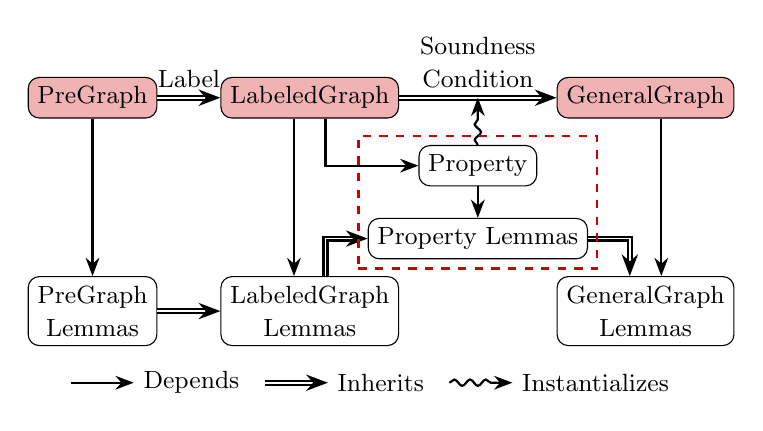
\begin{tikzpicture}
[->/.style={thick,arrows={-Stealth}},
-->/.style=	{thick,arrows={-Stealth}, decorate, decoration={snake, amplitude=.4mm,segment length=2mm,post length=2mm}},
   realG/.style={shape=rectangle, rounded corners=4pt, draw, fill=red!30},
   propG/.style={shape=rectangle, rounded corners=4pt, draw}]
\node[realG] (PG) at (0, 0) {\small PreGraph};
\node[realG] (LG) [right=0.8 of PG] {\small LabeledGraph};
\node[realG] (GG) [right=2 of LG] {\small GeneralGraph};
\draw [double, ->] (PG) -- (LG) node [pos=0.5, above] {\small Label} ;
\draw [double, ->] (LG) -- (GG) node (SC) [pos=0.5, above, align=center]
{\small Soundness \\ \small Condition};
\node[propG] (Prop) [below=0.6 of SC] {\small Property};
\node[propG] (PropL) [below=0.4 of Prop] {\small Property Lemmas};
\node[propG] (PGL) [below=2 of PG, align=center] {\small PreGraph \\\small Lemmas};
\node[propG] (LGL) [below=2 of LG, align=center] {\small LabeledGraph \\\small Lemmas};
\node[propG] (GGL) [below=2 of GG, align=center] {\small GeneralGraph \\\small Lemmas};
\draw [double, ->] (PGL) to (LGL);
\draw [->] (PG) to (PGL);
\draw [->] (Prop) to (PropL);
\draw [-->] (Prop) to (SC);
\coordinate [left=0.2 of LG.south] (LGs1);
\coordinate [left=0.2 of LGL.north] (LGLn1);
\draw [->] (LGs1) to (LGLn1);
\coordinate [right=0.2 of LG.south] (LGs2);
\coordinate [right=0.2 of LGL.north] (LGLn2);
\draw [->] (LGs2) |- (Prop);
\draw [double, ->] (LGLn2) |- (PropL);
\coordinate [right=0.2 of GG.south] (GGs);
\coordinate [left=0.2 of GGL.north] (GGLn1);
\coordinate [right=0.2 of GGL.north] (GGLn2);
\draw [double, ->] (PropL) -| (GGLn1);
\draw [->] (GGs) to (GGLn2);
\node [draw=red, thick, rectangle, dashed, fit=(Prop) (PropL)] {};
\node (legend1) [below right=0.2 and -0.3 of PGL] {\small Depends};
\coordinate[left=0.8 of legend1]  (l1);
\draw [->] (l1) to (legend1);
\node (legend2) [right=1 of legend1] {\small Inherits};
\coordinate[left=0.8 of legend2]  (l2);
\draw [double, ->] (l2) to (legend2);
\node (legend3) [right=1 of legend2] {\small Instantializes};
\coordinate[left=0.8 of legend3]  (l3);
\draw [-->] (l3) to (legend3);
\end{tikzpicture}
\end{adjustbox}
\DIFaddend \captionof{figure}{Structure of the Mathematical Graph Library}\label{fig:graphs}
\end{minipage}
  ~
  \DIFdelbegin %DIFDELCMD < \begin{minipage}[t]{0.52\textwidth}
%DIFDELCMD < %%%
\DIFdelend \DIFaddbegin \DIFadd{\hspace{0em}
  }\begin{minipage}[t]{0.5\textwidth}
  \begin{adjustbox}{scale=0.80}
\DIFaddend \centering
%DIF <  \beginpgfgraphicnamed{pregraphexp}
\DIFdelbegin %DIFDELCMD < \begin{tikzpicture}
%DIFDELCMD < [vad/.style={circle, fill=black, inner sep=0pt, minimum size=4pt},
%DIFDELCMD <  inv/.style={circle, draw=red, thick, inner sep=0pt, minimum size=4pt},
%DIFDELCMD <  ->/.style={thick, arrows={-Stealth}}]
%DIFDELCMD < \node[vad] (n1) at (0, 0) {};
%DIFDELCMD < \node at (1, 1.3) {$\m{v}_1$}; \node[inv] (n2) at (1, 1) {};
%DIFDELCMD < \node[inv] (n3) at (1, -1) {}; \node at (-2,2.25) {$\m{v}_0$}; \node[vad] (n4) at (-2,2) {}; 
%DIFDELCMD < \node[inv] (n5) at (-2,-2) {};
%DIFDELCMD < \node[vad] (n6) at (-1.7,0) {};
%DIFDELCMD < \node[inv] (n7) at (2.5,1.8) {};
%DIFDELCMD < \node[inv] (n8) at (3,-1.5) {};
%DIFDELCMD < \draw[->] (n1) to (n2);
%DIFDELCMD < \draw[->] (n1) to (n3);
%DIFDELCMD < \draw[->,dashed,red] (n3) to (n5);
%DIFDELCMD < \draw[->,dashed,red] (n2) to (n3);
%DIFDELCMD < \draw[->,dashed,red] (n2) to (n7);
%DIFDELCMD < \draw[->,dashed,red] (n2) to (n8);
%DIFDELCMD < \draw[->,dashed,red] (n3) to (n8);
%DIFDELCMD < \draw[->] (n4) to (n1);
%DIFDELCMD < \draw[->] (n1) to (n5);
%DIFDELCMD < \draw[->] (n4) to [bend left=20] (n2);
%DIFDELCMD < \draw[->] (n1) to [bend left=20] (n6);
%DIFDELCMD < \draw[->] (n6) to (n5);
%DIFDELCMD < \draw[->,dashed,red] (n8) to (n7);
%DIFDELCMD < \draw[->] (n4) to [bend right=35] (n1);
%DIFDELCMD < \node at (-0.6, 1.7) {$\m{e}$};
%DIFDELCMD < \node[vad] (n9) at (3.6, 1) {};
%DIFDELCMD < \node[inv] (n10) at (3.6, 0.5) {};
%DIFDELCMD < \draw[->] (3.4, 0) -- (4, 0);
%DIFDELCMD < \draw[->,dashed,red] (3.4, -0.5) -- (4, -0.5);
%DIFDELCMD < \node at (3.9, 1) [right=1.5pt] {\small Valid vertex};
%DIFDELCMD < \node at (3.9, 0.5) [right=1.5pt] {\small Invalid vertex};
%DIFDELCMD < \node at (3.9, 0) [right=1.5pt] {\small Valid edge};
%DIFDELCMD < \node at (3.9, -0.5) [right=1.5pt] {\small Invalid edge};
%DIFDELCMD < 

%DIFDELCMD < \end{tikzpicture}
%DIFDELCMD < %%%
%DIF <  \endpgfgraphicnamed
%DIFDELCMD < \vspace{1ex}
%DIFDELCMD < \captionof{figure}{A PreGraph with valid/invalid vertices and edges.}%%%
\DIFdelend \DIFaddbegin \DIFadd{\hspace{1.8em}
}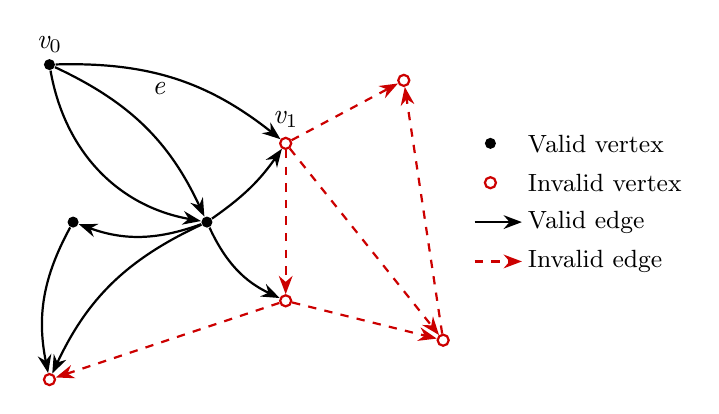
\begin{tikzpicture}
[vad/.style={circle, fill=black, inner sep=0pt, minimum size=4pt},
 inv/.style={circle, draw=red, thick, inner sep=0pt, minimum size=4pt},
 ->/.style={thick, arrows={-Stealth}}]
\node[vad] (n1) at (0, 0) {};
\node at (1, 1.3) {$\m{v}_1$}; \node[inv] (n2) at (1, 1) {};
\node[inv] (n3) at (1, -1) {}; \node at (-2,2.25) {$\m{v}_0$}; \node[vad] (n4) at (-2,2) {}; 
\node[inv] (n5) at (-2,-2) {};
\node[vad] (n6) at (-1.7,0) {};
\node[inv] (n7) at (2.5,1.8) {};
\node[inv] (n8) at (3,-1.5) {};
\draw[->] (n1) to [bend right=10] (n2);
\draw[->] (n1) to [bend right=20] (n3);
\draw[->,dashed,red] (n3) to (n5);
\draw[->,dashed,red] (n3) to (n8);
\draw[->,dashed,red] (n2) to (n3);
\draw[->,dashed,red] (n2) to (n7);
\draw[->,dashed,red] (n2) to (n8);
\draw[->,dashed,red] (n8) to (n7);
\draw[->] (n4) to [bend left=20] (n1);
\draw[->] (n1) to [bend right=20] (n5);
\draw[->] (n4) to [bend left=20] (n2);
\draw[->] (n1) to [bend left=20] (n6);
\draw[->] (n6) to [bend right=20] (n5);
\draw[->] (n4) to [bend right=35] (n1);
\node at (-0.6, 1.7) {$\m{e}$};
\node[vad] (n9) at (3.6, 1) {};
\node[inv] (n10) at (3.6, 0.5) {};
\draw[->] (3.4, 0) -- (4, 0);
\draw[->,dashed,red] (3.4, -0.5) -- (4, -0.5);
\node at (3.9, 1) [right=1.5pt] {\small Valid vertex};
\node at (3.9, 0.5) [right=1.5pt] {\small Invalid vertex};
\node at (3.9, 0) [right=1.5pt] {\small Valid edge};
\node at (3.9, -0.5) [right=1.5pt] {\small Invalid edge};

\end{tikzpicture}
\end{adjustbox}

\captionof{figure}{PreGraph with valid/invalid vertices/edges.}\DIFaddend \label{fig:pregraph}
\end{minipage}
\DIFdelbegin %DIFDELCMD < \end{adjustbox}
%DIFDELCMD <  \begin{figure}
%DIFDELCMD < 	%%%
\begin{eqnarray*}
     	\DIFdelFL{\begin{aligned}
    	\mathrm{path} \; \defeq \; &(\m{v}_0, [e_0, e_1, \dots, e_k]) \\ 
    	\mathtt{s\_evalid}(\gamma, e) \; \defeq \; & \mathtt{E}_{\gamma}(e) /| 
    	\mathtt{V}_{\gamma}(\mathtt{src}_{\gamma}(e)) /| 
    	\mathtt{V}_{\gamma}(\mathtt{dst}_{\gamma}(e)) \\
		\mathtt{valid\_path}\big(\gamma, (\m{v},[])\big) \;\defeq \; & \mathtt{V}_{\gamma}(\m{v})\\
		\mathtt{valid\_path}\big(\gamma, (\m{v},[e_1,e_2,\dots,e_n])\big) \; \defeq \; &\m{v}=\mathtt{src}_{\gamma}(e_1) \wedge \mathtt{s\_evalid}(\gamma,e_1) \wedge \null \\
    &\mathtt{dst}_{\gamma}(e_1)=\mathtt{src}_{\gamma}(e_2) \wedge \null\\
    &\mathtt{s\_evalid}(\gamma, e_2) \wedge \dots /| \mathtt{dst}_{\gamma}(e_{n-1})=\mathtt{src}_{\gamma}(e_n) \\ 
        \mathtt{end}\big(\gamma, (\m{v}, [])\big)\;\defeq\;& \m{v}\\
      	\mathtt{end}\big(\gamma, (\m{v},[e_1,e_2,\dots,e_n])\big)\;\defeq\;&
      	\mathtt{dst}_{\gamma}(e_{n})\\
      	\gamma \vDash s \overset{\m{p}}{\leadsto} t \;\defeq\; &
        \mathtt{valid\_path}(\gamma, p)\wedge
        \mathtt{fst}(p)=s \wedge \mathtt{end}(\gamma,p)=t \\
        \gamma_1 \cong \gamma_2 \; \defeq \; & 
        	\forall e.~\mathtt{E}_{\gamma_1}(e) <=> \mathtt{E}_{\gamma_2}(e) /| \forall \m{v}.~\mathtt{V}_{\gamma_1}(\m{v}) <=> \mathtt{V}_{\gamma_1}(\m{v}) /| \null \\
        	&\forall e.~\mathtt{E}_{\gamma_1}(e) ==> \mathtt{src}_{\gamma_1}(e) = \mathtt{src}_{\gamma_2}(e) /| \mathtt{dst}_{\gamma_1}(e) = \mathtt{dst}_{\gamma_2}(e) \\
       	\gamma \smallsetminus S \; \defeq \; 
       	 	&{\mathcal{V}}_{\gamma'} = {\mathcal{V}}_{\gamma} /| 
          {\mathcal{E}}_{\gamma'} = {\mathcal{E}}_{\gamma} /| \null \\
          &{\mathtt{src}}_{\gamma'} = {\mathtt{src}}_{\gamma} /|
          {\mathtt{dst}}_{\gamma'} = {\mathtt{dst}}_{\gamma} /| \null \\
       	 	&\gamma'_{\mathtt{V}} = \Big(\lambda x.~ \gamma_{\mathtt{V}}(x) /| \lnot S_{\mathtt{V}}(x)\Big) /| \null \\ 
       	 	&\gamma'_{\mathtt{E}} = \Big(\lambda x.~ \gamma_{\mathtt{E}}(x) /| \lnot S_{\mathtt{E}}(x)\Big)\\
\mathrm{MathGraph}(\gamma)\,\defeq\,\Big\{
          \mathtt{null}:\; & V\\ 
          \mathtt{valid\_graph}:\;& \forall e\,.\,\mathtt{evalid}(\gamma, e) \Rightarrow
          \mathtt{vvalid}\big(\gamma, \mathtt{src}(\gamma, e)\big)\wedge \null \\
          & \qquad \big(\m{e} = \mathtt{null} \vee \mathtt{vvalid}(\gamma, \m{e})\big)\\
          \mathtt{valid\_not\_null}:\;& \forall \m{v}\,.\,\mathtt{vvalid}(\gamma, \m{v})
          \Rightarrow \m{v} \neq \mathtt{null} \Big\} \\
        \mathrm{LstGraph}(\gamma)\,\defeq\, \Big\{
          \mathtt{out}:\; & V \rightarrow E\\
          \mathtt{only\_one\_edge}:\; & \forall \m{v},\,e\,.\,
          \mathtt{vvalid}(\gamma, \m{v}) \Rightarrow \\
          & \Big(\mathtt{src}(\gamma, e) =\m{v} \wedge
          \mathtt{evalid}(\gamma, e)\Big) \Leftrightarrow
          e = \mathtt{out}(\m{v})\\
         \mathtt{acyclic\_path}:\; & \forall \m{v},\,p\,.\,
         \gamma \vDash \m{v} \overset{p}{\leadsto} \m{v} \Rightarrow p = (\m{v},[])\Big\} \\
       	\mathrm{FiniteGraph}(\gamma)\,\defeq\, \Big\{
          \mathtt{finite\_\m{v}}:\;&\exists\, S_\m{v},\, M_\m{v}\;\text{s.t.}\;\lvert S_\m{v}\rvert
          \leq M_\m{v} \wedge
          \forall \m{v}\,.\, \mathtt{vvalid}(\gamma,\m{v})\Rightarrow \m{v}\,\in\,S_\m{v}\\
          \mathtt{finite\_e}:\;&\exists\, S_e,\, M_e\;\text{s.t.}\;\lvert S_e\rvert
          \leq M_e \wedge
          \forall e\,.\, \mathtt{evalid}(\gamma,e)\Rightarrow e\,\in\,S_e \Big\}
    	\end{aligned}
    }\end{eqnarray*}
%DIFAUXCMD
%DIFDELCMD < \caption{%
{%DIFAUXCMD
\DIFdelFL{Some Graph definitions}}
%DIFAUXCMD
%DIFDELCMD < \label{fig:graphdefns}
%DIFDELCMD < \vspace{-1em}
%DIFDELCMD < \end{figure} 
%DIFDELCMD < %%%
\DIFdelend \DIFaddbegin \vspace{1.5ex}

 
\subsection{\texorpdfstring{\DIFadd{Definitions of Graphs}}{XXX}}\label{sec:mathinfra}

\DIFaddend Our first challenge is that graph theory is usually based on
\emph{set theory} but our formalization in Coq is
based on \emph{type theory}. 
\DIFdelbegin \DIFdel{We choose to formalize graph theory
directly in Coq instead }\DIFdelend \DIFaddbegin \DIFadd{Instead }\DIFaddend of formalizing set theory \DIFaddbegin \DIFadd{in Coq }\DIFaddend and then building
graph theory atop it\DIFdelbegin \DIFdel{to }\DIFdelend \DIFaddbegin \DIFadd{, we formalize graph theory
directly in Coq, as this lets us }\DIFaddend take advantage of Coq's built-in
support for type-related constructions.
To \DIFdelbegin \DIFdel{balance }\DIFdelend \DIFaddbegin \DIFadd{reconcile }\DIFaddend the dichotomy between
\DIFdelbegin \DIFdel{the generality and the speciality of the library , we divide the
concept of graph into three structures,
}\DIFdelend \DIFaddbegin \DIFadd{a very general library and highly specialized examples, we develop
our graphs gradually over three linked concepts:
}\DIFaddend PreGraph, LabeledGraph and GeneralGraph\DIFdelbegin \DIFdel{, arranged in a hierarchy}\DIFdelend .
Figure~\ref{fig:graphs} shows the
architecture of the library.

\hide{The most basic kind of graph is PreGraph, out of which we build
LabeledGraph, and which in turn are used
to build GeneralGraphs. Each kind has some lemmas and also inherits the lemmas of the
previous kind.  The dashed box represents a ``plugin'' system for attaching arbitrary
properties to LabeledGraphs (\ref{subsec:graphplugins}). } 

\paragraph{PreGraph.}
A PreGraph is a hextuple $(\mathcal{V}, \mathcal{E}, \mathtt{V}, \mathtt{E}, \mathtt{src}, \mathtt{dst})$.  \DIFaddbegin \DIFadd{Arguments }\DIFaddend $\mathcal{V}$ and $\mathcal{E}$ are the underlying
carrier types of vertices and edges.  $\mathtt{V}$ and $\mathtt{E}$ are predicates over
$\mathcal{V}$ and $\mathcal{E}$ that specify the notion
of \emph{validity} in the graph.  Finally, $\mathtt{src}$ and $\mathtt{dst}: \DIFaddbegin \DIFadd{\mathcal{E} -> \mathcal{V}}\DIFaddend$ map each edge to
its source and destination.


The benefits of introducing validity are twofold. The first is a
neat resolution of the incompatibility between type theory and set theory.
In set theory, one
element can belong to multiple sets, and
adding or removing vertices or edges is as easy as altering
the set directly to represent the result of the operation.
In type theory, however, a term can only belong
to one type, which makes it difficult\hide{if not impossible}
to analogously change the
type to represent the result. As is common practice, the
predicates $\mathtt{V}$ and $\mathtt{E}$ specify whether a vertex/edge is \emph{valid}
(in the graph) or \emph{invalid} (out). Adding or removing vertices/edges
is as simple as weakening or strengthening these two predicates.

The second benefit is the ability to represent incomplete graphs.
Consider starting from a graph\DIFaddbegin \DIFadd{~}\DIFaddend $\gamma$ and then removing a subgraph; the remaining
``doughnut'' structure is \textbf{not} necessarily a graph, since there may be dangling
edges pointing into the ``hole''.  Figure \ref{fig:pregraph} shows just such a situation,
where a connected graph (everything \DIFaddbegin \DIFadd{that }\DIFaddend is reachable from $\m{v}_0$) has had the connected
subgraph reachable from $\m{v}_1$ removed\DIFdelbegin \DIFdel{; }\emph{\DIFdel{e.g.}}%DIFAUXCMD
\DIFdel{, }\DIFdelend \DIFaddbegin \DIFadd{, thus leaving }\DIFaddend the edge $e$ \DIFdelbegin \DIFdel{is }\DIFdelend dangling.
The last conjunct in the $\m{findS}$ relation from Figure~\ref{fig:find} is an example
of where a real verification needs to reason about just such a doughnut, in particular
to specify that the unreachable portion of a graph has not changed.


\hide{an incomplete graph,
where vertices $v_0$ and $v_1$
are the source and destination of a valid edge $e_0$. Both
vertices are in $\mathcal{V}$, but $v_0$ is valid
and $v_1$ is not, meaning $v_1$ is not in the
graph. Drawing $v_1$ in Figure \ref{fig:pregraph} only indicates
that $d(e_0) = v_1$.
Incomplete graphs of this sort are needed, \emph{e.g.}, by programs
that traverse selective portions of graphs and manipulate them under
certain criteria.
After the traversal, the graph $g$ can be partitioned into two parts: the subgraph
$g_1$, which is composed of vertices and edges processed by the algorithm,
and the residue $g_2$, which is the difference $g - g_1$. In
the specification of the program, it may be necessary to state that
$g_2$ is unchanged. However, $g_2$ is not guaranteed to be a ``well-formed''
graph in the conventional sense:
if $g$ is an undirected graph,
$g_2$ is just a collection of \note[disconnected?]{connected} components,
and if $g$ is a directed graph, then $g_2$ may contain dangling edges or
vertices. PreGraph is accommodating enough to permit reasoning
about~$g_2$ in either case.}

\DIFaddbegin \begin{figure}
  \begin{minipage}{.52\textwidth}
  \begin{equation*}
  {\DIFaddFL{\footnotesize
  \begin{array}{r@{}c@{}l}
    	\mathrm{path} \; &\defeq \;& (\m{v}_0, [e_0, e_1, \dots, e_k]) \\
      \mathtt{end}\big(\gamma, (\m{v}, [])\big)\;&\defeq\;& \m{v}\\
      \mathtt{end}\big(\gamma, (\m{v},[e_1,\dots,e_n])\big)\;&\defeq\;&
      \mathtt{dst}_{\gamma}(e_{n}) \\
      \mathtt{s\_evalid}(\gamma, e) \; &\defeq \;& \mathtt{E}_{\gamma}(e) /| \null \\
      &&\mathtt{V}_{\gamma}(\mathtt{src}_{\gamma}(e)) /| \null \\
      &&\mathtt{V}_{\gamma}(\mathtt{dst}_{\gamma}(e)) \\
      \mathtt{valid\_path}\big(\gamma, (\m{v},[])\big) \;&\defeq \;& \mathtt{V}_{\gamma}(\m{v})\\
      \mathtt{valid\_path}\big(\gamma, (\m{v},[e_1,e_2,\dots,e_n])\big) \; &\defeq \;& \m{v}=\mathtt{src}_{\gamma}(e_1) \wedge \null \\
      &&\mathtt{s\_evalid}(\gamma,e_1) \wedge \null \\
      &&\mathtt{dst}_{\gamma}(e_1)=\mathtt{src}_{\gamma}(e_2) \wedge \null \\
      &&\mathtt{s\_evalid}(\gamma, e_2) \wedge \dots /| \null \\
      &&\mathtt{dst}_{\gamma}(e_{n-1})=\mathtt{src}_{\gamma}(e_n)
  \end{array}}}
  \end{equation*}
  \end{minipage}\begin{minipage}{.5\textwidth}
  \begin{equation*}
  {\DIFaddFL{\footnotesize
  \begin{array}{r@{}c@{}l}
      \gamma_1 \cong \gamma_2 \; &\defeq\;&
        \forall e.~\mathtt{E}_{\gamma_1}(e) <=> \mathtt{E}_{\gamma_2}(e) /| \null \\
        &&\forall \m{v}.~\mathtt{V}_{\gamma_1}(\m{v}) <=> \mathtt{V}_{\gamma_1}(\m{v}) /| \null \\
        &&\forall e.~\mathtt{E}_{\gamma_1}(e) ==> \mathtt{src}_{\gamma_1}(e) = \mathtt{src}_{\gamma_2}(e) /| \null \\
        &&\hspace{5.9em} \mathtt{dst}_{\gamma_1}(e) = \mathtt{dst}_{\gamma_2}(e) \\
      \gamma |= s \overset{\m{p}}{\leadsto} t \;&\defeq\;&
        \mathtt{valid\_path}(\gamma, p)\wedge \null \\
        &&\mathtt{fst}(p)=s \wedge \mathtt{end}(\gamma,p)=t \\
      \gamma \smallsetminus S \; &\defeq \;&
          \Big(\mathcal{V}_{\gamma},\mathcal{E}_{\gamma}, \mathtt{src}_{\gamma}, \mathtt{dst}_{\gamma}, \\
          &&\qquad \lambda x.~ \gamma_{\mathtt{V}}(x) /| \lnot S_{\mathtt{V}}(x), \\
          &&\qquad \lambda x.~ \gamma_{\mathtt{E}}(x) /| \lnot S_{\mathtt{E}}(x)\;\Big)\\
          && \hspace{-1cm}\mathit{reachable}(\gamma, x)\;\defeq\;\big\{t \mid \exists\,p\,.\, \gamma |= x \overset{\m{p}}{\leadsto} t\big\}
  \end{array}}}
  \end{equation*}
  \end{minipage}
\vspace{-.7em}
\caption{\DIFaddFL{Some PreGraph definitions}}
\label{fig:pregraphdefs}
\vspace{-1em}
\end{figure}

%DIF > 

\DIFaddend We define many fundamental graph concepts on PreGraphs,
including structures like \emph{path}$^{*}$, predicates
such as \emph{is\_cyclic} and \emph{reachable}$^{*}$,
operations such as \emph{add\_vertex}
and \emph{remove\_edge}, and relations between PreGraphs such
as \emph{structurally\_identical}$^{*}$ and \emph{subgraph}.
Definitions of the concepts marked with asterisks are
shown in Figure \DIFdelbegin \DIFdel{\ref{fig:graphdefns} }\DIFdelend \DIFaddbegin \DIFadd{\ref{fig:pregraphdefs} }\DIFaddend to give a flavor
of the subtleties involved in getting definitions that
really work.
These general concepts, together with around 500 derived lemmas,
provide a
solid foundation for more specific theorems needed in concrete
verifications.

\hide{
In {\color{magenta}Figure \ref{fig:pregraph}}, valid vertices satisfy
$V$ and invalid vertices are just of type $VT$ but do not satisfy
$V$. Importantly, both kinds of vertices are legally part of the
PreGraph. Finally, $s$ and $d$ are functions that map an edge to its
source and destination respectively; {\color{orange}this means that
PreGraphs model directed graphs.}  With an eye to flexibility, we make
no further requirements of a legal PreGraph, not even a specific
notion of how the four sets are related.  Indeed, the PreGraph in
Figure \ref{fig:pregraph} contains invalid vertices and edges in an
arbitrary configuration.

Many graph concepts such as \emph{path}, \emph{reachability}, and \emph{subgraph} are
defined on PreGraphs. In \S\ref{fig:find} we saw \emph{reachable}, written
{\color{orange}
$\m{a} \mathrel{{\stackrel{\gamma~}{\leadsto^{1}}}} \m{b}$. It means that a and b are in $V(\gamma)$ and that there exists an edge (in $E(\gamma)$)
that goes from a to b.}
The reflexive, transitive closure on \emph{reachable} is written
$\m{a} \accentset{\gamma}{\leadsto}^{\star} \m{b}$, and
$\neg (\m{a} \accentset{\gamma}{\leadsto}^{\star} \m{b})$
is written
$\m{a} \accentset{\gamma}{\not\leadsto}^{\star} \m{b}$
$\m{a} \mathrel{{\stackrel{\gamma~}{\not\leadsto^{\star}}}} \m{b}$.

PreGraph's ability to reason about missing vertices and edges is convenient when
verifying real programs. Suppose some $\gamma$ satisfied some stronger notion of
``well-formed'', in the sense that valid vertices have only valid edges and
vice versa. Could we then subtract some vertices and edges from it and reason about the
resulting structure? This is precisely what we needed to do in \ref{fig:find}, where
we argued for a condition of congruence on
$\gamma \smallsetminus (v \in \gamma \mid \m{x}
\mathrel{{\stackrel{\gamma~}{\leadsto^{\star}}}} \m{v})$.
A strong notion of well-formedness may have stopped us short at this point,
declaring the structure ill-formed because of the dangling edges
pointing to recently-removed vertices.
A PreGraph is more accommodating, since
it produces a fresh PreGraph after this selective subtraction
and then allows us to go ahead and reason about congruence as we need to.
}

\hide{
For example, consider the difference of two graphs, $\gamma_1
- \gamma_2$.  Even if both of these graphs are ``well-formed'' to begin with, in the
sense that valid vertices have only valid edges and vice versa, their difference
may not be since there may be dangling edges pointing to the
now-removed vertices of $\gamma_2$.} 

\hide
{In \S\ref{sec:spacegraph} we will tie a mathematical graph $\gamma$ to
a spatial graph predicate
$\p{graph}(x, \gamma)$.   As we will see, a $\p{graph}$ ``owns'' only the
spatial portion of $\gamma$ that is reachable
from $x$ even though $\gamma$ may have other valid vertices.
} 




\vspace{-0.75ex}

\paragraph{LabeledGraph.}
A LabeledGraph is septuple $(\mathrm{PreGraph},\ma{L_{V}},\ma{L_{E}},\ma{L_{G}}, \mathtt{vl},\mathtt{el},\mathtt{gl})$ that augments a PreGraph with \emph{labels} on
vertices, edges, and/or the graph as a whole. $\ma{L_{V}}$, $\ma{L_{E}}$, and $\ma{L_{G}}$
are the associated carrier types\DIFdelbegin \DIFdel{; }\DIFdelend \DIFaddbegin \DIFadd{, and }\DIFaddend $\mathtt{vl}$, $\mathtt{el}$, and $\mathtt{gl}$
are the labeling functions themselves.
\DIFdelbegin \DIFdel{The need for such labels is that many }\DIFdelend \DIFaddbegin \DIFadd{Many }\DIFaddend classic graph problems\DIFaddbegin \DIFadd{, }\DIFaddend from union-find (node ranks)
to Dijkstra (edge weights)\DIFdelbegin \DIFdel{require them}\DIFdelend \DIFaddbegin \DIFadd{, require such labels}\DIFaddend .
The need for a label on the graph as a whole
is \DIFdelbegin \DIFdel{a little more subtle}\DIFdelend \DIFaddbegin \DIFadd{not as obvious}\DIFaddend ; in \S\ref{sec:certigc} we use one in the garbage collector
to keep track of \DIFdelbegin \emph{\DIFdel{e.g.}} %DIFAUXCMD
\DIFdelend the number of generations and their boundaries.
Since \DIFaddbegin \DIFadd{every }\DIFaddend LabeledGraph is built on \DIFaddbegin \DIFadd{a }\DIFaddend PreGraph, it inherits all \DIFdelbegin \DIFdel{PreGraph }\DIFdelend \DIFaddbegin \DIFadd{of the 
PreGraph's }\DIFaddend lemmas via
Coq's \emph{type coercion} mechanism \DIFdelbegin \DIFdel{, while enabling }\DIFdelend \DIFaddbegin \DIFadd{while also opening the doors to 
}\DIFaddend additional lemmas involving \DIFaddbegin \DIFadd{its own }\DIFaddend labels.



\DIFdelbegin %DIFDELCMD < \hide{\paragraph{LabeledGraph.}
%DIFDELCMD < A LabeledGraph is a PreGraph with the addition of \emph{labels} on
%DIFDELCMD < vertices, edges, and/or the graph as a whole. The need for such labels
%DIFDELCMD < is fairly clear; the bare structure of a graph can only
%DIFDELCMD < contain so much information, and many classic graph problems
%DIFDELCMD < such as graph coloring, shortest path, and network flow rely on
%DIFDELCMD < additional information in the form of labels. In our architecture, a
%DIFDELCMD < LabeledGraph inherits any lemmas proved about its associated PreGraph.
%DIFDELCMD < In addition, we can define additional lemmas that use labels,
%DIFDELCMD < \emph{e.g.} the union-find graph has an integer label denoting \emph{rank}.
%DIFDELCMD < We could prove a lemma that running \texttt{find} does not alter
%DIFDELCMD < any vertex's rank.
%DIFDELCMD < \hide{add string labels to edges and reason about a trie.}}
%DIFDELCMD < %%%
\DIFdelend \DIFaddbegin \hide{\paragraph{LabeledGraph.}
A LabeledGraph is a PreGraph with the addition of \emph{labels} on
vertices, edges, and/or the graph as a whole. The need for such labels
is fairly clear; the bare structure of a graph can only
contain so much information, and many classic graph problems
such as graph coloring, shortest path, and network flow rely on
additional information in the form of labels. In our architecture, a
LabeledGraph inherits any lemmas proved about its associated PreGraph.
In addition, we can define additional lemmas that use labels,
\emph{e.g.} the union-find graph has an integer label denoting \emph{rank}.
We could prove a lemma that running \li{find} does not alter
any vertex's rank.
\hide{add string labels to edges and reason about a trie.}}
\DIFaddend 




\vspace{-0.75ex}
\paragraph{GeneralGraph.}
PreGraphs and LabeledGraphs let us state
and prove many useful lemmas that follow essentially by the nature
of our graph constructions. However, when proving the correctness of graph
algorithms, we often need more specificity in our mathematical graphs
so that we may model the real program's behaviors closely.
For example, the \p{uf\_graph} used in \DIFdelbegin \texttt{\DIFdel{find}}
%DIFAUXCMD
\DIFdel{restricted }\DIFdelend \DIFaddbegin \li{find}
\DIFadd{restricts }\DIFaddend each vertex to having exactly one out-edge.
On the other hand, these restrictions vary greatly by algorithm, so we do not
want to bake them into our core definitions.
We achieve this flexibility using GeneralGraphs, which augment
LabeledGraphs by adding arbitrarily complex ``soundness conditions'', indicated in
Figure~\ref{fig:graphs} with a dashed border.
Further, the type coercion we described earlier continues to apply,
meaning that a GeneralGraph can seamlessly behave like \DIFdelbegin \DIFdel{a
}\DIFdelend \DIFaddbegin \DIFadd{its internal
}\DIFaddend LabeledGraph or a PreGraph, thereby inheriting their lemmas.
This combination of specificity and generality
\DIFdelbegin \DIFdel{is
what }\DIFdelend makes GeneralGraphs versatile. Moreover, we can
compose complicated soundness conditions from reusable pieces,
further enabling code sharing between algorithms.







\subsection{\texorpdfstring{Composing \DIFdelbegin \DIFdel{soundness plugins}\DIFdelend \DIFaddbegin \DIFadd{Soundness Plugins}\DIFaddend}{XXX}}
\label{subsec:graphplugins}
\DIFaddbegin \begin{figure}
{\footnotesize
\begin{align*}
  \DIFaddFL{\mathrm{MathGraph}(\gamma)\,}& \DIFaddFL{\defeq \,\left\{
  \begin{aligned}
    \mathtt{null}:&\; V\\
    \mathtt{valid\_graph}:&\;
    \forall e\,.\,\mathtt{evalid}(\gamma, e) \Rightarrow
      \mathtt{vvalid}\big(\gamma, \mathtt{src}(\gamma, e)\big)\wedge
      \big(\m{e} = \mathtt{null} \vee \mathtt{vvalid}(\gamma, \m{e})\big)\\
    \mathtt{valid\_not\_null}:&\; \forall \m{v}\,.\,\mathtt{vvalid}(\gamma, \m{v})
    \Rightarrow \m{v} \neq \mathtt{null}
  \end{aligned} \right\}}\\
  \DIFaddFL{\mathrm{LstGraph}(\gamma)\,}&\DIFaddFL{\defeq\, \left\{
  \begin{aligned}
    \mathtt{out}:&\; V \rightarrow E\\
    \mathtt{only\_one\_edge}:&\;
    \forall \m{v},\,e\,.\,\mathtt{vvalid}(\gamma, \m{v}) \Rightarrow
    \big(\mathtt{src}(\gamma, e) =\m{v} \wedge
    \mathtt{evalid}(\gamma, e)\big) \Leftrightarrow e = \mathtt{out}(\m{v})\\    
  \mathtt{acyclic\_path}:&\; \forall \m{v},\,p\,.\,
  \gamma |= \m{v} \overset{p}{\leadsto} \m{v} \Rightarrow p = (\m{v},[]) \\
  \end{aligned} \right\}}\\
  \DIFaddFL{\mathrm{FiniteGraph}(\gamma)\,}&\DIFaddFL{\defeq\, \left\{
  \begin{aligned}
      \mathtt{finite\_v}:&\;\exists\, S_\m{v},\, n.~\;\lvert S_\m{v}\rvert
      \leq n \wedge
      \forall \m{v}\,.\, \mathtt{vvalid}(\gamma,\m{v})\Rightarrow \m{v}\,\in\,S_\m{v}\\
      \mathtt{finite\_e}:&\;\exists\, S_e,\, n.~\;\lvert S_e\rvert
      \leq n \wedge
      \forall e\,.\, \mathtt{evalid}(\gamma,e)\Rightarrow e\,\in\,S_e\\
  \end{aligned}  \right\}}\\
\end{align*}}
\vspace*{-3em}
\caption{\DIFaddFL{Some GeneralGraph definitions}}
\label{fig:gengraphdefs}
\vspace{-1.5em}
\DIFaddendFL 

\DIFaddbeginFL \end{figure} 

\DIFaddend \hide{Our entire library of formal
graph theory is developed around the
three graph structures above. The theorems about the first two
are universal, while some theorems about GeneralGraph
are developed on demand because soundness conditions vary by
algorithm.}
Soundness conditions are often specific to each algorithm, but they feature some recurring themes.
We take advantage of this pattern by developing \emph{soundness plugins}, \emph{i.e.} definitions of soundness
conditions along with related lemmas.  By combining these plugins
we can describe the soundness condition we need for a particular
algorithm.  When proving lemmas about the resulting combination,
we can use known facts about the separate plugins, in addition to
lemmas that emerge due to the various combinations.  This complexity
is managed smoothly by Coq's typeclass system, increasing the
compositionality of the system.
Consider the following oft-used graph properties:

\begin{itemize}
\vspace{-1ex}
\item \DIFaddbegin \p{BiGraph}\DIFadd{: there are exactly two outgoing edges per vertex
}\item \DIFadd{$\p{LstGraph}^{*}$: the graph is structured like a list, meaning that every 
vertex has one outgoing edge, and there no loops except trivial self-loops 
of length $0$, signifying the end of the ``list"
}\item \DIFaddend $\p{MathGraph}^{*}$: \DIFdelbegin \DIFdel{all valid edges must have }\DIFdelend \DIFaddbegin \DIFadd{every valid edge has }\DIFaddend a valid source vertex\DIFdelbegin \DIFdel{; the destination vertex must either be valid or be }\DIFdelend \DIFaddbegin \DIFadd{,
and its destination vertex is either valid or is }\DIFaddend a 
special invalid \DIFdelbegin \DIFdel{node }\DIFdelend \DIFaddbegin \DIFadd{vertex }\DIFaddend called \p{null}
\item $\p{FiniteGraph}^{*}$: the sets of valid vertices and edges are both finite
\hide{More subtly, consider that many real data structures use special null values to
represent unused nodes.  The  property introduces this concept---
\emph{i.e.} some special invalid nodes are allowed to appear as
destinations for valid edges.} 
\DIFdelbegin %DIFDELCMD < \item %%%
\item%DIFAUXCMD
\DIFdel{$\p{LstGraph}^{*}$: the graph is list-like: each vertex has only one outgoing edge; no nontrivial loops
}%DIFDELCMD < \item \p{BiGraph}%%%
\item%DIFAUXCMD
\DIFdel{: there are exactly two outgoing edges per node
}\DIFdelend \DIFaddbegin 



\DIFaddend \end{itemize}
Definitions of the concepts marked with asterisks are
shown in Figure~\DIFdelbegin \DIFdel{\ref{fig:graphdefns} }\DIFdelend \DIFaddbegin \DIFadd{\ref{fig:gengraphdefs} }\DIFaddend for illustration.
\DIFdelbegin %DIFDELCMD < 

%DIFDELCMD < %%%
\DIFdelend \hide{As a first step, we can prove many general, reusable lemmas
about these properties. However, these properties are still
too general to model a real program. The next step is to compose
these plugins to arrive at a more specific set of restrictions
that more closely models our particular graph.}
We can compose
\p{LstGraph}, \p{MathGraph}, and \p{FiniteGraph}
together into a new plugin called \p{LiMaFin}, which, incidentally, is
the soundness condition of mathematical \p{uf\_graph}
we used to verify \DIFdelbegin \texttt{\DIFdel{find}} %DIFAUXCMD
\DIFdelend \DIFaddbegin \li{find} \DIFaddend in
Figure~\ref{fig:find}.  In our verification of \DIFdelbegin \texttt{\DIFdel{mark}} %DIFAUXCMD
\DIFdelend \DIFaddbegin \li{mark} \DIFaddend in
Figure~\ref{fig:markgraph}, we use a similar soundness condition
\p{BiMaFin}, which uses \p{BiGraph} instead of \p{LstGraph}.
The commonalities and differences between \p{LiMaFin}
and \p{BiMaFin} are readily apparent from their construction\DIFaddbegin \DIFadd{, 
and can be exploited for proof reuse}\DIFaddend .


\iffalse
\marginpar{\tiny \color{blue} Maybe move this somewhere.}
{\color{magenta}Coq also handles our notion of inherited
lemmas seamlessly: in our verfication of Find, we
work directly with a \p{LiMaFin} GeneralGraph, but, as
we saw, we still use properties such as reachability
and operations such as selective subtraction, which are defined on the
embedded PreGraph, not the GeneralGraph.
Coq handles the appropriate coercions with
remarkable elegance.}
\fi

\iffalse
\subsection{Reasoning about relations between graphs} 

\marginpar{\color{blue} \tiny Needs revised examples based on new Orientation.}

{\color{magenta} In Figure~\ref{fig:markgraph} we defined the relation
$\m{mark}(\gamma, \tx x, \gamma')$
for the graph marking algorithm.  Similarly, we define $\m{span}$ for the
spanning tree program
and $\m{copy}$ for the graph copy program.
These relations all capture how the graph has changed from before to after the program
execution.  By specifying $\m{copy}$ relationally
rather than functionally we avoid explicitly modeling how the memory
allocator works, a major advantage.

As previously mentioned, we reuse $\m{mark}$ and its
related lemmas to prove facts about spanning tree and graph copy
because the latter two programs mark nodes as they work.
Accordingly, we can reuse facts such as the following:
\[
\begin{array}{@{}l@{}}
\text{if } \gamma(x)=(0, v_1, \dots,v_n), \m{mark1}(\gamma, x, \gamma_1),
\text{ and } \forall i, \m{mark}(\gamma_i,v_i,\gamma_{i+1}) \text{ then } \m{mark}(\gamma,x,\gamma_{n+1}).
\end{array}
\]
}
\fi

\section{Defining and reasoning about spatial graphs}
\label{sec:spacegraph}
\DIFdelbegin %DIFDELCMD < \begin{figure}
%DIFDELCMD < %%%
\[
\DIFdelFL{\begin{array}{lcl}
\sigma |= P * Q & \defeq & \exists \sigma_1, \sigma_2.~ (\sigma_1 \oplus \sigma_2 = \sigma) /| (\sigma_1 |= P) /| (\sigma_2 |= 2)\\
\sigma |= P --* Q & \defeq & \forall \sigma_1, \sigma_2.~ (\sigma_1 \oplus \sigma = \sigma_2) /| (\sigma_1 |= P) => (\sigma_2 |= Q) \\
\sigma |= P --o Q & \defeq & \exists \sigma_1, \sigma_2.~ (\sigma_1 \oplus \sigma = \sigma_2) /| (\sigma_1 |= P) /| (\sigma_2 |= Q) \\
\sigma |= P ** Q & \defeq & \exists \sigma_1, \sigma_2, \sigma_3.~ (\sigma_1 \oplus \sigma_2 \oplus \sigma_3 = \sigma) /| (\sigma_1 \oplus \sigma_2 |= P) /| (\sigma_2 \oplus \sigma_3 |= Q)
\end{array}
}\]
%DIFAUXCMD
%DIFDELCMD < \caption{%
{%DIFAUXCMD
\DIFdelFL{Separation logic connectives; $\oplus$ is the join operation on states, }\emph{\DIFdelFL{e.g.}} %DIFAUXCMD
\DIFdelFL{a disjoint union on heaps}}
%DIFAUXCMD
%DIFDELCMD < \label{fig:seplogsem}
%DIFDELCMD < \vspace*{-1em}
%DIFDELCMD < \end{figure}  
%DIFDELCMD < %%%
\DIFdelend \DIFaddbegin 


\DIFaddend To prove the functional correctness of graph-manipulating algorithms implemented in a real language, we need to 
\DIFaddbegin \DIFadd{(1) }\DIFaddend connect the heap representation of graphs \DIFdelbegin \DIFdel{, }\DIFdelend \DIFaddbegin \DIFadd{to }\DIFaddend the memory model of the 
programming language, and \DIFdelbegin \DIFdel{the }\DIFdelend \DIFaddbegin \DIFadd{(2) connect the memory model to the }\DIFaddend mathematical 
properties of \DIFaddbegin \DIFadd{abstract }\DIFaddend graphs from \S\ref{sec:mathgraph}.
The first of these \DIFaddbegin \DIFadd{challenges }\DIFaddend turns out to be surprisingly subtle\DIFdelbegin \DIFdel{as we shall see in \S\ref{sec:fixpointfail} and \S\ref{sec:goodgraph}}\DIFdelend \DIFaddbegin \DIFadd{: 
the standard tactic of leveraging the \infrulestyle{Frame} rule 
works well for tree-manipulating programs, but fails for graph-manipulating programs.
We review the standard treatment for trees~(\S\ref{sec:seplogtrees}), 
point out the issue with graphs~(\S\ref{sec:fixpointfail}),
and propose a fix for this~(\S\ref{sec:goodgraph})}\DIFaddend .  
The main challenge \DIFdelbegin \DIFdel{for the others }\DIFdelend \DIFaddbegin \DIFadd{thereafter }\DIFaddend is to engineer a framework that is generic 
\DIFdelbegin \DIFdel{enough }\DIFdelend and modular enough to be useful in \DIFdelbegin \DIFdel{practice in }\DIFdelend a variety of 
settings\DIFdelbegin \DIFdel{; we cover it in~\S\ref{sec:ramifylib}}\DIFdelend \DIFaddbegin \DIFadd{~(\S\ref{sec:ramifylib})}\DIFaddend .

\DIFaddbegin \begin{figure}
{\footnotesize
\[
\DIFaddFL{\begin{array}{lcl}
\sigma |= P * Q & \defeq & \exists \sigma_1, \sigma_2.~ (\sigma_1 \oplus \sigma_2 = \sigma) /| (\sigma_1 |= P) /| (\sigma_2 |= Q)\\
\sigma |= P --* Q & \defeq & \forall \sigma_1, \sigma_2.~ (\sigma_1 \oplus \sigma = \sigma_2) /| (\sigma_1 |= P) => (\sigma_2 |= Q) \\
\sigma |= P ** Q & \defeq & \exists \sigma_1, \sigma_2, \sigma_3.~ (\sigma_1 \oplus \sigma_2 \oplus \sigma_3 = \sigma) /| (\sigma_1 \oplus \sigma_2 |= P) /| (\sigma_2 \oplus \sigma_3 |= Q)
\end{array}
}\]
}
\vspace{-1em}
\caption{\DIFaddFL{Separation logic connectives; $\oplus$ is the join operation on states, }\emph{\DIFaddFL{e.g.}} \DIFaddFL{a disjoint union on heaps}}
\label{fig:seplogsem}
\vspace*{-1em}
\end{figure}  
\subsection{\texorpdfstring{\DIFadd{Separation Logic in Tree-Manipulating Programs}}{XXX}}
\label{sec:seplogtrees}

\DIFadd{Figure~\ref{fig:seplogsem} shows the standard semantic models for the separation logic connectives using a join relation $\oplus$ on an underlying separation algebra~\mbox{%DIFAUXCMD
\cite{dockins09}}\hspace{0pt}%DIFAUXCMD
. In recent works \mbox{%DIFAUXCMD
\citep{o2001local, o2012primer}
}\hspace{0pt}%DIFAUXCMD
that employ separation logic to give
precise specifications of tree copy programs, the spatial
representation of a binary tree is defined as a recursive predicate
with an additional parameter: the mathematical tree $\tau$.
}\begin{equation}\DIFadd{\label{def:tree}
\begin{split}
    \mathsf{tree}(x, \tau)\;\defeq\;
    &\Big(x=0 \wedge \mathsf{isatom}(\tau) \wedge \mathsf{emp}\Big)
    \vee \null \\ &\Big(\exists\,l,r,\tau_1,\tau_2.\; \tau=\langle \tau_1,
    \tau_2 \rangle \wedge (x \mapsto l,r) \scon
    \mathsf{tree}(l, \tau_1) \scon \mathsf{tree}(r, \tau_2)\Big)
    \end{split}
}\end{equation}

\DIFadd{The mathematical tree $\tau$ encodes the
shape of a binary tree. It is either an $\mathsf{atom}$ or a pair of
tree encodings. For example,
$\langle \mathsf{atom}, \langle \langle \mathsf{atom}, \mathsf{atom} \rangle, \mathsf{atom} \rangle \rangle$
is a valid encoding. A $\mathsf{tree}(x, \tau)$ is either an
$\mathsf{emp}$ or $(x \mapsto
l,r) \scon \mathsf{tree}(l, \tau_1) \scon \mathsf{tree}(r, \tau_2)$
where $\tau_1$ and $\tau_2$ are the left and right subtrees of $\tau$.
If $\tau_1$ is $\mathsf{atom}$ then $l$ must be null pointer and
$\mathsf{tree}(l, \tau_1)$ must be~$\mathsf{emp}$.
Otherwise $\mathsf{tree}(l, \tau_1)$ can be expanded recursively as above.
The left part of Figure~\ref{fig:bin_tree_graph} shows a binary tree, 
and it should be straightforward to see that the data layout matches~$\tau$ 
(the shape of the tree) exactly. In the verification of a tree
copy program, the precondition is $\mathsf{tree}(x, \tau)$ and the
postcondition is
$\mathsf{tree}(x, \tau) \scon \mathsf{tree}(y, \tau)$. 
Having the same $\tau$ in the pre- and postconditions
of the specification indicates that the program creates an exact clone
of the original tree, not an arbitrarily-shaped tree.
}

\DIFadd{This is an ideal use-case for the separation logic
because the root, the left subtree, 
and the right subtree are disjoint by construction. By applying
the }\textsc{\DIFadd{Frame}} \DIFadd{rule, one can safely reason about a particular 
$\scon$-separated branch of the tree and later compose the 
conclusion back into the rest of the tree
without worrying about the effect on the rest of the tree. 
In the figure we show that manipulating the subtree under 
root~$\m{v}$ does not affect the rest of the tree.
}

\DIFadd{Graphs are more complicated.
Consider the right part of Figure~\ref{fig:bin_tree_graph},
which shows a bigraph. 
Defining a recursive predicate in the style of }\eqref{def:tree}\DIFadd{,
}\emph{\DIFadd{i.e.}} \DIFadd{using the separating conjunction~$\scon$, is a bad idea: 
a node can be shared arbitrarily, and so finding a suitable 
\infrulestyle{frame} is difficult. 
In the figure we show that manipulating the subgraph reachable 
from~$\m{w}$ causes an unexpected node to be affected.
}

\begin{figure}[htbp]
\centering
\begin{minipage}{.5\textwidth}
  \centering
  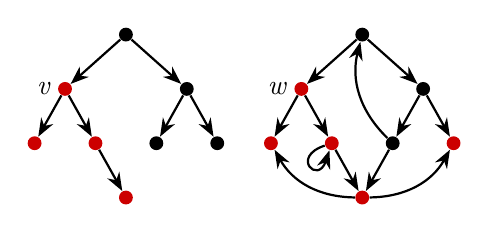
\begin{tikzpicture}[
  gnode/.style={circle, inner sep=0pt, minimum size=5pt, fill=black},
  gnodecol/.style={circle, inner sep=0pt, minimum size=5pt, fill=red},
  ->/.style={-Stealth, thick}, node distance=0.5cm]
  \node[gnode] (n0) {};
  \node[gnodecol] (n1) [below = of n0, xshift=-22pt] {};
  \node [left = of n1, xshift = 16pt] {$\m{v}$};
  \node[gnode] (n2) [below = of n0, xshift=22pt] {};
  \node[gnodecol] (n3) [below = of n1, xshift=-11pt] {};
  \node[gnodecol] (n4) [below = of n1, xshift=11pt] {};
  \node[gnode] (n5) [below = of n2, xshift=-11pt] {};
  \node[gnode] (n6) [below = of n2, xshift=11pt] {};
  \node[gnodecol] (n7) [below = of n4, xshift=11pt] {};
  \draw[->] (n0) to (n1);
  \draw[->] (n0) to (n2);
  \draw[->] (n1) to (n3);
  \draw[->] (n1) to (n4);
  \draw[->] (n2) to (n5);
  \draw[->] (n2) to (n6);
  \draw[->] (n4) to (n7);
  \node[gnode] (m0) [right = 80pt of n0]{};
  \node[gnodecol] (m1) [below = of m0, xshift=-22pt] {};
  \node [left = of m1, xshift = 16pt] {$\m{w}$};
  \node[gnode] (m2) [below = of m0, xshift=22pt] {};
  \node[gnodecol] (m3) [below = of m1, xshift=-11pt] {};
  \node[gnodecol] (m4) [below = of m1, xshift=11pt] {};
  \node[gnode] (m5) [below = of m2, xshift=-11pt] {};
  \node[gnodecol] (m6) [below = of m2, xshift=11pt] {};
  \node[gnodecol] (m7) [below = of m4, xshift=11pt] {};
  \draw[->] (m0) to (m1);
  \draw[->] (m0) to (m2);
  \draw[->] (m1) to (m3);
  \draw[->] (m1) to (m4);
  \draw[->] (m2) to (m5);
  \draw[->] (m2) to (m6);
  \draw[->] (m4) to (m7);
  \draw[->] (m5) to (m7);
  \draw[->] (m5) to [bend left] (m0);
  \draw[->] (m4) .. controls ([xshift=-15pt, yshift=-5pt] m4) and ([xshift=-5pt, yshift=-15pt] m4) .. (m4);
  \draw[->] (m7) to [bend right] (m6);
  \draw[->] (m7) to [bend left] (m3);
\end{tikzpicture}
   \captionof{figure}{A Binary Tree and a Binary Graph}
  \label{fig:bin_tree_graph}
\end{minipage}\begin{minipage}{.5\textwidth}
  \centering
  \vspace*{0.5em}
  \begin{tabular}[b]{c|c}
\textrm{\DIFaddFL{address}} & \textrm{\DIFaddFL{value}} \\
\hline
\DIFaddFL{102 }& \DIFaddFL{0 }\\
\DIFaddFL{101 }& \DIFaddFL{100 }\\
\DIFaddFL{100 }& \DIFaddFL{42 }\\
\end{tabular}
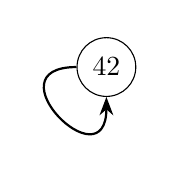
\begin{tikzpicture}
[->/.style={thick,arrows={-Stealth}},
   propG/.style={shape=circle, draw}]
   \path[use as bounding box] (-1, -1) rectangle (0.5, 0.5);
   \node[propG] (P) at (0, 0) {42};
   \draw[->] (P.west) .. controls (-1.5, 0) and (0, -1.5) .. (P.south);
\end{tikzpicture}
   \vspace*{1em}
  \captionof{figure}{A One-Cell Graph and its Heap Layout}
  \label{fig:single:cell}
\end{minipage}
\end{figure}

\DIFaddend \subsection{\texorpdfstring{Recursive \DIFdelbegin \DIFdel{definitions yield poor }\DIFdelend \DIFaddbegin \DIFadd{Definitions Yield Poor }\DIFaddend \p{graph} \DIFdelbegin \DIFdel{predicates}\DIFdelend \DIFaddbegin \DIFadd{Predicates}\DIFaddend}{XXX} }\label{sec:fixpointfail}

\newcommand{\graphkt}{\p{graph}_T}
\newcommand{\grapham}{\p{graph}_A}


Recursive predicates are ubiquitous in separation logic---so
much so that when one writes the definition of a predicate as
\mbox{$P$ ``$\defeq$'' $\ldots P \! \ldots$}, no one raises an eyebrow despite the
dangers of circularity in mathematics. Indeed, the vast majority of the time there
is no danger thanks to the magic of the Knaster-Tarski fixpoint
$\mu_{\mathsf{T}}$ \cite{tarski:fixpoint}.  Formally, one does not define $P$ directly,
but rather defines a functional
\mbox{$F_P \defeq \lambda P.~ \ldots P \! \ldots$} and then defines $P$ itself as
\mbox{$P \defeq \mu_{\mathsf{T}} \, F_P$}.
Assuming, as one typically does without comment,
that $F_P$ is \emph{covariant}, i.e. \DIFdelbegin \DIFdel{$(P \vdash Q)
\Rightarrow (F \, P \vdash F \, Q)$}\DIFdelend \DIFaddbegin \DIFadd{$(P |- Q)
\Rightarrow (F \, P |- F \, Q)$}\DIFaddend , one then enjoys the fixpoint
equation $P \Leftrightarrow \ldots P \ldots$, formally justifying
the typically-written pseudodefinition (``$\defeq$'').



Suppose we define a graph predicate $\graphkt$ \DIFdelbegin \DIFdel{this way, }\emph{\DIFdel{e.g.}} %DIFAUXCMD
\DIFdelend along the lines of the fold/unfold definition in Figure~\ref{fig:markgraph}\DIFaddbegin \DIFadd{.  Such a definition would use the overlapping conjunction $P ** Q$ (}\emph{\DIFadd{c.f.}} \DIFadd{Figure~\ref{fig:seplogsem}) as follows}\DIFaddend : \vspace{-1ex}
\[
\DIFdelbegin %DIFDELCMD < \begin{array}{@{}l@{}l@{}}
%DIFDELCMD < \graphkt(x, \gamma) \stackrel{\Delta}{=} \; &\Big(x = 0 /| \p{emp}\Big) |/ \\
%DIFDELCMD < &\quad \Big(\exists m,l,r.~ \gamma(x)=(m,l,r) /|
%DIFDELCMD < \big(x |-> m,l,r ** \graphkt(l, \gamma) ** \graphkt(r, \gamma)\big)\Big)
%DIFDELCMD < \end{array}
%DIFDELCMD < %%%
\DIFdelend \DIFaddbegin \begin{array}{@{}l@{}l@{}}
\graphkt(x, \gamma) \; \defeq \; &\Big(x = 0 /| \p{emp}\Big) |/ \\
&\quad \Big(\exists m,l,r.~ \gamma(x)=(m,l,r) /|
\big(x |-> m,l,r ** \graphkt(l, \gamma) ** \graphkt(r, \gamma)\big)\Big)
\end{array}
\DIFaddend \vspace{-1ex}
\]
Although we can apply Knaster-Tarski (because the functional needed to
define $\graphkt$ is covariant), the result is hard to use.
Consider the \DIFdelbegin \DIFdel{following }\DIFdelend memory $m$ for a toy machine\DIFdelbegin \DIFdel{:
}%DIFDELCMD < 

%DIFDELCMD < \begin{wrapfigure}{r}{.39\textwidth}
%DIFDELCMD < \vspace{-2em} \begin{minipage}{.20\textwidth}
%DIFDELCMD < \qquad %%%
\[
\DIFdel{\begin{array}{c|c}
\textrm{address} & \textrm{value} \\
\hline
102 & 0 \\
101 & 100 \\
100 & 42 \\
\end{array}
}\]
%DIFAUXCMD
%DIFDELCMD < \end{minipage}
%DIFDELCMD < \begin{minipage}{.19\textwidth}
%DIFDELCMD < \centering
%DIFDELCMD < %%%
%DIF <  \beginpgfgraphicnamed{selfref}
%DIFDELCMD < \begin{tikzpicture}
%DIFDELCMD < [->/.style={thick,arrows={-Stealth}},
%DIFDELCMD <    propG/.style={shape=circle, draw}]
%DIFDELCMD <    \path[use as bounding box] (-1, -1) rectangle (0.5, 0.5);
%DIFDELCMD <    \node[propG] (P) at (0, 0) {42};
%DIFDELCMD <    \draw[->] (P.west) .. controls (-1.5, 0) and (0, -1.5) .. (P.south);
%DIFDELCMD < \end{tikzpicture}
%DIFDELCMD < %%%
%DIF <  \endpgfgraphicnamed
%DIFDELCMD < \end{minipage}
%DIFDELCMD < \vspace{-0.5em} \end{wrapfigure}
%DIFDELCMD < 

%DIFDELCMD < \noindent %%%
\DIFdel{Clearly }\DIFdelend \DIFaddbegin \DIFadd{, where }\DIFaddend $m |= 100 |-> 42,100,0$.
\DIFdelbegin \DIFdel{But it seems also clear}\DIFdelend \DIFaddbegin \DIFadd{It seems clear, however, }\DIFaddend that this
memory \DIFaddbegin \DIFadd{also }\DIFaddend represents a one-cell cyclic graph as illustrated in
\DIFdelbegin \DIFdel{the accompanying diagram}\DIFdelend \DIFaddbegin \DIFadd{Figure~\ref{fig:single:cell}}\DIFaddend , \emph{i.e.} we want
$m |= \graphkt(100,\hat{\gamma})$, where 
$\hat{\gamma}(100) = (42,100,0)$.  This is equivalent to wanting to be able to 
prove $100~|->~42,100,0~|-~\graphkt(100,\hat{\gamma})$.  Unfortunately, as 
\DIFdelbegin \DIFdel{explained in Appendix~C}%DIFDELCMD < \hide{\ref{apx:problemrecgraph}}%%%
\DIFdelend \DIFaddbegin \DIFadd{illustrated in Figure~\ref{fig:badcycle}}\DIFaddend , this is rather difficult to do since 
applying the natural proof techniques actually strengthens the goal.
\DIFdelbegin \DIFdel{In fact we }\DIFdelend \DIFaddbegin \DIFadd{Part of the 
problem is that the recursive structure interacts very badly with $**$: if the 
recursion involved~$*$~then it }\textbf{\DIFadd{would}} \DIFadd{be provable, by induction on the 
finite memory (each ``recursive call'' would be on a strictly smaller subheap).  
This is why Knaster-Tarski works so well with list, tree, and DAG predicates in 
separation logic.  We }\DIFaddend do not know if this entailment is provable, but the 
difficulties encountered in proving what ``should be'' straightforward suggest 
that Knaster-Tarski should be treated with caution when defining spatial 
predicates for graphs.

\DIFaddbegin \begin{figure}[htbp]
\[
\infrule{}
{\infrule{}
 {\DIFaddFL{100 |-> 42,100,0 ~ |- ~ 100 |-> 42,100,0 ** \graphkt(100,\hat{\gamma})}}
  {\DIFaddFL{100 |-> 42,100,0 ~ |- ~ \hat{\gamma}(100) = (42,100,0) ~ /| ~ 100 |-> 42,100,0 ** \graphkt(100,\hat{\gamma}) ** \graphkt(0,\hat{\gamma})}}
  {\DIFaddFL{\ddagger}}
}
{\DIFaddFL{100 |-> 42,100,0 ~ |- ~ \graphkt(100,\hat{\gamma})}}
{\DIFaddFL{\dagger}}
\]x
\begin{tabular}{@{}l@{$~~$}l|l@{$~~$}l}
\DIFaddFL{$\dagger$ }& \DIFaddFL{Unfold $\graphkt$, dismiss first disjunct (contradiction), $~~$ }& \DIFaddFL{$~~$ $\ddagger$ }&\DIFaddFL{simplify using $P * \p{emp} -|- P$ }\\
& \DIFaddFL{introduce existentials (which must be 42,100,0) }& & \DIFaddFL{and remove pure conjunct
}\end{tabular}
\caption{\DIFaddFL{An attempt to prove a ``simple'' entailment}}
\label{fig:badcycle}
\end{figure}


\DIFaddend The other direction, \mbox{$\graphkt(100,\hat{\gamma}) |- 100 |-> 42,100,0$},
\textbf{is} true but is not easy to prove, relying on the constructions in \S\ref{sec:goodgraph} and the fact that $\mu_{\mathsf{T}}$ constructs the least fixpoint.  In contrast, $\graphkt(100,\hat{\gamma}) |- 100 |-> 42,100,0 * \top$ is easy. 

\DIFaddbegin \hide{
\cite{appel:fixpoint} defined an alternative fixpoint using a notation of \emph{contractiveness}.  Unfortunately, this alternative fixpoint also
fails to define a sensible graph predicate; see Appendix~\ref{apx:appelfixpiont}.

\subsection{Problem with Appel and McAllester's fixpoint}
\label{apx:appelfixpiont} }

\DIFadd{Appel and McAllester proposed another fixpoint $\mu_{\mathsf{A}}$
that is sometimes used to define recursive predicates in separation
logic \mbox{%DIFAUXCMD
\cite{appel:fixpoint}}\hspace{0pt}%DIFAUXCMD
.  This time the functional $F_P$ needs to be
}\emph{\DIFadd{contractive}}\DIFadd{, which to a first order of approximation means that
all recursion needs to be guarded by~$\rhd$~, the ``approximation
modality'' \mbox{%DIFAUXCMD
\cite{appel:vmm}}\hspace{0pt}%DIFAUXCMD
, }\emph{\DIFadd{i.e.}} \DIFadd{our graph predicate would
look like
}\begin{align*}
\DIFadd{\grapham(x, \gamma) ~ \defeq ~~ }&\DIFadd{(x = 0 /| \p{emp}) |/ \exists m,l,r.~ \gamma(x)=(m,l,r) /| \null }\\
 & \DIFadd{x |-> m,l,r ** \rhd \grapham(l, \gamma) ** \rhd \grapham(r, \gamma)
}\end{align*}
\DIFadd{This functional is contractive, and so the fixpoint is well-defined.  
Nevertheless, this definition has a subtle flaw: the resulting graph
predicate is }\textbf{\DIFadd{not}} \DIFadd{``precise'' in the separation logic sense:
}\[
\DIFadd{\m{precise}(P) ~~ \defeq ~~ (\sigma_1 |= P) ~ => ~ (\sigma_2 |= P) ~ => ~ (\sigma_1 \oplus \sigma_1' \! = \! \sigma) ~ => ~ (\sigma_2 \oplus \sigma_2' \! = \! \sigma) ~ => ~ \sigma_1 \! = \! \sigma_2
}\]
\DIFadd{The flaw stems from the fact that $\rhd P$ is not precise for any $P$ 
(at time zero, $\rhd P$ is just $\top$), 
so $\grapham$ is not precise either.  The approximation modality's 
universal imprecision has never been noticed before in the literature.
Accordingly, $\grapham$ is also rather difficult to use.
}


\hide{
\section{Difficulty using $\graphkt$}
\label{apx:problemrecgraph}


See Figure \ref{fig:badcycle} for an attempt to prove the entailment $100 |-> 42,100,0 ~ |- ~ \graphkt(100,\hat{\gamma})$.  Part of the problem is that the recursive structure interacts very badly with $**$: if the recursion involved~$*$~then it \textbf{would} be provable, by induction on the finite memory (each ``recursive call'' would be on a strictly smaller subheap).  This is why Knaster-Tarski works so well with list, tree, and DAG predicates in separation logic.
}












\DIFaddend \subsection{\texorpdfstring{Defining a \DIFdelbegin \DIFdel{good }\DIFdelend \DIFaddbegin \DIFadd{Good }\DIFaddend \p{graph} \DIFdelbegin \DIFdel{predicate}\DIFdelend \DIFaddbegin \DIFadd{Predicate}\DIFaddend}{XXX} }\label{sec:goodgraph}

Rather than trying to define \p{graph} as a recursive fixpoint,
we will instead give it a flat structure.  Graphs in separation
logic have been defined in similar ways before, \emph{e.g.}~\DIFdelbegin \DIFdel{\mbox{%DIFAUXCMD
\cite{ilya-graphs}}\hspace{0pt}%DIFAUXCMD
}\DIFdelend \DIFaddbegin \DIFadd{\mbox{%DIFAUXCMD
\citet{ilya-graphs}}\hspace{0pt}%DIFAUXCMD
}\DIFaddend ;
our innovation is that we prove---with the amount of precision
required to convince Coq---that we can still enjoy fold/unfold
with our flat definition.  Our path starts with the iterated
separating conjunction or ``big star'', which is first defined over
lists and then extended to sets as follows:

\vspace{-1em}
\[
\DIFdelbegin %DIFDELCMD < \begin{array}{@{}l@{}}
%DIFDELCMD < \underset{\{l_1, l_2,\dots,l_n\}}{\bigstar}P ~~ \defeq ~~ P(l_1) *
%DIFDELCMD <   P(l_2) * \dots * P(l_n) \quad \vline \quad
%DIFDELCMD < \underset{S}{\bigstar} P ~~ \defeq ~~ \exists L.~ (\p{NoDup}\ L) /| (\forall x.~ x\ \p{in}\ L <=> x \in S) /| \underset{L}{\bigstar}P
%DIFDELCMD < \end{array}
%DIFDELCMD < %%%
\DIFdelend \DIFaddbegin \begin{array}{@{}l@{}}
\!\!\!\!\!\!\!\underset{\{l_1,\dots,l_n\}}{\bigstar P}\!\!\!\!\!\!\! ~~ \defeq ~~ P(l_1) *
  P(l_2) * \dots * P(l_n) \quad \vline \quad
\underset{S}{\bigstar} P ~~ \defeq ~~ \exists L.~ (\p{NoDup}\ L) /| (\forall x.~ x\ \p{in}\ L <=> x \in S) /| \underset{L}{\bigstar}P
\end{array}
\DIFaddend \]

We are now ready to define a good \p{graph} predicate:
  \quad \DIFdelbegin \DIFdel{$\p{graph}(x, \gamma) \; \defeq \; \underset{v \in \mathit{reach}(\gamma, x)}{\bigstar} v\mapsto\gamma(v)$
}\DIFdelend 

\DIFaddbegin \DIFadd{$\p{graph}(x, \gamma) \; \defeq \; \!\!\!\!\!\!\!\!\!\!\underset{\m{v} \in \mathit{reachable}(\gamma, x)}{\bigstar}\!\!\!\!\!\!\m{v}\mapsto\gamma(\m{v})$.
}\DIFaddend \iffalse
\begin{equation*}
  \underset{\{l_1, l_2,\dots,l_n\}}{\bigstar}P ~~ \defeq ~~ P(l_1) *
  P(l_2) * \dots * P(l_n).
\end{equation*}
Formally $\bigstar$ is defined over a list rather than a set and is parameterized by a predicate $P$.  It is natural to extend $\bigstar$ to a set $S$ with an existentially-quantified duplicate-free list~$L$:
\[
\underset{S}{\bigstar} P ~~ \defeq ~~ \exists L.~ (\p{NoDup}\ L) /| (\forall x.~ x\ \p{in}\ L <=> x \in S) /| \underset{L}{\bigstar}P
\]
We use the same $\bigstar$ notation since the concepts are similar, but the existential adds a little pain since we need to prove that all choices of $L$ yield equivalent predicates.

We are now ready to give a good \p{graph} predicate:
\fi


\hide{ \vspace{-1.5ex}
\begin{equation}\label{eqn:iter_def}
  \p{graph}(x, \gamma) ~~ \defeq ~~ \underset{v \in \mathit{reach}(\gamma, x)}{\bigstar} v\mapsto\gamma(v)
\vspace{-1.5ex}
\end{equation}
$\gamma$ is a GeneralGraph and ``$x |-> \gamma(x)$'' is a predicate that says how a single node fits in memory. In Figure~\ref{fig:markgraph} it was:
\[
\exists m,l,r.~\gamma(x) = (m,l,r) /| x |-> m,-,l,r /| x\ \p{mod}\ 16 = 0
\]}
The graph $\gamma$ here need not be a bigraph, but \emph{e.g.} can have many edges.

Our definition of \p{graph} is flat in the sense that there is no obvious way to follow the link structure recursively.  Happily, we can recover a general recursive fold/unfold (if $x |-> \gamma(x)$ and the GeneralGraph has the necessary properties in its soundness condition):
\vspace{-1ex}
\begin{equation}
\label{eqn:unfold_graph}
\hspace{-1em}\DIFdelbegin %DIFDELCMD < \begin{array}{@{}lc@{\hspace{1pt}}c@{\hspace{1pt}}l@{}}
%DIFDELCMD < \p{graph}(x,\gamma)  <=>  x |-> \gamma(x) ** \big(\!\!\!\!\!\!\!\!\!\!\!\!\!\underset{n \in \p{neighbors}(\gamma,x)}{\raisebox{-0.3ex}{\resizebox{0.75em}{!}{$\scon$}} \hspace{-2.18ex} \bigcup}\!\!\!\!\!\!\!\!\!\!\!\! \p{graph}(\gamma,n) \big)
%DIFDELCMD < \quad \text{~~~ where ~~ }\underset{l_1,\dots,l_n}{\raisebox{-0.3ex}{\resizebox{0.75em}{!}{$\scon$}}\hspace{-2.18ex} \bigcup} \! \! P  \defeq  P(l_1) ** \ldots ** P(l_n) \end{array}
%DIFDELCMD < %%%
\DIFdelend \DIFaddbegin \begin{array}{@{}lc@{\hspace{1pt}}c@{\hspace{1pt}}l@{}}
\p{graph}(x,\gamma)  <=>  x |-> \gamma(x) ** \big(\!\!\!\!\!\!\!\!\!\!\!\!\!\underset{n \in \p{neighbors}(\gamma,x)}{\bigocon}\!\!\!\!\!\!\!\!\!\!\!\! \p{graph}(\gamma,n) \big)
\quad \text{~~~ where ~~ }\underset{l_1,\dots,l_n}{\raisebox{-0.3ex}{\resizebox{0.75em}{!}{\hspace{0.05em}$\scon$}}\hspace{-2.18ex} \bigcup} \! \! P  \defeq  P(l_1) ** \ldots ** P(l_n) \end{array}
\DIFaddend \vspace{-1ex}
\end{equation}

The proof of the $<=$ direction requires care. The difficulty is that if two nodes $x |-> \gamma(x)$ and $x' |-> \gamma(x')$ are \emph{skewed}, \emph{i.e.} ``partially overlapping'' with some---but not all---of $x$'s memory cells shared with $x'$, then the $\bigstar$ on the left hand side cannot separate them.  To avoid skewing we require that $x |-> \gamma(x)$ be \emph{alignable}. A predicate $P$ is alignable when
\[
\forall x,y.~ \Big(P(x) ** P(y) |- \big(P(x) /| x = y\big) |/ \big(P(x) * P(y)\big)\Big)
\]
That is, they overlap either completely or not at all. In a Java-like memory model this property is automatic because pointers in such a model always point to the root/beginning of an object.  In contrast, in a C-like memory model such as in VST/CompCert, this property is not automatic because pointers can point anywhere.  In such a model, alignment is most easily enforced by storing graph nodes at addresses that are multiples of an appropriate size (\DIFdelbegin \DIFdel{16 }\DIFdelend \DIFaddbegin \emph{\DIFadd{e.g}} \DIFadd{this size is $16$ }\DIFaddend in Figure~\ref{fig:markgraph}).

Some of our VST proofs, \emph{e.g.} for \DIFdelbegin \texttt{\DIFdel{find}}%DIFAUXCMD
\DIFdelend \DIFaddbegin \li{find}\DIFaddend , do not use fold/unfold, instead preferring to use the lemmas in~\S\ref{sec:ramifylib} directly.  Others, \emph{e.g.} \DIFdelbegin \texttt{\DIFdel{mark}}%DIFAUXCMD
\DIFdel{, do---and }\DIFdelend \DIFaddbegin \li{mark}\DIFadd{, do, and }\DIFaddend it is helpful to have both options avilable. We also prove fold/unfold lemma for DAGs in which we get a \DIFaddbegin \DIFadd{clean }\DIFaddend $*$ between the root and its $**$-joined neighbors, rather than the $**$ present in \eqref{eqn:unfold_graph}.



\subsection{Ramification Libraries}\label{sec:ramifylib}

\begin{figure}
\centering
%DIF <  \beginpgfgraphicnamed{infrastructure}
\DIFdelbeginFL %DIFDELCMD < \begin{tikzpicture}[
%DIFDELCMD < ->/.style={thick, arrows={-Stealth}},
%DIFDELCMD < ent/.style={shape=rectangle, rounded corners=4pt, draw, on grid},x=33pt]
%DIFDELCMD < \node[ent] (SM) at (0, 0) {\small Step-Indexed Model};
%DIFDELCMD < \node[ent] (DM) [right=4.4 of SM] {\small Direct Model};
%DIFDELCMD < \node[ent] (CL) [above=1 of SM] {\small Core Logic};
%DIFDELCMD < \node[ent] (SL) [above=1 of DM] {\small Supplementary Logic};
%DIFDELCMD < \node[ent] (LF) [above left=1 and 1.2 of CL] {\small Logic Facts};
%DIFDELCMD < \node[ent] (RF) [above right=1 and 1.2 of CL] {\small Basic Ramification};
%DIFDELCMD < \node[ent] (BF) [above=1 of LF] {\small $\bigstar$ Facts};
%DIFDELCMD < \node[ent] (BR) [above=1 of RF] {\small $\bigstar$ Ramification};
%DIFDELCMD < \node[ent] (GF) [above=1 of BF] {\small Graph Facts};
%DIFDELCMD < \node[ent] (GR) [above=1 of BR] {\small Graph Ramification};
%DIFDELCMD < \node[ent] (SLF) [above=1 of SL] {\small Supplementary Logic Facts};
%DIFDELCMD < \node[ent] (SBF) [above=1 of SLF] {\small Supplementary $\bigstar$ Facts};
%DIFDELCMD < \node[ent] (SGF) [above=1 of SBF] {\small Supplementary Graph Facts};
%DIFDELCMD < \draw [double, ->] (SM) to (CL);
%DIFDELCMD < \draw [double, ->] (SM) to (SL);
%DIFDELCMD < \draw [double, ->] (DM) to (CL);
%DIFDELCMD < \draw [double, ->] (DM) to (SL);
%DIFDELCMD < \draw [->] (CL) to (LF);
%DIFDELCMD < \draw [->] (CL) to (RF);
%DIFDELCMD < \draw [->] (CL) to (SL);
%DIFDELCMD < \draw [->] (SL) to (SLF);
%DIFDELCMD < \draw [->] (SLF) to (SBF);
%DIFDELCMD < \draw [->] (SBF) to (SGF);
%DIFDELCMD < \draw [->] (LF) to (RF);
%DIFDELCMD < \draw [->] (LF) to (BF);
%DIFDELCMD < \draw [->] (RF) to (SLF);
%DIFDELCMD < \draw [->] (RF) to (BR);
%DIFDELCMD < \draw [->] (BF) to (BR);
%DIFDELCMD < \draw [->] (BF) to (GF);
%DIFDELCMD < \draw [->] (GF) to (GR);
%DIFDELCMD < \draw [->] (GR) to (SGF);
%DIFDELCMD < \draw [->] (BR) to (GR);
%DIFDELCMD < \draw [->] (BR) to (SBF);
%DIFDELCMD < \node (legend1) [below right=0.2 and -1.2 of SM] {\small Dependence};
%DIFDELCMD < \coordinate[left=0.8 of legend1]  (l1);
%DIFDELCMD < \draw [->] (l1) to (legend1);
%DIFDELCMD < \node (legend2) [right=1 of legend1] {\small Instantialization Choices};
%DIFDELCMD < \coordinate[left=0.8 of legend2]  (l2);
%DIFDELCMD < \draw [double, ->] (l2) to (legend2);
%DIFDELCMD < \end{tikzpicture}
%DIFDELCMD < %%%
%DIF <  \endpgfgraphicnamed
\DIFdelendFL \DIFaddbeginFL \begin{adjustbox}{scale=0.80}
\begin{tikzpicture}[
->/.style={thick, arrows={-Stealth}},
ent/.style={shape=rectangle, rounded corners=4pt, draw, on grid},
entcol/.style={shape=rectangle, rounded corners=4pt, draw, on grid, fill=red!30},x=33pt]
\node[ent] (SM) at (0, 0) {\small Step-Indexed Model};
\node[ent] (DM) [right=4.9 of SM] {\small Direct Model};
\node[entcol] (CL) [above=1.5 of SM] {\small Core Logic Interface};
\node[ent] (SL) [above=1.5 of DM] {\small Supplementary Logic Interface};
\node[entcol] (LF) [above left=1 and 1.2 of CL] {\small Logic Facts};
\node[entcol] (RF) [above right=1 and 1.2 of CL] {\small Basic Ramification};
\node[entcol] (BF) [above=1 of LF] {{\scriptsize $\bigstar$} {\small Facts}};
\node[entcol] (BR) [above=1 of RF] {{\scriptsize $\bigstar$} {\small Ramification}};
\node[entcol] (GF) [above=1 of BF] {\small Graph Facts};
\node[entcol] (GR) [above=1 of BR] {\small Graph Ramification};
\node[ent] (SLF) [above=1 of SL] {\small Supplementary Logic Facts};
\node[ent] (SBF) [above=1 of SLF] {\small Supplementary {\scriptsize $\bigstar$} Facts};
\node[ent] (SGF) [above=1 of SBF] {\small Supplementary Graph Facts};
\draw [double, ->] (SM) to (CL);
\draw [double, ->] (SM) to [bend right=12] (SL);
\draw [double, ->] (DM) to [bend left=12] (CL);
\draw [double, ->] (DM) to (SL);
\draw [->] (CL) to (LF);
\draw [->] (CL) to (RF);
\draw [->] (CL) to (SL);
\draw [->] (SL) to (SLF);
\draw [->] (SLF) to (SBF);
\draw [->] (SBF) to (SGF);
\draw [->] (LF) to (RF);
\draw [->] (LF) to (BF);
\draw [->] (RF) to (SLF);
\draw [->] (RF) to (BR);
\draw [->] (BF) to (BR);
\draw [->] (BF) to (GF);
\draw [->] (GF) to (GR);
\draw [->] (GR) to (SGF);
\draw [->] (BR) to (GR);
\draw [->] (BR) to (SBF);
\node (legend1) [below right=0.2 and -1.2 of SM] {\small Dependence};
\coordinate[left=0.8 of legend1]  (l1);
\draw [->] (l1) to (legend1);
\node (legend2) [right=1 of legend1] {\small Instantialization Options};
\coordinate[left=0.8 of legend2]  (l2);
\draw [double, ->] (l2) to (legend2);
\end{tikzpicture}
\end{adjustbox}
\DIFaddendFL \caption{Infrastructure of ramification library}\label{fig:infra}
\end{figure}
%DIF > 


\DIFdelbegin \DIFdel{VST employs a somewhat unusual }\DIFdelend \DIFaddbegin \DIFadd{Many tools (}\emph{\DIFadd{e.g.}}\DIFadd{\ Charge! \mbox{%DIFAUXCMD
\citep{bengtson:charge}}\hspace{0pt}%DIFAUXCMD
,
Smallfoot \mbox{%DIFAUXCMD
\citep{berdine:smallfoot}}\hspace{0pt}%DIFAUXCMD
, jStar \mbox{%DIFAUXCMD
\citep{distefanop08}}\hspace{0pt}%DIFAUXCMD
,
HIP/SLEEK \mbox{%DIFAUXCMD
\citep{chin:hipsleek}}\hspace{0pt}%DIFAUXCMD
) use the Direct Model to represent
spatial predicates on the heap, but VST employs an unusually complex
}\DIFaddend Step-Indexed heap model \DIFdelbegin \DIFdel{to represent
spatial predicates, and uses it to }\DIFdelend \DIFaddbegin \DIFadd{in order to }\DIFaddend support an unusually rich program
logic\DIFdelbegin \DIFdel{.~\mbox{%DIFAUXCMD
\cite{appel:programlogics}}\hspace{0pt}%DIFAUXCMD
However, the
spatial representation
of our graph library does }\DIFdelend \DIFaddbegin \DIFadd{~\mbox{%DIFAUXCMD
\cite{appel:programlogics}}\hspace{0pt}%DIFAUXCMD
.  Figure~\ref{fig:infra} shows the
architecture of our spatial development.  We will explain our two
interfaces momentarily, but for now observe that both heap models can
instantiate both interfaces. That is to say, we do }\DIFaddend not rely on any of \DIFdelbegin \DIFdel{its bellsand whistles.
To isolate our development from these unnecessary complications,
we use }\DIFdelend \DIFaddbegin \DIFadd{the
bells, whistles, or specialized properties that are only available 
in the Step-Indexed Model.
}

\DIFadd{We modularize our spatial library over 
}\DIFaddend two interfaces: Core Logic and Supplementary Logic\DIFdelbegin \DIFdel{, where Supplementary Logic is built upon the much simpler
and more universal Direct Model of heap representation.
We present the architecture of our spatial development in
Figure~\ref{fig:infra}, where it should be straighforward to see
that both models can instantiate both interfaces.
}%DIFDELCMD < 

%DIFDELCMD < %%%
\DIFdel{Generally speaking, our VST proofs only need the Core properties to prove
our examples. }\DIFdelend \DIFaddbegin \DIFadd{.
}\DIFaddend Each interface defines some operators of separation logic 
\DIFdelbegin \DIFdel{and
provides some axioms about }\DIFdelend \DIFaddbegin \DIFadd{along with relevant axioms to show }\DIFaddend how they work.  
For example, \DIFaddbegin \DIFadd{the definitions of }\DIFaddend $*$ and
$--*$ are in Core Logic, along with \DIFdelbegin \DIFdel{the axiom
}\DIFdelend \DIFaddbegin \DIFadd{key axioms and rules such as
}\DIFaddend $(P |- Q --* R) <=> (P * Q |- R)$.  
On the other hand, \DIFdelbegin \DIFdel{the }\DIFdelend \DIFaddbegin \DIFadd{lesser-used operators such as 
}\DIFaddend $**$ and $--o$ \DIFdelbegin \DIFdel{operators }\DIFdelend are in Supplementary Logic,
along with rules \DIFdelbegin \DIFdel{like }\DIFdelend \DIFaddbegin \DIFadd{such as }\DIFaddend $P |- P ** P$. 
\DIFaddbegin \DIFadd{Generally speaking, our VST proofs only need Core properties 
(shaded in the figure) to prove our examples.
}\DIFaddend 

\hide{Starting from the bottom, notice that there are two underlying heap models,
VST's Step-Indexed model and the much simpler Direct Model.

To isolate our development from these unnecessary complications,
{\color{magenta}and to ensure that HIP/SLEEK can reuse our spatial
reasoning, we use two interfaces: Core Logic and Supplementary
Logic.  Both models can instantiate both interfaces, but generally
speaking our VST proofs only need the Core properties to prove
our examples, whereas HIP/SLEEK uses both Core and Supplemental.}
Each interface defines some operators of separation logic and
provides some axioms about how they work.  For example, $*$ and
$--*$ are in Core Logic, along with the axiom
$(P |- Q --* R) <=> (P * Q |- R)$.  On the other hand,
the $**$ and $--o$ operators are in Supplementary Logic,
along with rules like $P |- P ** P$.} 

Above the Logic layer we have three towers, each three levels high.  The tower on the left contains basic lemmas about Logic, $\bigstar$, and \p{graph}.  For instance, in the $\bigstar$ Facts box we prove:
\DIFdelbegin \[
\infrule{}
{\DIFdel{A \cap B = \emptyset}}
{\DIFdel{\underset{x\in A}{\bigstar} P(x) \; * \underset{x\in B}{\bigstar} P(x) \;\, \Leftrightarrow \underset{x\in A \cup B}{\bigstar} P(x)}}{}
\]
%DIFAUXCMD
%DIFDELCMD < 

%DIFDELCMD < %%%
\DIFdelend \DIFaddbegin \begin{equation*}
\infrule{}
{\DIFadd{A \cap B = \emptyset}}
{\DIFadd{\underset{x\in A}{\bigstar} P(x) \; * \underset{x\in B}{\bigstar} P(x) \;\, \Leftrightarrow \underset{x\in A \cup B}{\bigstar} P(x)}}{}
\end{equation*}
\DIFaddend The middle tower is more interesting in that it is entirely focused on ramification entailments.  A robust library of ramification entailments is essential to make ramification work smoothly in practice.  The Basic Ramification box in the lower layer contains lemmas like \DIFdelbegin \DIFdel{:
}\[
\infrule{}
{\DIFdel{G_1 \vdash L_1 * \forall x.~ (L_2 --* G_2) }\\
 \DIFdel{G'_1 \vdash L'_1 * \forall x.~ (L_2' --* G'_2)}}
{\DIFdel{G_1 * G'_1 \vdash (L_1 * L'_1) * \forall x.~ \big((L_2 * L'_2)--* (G_2 * G'_2)\big)}}{}
\]
%DIFAUXCMD
\DIFdel{We use this lemma }\DIFdelend \DIFaddbegin \DIFadd{the one below, which we use }\DIFaddend to break large ramification entailments into \DIFdelbegin \DIFdel{more manageable piecesin a compositional way. }\DIFdelend \DIFaddbegin \DIFadd{compositionally manageable pieces. }\begin{equation*}
\infrule{}
{\DIFadd{G_1 |- L_1 * \forall x.~ (L_2 --* G_2) }\\
 \DIFadd{G'_1 |- L'_1 * \forall x.~ (L_2' --* G'_2)}}
{\DIFadd{G_1 * G'_1 |- (L_1 * L'_1) * \forall x.~ \big((L_2 * L'_2)--* (G_2 * G'_2)\big)}}{}
\end{equation*}
\DIFaddend The $\bigstar$ Ramification box in the middle layer contains lemmas like \DIFdelbegin \DIFdel{:
}\DIFdelend \DIFaddbegin \DIFadd{the one below:
}\DIFaddend \begin{equation*}
\DIFdelbegin %DIFDELCMD < \label{ramify:bigstar}
%DIFDELCMD < %%%
\DIFdelend \infrule{}
{A \cap B = \emptyset  \qquad  A' \cap B = \emptyset}
{\underset{x\in A\cup B}{\bigstar} P(x) \DIFdelbegin \DIFdel{\vdash }\DIFdelend \DIFaddbegin \DIFadd{|- }\DIFaddend \! \underset{x\in A}{\bigstar} \! P(x) * \Big( \underset{x\in A'}{\bigstar} \! P(x) \! \wand \! \! \! \! \underset{x\in A' \cup B}{\bigstar} \! \! P(x)\Big)}{}
\DIFdelbegin %DIFDELCMD <
\end{equation*}
%DIFDELCMD < 

%DIFDELCMD < %%%
\DIFdel{The }\DIFdelend \DIFaddbegin
\DIFadd{The above lemma expresses large-scale replacement, clearing the way to 
cleanly establish a key graph-specific fact:
Lemma~\ref{ramify:bigstar}, which is 
placed in the }\DIFaddend Graph Ramification box \DIFdelbegin \DIFdel{in the top layeris focused lemmas such as the following ``update one node'' lemma , which was }\DIFdelend \DIFaddbegin \DIFadd{(top layer), is used on 
lines~\ref{code:markram3} and~\ref{code:markram4} of 
Figure~\ref{fig:markgraph} to reason about smoothly replacing subgraphs. 
}\begin{equation}
\DIFadd{\label{ramify:bigstar}
\frac{n \in \p{neighbors}(\gamma,x)}{
\p{graph}(x, \gamma) |- \p{graph}(n, \gamma) \! * \!
\forall \gamma'. \m{mark}(\gamma, n, \gamma') -> \big(\p{graph}(n, \gamma') \! --* \! \p{graph}(x, \gamma')\big)
}
}\end{equation}
\DIFadd{Similarily, the same box contains the key lemma }\DIFaddend used on line~\ref{code:markram2} in Figure~\ref{fig:markgraph} \DIFdelbegin \DIFdel{:
}\begin{displaymath}
\infrule{}
{\DIFdel{\forall x_0 \neq x.~ \gamma(x_0) = \gamma'(x_0) }\\ \DIFdel{\p{neighbors}(\gamma,x)=\p{neighbors}(\gamma',x)}}
{\DIFdel{\p{graph}(x, \gamma) \! \vdash \! x \! \mapsto \! \gamma(x) \! * \! \big(x \! \mapsto \! \gamma'(x) \! \wand \! \p{graph}(x, \gamma')\big)}}{}
\end{displaymath}
%DIFAUXCMD
%DIFDELCMD < 

%DIFDELCMD < %%%
\DIFdelend \DIFaddbegin \DIFadd{to update one node:
}\begin{equation}
\DIFadd{\label{lem:updategraphnode}
\frac{\forall x_0 \neq x.~ \gamma(x_0) = \gamma'(x_0) \\ \p{neighbors}(\gamma,x)=\p{neighbors}(\gamma',x)}{\p{graph}(x, \gamma) \! |- \! x \! \mapsto \! \gamma(x) \! * \! \big(x \! \mapsto \! \gamma'(x) \! \wand \! \p{graph}(x, \gamma')\big)}
}\end{equation}
\DIFaddend This layered structure enables proof reuse. All of the theorems for $\p{graph}$ are proved from the properties of iterated separating conjunction, but having a modular library allows $\bigstar$ to be reused in other structures smoothly.
Further, all our verifications of different graph algorithms use the proof rules of $\p{graph}$ at the top level in the library. 
\DIFdelbegin \DIFdel{Taking the marking algorithm we introduced in \S\ref{sec:orientation} as an example, we prove the following theorem from the library:
}\begin{displaymath}
\DIFdel{%DIFDELCMD < \label{lem:updatesubgraph}%%%
\frac{n \in \p{neighbors}(\gamma,x)}{
\mbox{
%
\mbox{%DIFAUXCMD
$\begin{array}{@{}l@{}l@{}}
\p{graph}(x, \gamma) \vdash \p{graph}(n, \gamma) \! * \!
\big(\forall \gamma'. \m{mark}(\gamma, n, \gamma') \! /| \! \p{graph}(n, \gamma') \! --*
\m{mark}(\gamma, n, \gamma') \! /| \! \p{graph}(x, \gamma')\big)
\end{array}$
}%DIFAUXCMD
}
}
}\end{displaymath}
%DIFAUXCMD
\DIFdelend 

\DIFaddbegin \hide{Taking the marking algorithm we introduced in \S\ref{sec:orientation} as an example, we prove the following theorem from the library:
{\color{red}
\begin{equation*}
\label{lem:updatesubgraph}
\frac{n \in \p{neighbors}(\gamma,x)}{
\p{graph}(x, \gamma) |- \p{graph}(n, \gamma) \! * \!
\forall \gamma'. \m{mark}(\gamma, n, \gamma') -> \big(\p{graph}(n, \gamma') \! --* \! \p{graph}(x, \gamma')\big)
}
\end{equation*}
}
}

\DIFaddend The Supplementary tower contains properties not used by most of the VST examples.
This includes the fold/unfold relationship \DIFdelbegin \DIFdel{from }\DIFdelend \DIFaddbegin \DIFadd{that we moved away from 
in~}\DIFaddend \S\ref{sec:goodgraph}, facts
about precision, \emph{etc}. These are currently included mostly for completeness,
but do make our library more general should we wish to accommodate an alternate
prover that \DIFdelbegin \DIFdel{uses the Direct Model.
}\DIFdelend \DIFaddbegin \DIFadd{needs separation logic facts about $**$,  $--o$, }\emph{\DIFadd{etc.}}
\DIFaddend 










 
\section{Certifying a Garbage Collector for CertiCoq}
\label{sec:certigc}


\hide{The GC is our most complicated example,
and we will discuss some of its key proofs, but the larger
point here is that we completed this certification using
exactly the framework and principles we have discussed
thus far.

We enjoyed significant code
reuse from our prior certifications, and when we stated
new lemmas for the GC, we filed them away at the appropriate
``layers'' so that they may be reused in the future.
}


\DIFdelbegin \subsection{\texorpdfstring{\DIFdel{Background}}{XXX}}
%DIFAUXCMD
\addtocounter{subsection}{-1}%DIFAUXCMD
%DIFDELCMD < \label{sec:gcbackground}
%DIFDELCMD < 

%DIFDELCMD < %%%
\DIFdelend The CertiCoq compiler \cite{certicoqpaper} translates Gallina code to
Clight, which CompCert\DIFaddbegin \DIFadd{~\mbox{%DIFAUXCMD
\cite{leroy:compcert} }\hspace{0pt}%DIFAUXCMD
then }\DIFaddend compiles to assembly\DIFdelbegin \DIFdel{~\mbox{%DIFAUXCMD
\cite{leroy:compcert}}\hspace{0pt}%DIFAUXCMD
.
CertiCoq's }\DIFdelend \DIFaddbegin \DIFadd{.
Gallina assumes infinite heap memory but Clight has a 
finite heap, so
CertiCoq supports Gallina's assumption via 
memory management at the Clight level.
In particular, the Clight code generated by CertiCoq contains 
calls to a }\DIFaddend garbage collector (GC)\DIFdelbegin \DIFdel{is }\DIFdelend \DIFaddbegin \DIFadd{, also }\DIFaddend written in Clight\DIFdelbegin \DIFdel{and 
supports Gallina's assumption of infinite memory}\DIFdelend . 
CertiCoq aims to be end-to-end certified, so the GC must \DIFdelbegin \DIFdel{be too.
}\DIFdelend \DIFaddbegin \DIFadd{also be certified.
We explain the code's operation~(\S\ref{sec:gcbackground}), 
abstract the problem to mathematical graphs~(\S\ref{sec:movetomathgraph}),
explain two key functions from the code~(\S\ref{sec:gcforward},~\S\ref{sec:gcdoscan}),
and review interesting issues we found and resolved~(\S\ref{sec:gcissues}).
}\DIFaddend 

\DIFaddbegin \subsection{\texorpdfstring{\DIFadd{Overview of the GC Program}}{XXX}}
\label{sec:gcbackground}

\DIFaddend The $12$-generation \DIFdelbegin \DIFdel{collector}\DIFdelend \DIFaddbegin \DIFadd{GC}\DIFaddend , written in the spirit of the OCaml GC,
is \DIFdelbegin \DIFdel{relatively }\DIFdelend realistic and sophisticated, though by no means
industrial-strength.
Because CertiCoq \DIFdelbegin \DIFdel{borrows }\DIFdelend \DIFaddbegin \DIFadd{uses }\DIFaddend OCaml's representation of blocks and
values \cite{realworldocaml}, the GC must support features such as
variable-length memory objects, object fields that may be boxed
or unboxed and must be disambiguated at runtime, \DIFaddbegin \DIFadd{and }\DIFaddend pointers to places
outside the GC-managed heap\DIFdelbegin \DIFdel{, etc.
The CertiCoq GC's task is a little }\DIFdelend \DIFaddbegin \DIFadd{.
That said, its task is }\DIFaddend easier than the OCaml GC's because
its mutator is purely functional\footnote{That is: Gallina is purely functional, and
the Clight code generated by CertiCoq preserves this behavior.}.
The mutator maintains an \DIFdelbegin %DIFDELCMD < \code{args} %%%
\DIFdelend array of
local variables \DIFdelbegin \DIFdel{, which }\DIFdelend \DIFaddbegin \DIFadd{called }\li{args}\DIFadd{, and }\DIFaddend the GC scans \DIFaddbegin \DIFadd{this array }\DIFaddend to
calculate the root set. \DIFdelbegin \DIFdel{When called, the }\DIFdelend \DIFaddbegin \DIFadd{The }\DIFaddend GC collects the first generation
into the second using Cheney's algorithm \cite{cheney:gc}.
This \DIFdelbegin \DIFdel{collection may }\DIFdelend \DIFaddbegin \DIFadd{may recursively }\DIFaddend trigger the collection of the second generation
into the third, \DIFdelbegin \DIFdel{etc., and the GC completes this potential cascade
before returning }\DIFdelend \DIFaddbegin \emph{\DIFadd{etc.}}\DIFadd{, following which the GC returns }\DIFaddend control to the mutator. 
\DIFdelbegin \DIFdel{A
fuller explanation of }\DIFdelend \DIFaddbegin \DIFadd{We provide further details about the }\DIFaddend GC's operation \DIFdelbegin \DIFdel{is in 
Appendix \ref{apx:gcstructure}}\DIFdelend \DIFaddbegin \DIFadd{in 
our extended online paper}\DIFaddend .


The mutator's \DIFdelbegin %DIFDELCMD < \code{args} %%%
\DIFdel{array of local variables is critical in }\DIFdelend \DIFaddbegin \li{args} \DIFadd{array is critical to }\DIFaddend the GC's \DIFaddbegin \DIFadd{formal }\DIFaddend specification.
The \DIFdelbegin \DIFdel{GC must ensure that all }\DIFdelend \DIFaddbegin \DIFadd{heap may change dramatically, but all heap }\DIFaddend memory objects 
that the mutator \DIFdelbegin \DIFdel{can }\DIFdelend \DIFaddbegin \DIFadd{could }\DIFaddend reach by recursively
following the fields of \DIFdelbegin %DIFDELCMD < \code{args} %%%
\DIFdelend \DIFaddbegin \li{args} \DIFaddend \emph{before} the collection 
\DIFdelbegin \DIFdel{can still be reached, via the same }\DIFdelend \DIFaddbegin \DIFadd{must still be reachable, via similar }\DIFaddend steps, \emph{after} the collection.  This problem can be abstracted 
into mathematical graphs, where we must prove graph isomorphism.

\subsection{\texorpdfstring{From \DIFdelbegin \DIFdel{C }\DIFdelend \DIFaddbegin \DIFadd{Clight }\DIFaddend to Mathematical Graphs}{XXX}}
\label{sec:movetomathgraph}
In the code, \DIFdelbegin \DIFdel{the metainformation of the 12 generations is stored as an
12-element array }%DIFDELCMD < \code{heap}%%%
\DIFdel{. Each generation , as a memory segment,
is represented as a }%DIFDELCMD < \code{struct} \code{space}%%%
\DIFdel{, which contains
three pointers : }%DIFDELCMD < \code{start} %%%
\DIFdel{marking the start addressof a
generation, }%DIFDELCMD < \code{next} %%%
\DIFdel{representing the next available addressin a
generation, and }%DIFDELCMD < \code{limit} %%%
\DIFdel{marking the }\DIFdelend \DIFaddbegin \DIFadd{a generation is a contiguous memory segment. 
Three pointers capture key metainformation about a generation:
}\li{start} \DIFadd{marks the first address, }\li{limit}\DIFadd{,
the }\DIFaddend last address\DIFdelbegin \DIFdel{of a generation}\DIFdelend \DIFaddbegin \DIFadd{, and }\li{next}\DIFadd{, the next address available for 
allocation.  
Initially, }\li{next~=~start}\DIFadd{. 
New memory is added in a contiguous chunk starting 
at }\li{next}\DIFadd{, and }\li{next} \DIFadd{is
incremented appropriately. 
The generation is full when }\li{next~=~limit}\DIFadd{.
Metainformation about all $12$ generations is stored in 
a 12-element array called }\li{heap}\DIFaddend .
	\DIFaddbegin 

\DIFaddend The basic unit manipulated by the \DIFdelbegin \DIFdel{garbage collector is a
chunk }\DIFdelend \DIFaddbegin \DIFadd{GC is a
contiguous piece }\DIFaddend of memory called a \DIFdelbegin \DIFdel{block.
Blocks can be of different sizes;
the size of a particular block}\DIFdelend \DIFaddbegin \emph{\DIFadd{block}}\DIFadd{, which is a 
$22$-bit header followed by an arbitrary-length array of }\emph{\DIFadd{fields}}\DIFadd{.
The length of a block's field array }\DIFaddend is stored in its header\DIFdelbegin \DIFdel{(using 22 bits of the word stored at offset $-\m{sizeof}(\texttt{\small void*})$), and the remainder of the block is a continuous array of fields}\DIFdelend .
Each field is either an unboxed integer data value \DIFdelbegin \DIFdel{, }\DIFdelend or a pointer\DIFdelbegin \DIFdel{, which may be
either within the GC or to external structures}\DIFdelend . 
To disambiguate the two,
we follow OCaml's practice of requiring that all \DIFdelbegin \DIFdel{pointers are even-aligned and 
that all integers to be }\DIFdelend \DIFaddbegin \DIFadd{integers are }\DIFaddend odd 
(essentially, \DIFdelbegin \DIFdel{to be }\DIFdelend \DIFaddbegin \DIFadd{are }\DIFaddend only 31 bits long) \DIFaddbegin \DIFadd{and all pointers are even-aligned}\DIFaddend ~\cite{realworldocaml}. \DIFaddbegin \DIFadd{Pointers may point either into the GC-controlled heap or at external structures outside the GC's purview.
}\DIFaddend 


\DIFdelbegin \DIFdel{From the perspective of the algorithm}\DIFdelend \DIFaddbegin \DIFadd{Moving towards a mathematical abstraction}\DIFaddend , the 12 generations can be seen
as a graph $\gamma$. \DIFdelbegin \DIFdel{Each block can be can be seen as a
vertex }\DIFdelend \DIFaddbegin \DIFadd{Blocks are
vertices, }\DIFaddend and pointers to other blocks \DIFdelbegin \DIFdel{indicate edges between 
vertices. 
More formally, we decide to encode each vertex of this graph
as a pair of natural numbers $(\m{v}_g, \m{v}_i)$ which means the vertex is
the 
$\m{v}_i$th }\DIFdelend \DIFaddbegin \DIFadd{are edges to other
vertices. 
Vertices are tuples of the form~$(\m{g}, \m{i})$, meaning the vertex represents the 
the $\m{i}^{\textit{th}}$ }\DIFaddend block in the \DIFdelbegin \DIFdel{$\m{v}_g$th generation. 
We encode each edge as a pair of vertex and index }\DIFdelend \DIFaddbegin \DIFadd{$\m{g}^{\textit{th}}$ generation. 
An edge is a tuple~}\DIFaddend $(\m{v}, i)$\DIFdelbegin \DIFdel{which means this edge is from
vertex $v$ and }\DIFdelend \DIFaddbegin \DIFadd{, meaning that 
}\DIFaddend the associated pointer is \DIFdelbegin \DIFdel{in the $i$th }\DIFdelend \DIFaddbegin \DIFadd{the $\m{i}^{\textit{th}}$ }\DIFaddend field of the \DIFdelbegin \DIFdel{corresponding block
.  The source function always satisfies
$\mathsf{src}(\gamma, (\m{v}, i)) = \m{v}$.
}\DIFdelend \DIFaddbegin \DIFadd{block
corresponding to vertex~$\m{v}$. 
}\DIFaddend Each vertex is labeled with \DIFdelbegin \DIFdel{the integer dataitems and the indices of pointers in the
fields}\DIFdelend \DIFaddbegin \DIFadd{its integer data, along with 
metainformation such as whether it has already been forwarded, 
and if so, where its forwarded copy is}\DIFaddend .
There is also a global label \DIFdelbegin \DIFdel{of }\DIFdelend \DIFaddbegin \DIFadd{on the entire graph }\DIFaddend $\gamma$ which has the
start/limit addresses and number of vertices of each generation. 
\DIFdelbegin \DIFdel{We
can reconstruct the 12 generations in memory from $\gamma$ under this
setting without redundancy. For example, to determine the }%DIFDELCMD < \code{next} %%%
\DIFdel{pointer of
a generation, we can sum the sizes of each vertex in that generation using its label,
and then add the }%DIFDELCMD < \code{start} %%%
\DIFdel{address.
}\DIFdelend 


\hide
{\color{red} TODO

The graph model changed not at all. We added label to the whole graph. Quite happy to add this change to our model; it doesn't change the other proofs at all. We are genuinely not isomorphic so this label helps.

What was challenging:
	- We were very aggressive in dealing with complex C-light code, right at the edge of undefined behavior
	- Interface between C-light and mathgraph... the top level theorems and forward are exploring the graph in a connected way, but do scan is making a linear array survey. We needed proofs about these two views being okay. Complex labels, edges, etc
	- Exposing these proofs to a compiler and making sure that the compiler's own invariants can use the GC. eg: compiler will never take an item from an older gen and point it to a newer gen.
}

\subsection{Forward}
\label{sec:gcforward}
\DIFdelbegin \DIFdel{The function }%DIFDELCMD < \code{forward} %%%
\DIFdelend \DIFaddbegin \renewcommand{\tx}[1]{\scriptsize {\text{#1}}}

\begin{figure*}[!ht]
\vspace{-1ex}
  \begin{lstlisting}[multicols=2]
$//$$\braces{\forall \ga, \m{\finf}, \m{\tinf}, \m{from}, \m{to}, \m{v}, \m{n}.~\null \\ \p{gc{\_}graph}(\ga) * \p{\finf}(\m{\finf}) * \p{\tinf}(\m{\tinf}) /| \null \\ \m{compat}(\ga, \m{\finf}, \m{\tinf}, \m{from}, \m{to}) /| \null \\ \tx{s} = \m{start}(\ga, \m{from}) /| \tx{l} = \tx{s} + \m{gensz}(\ga, \m{from}) /| \null \\  \tx{n} = \m{nxtaddr}(\m{\tinf}, \m{to}) /| \tx{p} = \m{vaddr}(\ga, \m{v}) + \m{n}} \defeq \phi_1 $
`\hl{void forward (value *s, *l, **n, *p) \{}`
 `\hl{value *v; value va = *p;}` 
 `\hl{if(Is\_block(va)) \{}` $// \textit{is ptr}$
 `\hl{v = (value *)((void *)va);}` 
 `\hl{if(Is\_from(s, l, v)) \{}` $// \textit{in from}$ $\label{code:isfrom}$
$//$$\braces{\phi_1 /| \exists \m{e}, \m{v'}.~\m{lab}(\ga, \m{v})[\m{n}] = \m{e} /| \null \\ \m{dst}(\ga, \m{e}) = \m{v'} /| \tx{v} = \m{vaddr}(\ga, \m{v'})} \defeq \phi_7 $
$//$$\searrow$$\braces{\exists \m{flds'}, \m{hdr'}.~\m{flds'} = \m{lab}(\ga, \m{v'}) /| \null \\ \m{v'} |-> \m{flds'} /| \m{hdr'} = \m{flds'}[-1]} \defeq \phi_8 $
   `\hl{header\_t hd = Hd\_val(v);}`
$//$$\swarrow$$\braces{\phi_8 /| \tx{hd} = \m{val}(\m{hdr'})}$
$//$$\braces{\phi_7 /| \tx{hd} = \m{val}(\m{hdr'})}$ 
   `\hl{if(hd == 0) \{}` $// \textit{already forwarded}$
$//$$\braces{\phi_7 /| \tx{hd} = 0} \defeq \phi_{13}$ 
$//$$\searrow$$\braces{\exists \m{flds}, \m{flds'}.~\m{v} |-> \m{flds} /| \m{v'} |-> \m{flds'} /| \null \\ \m{flds} = \m{lab}(\ga, \m{v}) /| \m{flds'} = \m{lab}(\ga, \m{v'}) /| \null \\ \m{flds'}[0] = \m{vaddr}(\gamma, \m{copy}(\ga, \m{v'})) /| \null \\ \tx{p} = \tx{\&}\m{flds}[n]} \defeq \phi_{14} $
    `\hl{*p = Field(v,0);}` $\label{code:alreadyforwarded}$
$//$$\swarrow$$\braces{\phi_{14} /| \m{flds}[n] := \m{flds'}[0]}$
$//$$\braces{\phi_{13} /| \exists \ga'.~\p{gc{\_}graph}(\ga') /| \null \\ \ga' = \m{upd\_edge}(\ga, \m{e}, \m{copy}(\ga, \m{v'})) /| \null \\ \m{fwd\_postcondition}(\ga, \ga', \m{\tinf}, \m{\finf}, \m{from}, \m{to}, \m{v}, \m{n})}$ $\label{code:postconafterredirect}$
   `\hl{\} else \{}` $// \textit{not yet forwarded}$
$//$$\braces{\phi_7 /| \tx{hd} \neq 0}  \defeq \phi_{19} $
    `\hl{int i; int sz; value *new;}`
    `\hl{sz = size(hd); new = *n+1;}`
    `\hl{*n = new+sz;}`
$//$$\braces{\phi_{19} /| \tx{sz} = \m{blocksize}(\tx{hd}) /| \null \\ \tx{new} = \m{start}(\gamma,\m{to}) + \m{used}(\gamma, \m{to}) + 1 /| \null \\ \tx{n} = \tx{new} + \tx{sz}}  \defeq \phi_{23} $      
    `\hl{Hd\_val(new) = hd;}`$\label{code:copyhead}$
    `\hl{for(i = 0; i < sz; i++)}` 
    `\hl{Field(new, i) = Field(v, i);}` $\label{code:copyfields}$
$//$$\braces{\phi_{23} /| \exists \ga', \m{v''}, \m{tinf'}.~ \\ \p{gc\_graph}(\ga') * \p{tinf}(\m{tinf'}) /| \null \\ 
\m{v''} = \m{newly\_copied\_vertex(\ga, \m{to})} /| \null \\ \ga' = \m{copy\_vertex}(\gamma, \m{to}, \m{v'}, \m{v''}) /| \null \\ \m{compat}(\ga', \m{\finf}, \m{\tinf'}, \m{from}, \m{to})} \defeq \phi_{27} $
    `\hl{Hd\_val(v) = 0;}` $\label{code:zeroingheader}$
    `\hl{Field(v, 0) = (value)((void *)new);}` $\label{code:copyinfirstfield}$
$//$$\braces{\phi_{27} /| \m{val}(\m{hdr'}) = 0 /| \m{flds'}[0] = \m{copy}(\ga, \m{v'})} \defeq \phi_{30}$
$//$$\searrow$$\braces{\exists \m{flds}.~\m{v} |-> \m{flds} /| \m{flds} = \m{lab}(\ga', \m{v})} \defeq \phi_{31}$
    `\hl{*p = (value)((void *)new);}` $\label{code:ridirect}$
$//$$\swarrow$$\braces{\phi_{31} /| \m{flds}[0] := \m{vaddr}(\ga, \m{v''})}$
$//$$\braces{\phi_{30} /| \exists \ga''.~\p{gc\_graph}(\ga'') /| \null \\ \ga'' = \m{upd\_edge}(\ga', \m{e}, \m{v''}) /| \null \\ \m{compat}(\ga'', \m{\finf}, \m{\tinf'}, \m{from}, \m{to})}$
`\hl{\}\}\}\}\}}`
$//$$\braces{\m{fwd\_postcondition}(\gamma', \gamma'', \m{tinf'}, \m{finf}, \m{from}, \m{to},\m{v}, \m{n})} \defeq \phi_{36} $
\end{lstlisting}
\footnotesize{
\vspace{-0.8em}
\begin{equation*}
\begin{split}
\m{fwd\_postcondition}(\gamma, \ga', &\m{tinf'}, \m{finf'}, \m{from}, \m{to}, \m{v}, \m{n}) \; \defeq \; 
   \p{gc{\_}graph}(\ga') * \p{\finf}(\m{\finf'}) * \p{\tinf}(\m{\tinf'}) /| \null \\
   &\m{compat}(\ga', \m{\finf'}, \m{\tinf'}, \m{from}, \m{to}) /|
   \m{forward\_relation}(\ga, \ga', \m{from}, \m{to}, \m{v}, \m{n})
\end{split}
\end{equation*}

}
\vspace{-0.4em}
\caption{\DIFaddFL{Clight code and proof sketch for forward}}
\label{fig:forward}
\vspace{-1em}
\end{figure*}

\renewcommand{\tx}[1]{\text{#1}}
 \DIFadd{The function }\li{forward} \DIFaddend is the GC's workhorse.
When correctly given the spaces \DIFdelbegin %DIFDELCMD < \code{from} %%%
\DIFdel{and }%DIFDELCMD < \code{to} %%%
\DIFdelend \DIFaddbegin \li{from} \DIFadd{and }\li{to} \DIFaddend and a pointer
\DIFdelbegin %DIFDELCMD < \code{p} %%%
\DIFdelend \DIFaddbegin \li{p} \DIFaddend to a memory block in \DIFdelbegin %DIFDELCMD < \code{from}%%%
\DIFdelend \DIFaddbegin \li{from}\DIFaddend ,
it copies the memory block to the next
available location in the \DIFdelbegin %DIFDELCMD < \code{to} %%%
\DIFdelend \DIFaddbegin \li{to} \DIFaddend space.
The function is robust: if passed a ``pointer'' argument
that is actually a data value, or \DIFaddbegin \DIFadd{is a pointer }\DIFaddend that points outside of
\DIFdelbegin %DIFDELCMD < \code{from}%%%
\DIFdelend \DIFaddbegin \li{from}\DIFaddend , it behaves appropriately by taking no action.
As we will see in \S\ref{sec:gcissues}, these checks are nontrivial.
The function is also versatile: it is used to collect the
mutator's \DIFdelbegin %DIFDELCMD < \code{args} %%%
\DIFdelend \DIFaddbegin \li{args} \DIFaddend (which are $*$-separated from the heap)
and also to collect the blocks \emph{in} the heap that are reachable via
\DIFdelbegin %DIFDELCMD < \code{args}%%%
\DIFdelend \DIFaddbegin \li{args}\DIFaddend . Its behavior needs to be subtly different in these
two cases.
Figure~\ref{fig:forward} shows a decorated proof sketch of \DIFdelbegin %DIFDELCMD < \code{forward}
%DIFDELCMD < %%%
\DIFdelend \DIFaddbegin \li{forward}
\DIFaddend in the latter case, which is harder to verify.

Two abstractions \DIFdelbegin \DIFdel{of }%DIFDELCMD < \code{struct} \code{thread\_inf}
%DIFDELCMD < %%%
\DIFdel{and }%DIFDELCMD < \code{file\_info}%%%
\DIFdelend \DIFaddbegin \li{struct} \li{thread\_inf}
\DIFadd{and }\li{file\_info}\DIFaddend ---\m{finf} and \m{tinf}\DIFdelbegin \DIFdel{---together }\DIFdelend \DIFaddbegin \DIFadd{---represent the 
graph's metainformation, and together }\DIFaddend allow us to
extract the \DIFdelbegin \DIFdel{mutator's }%DIFDELCMD < \code{args} %%%
\DIFdel{array, and The
proposition }%DIFDELCMD < \m{super\_compatible} %%%
\DIFdel{encapsulates various checksabout }\DIFdelend \DIFaddbegin \li{args} \DIFadd{array. The
proposition }\m{compat} \DIFadd{encapsulates a series of checks, 
}\DIFaddend \emph{e.g.} \DIFdelbegin \DIFdel{legal bounds that avoid some overflow issues.
For
concision,
}\DIFdelend \DIFaddbegin \DIFadd{to avoid out-of-bounds issues.
The arguments }\li{s}\DIFadd{, }\li{l}\DIFadd{, and }\li{n} \DIFadd{are straightforwardly
explained on line $1$. 
We are forwarding~}\li{p}\DIFadd{, 
which denotes the }\m{n}\DIFadd{th edge of vertex~}\m{v}\DIFadd{. 
For readability,
we denote }\DIFaddend the facts known to us in
\emph{e.g.} line\DIFaddbegin \DIFadd{~}\DIFaddend $1$ \DIFdelbegin \DIFdel{are represented }\DIFdelend by $\phi_1$, and then \DIFaddbegin \DIFadd{use }\DIFaddend $\phi_1$
\DIFdelbegin \DIFdel{can feature }\DIFdelend as a fact \DIFdelbegin \emph{\DIFdel{e.g.}} %DIFAUXCMD
\DIFdel{in line $8$}\DIFdelend \DIFaddbegin \DIFadd{in later annotations}\DIFaddend .

Line \ref{code:alreadyforwarded} shows
the case when the block passed to the function was already forwarded.
\DIFdelbegin \DIFdel{This may seem strange, but is vital because the same blockmay be 
reachable from the }%DIFDELCMD < \code{args} %%%
\DIFdel{via different paths.
Such a block}\DIFdelend \DIFaddbegin \DIFadd{The block}\DIFaddend 's header is zeroed out and its \DIFdelbegin \DIFdel{$0$th }\DIFdelend \DIFaddbegin \DIFadd{$0^\textit{th}$ }\DIFaddend field holds
the address of its
copy\footnote{These guarantees are set up by \DIFdelbegin %DIFDELCMD < \code{forward} %%%
\DIFdelend \DIFaddbegin \texttt{\scriptsize \DIFadd{forward}} \DIFaddend itself.
Refer to lines \ref{code:zeroingheader} and
\ref{code:copyinfirstfield} of Figure~\ref{fig:forward} to see this being done \DIFaddbegin \DIFadd{straightforwardly}\DIFaddend .},
so we simply reroute to \DIFdelbegin \DIFdel{that }\DIFdelend \DIFaddbegin \DIFadd{the }\DIFaddend copy. 
Line \ref{code:postconafterredirect} shows that this operation
gives us a new graph, 
\DIFdelbegin \DIFdel{$\gamma'=\m{upd\_edge}(\gamma, \m{e}, \m{copy}(\gamma, \m{v'}))$.
This means to reroute }\DIFdelend \DIFaddbegin \DIFadd{$\gamma'~=~\m{upd\_edge}(\gamma, \m{e}, \m{copy}(\gamma, \m{v'}))$.
That is, in $\gamma$, update }\DIFaddend the edge $e$ \DIFdelbegin \DIFdel{in $\gamma$ and make it }\DIFdelend \DIFaddbegin \DIFadd{to }\DIFaddend point at
$\m{copy}(\gamma, \m{v'})$. 
\DIFaddbegin \DIFadd{This delicate treatment avoids erroneous double-copying
in case a block is reachable from the }\li{args} \DIFadd{array via different paths.
}\DIFaddend 

\DIFdelbegin \DIFdel{Lines }\DIFdelend \DIFaddbegin \DIFadd{Moving to the meatier case where we must actually make a copy,
lines }\DIFaddend \ref{code:copyhead} to \ref{code:copyfields} show
how a block is copied over to the next-available spot in the
\DIFdelbegin %DIFDELCMD < \code{to} %%%
\DIFdelend \DIFaddbegin \li{to} \DIFaddend space. Some of the grungy details having to do with
variable-sized memory blocks \DIFdelbegin \DIFdel{being }\DIFdelend \DIFaddbegin \DIFadd{begin }\DIFaddend to show up in the C code,
but the \DIFdelbegin \DIFdel{verification looks }\DIFdelend \DIFaddbegin \DIFadd{annotation on line~$27$ is }\DIFaddend relatively clean
thanks to our mathematical graph framework\DIFdelbegin \DIFdel{.
This }\DIFdelend \DIFaddbegin \DIFadd{:
this }\DIFaddend is just the copying of a vertex, and so our new graph after the change is
$\gamma' = \m{copy\_vertex}(\gamma, \m{to}, \m{v'}, \m{v''})$.
\DIFaddbegin \DIFadd{Unlike the edit in line~\ref{code:alreadyforwarded}, which was
local to the graph proper, this
change spills over to the graph's metainformation:~}\m{tinf'}\DIFadd{, 
an alteration to }\m{tinf}\DIFadd{, explains that additional 
space is now used up in the }\li{to} \DIFadd{generation of~$\gamma'$. 
}\DIFaddend The final step (line \ref{code:ridirect}) is to reroute to this
new copy, and this is \DIFdelbegin \DIFdel{done just }\DIFdelend \DIFaddbegin \DIFadd{handled exactly }\DIFaddend as in line~\ref{code:alreadyforwarded}. 
The resultant graph is $\gamma'' = \m{upd\_edge}(\gamma', \m{e}, \m{v''})$. 
\DIFaddbegin \DIFadd{This edit is local to the graph, and so the old metainformation in~}\m{tinf'} 
\DIFadd{remains compatible with the new graph $\gamma''$.
}\DIFaddend 

The postcondition is a little different from those of \DIFdelbegin %DIFDELCMD < \code{find}
%DIFDELCMD < %%%
\DIFdel{and }%DIFDELCMD < \code{mark} %%%
\DIFdel{seen earlier, in that }\DIFdelend \DIFaddbegin \li{find}
\DIFadd{and }\li{mark} \DIFadd{seen earlier: }\DIFaddend it does not provide a relation
saying that \DIFdelbegin %DIFDELCMD < \code{forward} %%%
\DIFdel{has been functionally correct}\DIFdelend \DIFaddbegin \li{forward} \DIFadd{has acted in a functionally ``correct'' manner}\DIFaddend . 
Rather, \DIFdelbegin \DIFdel{we
defined the relation to reflect the result of operations
in }%DIFDELCMD < \code{forward}%%%
\DIFdel{, such as a vertex is }\DIFdelend \DIFaddbegin \DIFadd{it uses }\m{forward\_relation} \DIFadd{to carefully list the possible 
end results of calling
}\li{forward} \DIFadd{on }\m{(v,n)} \DIFadd{--- a vertex may be }\DIFaddend copied, an edge \DIFdelbegin \DIFdel{is redirected, 
and etc, . For a taste, we }\DIFdelend \DIFaddbegin \DIFadd{may be redirected, 
no action may be taken, }\emph{\DIFadd{etc.}} \DIFadd{--- and check if the graph
$\gamma'$ falls within one of them.
We }\DIFaddend put the complete definition
of \m{forward\_relation}\DIFdelbegin \DIFdel{in Appendix~\ref{apx:forwardrelation}.
We have relations of this sort }\DIFdelend \DIFaddbegin \DIFadd{, with its twelve constructors, 
in the online version of our paper.
We actually have such relations }\DIFaddend for all the key functions in our GC, 
and \DIFdelbegin \DIFdel{we show that the }\DIFdelend \DIFaddbegin \DIFadd{our final correctness proof shows that a 
systematic }\DIFaddend composition of these \DIFdelbegin \DIFdel{correctly }\DIFdelend \DIFaddbegin \DIFadd{relations }\DIFaddend corresponds to the 
\DIFdelbegin \DIFdel{C
}\DIFdelend \DIFaddbegin \DIFadd{Clight }\DIFaddend code of our garbage collector. 
\DIFdelbegin \DIFdel{The final functional correctness is
derived from these relations.
}\DIFdelend 


\DIFdelbegin %DIFDELCMD < \newcommand{\finf}{finf}
%DIFDELCMD < \newcommand{\tinf}{tinf}
%DIFDELCMD < \newcommand{\out}{out}
%DIFDELCMD < \newcommand{\braces}[1]{\left\{\!\!\!\begin{array}{l@{}} #1 \end{array}\right\}}
%DIFDELCMD < \newcommand{\ga}{\gamma}
%DIFDELCMD < \newcommand{\Eg}{E_\ga}
%DIFDELCMD < \newcommand{\Vg}{V_\ga}
%DIFDELCMD < %%%
\DIFdelend \DIFaddbegin \subsection{\texorpdfstring{\DIFadd{Do Scan}}{XXX}}
\label{sec:gcdoscan}
\DIFaddend 

\DIFdelbegin %DIFDELCMD < \begin{figure*}[!ht]
%DIFDELCMD < %%%
\DIFdelendFL \DIFaddbeginFL \DIFaddFL{To collect }\li{from} \DIFaddFL{into }\li{to}\DIFaddFL{, 
we first call the function }\li{forward\_roots}\DIFaddFL{, which calls }\li{forward} 
\DIFaddFL{on each item in the }\li{args} \DIFaddFL{array. 
Thus, no field of }\li{args} \DIFaddFL{points directly into }\li{from}\DIFaddFL{. 
However, the fields of }\li{args} \DIFaddFL{may still point into }\li{from} \emph{\DIFaddFL{indirectly}}\DIFaddFL{, 
via the direct links that we just forwarded into~}\li{to}\DIFaddFL{.
We fix this via the function 
}\li{do\_scan}\DIFaddFL{, which scans~}\li{to} \DIFaddFL{and calls 
}\li{forward} \DIFaddFL{on all items that were copied over as part of this collection.
This fixes any backwards pointers from }\li{to} \DIFaddFL{into }\li{from} \DIFaddFL{by moving
their targets into }\li{to} \DIFaddFL{as well.
These steps fully disentangle }\li{args} \DIFaddFL{from the 
}\li{from} \DIFaddFL{space, which can be reset to free up memory. 
}

\renewcommand{\tx}[1]{\scriptsize {\text{#1}}}

\begin{figure}[t]
\DIFaddendFL \vspace{-1ex}
  \DIFdelbeginFL %DIFDELCMD < \begin{lstlisting}%DIFDELCMD < [multicols=2]
%DIFDELCMD < $//$$\braces{\forall \ga, \m{\finf}, \m{\tinf}, \m{from}, \m{to}, \m{v}, \m{n}.~\null \\ \p{gc{\_}graph}(\ga) * \p{\finf}(\m{\finf}) * \p{\tinf}(\m{\tinf}) /| \null \\ \m{compat}(\ga, \m{\finf}, \m{\tinf}, \m{from}, \m{to}) /| \null \\ \tx{s} = \m{start}(\ga, \m{from}) /| \tx{l} = \tx{s} + \m{gensize}(\ga, \m{from}) \\ \null /| \tx{n} = \m{naddr}(\m{\tinf}, \m{to}) /| \tx{p} = \m{vaddr}(\ga, \m{v}) + \m{n}} \defeq \phi_1 $
%DIFDELCMD < void forward (value *s, *l, **n, *p, 
%DIFDELCMD <               int depth) {
%DIFDELCMD <  value * v; value va = *p; 
%DIFDELCMD <  if(Is_block(va)) {$// \textit{is ptr}$
%DIFDELCMD <   v = (value*)((void *)va); 
%DIFDELCMD <   if(Is_from(s, l, v)) {$ // \textit{in from}$
%DIFDELCMD < $//$$\braces{\phi_1 /| \exists \m{e}, \m{v'}.~\m{lab}(\ga, \m{v})[\m{n}] = \m{e} /| \null \\ \m{dst}(\ga, \m{e}) = \m{v'} /| \tx{v} = \m{vaddr}(\ga, \m{v'})} \defeq \phi_8 $
%DIFDELCMD < $//$$\searrow$$\braces{\exists \m{flds'}, \m{hdr'}.~\m{flds'} = \m{lab}(\ga, \m{v'}) /| \null \\ \m{v'} |-> \m{flds'} /| \m{hdr'} = \m{flds'}[-1]} \defeq \phi_9 $
%DIFDELCMD <    header_t hd = Hd_val(v);
%DIFDELCMD < $//$$\swarrow$$\braces{\phi_9 /| \tx{hd} = \m{val}(\m{hdr'})}$
%DIFDELCMD < $//$$\braces{\phi_8 /| \tx{hd} = \m{val}(\m{hdr'})}$ 
%DIFDELCMD <    if(hd == 0) {$// \textit{already forwarded}$
%DIFDELCMD < $//$$\braces{\phi_8 /| \tx{hd} = 0} \defeq \phi_{14}$ 
%DIFDELCMD < $//$$\searrow$$\braces{\exists \m{flds}, \m{flds'}.~\m{v} |-> \m{flds} /| \m{v'} |-> \m{flds'} /| \null \\ \m{flds} = \m{lab}(\ga, \m{v}) /| \m{flds'} = \m{lab}(\ga, \m{v'}) /| \null \\ \m{flds'}[0] = \m{vaddr}(\gamma, \m{copy}(\ga, \m{v'})) /| \null \\ \tx{p} = \tx{\&}\m{flds}[n]} \defeq \phi_{15} $
%DIFDELCMD <     *p = Field(v,0); $\label{code:alreadyforwarded}$
%DIFDELCMD < $//$$\swarrow$$\braces{\phi_{15} /| \m{flds}[n] := \m{flds'}[0]}$
%DIFDELCMD < $//$$\braces{\phi_{31} /| \exists \ga'.~\p{gc{\_}graph}(\ga') /| \null \\ \ga' = \m{upd\_edge}(\ga, \m{e}, \m{copy}(\ga, \m{v'})) /| \null \\ \m{postcondition}(\ga, \ga', \m{\tinf}, \m{\finf}, \m{from}, \m{to})}$ $\label{code:postconafterredirect}$
%DIFDELCMD <    } else {$// \textit{not yet forwarded}$
%DIFDELCMD < $//$$\braces{\phi_8 /| \tx{hd} \neq 0}  \defeq \phi_{20} $
%DIFDELCMD <     int i; int sz; value *new;
%DIFDELCMD <     sz = size(hd); new = *n+1; *n = new+sz;
%DIFDELCMD < $//$$\braces{\phi_{20} /| \tx{sz} = \m{blocksize}(\tx{hd}) /| \null \\ \tx{new} = \m{start}(\gamma,\m{to}) + \m{used}(\gamma, \m{to}) + 1 /| \tx{n} = \tx{new} + \tx{sz}}  \defeq \phi_{23} $      
%DIFDELCMD <     Hd_val(new) = hd; $\label{code:copyhead}$
%DIFDELCMD <     for(i = 0; i < sz; i++) 
%DIFDELCMD <      Field(new, i) = Field(v, i); $\label{code:copyfields}$
%DIFDELCMD < $//$$\braces{\phi_{23} /| \exists \ga', \m{v''}, \m{\tinf'}.~\p{gc\_graph}(\ga') /| \null \\ 
%DIFDELCMD < \m{v''} = \m{newly\_copied\_vertex(\ga, \m{to})} /| \null \\ \ga' = \m{copy\_vertex}(\gamma, \m{to}, \m{v'}, \m{v''}) /| \null \\ 
%DIFDELCMD < \m{compat}(\ga', \m{\finf}, \m{\tinf'}, \m{from}, \m{to})} \defeq \phi_{27} $
%DIFDELCMD <     Hd_val(v) = 0; $\label{code:zeroingheader}$
%DIFDELCMD <     Field(v, 0) = (value)((void *)new); $\label{code:copyinfirstfield}$
%DIFDELCMD < $//$$\braces{\phi_{27} /| \m{val}(\m{hdr'}) = 0 /| \m{flds'}[0] = \m{copy}(\ga, \m{v'})} \defeq \phi_{30}$
%DIFDELCMD < $//$$\searrow$$\braces{\exists \m{flds}.~\m{v} |-> \m{flds} /| \m{flds} = \m{lab}(\ga', \m{v})} \defeq \phi_{31}$
%DIFDELCMD <     *p = (value)((void *)new); $\label{code:ridirect}$
%DIFDELCMD < $//$$\swarrow$$\braces{\phi_{31} /| \m{flds}[0] := \m{vaddr}(\ga, \m{v''})}$
%DIFDELCMD < $//$$\braces{\phi_{30} /| \exists \ga''.~\p{gc\_graph}(\ga'') /| \ga'' = \m{upd\_edge}(\ga', \m{e}, \m{v''})}$
%DIFDELCMD < }}}}
%DIFDELCMD < $//$$\braces{\m{postcondition}(\gamma', \gamma'', \m{tinf'}, \m{finf}, \m{from}, \m{to})}$
%DIFDELCMD < \end{lstlisting}
%DIFDELCMD < \footnotesize{
%DIFDELCMD < \vspace{-0.8em}
%DIFDELCMD < \begin{displaymath}
%DIFDELCMD < \begin{split}
%DIFDELCMD < \m{postcondition}(\gamma, \ga', \m{tinf'}, &\m{finf'}, \m{from}, \m{to}) \; \defeq \; 
%DIFDELCMD <    \p{gc{\_}graph}(\ga') * \p{\finf}(\m{\finf'}) * \p{\tinf}(\m{\tinf'}) /| \null \\
%DIFDELCMD <    &\m{compat}(\ga', \m{\finf'}, \m{\tinf'}, \m{from}, \m{to}) /|
%DIFDELCMD <    \m{forward\_relation}(\ga, \ga', \m{from}, \m{to})
%DIFDELCMD < \end{split}
%DIFDELCMD < \end{displaymath}
%DIFDELCMD < 

%DIFDELCMD < }
%DIFDELCMD < %%%
{\color{blue}
\DIFdelendFL \DIFaddbeginFL \begin{lstlisting}[multicols = 2]
$//$$\braces{\forall \ga, \m{\finf}, \m{\tinf}, \m{from}, \m{to}.~\null \\ \p{gc{\_}graph}(\ga) * \p{\finf}(\m{\finf}) * \p{\tinf}(\m{\tinf}) /| \null \\ \m{compat}(\ga, \m{\finf}, \m{\tinf}, \m{from}, \m{to}) /| \null \\ \tx{st} = \m{start}(\ga, \m{from}) /| \tx{li} = \tx{st} + \m{gensz}(\ga, \m{from}) \\ \null /| \tx{sc} = \m{scan\_start}(\ga,\m{to}) /| \tx{nx} = \m{naddr}(\m{\tinf}, \m{to})} \defeq \theta_{1} $
`\hl{void do\_scan(value *st, *li, *sc, **nx) \{}`
 `\hl{value *s; s = sc; }`
$//$$\braces{\theta_{1} /| \tx{s}= \m{scan\_start}(\ga,\m{to})} \defeq \theta_{4} $
 `\hl{while(s < *nx) \{ }`
$//$$\braces{\theta_{4} /| \exists \m{n}.~\m{scanned}(\ga,\m{to}) = \tx{s} + \m{n} /| \null \\ \m{scanned}(\ga,\m{to}) < \m{naddr}(\m{\tinf}, \m{to})} \defeq \theta_{6}$
$//$$\searrow$$\braces{\exists \m{flds}, \m{hdr}.~\m{flds} = \m{lab}(\m{scanned}(\ga,\m{to})) /| \null \\ \m{scanned}(\ga,\m{to}) |-> \m{flds} /| \m{hdr} = \m{flds}[-1]} \defeq \theta_{7} $
  `\hl{header\_t hd = *((header\_t *) s);}` $\label{code:dsreadheader}$
$//$$\swarrow$$\braces{\theta_{7} /| \tx{hd} = \m{val}(\m{hdr})}$
$//$$\braces{\theta_{6} /| \tx{hd} = \m{val}(\m{hdr})} \defeq \theta_{10}$
  `\hl{mlsize\_t sz = Wosize\_hd(hd);}`
$//$$\braces{\theta_{10} /| \tx{sz} = \m{blocksize}(\tx{hd})} \defeq \theta_{12}$
  `\hl{int tag = Tag\_hd(hd);}`
  `\hl{if (!No\_scan(tag)) \{}`
   `\hl{intnat j;}`
   `\hl{for(j = 1; j <= sz; j++) \{}`
$//$$\braces{\m{entails\ }\phi_{1}\m{\ where\ }\m{v=\tx{s}, n=\tx{j}}}$ $\label{code:dshasfwdprecon}$
    `\hl{forward (st, li, nx, \&Field(s, j));}` 
$//$$\braces{\m{entails\ }\phi_{36}\m{\ where\ }\m{v=\tx{s}, n=\tx{j}} \\ \m{i.e.,\ }\exists \ga', \m{\tinf'}.~\p{gc\_graph}(\ga') /| \null \\ \m{compat}(\ga', \m{\finf}, \m{\tinf'}, \m{from}, \m{to}) /| \null \\ \m{forward\_relation}(\ga, \ga', \m{from}, \m{to}, \m{s}, \m{j})} \defeq \theta_{19}$ $\label{code:dshasfwdpostcon}$
   `\hl{\}}` $\label{code:dswholeblockfwded}$
  `\hl{\}}`$\label{code:dswholeblockignored}$
  `\hl{s += 1+sz;}`
`\hl{\}\}}`
$//$$\braces{\m{ds\_postcondition}(\gamma', \gamma', \m{tinf'}, \m{finf}, \m{from}, \m{to})}$
\end{lstlisting}}
\footnotesize{
\vspace{-0.8em}
\begin{equation*}
\begin{split}
\m{ds\_postcondition}(\gamma, \ga', \m{tinf'}, &\m{finf'}, \m{from}, \m{to}) \; \defeq \; 
   \p{gc{\_}graph}(\ga') * \p{\finf}(\m{\finf'}) * \p{\tinf}(\m{\tinf'}) /| \null \\
   &\m{compat}(\ga', \m{\finf'}, \m{\tinf'}, \m{from}, \m{to}) /|
   \m{do\_scan\_relation}(\ga, \ga', \m{from}, \m{to})
\end{split}
\end{equation*}

}
\DIFaddendFL \vspace{-0.4em}
\caption{\DIFaddbeginFL \DIFaddFL{Clight code and proof sketch for do\_scan}\DIFaddendFL }
\DIFdelbeginFL %DIFDELCMD < \label{fig:forward}
%DIFDELCMD < %%%
\DIFdelendFL \DIFaddbeginFL \label{fig:doscan}
\DIFaddendFL \vspace{-1em}
\DIFdelbeginFL %DIFDELCMD < \end{figure*}
%DIFDELCMD < %%%
\DIFdelend \DIFaddbegin \end{figure}
\DIFaddend 

\DIFaddbegin \renewcommand{\tx}[1]{\text{#1}}

\DIFadd{Figure~\ref{fig:doscan} contains a decorated proof sketch of }\li{do\_scan}\DIFadd{.
The precondition, given on line $1$, is very similar to that of 
}\li{forward}\DIFadd{. We have }\li{st} \DIFadd{and }\li{li} \DIFadd{denoting the boundaries
of the }\li{from} \DIFadd{space, and }\li{nx} \DIFadd{denoting the last-used address
in the }\li{to} \DIFadd{space. The key difference is that instead of a specific
target like~}\li{p}\DIFadd{, we take the argument }\li{sc}\DIFadd{, 
which is the place in the }\li{to} \DIFadd{space from where we must start }\li{sc}\DIFadd{anning.
Because of the way }\li{forward} \DIFadd{works, we know that the 
the items recently copied over by }\li{forward\_roots} 
\DIFadd{have been placed placed contiguously between }\li{sc} \DIFadd{and }\li{nx}\DIFadd{. 
Working from }\li{sc} \DIFadd{upwards, we ignore blocks that are tagged as 
``do not scan'', but otherwise simply call }\li{forward} \DIFadd{on every field
of each block. We benefit from }\li{forward}\DIFadd{'s robustness: we can trust it to 
take action only when the field passed to it actually points back into the 
}\li{from} \DIFadd{space. 
}


\DIFadd{The only use of \infrulestyle{localize} is when
reading the block header on line \ref{code:dsreadheader}, 
and this is not very different from the read seen in }\li{forward}\DIFadd{. 
Lines \ref{code:dshasfwdprecon} and \ref{code:dshasfwdpostcon} 
represent exactly the pre- and postconditions of }\li{forward}
\DIFadd{for some vertex }\m{(s, j)}\DIFadd{. 
After the for-loop, the entire block represented by~}\m{s} \DIFadd{has either been
forwarded (line \ref{code:dswholeblockfwded}) or 
ignored (line \ref{code:dswholeblockignored}). 
This may increment }\li{nx}\DIFadd{, so we continue until }\li{sc~=~nx}\DIFadd{.
}

\DIFadd{At first glance, this verification may seem quite elementary. 
Its trickiness comes from the fact
that }\li{do\_scan} \DIFadd{operates exactly on the interface between the Clight code 
and the mathematical graph model introduced in ~\S\ref{sec:movetomathgraph}.
Functions like }\li{forward} \DIFadd{ignore the Clight memory representation 
of the heap and go about their business in the abstract domain
of mathematical graphs, but }\li{do\_scan} \DIFadd{cannot do this because grungy 
details such as the index order of runtime-allocated blocks are key to its strategy of a
linear search from }\li{sc} \DIFadd{to }\li{nx}\DIFadd{.
}



\DIFaddend \subsection{Performance and Overflows and Undefined Behaviours, Oh My!} \label{sec:gcissues}
\DIFaddbegin \label{sec:gcissues}
\DIFaddend 

\subsubsection*{Bugs in the GC code.}
We discovered and fixed two bugs in the source code during our verification.
The first was a performance bug we discovered when developing the key invariants.
The original GC code executed Cheney's algorithm too conservatively,
scanning the entire~\DIFdelbegin %DIFDELCMD < \code{to} %%%
\DIFdelend \DIFaddbegin \li{to} \DIFaddend space for backward pointers into \DIFdelbegin %DIFDELCMD < \code{from}%%%
\DIFdelend \DIFaddbegin \li{from}\DIFaddend . We
showed that scanning a subset of \DIFdelbegin %DIFDELCMD < \code{to} %%%
\DIFdelend \DIFaddbegin \li{to} \DIFaddend suffices.  Performance doubled.
\DIFdelbegin %DIFDELCMD < 

%DIFDELCMD < %%%
\DIFdelend The second bug was an overflow when subtracting two pointers
to calculate the size of a space, as below. \DIFdelbegin \DIFdel{Pointers }%DIFDELCMD < \code{start} %%%
\DIFdel{and }%DIFDELCMD < \code{limit}
%DIFDELCMD < %%%
\DIFdelend \DIFaddbegin \DIFadd{Here the pointers }\li{start} \DIFadd{and }\li{limit}
\DIFaddend point to the beginning and end of the \DIFdelbegin %DIFDELCMD < \code{i}%%%
\DIFdelend \DIFaddbegin \li{i}\DIFaddend $^{\text{th}}$ space of the
heap \DIFdelbegin %DIFDELCMD < \code{h}%%%
\DIFdel{.
}%DIFDELCMD < \begin{lstlisting}%DIFDELCMD < [numbers=none]
%DIFDELCMD <   int w = h->spaces[i].limit - h->spaces[i].start;
%DIFDELCMD < \end{lstlisting}
%DIFDELCMD < %%%
\DIFdelend \DIFaddbegin \li{h}\DIFadd{.
}\begin{lstlisting}[numbers=none]
  `\hl{int w = h->spaces[i].limit - h->spaces[i].start;}`
\end{lstlisting}
\DIFaddend This subtraction is defined in C and Clight, but
\DIFdelbegin \DIFdel{will overflow }\DIFdelend \DIFaddbegin \DIFadd{overflows }\DIFaddend if the difference equals
or exceeds~$2^{31}$. We adjusted the size of the largest generation to avoid this overflow.

\subsubsection*{Undefined behavior in C} We found two places where the semantics of Clight \DIFdelbegin \DIFdel{was }\DIFdelend \DIFaddbegin \DIFadd{is }\DIFaddend unable to specify an OCaml-style GC \DIFaddbegin \DIFadd{such as ours}\DIFaddend .
The first \DIFdelbegin \DIFdel{involved }\DIFdelend \DIFaddbegin \DIFadd{area of undefined behavior results from our GC's use of the well-established
31-bit integer trick to allow both boxed and unboxed data in block fields~\mbox{%DIFAUXCMD
\cite{realworldocaml}}\hspace{0pt}%DIFAUXCMD
.
To distinguish them, }\li{forward} \DIFadd{calls }\li{Is\_block} \DIFadd{(}{\color{black} \DIFadd{line~5}}\DIFadd{), which
in turn calls the following:
}\begin{lstlisting}[numbers=none]
  `\hl{int test\_int\_or\_ptr (value x) \{ return (int)(((intnat)x)\&1); \}}`
\end{lstlisting}
\DIFadd{This function aims to return $1$ if }\li{x} \DIFadd{is an int, and $0$ if it is an aligned pointer.
When }\li{x} \DIFadd{is an integer, this is indeed well-defined. 
But when }\li{x} \DIFadd{is a pointer, the code gets stuck because
taking the logical }\li{and} \DIFadd{of a pointer is undefined in Clight.
The second issue involves }\DIFaddend double-bounded pointer comparisons.
\DIFdelbegin \DIFdel{As mentioned in \S\ref{sec:gcforward}, }%DIFDELCMD < \code{forward} %%%
\DIFdel{needs to
check }\DIFdelend \DIFaddbegin \DIFadd{On line~\ref{code:isfrom} of Figure~\ref{fig:forward}, }\li{forward} \DIFadd{checks 
}\DIFaddend whether the object it is considering, which it already knows to be a pointer,
is in fact pointing into the \DIFdelbegin %DIFDELCMD < \code{from} %%%
\DIFdel{space.  It uses this function :
}%DIFDELCMD < \begin{lstlisting}%DIFDELCMD < [numbers=none]
%DIFDELCMD < int Is_from(value * from_start, value * from_limit, value * v) {
%DIFDELCMD <   return (from_start <= v && v < from_limit); }
%DIFDELCMD < \end{lstlisting}
%DIFDELCMD < %%%
\DIFdelend \DIFaddbegin \li{from} \DIFadd{space.  The }\li{forward} \DIFadd{function uses the following:
}\begin{lstlisting}[numbers=none]
  `\hl{int Is\_from(value * from\_start, value * from\_limit, value * v) \{}`
    `\hl{return (from\_start <= v \&\& v < from\_limit); \}}`
\end{lstlisting}
\DIFaddend Here, the \DIFdelbegin %DIFDELCMD < \code{start} %%%
\DIFdel{and }%DIFDELCMD < \code{limit} %%%
\DIFdelend \DIFaddbegin \li{start} \DIFadd{and }\li{limit} \DIFaddend pointers are in the same
memory block. If \DIFdelbegin %DIFDELCMD < \code{v} %%%
\DIFdelend \DIFaddbegin \li{v} \DIFaddend is also in the same block, \DIFdelbegin %DIFDELCMD < \code{Is{\_}from}
%DIFDELCMD < %%%
\DIFdelend \DIFaddbegin \li{Is{\_}from}
\DIFaddend correctly computes whether it is in bounds.
However, if \DIFdelbegin %DIFDELCMD < \code{v} %%%
\DIFdelend \DIFaddbegin \li{v} \DIFaddend is in a different block, the comparison gets \DIFdelbegin \DIFdel{stuck rather than 
returning }%DIFDELCMD < \code{false}%%%
\DIFdel{.
}\DIFdelend \DIFaddbegin \DIFadd{stuck---both halves 
of the conjunction are undefined---instead of
returning }\li{false}\DIFadd{.
}

\DIFaddend Although the Clight code is undefined, we used CompCert's ``extcall{\_}properties''
to prove that CompCert's compiler transformations will preserve the necessary invariants
\DIFdelbegin \DIFdel{because the comparison is bounded both above and below (in contrast, single-bounded 
comparisons need not be semantically preserved in CompCert). }%DIFDELCMD < 

%DIFDELCMD < %%%
\DIFdel{The second area of undefined behavior results from our GC's use of the well-established
31-bit integer trick to allow both boxed and unboxed data in blockfields~\mbox{%DIFAUXCMD
\cite{realworldocaml}}\hspace{0pt}%DIFAUXCMD
.
To distinguish them, 
}\texttt{\DIFdel{forward}} %DIFAUXCMD
\DIFdel{calls }\texttt{\DIFdel{Is\_block}} %DIFAUXCMD
\DIFdel{(}%DIFDELCMD < {\color{red} %%%
\DIFdel{line~5}%DIFDELCMD < }%%%
\DIFdel{), which
in turn calls
}%DIFDELCMD < \begin{lstlisting}%DIFDELCMD < [numbers=none]
%DIFDELCMD < int test_int_or_ptr (value x) /* returns 1 if int, 0 if aligned ptr */ {
%DIFDELCMD <     return (int)(((intnat)x)&1); }
%DIFDELCMD < \end{lstlisting}
%DIFDELCMD < %%%
\DIFdel{When }\texttt{\DIFdel{x}} %DIFAUXCMD
\DIFdel{is an int, this is indeed well-defined, but it is undefined to take the
logical and of a pointer, so the code again gets stuck.  Here the situation is messier,
since CompCert does }\textbf{\DIFdel{not}} %DIFAUXCMD
\DIFdel{guarantee that
the alignment of a pointer is stable during 
compilation: in particular, }\DIFdelend \DIFaddbegin \DIFadd{for both operations. Both operations require careful treatment.  The first operation 
requires that the }\li{x} \DIFadd{pointer is defined and has even offset within its memory block, 
}\emph{\DIFadd{and}} \DIFadd{that }\li{x+1} \DIFadd{is also defined.  This length-two requirement ensures that
}\li{x} \DIFadd{is not pointing to a }\DIFaddend stack-allocated local \DIFdelbegin \DIFdel{variables of type }\texttt{\DIFdel{char}} %DIFAUXCMD
\DIFdel{may be packed
tightly while assembling }\DIFdelend \DIFaddbegin \DIFadd{variable of type }\li{char}\DIFadd{,
which CompCert can realign as it assembles }\DIFaddend the stack frame\DIFdelbegin \DIFdel{, thus shifting their alignment.  Informally, of course,
this cannot occur in the GC since we do not store stack-allocated local variables in the GC-managed
heap.  We have discussed this issue with the CompCert team \mbox{%DIFAUXCMD
\cite{leroy_email}}\hspace{0pt}%DIFAUXCMD
, and believe that
a stronger specification of the extcall}%DIFDELCMD < {%%%
\DIFdel{\_}%DIFDELCMD < }%%%
\DIFdel{properties (essentially, guaranteeing that non-}\texttt{\DIFdel{char}} %DIFAUXCMD
\DIFdel{pointers do not change alignment) should allow us to prove that CompCertwill respect }\texttt{\DIFdel{test\_int\_or\_ptr}}%DIFAUXCMD
\DIFdel{'s behavior.
The CompCert team understands the 
issue~}%DIFDELCMD < {\color{red}%%%
\DIFdel{\mbox{%DIFAUXCMD
\cite{where}}\hspace{0pt}%DIFAUXCMD
}%DIFDELCMD < } %%%
\DIFdel{and wants OCaml-style GCs to have defined behavior in Clight.
}\DIFdelend \DIFaddbegin \DIFadd{.  The second operation
is respected by CompCert because the pointer comparison is double-bounded (below by 
}\li{from\_start} \DIFadd{and above by }\li{from\_limit}\DIFadd{); in contrast, a single-bounded 
comparison need not be semantically preserved by CompCert.
}\DIFaddend 

Other than these two items, the GC is fully defined in Clight---we were even able to
prove that all casts (\emph{e.g.} \DIFdelbegin %DIFDELCMD < {\color{red} %%%
\DIFdel{line~6}%DIFDELCMD < }%%%
\DIFdel{) were }\DIFdelend \DIFaddbegin \DIFadd{line~\ref{code:dsreadheader}) are }\DIFaddend well-defined.
As a concluding thought, Coq itself is written in OCaml with a similar-style garbage 
collector. Thus, our GC is at least as well-defined as Coq itself.

\section{Engineering our Techniques}
\label{sec:development}
\label{sec:vst}

\DIFaddbegin \DIFadd{An important feature of our work is that it integrates into 
substantial existing projects, making our techniques 
open to a large userbase. Another feature is that we 
carefully organized our library to separate the concerns of 
abstract mathematical reasoning and code-specific spatial reasoning.
\S\ref{sec:vstlocalunlocal} explains the former effort, and~\S\ref{sec:modularlibrary}
the latter. \S\ref{sec:stats} gives statistics about our development.
}

\subsection{\texorpdfstring{\DIFadd{Localizations in VST with }\li{localize} \DIFadd{and }\li{unlocalize}}{XXX}}
\label{sec:vstlocalunlocal}
\vspace{-0.75ex}
\DIFaddend CompCert is a fully machine-checked verified compiler for~\DIFaddbegin \DIFadd{CompCert }\DIFaddend C~\cite{leroy:compcert}.
The Verified Software Toolchain consists of a series of machine-checked modules written in Coq
to reason about \DIFdelbegin \DIFdel{(CompCert ) }\DIFdelend \DIFaddbegin \DIFadd{CompCert }\DIFaddend C programs~\cite{appel:programlogics}.
Floyd is VST's module for verifying such programs using separation logic.
VST's modules interlock so there are no ``gaps'' in the end-to-end certified results;
accordingly all of the rules employed by \DIFdelbegin \DIFdel{Floyd }\DIFdelend \DIFaddbegin \DIFadd{the Floyd module }\DIFaddend  have been proved sound with respect to
the underlying semantics used by CompCert.  Floyd is written in Ltac and Gallina and is
designed to help users verify the full functional correctness of their programs.
We added two tactics, \li{localize} and \li{unlocalize}, to
integrate the \textsc{Localize} rule \DIFdelbegin \DIFdel{into Floyd }\DIFdelend \DIFaddbegin \DIFadd{(}\DIFaddend as described in \S\ref{sec:orientation}--\S\ref{sec:localizations}\DIFaddbegin \DIFadd{) into Floyd}\DIFaddend .

\DIFdelbegin \subsection{\texorpdfstring{\DIFdel{Localizations in VST with }%DIFDELCMD < \li{localize} %%%
\DIFdel{and }}{XXX}%DIFDELCMD < \li{unlocalize}%%%
}
%DIFAUXCMD
\addtocounter{subsection}{-1}%DIFAUXCMD
%DIFDELCMD < \label{sec:vstlocalunlocal}
%DIFDELCMD < \vspace{-0.75ex}
%DIFDELCMD < %%%
\DIFdelbegin \DIFdel{Floyd }\DIFdelend \DIFdelend \DIFaddbegin \DIFadd{The Floyd module }\DIFaddend presents users with a pleasant ``decorated program'' visualization for Hoare proofs, in which users work from the top of the program to the bottom even though the formal proof is maintained as applications of inference rules.  For example, suppose the proof goal is $\triple{P_1}{c_1\li{;}c_2}{P_5}$ and VST's user tells Floyd to apply a Hoare rule for $c_1$, \emph{e.g.}~$\triple{P_1}{c_1}{P_2}$.  Floyd \DIFdelbegin \DIFdel{will then automatically apply }\DIFdelend \DIFaddbegin \DIFadd{then automatically applies }\DIFaddend the \infrulestyle{Sequence} rule and show the user $\triple{P_2}{c_2}{P_5}$ as the remaining goal.
When the user is in the middle of a verification, the decorated program is partially done (\emph{i.e.} the proof is finished from the top to ``the current program point'') and the inference tree is also partially done (\emph{i.e.} with holes that are represented by the remaining proof goals in Coq).

We wish to preserve this ``decorated program'' view while extending Floyd to support localization.  Our task therefore is to construct a proof in Coq's underlying logic that allows a localization block to be constructed in this manner---that is, we wish to enter a localization block without requiring the user to specify the ``exit point'' in advance.  The engineering is tricky because the proof Floyd is constructing (\emph{i.e.} applications of inference rules) has holes in places where the user's ``top to bottom'' view of things has not yet arrived.

\begin{figure}
\begin{minipage}{.15\textwidth}
\DIFdelbeginFL %DIFDELCMD < \begin{lstlisting}%DIFDELCMD < [basicstyle=\linespread{0.8}\normalfont\footnotesize\tt]
%DIFDELCMD < $\{\ \ P_1 \ \ \}$
%DIFDELCMD <     c1
%DIFDELCMD < $\{\ \ P_2 \ \ \}\label{code:localglobalin}$
%DIFDELCMD < $\searrow \{\ \ P_3 \ \ \}\label{code:locallocalin}$
%DIFDELCMD <       c2;
%DIFDELCMD <   $\,\{\ \ P_4 \ \ \}\label{code:localsndcmd}$
%DIFDELCMD < 

%DIFDELCMD <     ...
%DIFDELCMD < 

%DIFDELCMD < 
%DIFDELCMD < \end{lstlisting}
%DIFDELCMD < %%%
\DIFdelendFL \DIFaddbeginFL \begin{lstlisting}[basicstyle=\linespread{0.8}\normalfont\footnotesize\tt]
$\{\ \ P_1 \ \ \}$
    c1
$\{\ \ P_2 \ \ \}\label{code:localglobalin}$
$\searrow \{\ \ P_3 \ \ \}\label{code:locallocalin}$
      c2;
  $\,\{\ \ P_4 \ \ \}\label{code:localsndcmd}$

    ...


\end{lstlisting}
\DIFaddendFL \centerline{\footnotesize(front)}
\end{minipage} \vline ~
\begin{minipage}{.15\textwidth}
\DIFdelbeginFL %DIFDELCMD < \begin{lstlisting}%DIFDELCMD < [numbers=none, basicstyle=\linespread{0.8}\normalfont\footnotesize\tt]
%DIFDELCMD < $\{\ \ P_1 \ \ \}$
%DIFDELCMD <     c1
%DIFDELCMD < $\{\ \ P_2 \ \ \}$
%DIFDELCMD < $\{\ \ ?F * P_3 \ \}$
%DIFDELCMD <     c2;
%DIFDELCMD < $\{\ \ ?F * P_4 \ \}$
%DIFDELCMD < 

%DIFDELCMD <   ...
%DIFDELCMD < 

%DIFDELCMD < 
%DIFDELCMD < \end{lstlisting}
%DIFDELCMD < %%%
\DIFdelendFL \DIFaddbeginFL \begin{lstlisting}[numbers=none, basicstyle=\linespread{0.8}\normalfont\footnotesize\tt]
$\{\ \ P_1 \ \ \}$
    c1
$\{\ \ P_2 \ \ \}$
$\{\ \ ?F * P_3 \ \}$
    c2;
$\{\ \ ?F * P_4 \ \}$

  ...


\end{lstlisting}
\DIFaddendFL \centerline{\footnotesize(back)}
\end{minipage} \vline \DIFaddbeginFL \vline \DIFaddendFL ~
\begin{minipage}{.15\textwidth}
\DIFdelbeginFL %DIFDELCMD < \begin{lstlisting}%DIFDELCMD < [numbers=none, basicstyle=\linespread{0.8}\normalfont\footnotesize\tt]
%DIFDELCMD < $\{\ \ P_1 \ \ \}$
%DIFDELCMD <     c1
%DIFDELCMD < $\{\ \ P_2 \ \ \}$
%DIFDELCMD < $\searrow \{\ \ P_3 \ \ \}$
%DIFDELCMD <       c2;
%DIFDELCMD <   $\,\{\ \ P_4 \ \ \}$
%DIFDELCMD <       c3;
%DIFDELCMD < $\swarrow\{\ \ P_5 \ \ \}$
%DIFDELCMD < $\{\ \ P_6 \ \ \}$
%DIFDELCMD <     ...
%DIFDELCMD < \end{lstlisting}
%DIFDELCMD < %%%
\DIFdelendFL \DIFaddbeginFL \begin{lstlisting}[numbers=none, basicstyle=\linespread{0.8}\normalfont\footnotesize\tt]
$\{\ \ P_1 \ \ \}$
    c1
$\{\ \ P_2 \ \ \}$
$\searrow \{\ \ P_3 \ \ \}$
      c2;
  $\,\{\ \ P_4 \ \ \}$
      c3;
$\swarrow\{\ \ P_5 \ \ \}$
$\{\ \ P_6 \ \ \}$
    ...
\end{lstlisting}
\DIFaddendFL \centerline{\footnotesize(front)}
\end{minipage} \vline ~
\begin{minipage}{.15\textwidth}
\DIFdelbeginFL %DIFDELCMD < \begin{lstlisting}%DIFDELCMD < [numbers=none, basicstyle=\linespread{0.8}\normalfont\footnotesize\tt]
%DIFDELCMD < $\{\ \ P_1 \ \ \}$
%DIFDELCMD <     c1
%DIFDELCMD < $\{\ \ P_2 \ \ \}$
%DIFDELCMD < $\{\ \ ?F * P_3 \ \}$
%DIFDELCMD <     c2;
%DIFDELCMD < $\{\ \ ?F * P_4 \ \}$
%DIFDELCMD <     c3;
%DIFDELCMD < $\{\ \ ?F * P_5 \ \}$
%DIFDELCMD < $\{\ \ P_6 \ \ \}$
%DIFDELCMD <   ...
%DIFDELCMD < \end{lstlisting}
%DIFDELCMD < %%%
\DIFdelendFL \DIFaddbeginFL \begin{lstlisting}[numbers=none, basicstyle=\linespread{0.8}\normalfont\footnotesize\tt]
$\{\ \ P_1 \ \ \}$
    c1
$\{\ \ P_2 \ \ \}$
$\{\ \ ?F * P_3 \ \}$
    c2;
$\{\ \ ?F * P_4 \ \}$
    c3;
$\{\ \ ?F * P_5 \ \}$
$\{\ \ P_6 \ \ \}$
  ...
\end{lstlisting}
\DIFaddendFL \centerline{\footnotesize(back)}
\end{minipage}
\caption{Front and back ends of \li{localize} and \li{unlocalize}}
\label{figure:backend}
\end{figure}

Figure~\ref{figure:backend} has \DIFdelbegin \DIFdel{four }\DIFdelend \DIFaddbegin \DIFadd{two }\DIFaddend partially-decorated ``proofs in progress'', from both the user's (front end) and Floyd's (back end) points of view.  In the first column, from the user's point of view, they \DIFdelbegin \DIFdel{saw }\DIFdelend \DIFaddbegin \DIFadd{see }\DIFaddend the assertion $P_2$ (line~\ref{code:localglobalin}) and \DIFdelbegin \DIFdel{decided }\DIFdelend \DIFaddbegin \DIFadd{decide }\DIFaddend to use the \li{localize} tactic to zoom into $P_3$ (line~\ref{code:locallocalin}).  They then \DIFdelbegin \DIFdel{applied }\DIFdelend \DIFaddbegin \DIFadd{apply }\DIFaddend some proof rules to move past $c_2$ to reach the assertion $P_4$ (line~\ref{code:localsndcmd}).  At this point, Floyd does not know when the corresponding \li{unlocalize} tactic will execute, so it does not know which commands will be inside the block or what the final local and global postconditions will be.

Accordingly, the \li{localize} tactic builds an incremental proof in the underlying program logic by applying \infrulestyle{Frame} with an uninstantiated metavariable.
The second column of Figure~\ref{figure:backend} shows the back end with the unknown frame $?F$, which will eventually be instantiated by \li{unlocalize}.

In the third column, the user has advanced past $c_3$ to reach the local postcondition $P_5$ and now wishes to \li{unlocalize} to~$P_6$.  Afterwards, the internal state looks like the fourth column, and so to a first approximation, \li{unlocalize} can instantiate $?F$ with $P_5 \wand P_6$.  In truth, $?F$ is chosen more subtly to properly handle both existential variables and modified program variables\DIFdelbegin \DIFdel{; }\DIFdelend \DIFaddbegin \DIFadd{. Then }\DIFaddend \li{unlocalize} \DIFdelbegin \DIFdel{then }\DIFdelend automatically simplifies the goals to present a cleaner interface to the user.  These transformations require the additional theory given in \S\ref{sec:localizations}.

\subsection{\texorpdfstring{\DIFdelbegin \DIFdel{Statistics related to }\DIFdelend \DIFaddbegin \DIFadd{Modularity of }\DIFaddend our \DIFdelbegin \DIFdel{development}\DIFdelend \DIFaddbegin \DIFadd{Library}\DIFaddend}{XXX} }
\DIFaddbegin \label{sec:modularlibrary}

\DIFaddend 

\DIFaddbegin \begin{figure}
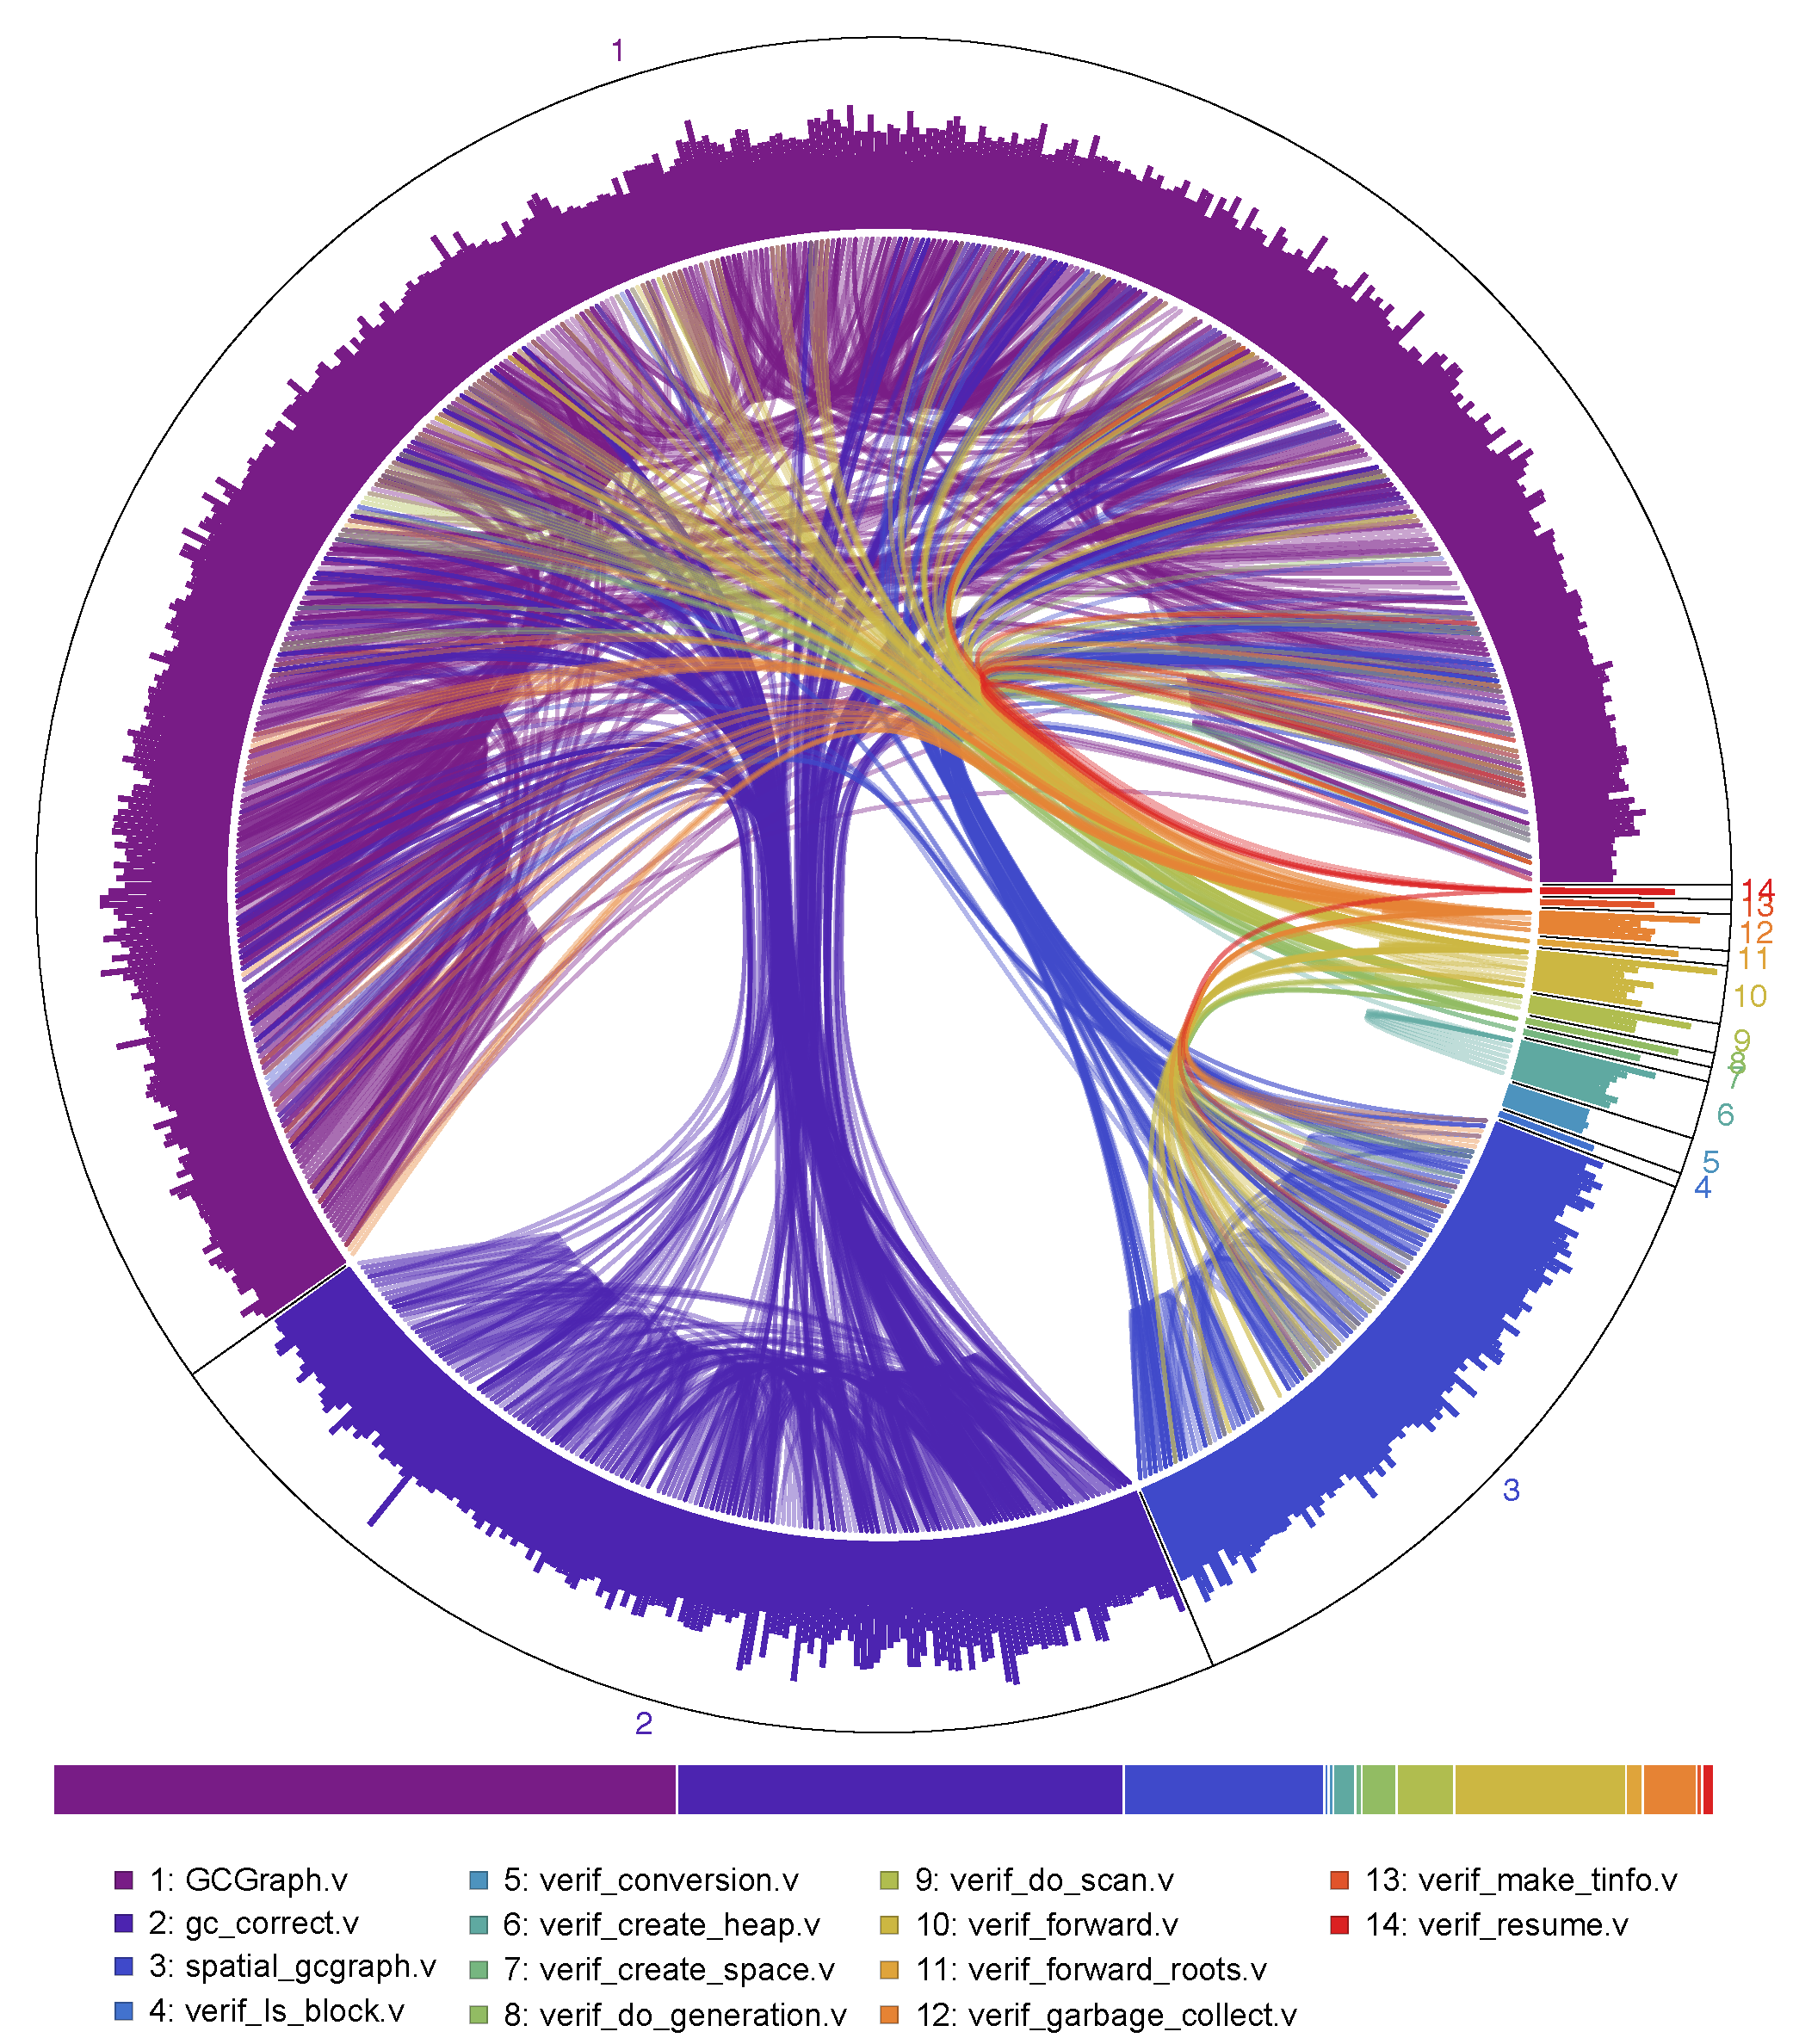
\includegraphics[width=0.95\textwidth]{certigc_theorems}
\caption{\DIFaddFL{Theorems in the verification of the GC}}
\label{fig:connectedness}
\end{figure}

\DIFadd{We worked to make our library modular, thus encouraging 
proof reuse. Figure~\ref{fig:connectedness} gives a sense of this 
engineering effort.
$14$ files were used to verify the garbage collector, and
the bar at the bottom shows their relative lengths.
Each straight line in the perimeter represents a theorem used to verify the GC, 
and the length of a line corresponds to the length of the theorem on a 
logarithmic scale. The $14$ color-coded sectors represent the files in which 
these theorems are housed. Arcs connecting theorems represent dependencies, 
where an arc is colored the same as the theorem's }\emph{\DIFadd{caller}}\DIFadd{.}

\DIFadd{Sector $1$ contains $432$ generic helper theorems used to check that functions
satisfy the inductive spatial relations that we need. These theorems do not depend
on any other GC theorems. Sector $3$ contains $91$ theorems that establish  
spatial correctness (see~\S\ref{sec:spacegraph}). Sectors $4$-$14$ are the actual
proof scripts for individual functions of the C code. Unsurprisingly, they depend
chiefly on Sectors $1$ and~$3$. 
Among these, sector $10$ is notably large, and this makes sense given that it houses 
our workhorse }\li{forward} \DIFadd{function. The C code of }\li{forward} \DIFadd{is~$35$ lines, 
and its verification is~$1309$ lines long: a~$37$-fold blowup.
Sector $2$ contains $155$ theorems that 
prove the final mathematical graph isomorphism (see~\S\ref{sec:mathgraph}).
These theorems depend only on Sector $1$, 
and no other sectors depend on them. This is to be expected, seeing as graph
isomorphism is our final goal. }

\subsection{\texorpdfstring{\DIFadd{Statistics Related to our Development}}{XXX}}
\label{sec:stats}

\DIFaddend \begin{table}[b]
\centering
\DIFaddbeginFL \caption{\DIFaddFL{Statistics for our code base}}
\DIFaddendFL \begin{tabular}{c|c|c|c|c|c}
Component & Section & Files & Size (in lines) & Definitions & Theorems\\\hline
Common Utilities & & 10 & 3,578 & 44 & 289 \\
Math Graph Library & \S\ref{sec:mathgraph} & 20 & 10,585 & 216 & 581 \\
Spatial Graph Library & \S\ref{sec:spacegraph} & 3 & 2,328 & 59 & 110 \\
Integration into VST & \S\ref{sec:localizations},\S\ref{sec:development} & 11 & 2,783 & 17 & 172 \\
\hline
Marking (graph and DAG) & \S\ref{sec:localizations} & 6 & 775 & 9 & 20 \\
Spanning Tree & \S\ref{sec:localizations} & 5 & 2,723 & 17 & 92 \\
Union-Find (heap and array) & \S\ref{sec:orientation} & 18 & 3,193 & 107 & 135 \\
Garbage Collector & \S\ref{sec:certigc} & 16 & 13,858 & 235 & 712 \\
\hline & & & & & \\
[-2.2em] \\
\hline & & & & & \\
[-1em]
Total Development & & 89 & 39,823 & 704 & 2,111 \\
\end{tabular}
\DIFdelbeginFL %DIFDELCMD < \caption{%
{%DIFAUXCMD
\DIFdelFL{Statistics for our code base}}
%DIFAUXCMD
\DIFdelendFL \label{tab:codebase}
\end{table}

All our results in this paper have been machine-checked.
Although the size of a development does not perfectly match \DIFdelbegin \DIFdel{with }\DIFdelend that development's 
importance or \DIFdelbegin \DIFdel{implementation difficulty }\DIFdelend \DIFaddbegin \DIFadd{the difficulty of its implementation}\DIFaddend , 
we present the size nonetheless in Table~\ref{tab:codebase}.
Our proof script is written in a very
dense style.
For comparison, verifying a simple 39-line list-based merge sort in VST takes 600 lines.
At $\approx400$ LOC, the garbage collector is much larger, and is very complicated both
mathematically and spatially, in many places teetering on the edge of what can be defined
in~C. For context, CompCert has 217k LOC, 5,687 definitions, and 6,694 theorems;
VST has 623k LOC, 14,038 definitions, and 21,442 theorems. \DIFaddbegin \DIFadd{It is hard to determine
the time taken for this project on the whole, but the verification of the garbage collector
took us eight months.} \DIFaddend 






\hide{
\paragraph{Size of Coq mathgraph \S\ref{sec:mathgraph}.}
Graph folder has 18 files in total with 10,919 lines in total

\paragraph{Size of Coq spacegraph \S\ref{sec:spacegraph}.}

not including the connection to H/S or VST

include \li{Graph.v} and \li{GraphBi.v} from \li{msl_application} since they do not depend on the underlying VST model?

What is in \li{ramification_lemmas}?  
\paragraph{Integration into Floyd (\S\ref{sec:vst}).}: ?
Size of additions to VST logic model: ?

\paragraph{Modifications to HIP/SLEEK.}
H/S code: approximately 2,500 lines of code across 51 files
Size of extra H/S memory model:
\li{alg_seplog_direct.v}  52 lines
\li{overlapping_direct.v} 442 lines  {\color{magenta}How do we handle alignment?}
\li{precise_direct.v} 111 lines
other files?

\paragraph{Size of VST examples~\S\ref{sec:application}.}

Note: graph, graphbi (in space), graphmark, graphbimark are shared in \li{msl_application}

mark graph  19 + 402 + 161 + 246 = 828
mark dag  19 + 402 + 161 + 210
Note: mark dag shares 19 + 402 + 161 with mark graph

copy   459 + 19 + 161 + 388 = 1,027 (need to add files from \li{msl_applicatin})
dispose   475 + 18 + 544 = 1,037 (need to add files from \li{data_structure})
What do copy or dispose share with mark or with each other?

total: 1,038 (marks) + 2,064 (copy/dispose, assuming no duplication) = 3,102 lines.  12 files, assuming no sharing for copy/dispose (with each other or with mark)

\paragraph{Size of H/S example.}
main file: 54 lines (Figure~\ref{fig:hipmarkgraph}), \li{Module Type} generated by H/S (Figure~\ref{fig:hipcoqfile}) is 30 lines, Coq \li{Module} matching this \li{Module Type} is 358 lines.
total: 2 human-generated files, 429 lines

\paragraph{Size of total development.} ?
}

\section{Related work}
\label{sec:related}
\paragraph{Comparison with~\DIFdelbegin \DIFdel{\mbox{%DIFAUXCMD
\cite{hobor:ramification}}\hspace{0pt}%DIFAUXCMD
}\DIFdelend \DIFaddbegin \DIFadd{\mbox{%DIFAUXCMD
\citet{hobor:ramification}}\hspace{0pt}%DIFAUXCMD
}\DIFaddend .}
Our work builds on the theory of ramification by Hobor and \DIFdelbegin \DIFdel{Villiard}\DIFdelend \DIFaddbegin \DIFadd{Villard}\DIFaddend ,
who verified graph algorithms on pen-and-paper using their \infrulestyle{Ramify} rule:
\begin{equation*}
\inferrule[Ramify]
{\{ L_1 \} ~ c ~ \{ L_2 \} \\
G_1 |- L_1 * (L_2 --* G_2)}
{\{ G_1 \} ~ c ~ \{ G_2 \}} \qquad \mathit{freevars}(L_2 --* G_2) \cap \MV(c) = \emptyset
\end{equation*}
Our \textsc{Localize} rule upgrades \textsc{Ramify} to better handle modified program
variables (note the side condition and recall the discussion in \S\ref{sec:localizations})
and existential quantifiers in postconditions.  Hobor and Villard avoided these challenges
by proposing a unwieldy variant of \infrulestyle{Ramify} called \infrulestyle{RamifyAssign}, which
could reason about the special case of a single assignment $\li{x=}f(\ldots)$, assuming
the verifier can make the local program translation to $\li{x'=}f(\ldots)\li{; x=x'}$,
where \li{x'} is fresh.  This is nontrivial in large existing formal
developments, such as VST, that do not have any way to prove programs equivalent.
Hobor and Villard could not verify unmodified program code, modify program variables
inside nested localization blocks, or handle multiple assignments in a single block as
in lines~\ref{code:markbeforetripleramify}--\ref{code:markaftertripleramify} of
\DIFdelbegin \DIFdel{figure}\DIFdelend \DIFaddbegin \DIFadd{Figure}\DIFaddend ~\ref{fig:markgraph}.  \DIFdelbegin \DIFdel{Hobor and Villard }\DIFdelend \DIFaddbegin \DIFadd{They }\DIFaddend avoided existentials in localized
postconditions by defining all mathematical operations (\emph{e.g.} $\m{mark}$) as
functions rather than as relations; this is fine for pen-and-paper, but painful in
a mechanized setting wherein functions must be proven to terminate.

\DIFdelbegin %DIFDELCMD < \iffalse
%DIFDELCMD < %%%
\DIFdel{Our development is entirely machine-checked~(\S\ref{sec:development}) which revealed some
tricky technique details. }\DIFdelend Hobor and Villard \DIFdelbegin \DIFdel{fell into the trap of defining spatial graphs
recursively~(\S\ref{sec:fixpointfail}); unfortunately other members of the research
community have since followed them in.  We exposed this error and provided a sound,
general, and highly modular graph framework that works smoothly in a mechanized
context~(\S\ref{sec:mathgraph},\S\ref{sec:spacegraph}).
}%DIFDELCMD < \fi
%DIFDELCMD < 

%DIFDELCMD < \iftrue
%DIFDELCMD < %%%
\DIFdel{Hobor and Villard }\DIFdelend treated mathematical graphs as triples $(V,E,L)$ of
vertices, edges, and a vertex labeling function\DIFdelbegin \DIFdel{; }\DIFdelend \DIFaddbegin \DIFadd{, where }\DIFaddend vertices had no more than two
neighbors. Our mathematical graph framework~(\S\ref{sec:mathgraph}) is \DIFdelbegin \DIFdel{very
modular and general and }\DIFdelend \DIFaddbegin \DIFadd{more
modular and versatile, and ships with hundreds of reusable definitions and theorems. Further, our library }\DIFaddend has been tuned to work smoothly in a mechanized context.


Hobor and Villard erroneously defined spatial graphs
recursively\DIFdelbegin \DIFdel{~(\S\ref{sec:fixpointfail}); unfortunately }\DIFdelend \DIFaddbegin \DIFadd{. Unfortunately, }\DIFaddend other members of the research
community \DIFdelbegin \DIFdel{have since followed them in, }\DIFdelend \DIFaddbegin \DIFadd{(}\DIFaddend \emph{e.g.}~\DIFdelbegin \DIFdel{\mbox{%DIFAUXCMD
\cite{raadvg15}}\hspace{0pt}%DIFAUXCMD
.  We exposed this
errorand provided }\DIFdelend \DIFaddbegin \DIFadd{\mbox{%DIFAUXCMD
\citet{raadvg15}}\hspace{0pt}%DIFAUXCMD
) followed their lead.  We expose this
error~(\S\ref{sec:fixpointfail}) and provide }\DIFaddend a sound and \DIFdelbegin \DIFdel{quite }\DIFdelend \DIFaddbegin \DIFadd{rather }\DIFaddend general definition for
\p{graph} \DIFdelbegin \DIFdel{~(\S\ref{sec:goodgraph}) }\DIFdelend that recovers fold/unfold reasoning\DIFdelbegin \DIFdel{.  We developed }\DIFdelend \DIFaddbegin \DIFadd{~(\S\ref{sec:goodgraph}).  We develop }\DIFaddend a
much more general and more modular set of related lemmas and \DIFdelbegin \DIFdel{connect }\DIFdelend \DIFaddbegin \DIFadd{connected }\DIFaddend our spatial
reasoning to the verification framework of CompCert/VST~(\S\ref{sec:vst})\DIFdelbegin \DIFdel{, and
our }\DIFdelend \DIFaddbegin \DIFadd{.
Our }\DIFaddend development is entirely
machine-checked~(\S\ref{sec:development}) whereas they used only pen and paper.

\DIFdelbegin %DIFDELCMD < \fi
%DIFDELCMD < %%%
\DIFdelend \DIFaddbegin \paragraph{\DIFadd{Other Pen-and-Paper Verification of Graph Algorithms and/or $**$.}}
\DIFaddend 

\DIFdelbegin \paragraph{\DIFdel{Other verification of graph algorithms and/or $**$.}}
%DIFAUXCMD
\addtocounter{paragraph}{-1}%DIFAUXCMD
\DIFdel{\mbox{%DIFAUXCMD
\cite{hongseok:phd}}\hspace{0pt}%DIFAUXCMD
's verification of }\DIFdelend \DIFaddbegin \DIFadd{\mbox{%DIFAUXCMD
\citet{hongseok:phd} }\hspace{0pt}%DIFAUXCMD
verified }\DIFaddend the Schorr-Waite algorithm\DIFdelbegin \DIFdel{is }\DIFdelend \DIFaddbegin \DIFadd{, and this 
is widely considered }\DIFaddend a landmark in the early separation logic literature. 
\DIFdelbegin \DIFdel{\mbox{%DIFAUXCMD
\cite{neelthesis}}\hspace{0pt}%DIFAUXCMD
~provided the first separation
logic proof of union-find.  \mbox{%DIFAUXCMD
\cite{bornat:aliasing04}}\hspace{0pt}%DIFAUXCMD
~}\DIFdelend \DIFaddbegin \DIFadd{\mbox{%DIFAUXCMD
\citet{bornat:aliasing04}}\hspace{0pt}%DIFAUXCMD
~}\DIFaddend gave an early attempt to reason about graph algorithms 
in separation logic in a more general way. 
\DIFaddbegin \DIFadd{\mbox{%DIFAUXCMD
\citet{neelthesis}}\hspace{0pt}%DIFAUXCMD
~provided the first separation logic proof of union-find.
}\DIFaddend 

\DIFdelbegin \DIFdel{\mbox{%DIFAUXCMD
\cite{rey-slnotes}}\hspace{0pt}%DIFAUXCMD
}\DIFdelend \DIFaddbegin \DIFadd{\mbox{%DIFAUXCMD
\citet{rey-slnotes}}\hspace{0pt}%DIFAUXCMD
}\DIFaddend ~was the first to document the overlapping 
conjunction \DIFdelbegin \DIFdel{~}\DIFdelend $**$, albeit without any strategy to reason about it using Hoare rules. 
\DIFdelbegin \DIFdel{\mbox{%DIFAUXCMD
\cite{gardnerms12}}\hspace{0pt}%DIFAUXCMD
}\DIFdelend \DIFaddbegin \DIFadd{\mbox{%DIFAUXCMD
\citet{gardnerms12}}\hspace{0pt}%DIFAUXCMD
}\DIFaddend ~were the first to reason about a program using $**$ in 
Javascript. 
\DIFdelbegin \DIFdel{\mbox{%DIFAUXCMD
\cite{raadvg15}}\hspace{0pt}%DIFAUXCMD
}\DIFdelend \DIFaddbegin \DIFadd{\mbox{%DIFAUXCMD
\citet{raadvg15}}\hspace{0pt}%DIFAUXCMD
}\DIFaddend ~used $**$ \DIFaddbegin \DIFadd{within their CoLoSL program logic }\DIFaddend to reason about 
a concurrent spanning algorithm using a kind of ``concurrent localization''.
\DIFdelbegin \DIFdel{\mbox{%DIFAUXCMD
\cite{ilya-graphs} }\hspace{0pt}%DIFAUXCMD
also verified }\DIFdelend \DIFaddbegin 



\paragraph{\DIFadd{Machine-Checked Verification of Graph Algorithms.}}
\DIFadd{A decade after Yang verified Schorr-Waite on paper, \mbox{%DIFAUXCMD
\citet{leino10} }\hspace{0pt}%DIFAUXCMD
automated 
its verification in Dafny. 
\mbox{%DIFAUXCMD
\citet{ilya-graphs}}\hspace{0pt}%DIFAUXCMD
~verified }\DIFaddend a concurrent spanning tree algorithm, and 
moreover developed mechanized Coq proofs. \DIFaddbegin \DIFadd{Their algorithm was written in FCSL, 
a monadic DSL that combines effectful operations with pure Coq expressions; 
FSCL cannot be executed. 
\mbox{%DIFAUXCMD
\citet{chen18}}\hspace{0pt}%DIFAUXCMD
~compared how three provers (Coq, Isabelle, and Why3) can 
verify Tarjan’s strongly-connected component algorithm written in the native 
language of each of the tools. Because these are written in the native languages 
of a proof assistant, they avoid “real-world” language concerns such as 
memory models and overflow.
}\DIFaddend 

\DIFdelbegin \DIFdel{A decade after Yang verified Schorr-Waite on paper, 
\mbox{%DIFAUXCMD
\cite{leino10}}\hspace{0pt}%DIFAUXCMD
~automated
its verification.
}\DIFdelend \DIFaddbegin \DIFadd{\mbox{%DIFAUXCMD
\citet{lamneu15}}\hspace{0pt}%DIFAUXCMD
~extended the Isabelle Refinement Framework to verify a range of 
DFS algorithms via stepwise refinement.
Their framework allows the reuse of previously-proved DFS 
invariants by establishing an inductive
``most specific invariant'' and deriving other inductive invariants from it.
\mbox{%DIFAUXCMD
\citet{lamsef19}}\hspace{0pt}%DIFAUXCMD
~extended this further and presented verifications of 
the correctness and time complexity of the Edmonds-Karp and push-relabel
algorithms. Lammich et al. produced very readable proofs of classic 
textbook algorithms by using the Isar language atop their Isabelle proofs.
They used Isabelle's code generator to export efficient executable code, 
but with the caveat that the code comes with a guarantee of only 
partial correctness semantics.
}\DIFaddend 

\DIFdelbegin %DIFDELCMD < \vspace{-1ex}
%DIFDELCMD < %%%
\DIFdelend \DIFaddbegin \DIFadd{\mbox{%DIFAUXCMD
\citet{char11}}\hspace{0pt}%DIFAUXCMD
~used his CFML tool to Coq-verify an OCaml implementation of 
Dijkstra. 
\mbox{%DIFAUXCMD
\citet{gueneauetal19}}\hspace{0pt}%DIFAUXCMD
~extended CFML and verified the correctness 
and time complexity of a modified version of the BFGT cycle-detection algorithm.
The graph algorithms verified in CFML tend to be ``graph theory'' in flavour, 
whereas the algorithms we have verified tend to have more of a
``systems'' flavor. This difference is partially explained by the fact that 
code written in ML can take advantage of its high-level design, whereas
code written in C is often interested in handling grungy systems tasks. For 
example, references in ML cannot be null and do not support pointer arithmetic; 
of course both are possible---and lead to nontrivial complications---in 
C. Accordingly, the CFML proofs benefit from ML’s cleaner computational model. 
Our verifications are in C so we must contend with C’s memory model, pointer 
arithmetic, significant scope for undefined behavior, and so forth.
}

\DIFadd{\mbox{%DIFAUXCMD
\citet{charpott15, charpott19}}\hspace{0pt}%DIFAUXCMD
~used CFML to verify the correctness and 
time complexity of union-find. Their work is an interesting counterpoint to 
ours because, while it maintains an abstraction between the client and the 
internal mathematical/spatial facts that the client need not know, it does 
not maintain a separation between the mathematical and spatial 
facts themselves, as we do in~\S\ref{sec:mathgraph} and ~\S\ref{sec:spacegraph}.
This separation is worthwhile: our modular method let us verify an alternate 
version of union-find that uses an array of vertices rather than individually 
heap-allocated nodes. This 
secondary verification then used }\emph{\DIFadd{exactly the same}} \DIFadd{mathematical proof of 
functional correctness despite the radically different layout of spatial 
memory.
Our work does not verify the time complexity of union-find. When 
we attempted to prove the necessary amortisation bounds we ran into an 
overflow issue: it was impossible to prove that the rank would not exceed 
}\li{max\_int} \DIFadd{because the CompCert memory model does not place a bound on the 
total number of allocations. Informally, this overflow is impossible in 
practice because no computer has $2^{2^{\tiny 64}}$ bytes of memory, which would 
be required for this overflow to occur, but Coq remains unconvinced. 
Chargu}{\DIFadd{\'{e}}}\DIFadd{raud and Pottier acknowledged and sidestepped this issue by 
representing rank using the Coq type }\li{Z}\DIFadd{, which was not an option for us 
given the end-to-end nature of the VST+CompCert toolchain.
}

\DIFaddend \paragraph{Verification \DIFdelbegin \DIFdel{tools}\DIFdelend \DIFaddbegin \DIFadd{Tools in Coq}\DIFaddend .}
Our work interacts with the Floyd \DIFdelbegin \DIFdel{~\mbox{%DIFAUXCMD
\cite{appel:programlogics} }\hspace{0pt}%DIFAUXCMD
verification
tool. 
}\DIFdelend \DIFaddbegin \DIFadd{verification module within the Verified 
Software Toolchain (VST)~\mbox{%DIFAUXCMD
\cite{appel:programlogics}}\hspace{0pt}%DIFAUXCMD
. The Floyd module uses 
tactics to enable the separation-logic verification of CompCert C programs. 
VST connects to the CompCert certified C compiler~\mbox{%DIFAUXCMD
\cite{leroy:compcert}}\hspace{0pt}%DIFAUXCMD
, and 
thus has no gaps or admits between the verified source code and the eventual
assembly code~\mbox{%DIFAUXCMD
\cite{appelvst}}\hspace{0pt}%DIFAUXCMD
.
}

\DIFaddend Charge! likewise uses Coq tactics to work with a shallow embedding of higher 
order separation logic, but focuses on OO programs written in 
Java/C\#~\DIFaddbegin \DIFadd{~}\DIFaddend \cite{bengtson:charge}. Iris Proof Mode provides a similar framework 
for higher-order concurrent reasoning \DIFaddbegin \DIFadd{in Coq}\DIFaddend ~\cite{krebbers:iris}.
\DIFdelbegin \DIFdel{A  }\DIFdelend \DIFaddbegin 

\DIFadd{CFML enables the verification of OCaml programs by reasoning about their
``characteristic formulae'' in separation logic using Coq~\mbox{%DIFAUXCMD
\cite{char10, char11}}\hspace{0pt}%DIFAUXCMD
. 
CFML has been used to verify a range of functional and imperative programs,
including some graph-related algorithms as discussed 
above. \mbox{%DIFAUXCMD
\citet{charpott15, charpott19}}\hspace{0pt}%DIFAUXCMD
~extended CFML to reason about time 
credits. The work of \mbox{%DIFAUXCMD
\citet{gueneau17}}\hspace{0pt}%DIFAUXCMD
~indicates that CFML is exploring a connection 
with the certified CakeML compiler~\mbox{%DIFAUXCMD
\cite{cakeml}}\hspace{0pt}%DIFAUXCMD
.
}

\DIFadd{While the tools above require substantial human guidance, 
Bedrock~\mbox{%DIFAUXCMD
\cite{chlipala:bedrock} }\hspace{0pt}%DIFAUXCMD
is a }\DIFaddend more automated approach to \DIFaddbegin \DIFadd{the }\DIFaddend verification of 
low level programs using \DIFdelbegin \DIFdel{Coq is the Bedrock framework \mbox{%DIFAUXCMD
\cite{chlipala:bedrock}}\hspace{0pt}%DIFAUXCMD
.
}\DIFdelend \DIFaddbegin \DIFadd{separation logic in Coq. 
Bedrock leverages the fact that phrasing function 
specifications in a }\emph{\DIFadd{computational}} \DIFadd{style 
(in this case, inspired by functional programming) 
leads to separation logic proof obligations that are quite automatable.
It simplifies these obligations into pure mathematics using a 
custom workhorse tactic, and then discharges those 
obligations using standard Coq automation.
}\DIFaddend 

\DIFdelbegin \DIFdel{Many automated }\DIFdelend \DIFaddbegin \paragraph{\DIFadd{Other Verification Tools.}} 

\DIFadd{Many more-automated }\DIFaddend verification tools also use separation logic in a forward
reasoning style\DIFdelbegin \DIFdel{as does HIP/SLEEK, including }\DIFdelend \DIFaddbegin \DIFadd{. }\DIFaddend Smallfoot~\cite{berdine:smallfoot}, jStar~\DIFdelbegin \DIFdel{\mbox{%DIFAUXCMD
\cite{distefanop08}}\hspace{0pt}%DIFAUXCMD
, and Verifast~\mbox{%DIFAUXCMD
\cite{jacobs:verifast}}\hspace{0pt}%DIFAUXCMD
.  One of }\DIFdelend \DIFaddbegin \DIFadd{~\mbox{%DIFAUXCMD
\cite{distefanop08}}\hspace{0pt}%DIFAUXCMD
, 
}\DIFaddend HIP/SLEEK\DIFdelbegin \DIFdel{'s
distinguishing features is good support for user-defined inductive predicates rather
than a library of pre-defined predicates for lists, trees etc.
}%DIFDELCMD < 

%DIFDELCMD < %%%
\DIFdel{Dafny~\mbox{%DIFAUXCMD
\cite{leino10} }\hspace{0pt}%DIFAUXCMD
and }\DIFdelend \DIFaddbegin \DIFadd{~\mbox{%DIFAUXCMD
\cite{chin:hipsleek}}\hspace{0pt}%DIFAUXCMD
, and Verifast~\mbox{%DIFAUXCMD
\cite{jacobs:verifast} }\hspace{0pt}%DIFAUXCMD
are landmarks
at various points on the expressibility-automatability spectrum. 
}\DIFaddend KeY~\cite{beckert:2007} \DIFdelbegin \DIFdel{are verifiers }\DIFdelend \DIFaddbegin \DIFadd{and Dafny~\mbox{%DIFAUXCMD
\cite{leino10} }\hspace{0pt}%DIFAUXCMD
are verifiers that are }\DIFaddend not 
based on separation logic\DIFdelbegin \DIFdel{; }\DIFdelend \DIFaddbegin \DIFadd{. }\DIFaddend KeY uses an interactive verifier while Dafny pursues
 automation with Z3~\cite{moura2008}.

\DIFdelbegin %DIFDELCMD < \vspace{-1ex}
%DIFDELCMD < %%%
\DIFdelend \paragraph{Mechanized \DIFdelbegin \DIFdel{mathematical graph theory}\DIFdelend \DIFaddbegin \DIFadd{Mathematical Graph Theory}\DIFaddend .}
There is a long history, going back at least \DIFdelbegin \DIFdel{25 }\DIFdelend \DIFaddbegin \DIFadd{28 }\DIFaddend years, of mechanized 
reasoning about mathematical graphs~\cite{wong1991}. 
The most famous mechanically verified \DIFdelbegin \DIFdel{``graph theorem''
}\DIFdelend \DIFaddbegin \DIFadd{“graph theorem” }\DIFaddend is the Four Color 
Theorem~\cite{gonthier2005computer}; however the development actually uses
hypermaps instead of graphs. \DIFdelbegin \DIFdel{Noschinski }\DIFdelend \DIFaddbegin \DIFadd{In general most “mathematical graph” frameworks in 
the literature~\mbox{%DIFAUXCMD
\cite{wong1991, chou1994, yamamoto1995formalization, rwpgt1998, yamamoto1998formalization, tamai2000formal, duprat2001coq, ridge2005graphs, nipkow2016, dijkstra_shortest_path-afp} }\hspace{0pt}%DIFAUXCMD
were not used to verify real 
code, for which they seem unsuitable. Verifying real code requires delicate concepts such as removing a subgraph, null nodes, and parallel edges, and one of our contributions is that our framework is general enough to support such verification. 
\mbox{%DIFAUXCMD
\citet{noschinski2015}}\hspace{0pt}%DIFAUXCMD
~}\DIFaddend built a graph library in Isabelle/HOL whose formalization 
is the closest to ours\DIFdelbegin \DIFdel{~\mbox{%DIFAUXCMD
\cite{noschinski2015}}\hspace{0pt}%DIFAUXCMD
}\DIFdelend , 
\emph{e.g.} supporting graphs with labeled and parallel arcs. 
\DIFdelbegin \DIFdel{\mbox{%DIFAUXCMD
\cite{noschinski2015formalizing,dubois2015graphes}}\hspace{0pt}%DIFAUXCMD
~used }\DIFdelend \DIFaddbegin \DIFadd{Beyond being in Coq, our setup supports at least three features beyond 
Noschinski’s: reasoning about incomplete graphs (as discussed 
in~\S\ref{sec:mathinfra} using figure~\ref{fig:pregraph}), labeling the graph 
as a whole (used, for example, in the garbage collector to store 
metainformation about the number and location of the generations), and our 
modular typeclass-supported “graphs with properties” setup in General Graph 
(as described in~\S\ref{subsec:graphplugins}). 
\mbox{%DIFAUXCMD
\citet{dubois2015graphes} }\hspace{0pt}%DIFAUXCMD
and \mbox{%DIFAUXCMD
\citet{noschinski2015formalizing}}\hspace{0pt}%DIFAUXCMD
~used }\DIFaddend proof assistants to 
design verifiable checkers for solutions to graph problems. 
\DIFdelbegin \DIFdel{\mbox{%DIFAUXCMD
\cite{yamamoto1995formalization,bauer20025}}\hspace{0pt}%DIFAUXCMD
~use }\DIFdelend \DIFaddbegin \DIFadd{\mbox{%DIFAUXCMD
\citet{bauer20025} }\hspace{0pt}%DIFAUXCMD
and \mbox{%DIFAUXCMD
\citet{yamamoto1995formalization}}\hspace{0pt}%DIFAUXCMD
~used }\DIFaddend an inductive encoding of graphs to formalize planar graph theory.


\DIFdelbegin \DIFdel{\mbox{%DIFAUXCMD
\cite{gueneauetal}}\hspace{0pt}%DIFAUXCMD
~formalised ``time credits'' in Separation Logic and big-$O$ notation in
Coq and then verified both the correctness
and the time complexity of the union-find data structure.
}%DIFDELCMD < 

%DIFDELCMD < %%%
\DIFdelend \paragraph{Verification of \DIFdelbegin \DIFdel{garbage collection algorithms}\DIFdelend \DIFaddbegin \DIFadd{Garbage Collection Algorithms}\DIFaddend .}
Schism \cite{gcexample4,gcexample4a} is a certified concurrent
collector built in a Java VM that services multi-core architectures with weak memory consistency.
\DIFdelbegin \DIFdel{McCreight }\emph{\DIFdel{et al.}} %DIFAUXCMD
\DIFdel{\mbox{%DIFAUXCMD
\cite{gcexample5, gcexample3} }\hspace{0pt}%DIFAUXCMD
introduce }\DIFdelend \DIFaddbegin \DIFadd{\mbox{%DIFAUXCMD
\citet{gcexample5, gcexample3} }\hspace{0pt}%DIFAUXCMD
introduced }\DIFaddend GCminor, which is
a certified translation step added to CompCert's translation from Clight to assembly.
GCminor makes explicit the specific invariants that the garbage collector
relies upon, thus minimising errors due to the violation of invariants
between the garbage collector and the mutator.
\DIFdelbegin \DIFdel{Hawblitzel and Petrank \mbox{%DIFAUXCMD
\cite{gcexample2} }\hspace{0pt}%DIFAUXCMD
annotate }\DIFdelend \DIFaddbegin \DIFadd{\mbox{%DIFAUXCMD
\citet{gcexample2} }\hspace{0pt}%DIFAUXCMD
annotated }\DIFaddend x86 code
for two GCs by hand, and then \DIFdelbegin \DIFdel{use }\DIFdelend \DIFaddbegin \DIFadd{used }\DIFaddend Boogie and the Z3 automated theorem prover
to verify their correctness automatically.

The closest piece of work to our certified GC is probably the excellent certified GC
for the Cake ML project~\cite{cakemlgc}, since both integrate a certified GC into 
a certified compiler for a functional language.  Their GC is written closer to assembly 
than C, which is both a positive---in that they avoid undefined behaviors---and a negative, 
in that their GC is harder to understand and upgrade and cannot take advantage of the
mature CompCert compiler.  Their GC lacks some of our optimisations (\emph{e.g.} they have 
only three generations), but on the other hand handles mutation in the GC heap.  The largest 
difference, however, is that we present an integrated graph framework suitable for reasoning 
about many graph algorithms, of which our GC is merely the flagship.  In contrast, they focus 
much more narrowly on the problem of certified GCs.

\section{Future work and conclusion}
\label{sec:future}
\label{sec:conclusion}
In the future we plan to improve the pure reasoning of graphs and
similar data structures, \DIFdelbegin \DIFdel{in particular to add }\DIFdelend \DIFaddbegin \DIFadd{with a particular focus on }\DIFaddend automation.  We have
also begun to investigate integrating our techniques into the 
HIP/SLEEK toolchain~\cite{chin:hipsleek}, which\DIFaddbegin \DIFadd{, }\DIFaddend as compared to VST\DIFaddbegin \DIFadd{, }
\DIFaddend provides more automation at the cost of lower expressivity.  We
are also interested in investigating better ways to handle the
kinds of undefined behavior upon which real~C systems code sometimes
relies.

\hide{\color{magenta}We are in the process of verifying a garbage
collector for the ``CertiCoq'' project, which is building
a certified compiler from Gallina to Clight. We would like to investigate
using our externally verified lemmas in HIP/SLEEK to verify code such as fast
exponentiation and more graph algorithms. We also would like to make
the interface between Coq and H/S simpler and cleaner.
One final direction we would like to investigate is using our new
connection to Coq to have H/S output certificates as it
verifies programs so that the system becomes more trustworthy.}

Our main contributions were as follows.  We developed a mathematical
graph library that was powerful enough to reason about graph-manipulating
algorithms written in real~C code.  We connected these mathematical graphs
to spatial graphs in the heap via separation logic.  We developed 
localization blocks to smoothly reason about a local action's effect on
a global context in a mechanized context, including a robust treatment
of modified program variables and existential quantifiers in postconditions.
We demonstrated our techniques on several nontrivial examples, including union-find
and spanning tree.  Our flagship example \DIFdelbegin \DIFdel{is }\DIFdelend \DIFaddbegin \DIFadd{was }\DIFaddend the verification of the garbage collector 
for the CertiCoq project, during which we found two places in which the~C semantics
is too weak to define an OCaml-style GC.  We integrated our techniques into the
VST toolset. 

\begin{acks}
\DIFaddbegin \DIFadd{
We thank Asankhaya Sharma for his help with a previous version of this paper,
Neel Krishnaswami for his helpful suggestions and encouragements, and 
Xavier Leroy and Robbert Krebbers for fruitful discussions. 
We also thank the CertiCoq team (esp. Andrew~W.~Appel, Olivier~Savary~Belanger, and 
Zoe~Paraskevopoulou) for their overall support and for hosting 
Shengyi Wang for a summer. This work was funded in part by the
\grantsponsor{}{Yale-NUS College}{} grant~\mbox{\grantnum{}{R-607-265-322-121}} and the \grantsponsor{}{National Science \linebreak Foundation}{} grant~\grantnum{}{CCF-1521602}.
Any opinions, findings, and conclusions or recommendations expressed in 
this material are those of the authors and do not necessarily reflect the 
views of Yale-NUS College or the National Science Foundation.}\DIFaddend
\end{acks}

\hide{ 
\begin{acks}
\DIFdelbegin \DIFdel{This material is based upon work supported by the
  }%DIFDELCMD < \grantsponsor{GS100000001}{National Science
%DIFDELCMD <     Foundation}{http://dx.doi.org/10.13039/100000001} %%%
\DIFdel{under Grant
  No.~}%DIFDELCMD < \grantnum{GS100000001}{nnnnnnn} %%%
\DIFdel{and Grant
  No.~}%DIFDELCMD < \grantnum{GS100000001}{mmmmmmm}%%%
\DIFdel{.  Any opinions, findings, and
  conclusions or recommendations expressed in this material are those
  of the author and do not necessarily reflect the views of the
  National Science Foundation.
}\DIFdelend \DIFaddbegin \DIFadd{We thank Asankhaya Sharma for his help with a previous version of this paper,
Neel Krishnaswami for his helpful suggestions and encouragements, and 
Xavier Leroy and Robbert Krebbers for fruitful discussions. 
We also thank the CertiCoq team (esp. Andrew~W.~Appel, Olivier~Savary~Belanger, and 
Zoe~Paraskevopoulou) for their overall support and for hosting 
Shengyi Wang for a summer. This work was funded in part by the
}\grantsponsor{}{Yale-NUS College}{} \DIFadd{grant~\mbox{\grantnum{}{R-607-265-322-121}} and the }\grantsponsor{}{National Science Foundation}{} \DIFadd{grant~}\grantnum{}{CCF-1521602}\DIFadd{.
Any opinions, findings, and conclusions or recommendations expressed in 
this material are those of the authors and do not necessarily reflect the 
views of Yale-NUS College or the National Science Foundation.}
\hide{

This material is based upon work supported by the
  \grantsponsor{GS100000001}{National Science
    Foundation}{http://dx.doi.org/10.13039/100000001} under Grant
  No.~\grantnum{GS100000001}{nnnnnnn} and Grant
  No.~\grantnum{GS100000001}{mmmmmmm}.  Any opinions, findings, and
  conclusions or recommendations expressed in this material are those
  of the author and do not necessarily reflect the views of the
  National Science Foundation.}
\DIFaddend \end{acks} }

\DIFdelbegin %DIFDELCMD < \bibliography{autoquack.bib}
%DIFDELCMD < 

%DIFDELCMD < \appendix
%DIFDELCMD < 

%DIFDELCMD < %%%
\section{\texorpdfstring{\DIFdel{Spanning and Copying}}{XXX}}
%DIFAUXCMD
\addtocounter{section}{-1}%DIFAUXCMD
%DIFDELCMD < \label{apx:spanning}
%DIFDELCMD < 

%DIFDELCMD < \begin{figure}[t]
%DIFDELCMD <
\begin{lstlisting}
struct Node {
    int m;
    struct Node * l;
    struct Node * r; };
// We use $R$ to represent $\p{reachable}(\gamma,\tx x)$
void spanning(struct Node * x) { 
// $\{\p{graph}(\tx{x},\gamma)/|\gamma(\tx{x}).1=0\}$ 
    struct Node * l, * r; int root_mark;
// $\{\p{graph}(\tx x,\gamma) /| \exists l,r.~ \gamma(\tx{x}) = (0,l,r)\}$
// $\{\p{graph}(\tx x,\gamma) /| \gamma(\tx{x}) = (0,l,r)\}$
// $\{\p{vertices\_at}(\p{reachable}(\gamma,\tx x), \gamma) /| \gamma(\tx{x}) = (0,l,r)\}$
// $\{\p{vertices\_at}(R, \gamma) /| \gamma(\tx{x}) = (0,l,r)\}$
// $\searrow \{\tx x|-> 0,l,r /| \gamma(\tx{x}) = (0,l,r)\}$
    l = x -> l; r = x -> r; x -> m = 1;
// $\swarrow \{\tx x|-> 1,\tx{l},\tx{r} /| \gamma(\tx{x}) = (0,\tx{l},\tx{r}) /| \exists \gamma_1.~ \m{mark1}(\gamma, \tx{x}, \gamma_1)\}$
// $\{\exists \gamma_1.~\p{vertices\_at}(R, \gamma_1) /| \gamma(\tx{x}) = (0,\tx{l},\tx{r}) /| \m{mark1}(\gamma, \tx{x}, \gamma_1)\}$
// $\{\p{vertices\_at}(R, \gamma_1) /| \gamma(\tx{x}) = (0,\tx{l},\tx{r}) /| \m{mark1}(\gamma, \tx{x}, \gamma_1)\}$
    if (l) {
        root_mark = l -> m;
        if (root_mark == 0) {
            spanning(l);
        } else { x -> l = 0; } }
// $\left\{\!\!\!\begin{array}{l@{}}\exists\gamma_2. ~\p{vertices\_at}(R,\gamma_2)/| \gamma(\tx{x}) = (0,\tx{l},\tx{r})  /| \null \\ \m{mark1}(\gamma, \tx{x}, \gamma_1) /| \m{e\_span}(\gamma_1,\tx{x}.\text{L},\gamma_2)\end{array}\right\}$
// $\left\{\!\!\!\begin{array}{l@{}}\p{vertices\_at}(R,\gamma_2)/| \gamma(\tx{x}) = (0,\tx{l},\tx{r})  /| \null \\ \m{mark1}(\gamma, \tx{x}, \gamma_1) /|  \m{e\_span}(\gamma_1,\tx{x}.\text{L},\gamma_2)\end{array}\right\}$
    if (r) {
        root_mark = r -> m;
        if (root_mark == 0) {
           spanning(r);
        } else { x -> r = 0; } }
// $\left\{\!\!\!\begin{array}{l@{}}\exists\gamma_3.~\p{vertices\_at}(R,\gamma_3)/| \gamma(\tx{x}) = (0,\tx{l},\tx{r})  /| \null \\ \m{mark1}(\gamma, \tx{x}, \gamma_1) /| \m{e\_span}(\gamma_1,\tx{x}.\text{L},\gamma_2) /| \m{e\_span}(\gamma_2,\tx{x}.\text{R},\gamma_3)\end{array}\right\}$
} // $\{\exists \gamma_3.~\p{vertex\_at}(\p{reachable}(\gamma, \tx{x}), \gamma_3)/|\m{span}(\gamma,\tx{x},\gamma_3)\}$
  \end{lstlisting}
%DIFDELCMD <   \small
%DIFDELCMD < %%%
\begin{eqnarray*}
  \DIFdelFL{\p{vertices\_at}(\p{reachable}(\gamma_1, \tx x), \gamma_2)\defeq \underset{v\in\p{reachable}(\gamma_1, \tx x)}{\bigstar}v \mapsto \gamma_2(v)}\\
  \DIFdelFL{\begin{split}
  \m{span}(\gamma_1, \tx x, \gamma_2)\defeq &\m{mark}(\gamma_1,\tx x, \gamma_2) /| \gamma_1\!\uparrow(\lambda v. x\mathrel{{\stackrel{\gamma_1~}{\leadsto^{\star}_{0}}}} v) \text{ is a tree} /| \null\\
  & \gamma_1\!\uparrow\!(\lambda v.\neg x\mathrel{{\stackrel{\gamma_1~}{\leadsto^{\star}_{0}}}} v) = \gamma_2\!\uparrow\!(\lambda v.\neg x\mathrel{{\stackrel{\gamma_1~}{\leadsto^{\star}_{0}}}} v) /| \null\\
  & (\forall v.~x\mathrel{{\stackrel{\gamma_1~}{\leadsto^{\star}_{0}}}} v => \gamma_2\models x \leadsto v) /| \null\\
  & (\forall a,b.~x\mathrel{{\stackrel{\gamma_1~}{\leadsto^{\star}_{0}}}} a => \neg x\mathrel{{\stackrel{\gamma_1~}{\leadsto^{\star}_{0}}}} b => \neg \gamma_2\models a \leadsto b)\\
  \end{split}}\\
  \DIFdelFL{\m{e\_span}(\gamma_1, e, \gamma_2)\defeq
  \begin{cases}
    \gamma_1 - e = \gamma_2  & t(\gamma_1,e)=1\\
    \m{span}(\gamma_1, t(\gamma_1,e), \gamma_2) & t(\gamma_1,e)=0\\
  \end{cases}
}\end{eqnarray*}
%DIFAUXCMD
%DIFDELCMD < \caption{%
{%DIFAUXCMD
\DIFdelFL{Clight code and proof sketch for bigraph spanning tree.}}
%DIFAUXCMD
%DIFDELCMD < \label{fig:spanning}
%DIFDELCMD < 

%DIFDELCMD < \end{figure}
%DIFDELCMD <  

%DIFDELCMD < %%%
\DIFdel{In Figure~\ref{fig:spanning} we show a simplified proof script for the spanning tree algorithm.  Unlike graph marking, the spanning tree algorithm changes the
structure of the graph, leading to a more complicated specification,
in both the pure part and the spatial part. Observe that the $\m{span}$ relation is
rather long; the $\m{e\_span}$ handles the case of either calling spanning tree or deleting an edge.
}%DIFDELCMD < 

%DIFDELCMD < %%%
\DIFdel{We put the proof sketch of the graph copying algorithm in
Figure~\ref{fig:copy-part1} and Figure~\ref{fig:copy-part2}. Just like
other parts of the paper,
both algorithms have been machine verified.
}%DIFDELCMD < 

%DIFDELCMD < \begin{figure}
%DIFDELCMD <
\begin{lstlisting}
struct Node {
    int m;
    struct Node * l;
    struct Node * r; };
// We use $x \xleftrightarrow{\gamma} x'$ to represent $x = x' = 0 \vee \gamma(x) = (x', \_, \_)$
struct Node * copy(struct Node * x) { 
    struct Node * l, * r, * x0, * l0, * r0;
// $\{\p{graph}(\tx{x},\gamma)\}$
      if (x == 0)
        return 0;
// $\{\p{graph}(\tx{x},\gamma)/| x\neq 0\}$
// $\{\p{graph}(\tx x,\gamma) /| \exists x_0,l,r.~ \gamma(\tx{x}) = (x_0,l,r)\}$
// $\{\p{graph}(\tx x,\gamma) /| \gamma(\tx{x}) = (x_0,l,r)\}$
// $\searrow \{\tx x|-> x_0,l,r /| \gamma(\tx{x}) = (x_0,l,r)\}$
      x0 = x -> m;
// $\swarrow \{\tx x|-> x_0,l,r /| \gamma(\tx{x}) = (x_0,l,r) /| \tx{x0} = x_0\}$
// $\{\p{graph}(\tx x,\gamma) /| \gamma(\tx{x}) = (\tx{x0},l,r)\}$
      if (x0 != 0)
        return x0;
// $\{\p{graph}(\tx x,\gamma) /| \gamma(\tx{x}) = (0,l,r) \}$
      x0 = (struct Node *) mallocN (sizeof (struct Node));
// $\{\p{graph}(\tx x,\gamma) * \tx{x0} |-> \_, \_, \_ /| \gamma(\tx{x}) = (0,l,r) \}$
// $\searrow \{\tx x|-> 0,l,r * \tx{x0} |-> \_, \_, \_ /| \gamma(\tx{x}) = (0,l,r)\}$
      l = x -> l; r = x -> r; x -> m = x0; x0 -> m = 0;
// $\swarrow \left\{\!\!\!\begin{array}{l@{}} \tx x|-> \tx{x0},\tx{l},\tx{r} * \tx{x0} |-> 0, \_, \_ /| \\ \gamma(\tx{x}) = (0,\tx{l},\tx{r}) /|  \exists \gamma_1 \gamma_1'. \m{v\_copy1}(\gamma, \tx{x}, \gamma_1, \gamma_1') \end{array}\right\}$
// $\left\{\!\!\!\begin{array}{l@{}}\exists \gamma_1 \gamma_1'. \p{graph}(\tx x,\gamma_1) * \tx{x0} |-> 0, \_, \_ /| \\ \gamma(\tx{x}) = (0,\tx{l},\tx{r}) /| \m{v\_copy1}(\gamma, \tx{x}, \gamma_1, \gamma_1')\end{array}\right\}$
// $\left\{\!\!\!\begin{array}{l@{}} \p{graph}(\tx x,\gamma_1) * \tx{x0} |-> 0, \_, \_ /| \\ \gamma(\tx{x}) = (0,\tx{l},\tx{r}) /| \m{v\_copy1}(\gamma, \tx{x}, \gamma_1, \gamma_1')\end{array}\right\}$
// $\left\{\!\!\!\begin{array}{l@{}} \p{graph}(\tx x,\gamma_1) * \tx{x0} |-> 0, \_, \_ * \p{holegraph}(\tx{x0}, \gamma_1') /| \\ \gamma(\tx{x}) = (0,\tx{l},\tx{r}) /| \m{v\_copy1}(\gamma, \tx{x}, \gamma_1, \gamma_1')\end{array}\right\}$
// $\searrow \{\p{graph}(\tx l,\gamma_1)\}$
      l0 = copy(l);
// $\swarrow \left\{\!\!\!\begin{array}{l@{}} \exists \gamma_2 \gamma_2''. \p{graph}(\tx{l},\gamma_2) * \p{graph}(\tx{l0}, \gamma_2'') /| \\ \m{copy}(\gamma_1, \tx{l}, \gamma_2, \gamma_2'') /| \tx{l} \xleftrightarrow{\gamma_2} \tx{l0} \end{array}\right\}$
// $\left\{\!\!\!\begin{array}{l@{}} \exists \gamma_2 \gamma_2''. \p{graph}(\tx{x},\gamma_2)  * \tx{x0} |-> 0, \_, \_ * \p{holegraph}(\tx{x0}, \gamma_1') * \\ \p{graph}(\tx{l0}, \gamma_2'') /|\gamma(\tx{x}) = (0,\tx{l},\tx{r}) /| \m{v\_copy1}(\gamma, \tx{x}, \gamma_1, \gamma_1')/| \\ \m{copy}(\gamma_1, \tx{l}, \gamma_2, \gamma_2'') /| \tx{l} \xleftrightarrow{\gamma_2} \tx{l0}\end{array}\right\}$
// $\left\{\!\!\!\begin{array}{l@{}} \exists \gamma_2 \gamma_2'. \p{graph}(\tx{x},\gamma_2)  * \tx{x0} |-> 0, \_, \_ * \p{holegraph}(\tx{x0}, \gamma_2') /| \\ \gamma(\tx{x}) = (0,\tx{l},\tx{r}) /| \m{v\_copy1}(\gamma, \tx{x}, \gamma_1, \gamma_1') /| \\ \m{e\_copy}(\gamma_1, \gamma_1', \tx{x}.L, \gamma_2, \gamma_2') /| \tx{l} \xleftrightarrow{\gamma_2} \tx{l0} \end{array}\right\}$
// $\left\{\!\!\!\begin{array}{l@{}}\p{graph}(\tx{x},\gamma_2)  * \tx{x0} |-> 0, \_, \_ * \p{holegraph}(\tx{x0}, \gamma_2') /| \\ \gamma(\tx{x}) = (0,\tx{l},\tx{r}) /| \m{v\_copy1}(\gamma, \tx{x}, \gamma_1, \gamma_1') /| \\ \m{e\_copy}(\gamma_1, \gamma_1', \tx{x}.L, \gamma_2, \gamma_2') /| \tx{l} \xleftrightarrow{\gamma_2} \tx{l0} \end{array}\right\}$
      x0 -> l = l0;
// $\left\{\!\!\!\begin{array}{l@{}} \p{graph}(\tx{x},\gamma_2)  * \tx{x0} |-> 0, \tx{l0}, \_ * \p{holegraph}(\tx{x0}, \gamma_2') /| \\ \gamma(\tx{x}) = (0,\tx{l},\tx{r}) /| \m{v\_copy1}(\gamma, \tx{x}, \gamma_1, \gamma_1') /| \\ \m{e\_copy}(\gamma_1, \gamma_1', \tx{x}.L, \gamma_2, \gamma_2') /| \tx{l} \xleftrightarrow{\gamma_2} \tx{l0}\end{array}\right\}$
// $\searrow \{\p{graph}(\tx r,\gamma_2)\}$
      r0 = copy(r);
// $\swarrow \left\{\!\!\!\begin{array}{l@{}} \exists \gamma_3 \gamma_3''. \p{graph}(\tx{r},\gamma_3) * \p{graph}(\tx{r0}, \gamma_3'') /| \\ \m{copy}(\gamma_2, \tx{r}, \gamma_3, \gamma_3'') /| \tx{r} \xleftrightarrow{\gamma_3} \tx{r0}\end{array}\right\}$
// $\left\{\!\!\!\begin{array}{l@{}} \exists \gamma_3 \gamma_3''. \p{graph}(\tx{x},\gamma_3) * \tx{x0} |-> 0, \tx{l0}, \_ * \p{holegraph}(\tx{x0}, \gamma_3') * \\ \p{graph}(\tx{r0}, \gamma_3'')  /| \gamma(\tx{x}) = (0,\tx{l},\tx{r}) /| \m{v\_copy1}(\gamma, \tx{x}, \gamma_1, \gamma_1') /| \\ \m{e\_copy}(\gamma_1, \gamma_1', \tx{x}.L, \gamma_2, \gamma_2') /| \m{copy}(\gamma_2, \tx{r}, \gamma_3, \gamma_3'') /| \\ \tx{l} \xleftrightarrow{\gamma_2}  \tx{l0} /| \tx{r} \xleftrightarrow{\gamma_3} \tx{r0} \end{array}\right\}$
// $\left\{\!\!\!\begin{array}{l@{}} \exists \gamma_3 \gamma_3'. \p{graph}(\tx{x},\gamma_3) * \tx{x0} |-> 0, \tx{l0}, \_ * \p{holegraph}(\tx{x0}, \gamma_3')  /| \\ \gamma(\tx{x}) = (0,\tx{l},\tx{r}) /| \m{v\_copy1}(\gamma, \tx{x}, \gamma_1, \gamma_1') /| \\ \m{e\_copy}(\gamma_1, \gamma_1', \tx{x}.L, \gamma_2, \gamma_2') /| \m{e\_copy}(\gamma_2, \gamma_2', \tx{x}.R, \gamma_3, \gamma_3') /| \\ \tx{l} \xleftrightarrow{\gamma_2} \tx{l0} /| \tx{r} \xleftrightarrow{\gamma_3} \tx{r0} \end{array}\right\}$
  \end{lstlisting}
%DIFDELCMD < %%%
%DIFDELCMD < \caption{%
{%DIFAUXCMD
\DIFdelFL{Proof sketch for bigraph copy - part 1}}
%DIFAUXCMD
%DIFDELCMD < \label{fig:copy-part1}
%DIFDELCMD < \end{figure}
%DIFDELCMD < 

%DIFDELCMD < \newpage 
%DIFDELCMD < 

%DIFDELCMD < \begin{figure}
%DIFDELCMD <
\begin{lstlisting}
// $\left\{\!\!\!\begin{array}{l@{}} \p{graph}(\tx{x},\gamma_3) * \tx{x0} |-> 0, \tx{l0}, \_ * \p{holegraph}(\tx{x0}, \gamma_3')  /| \\ \gamma(\tx{x}) = (0,\tx{l},\tx{r}) /| \m{v\_copy1}(\gamma, \tx{x}, \gamma_1, \gamma_1') /| \\ \m{e\_copy}(\gamma_1, \gamma_1', \tx{x}.L, \gamma_2, \gamma_2') /| \m{e\_copy}(\gamma_2, \gamma_2', \tx{x}.R, \gamma_3, \gamma_3') /| \\ \tx{l} \xleftrightarrow{\gamma_2} \tx{l0} /| \tx{r} \xleftrightarrow{\gamma_3} \tx{r0} \end{array}\right\}$
      x0 -> r = r0;
// $\left\{\!\!\!\begin{array}{l@{}} \p{graph}(\tx{x},\gamma_3) * \tx{x0} |-> 0, \tx{l0}, \tx{r0} * \p{holegraph}(\tx{x0}, \gamma_3')  /| \\ \gamma(\tx{x}) = (0,\tx{l},\tx{r}) /| \m{v\_copy1}(\gamma, \tx{x}, \gamma_1, \gamma_1') /| \\ \m{e\_copy}(\gamma_1, \gamma_1', \tx{x}.L, \gamma_2, \gamma_2') /| \m{e\_copy}(\gamma_2, \gamma_2', \tx{x}.R, \gamma_3, \gamma_3') /| \\ \tx{l} \xleftrightarrow{\gamma_2} \tx{l0} /| \tx{r} \xleftrightarrow{\gamma_3} \tx{r0} \end{array}\right\}$
// $\left\{\p{graph}(\tx{x},\gamma_3) * \p{graph}(\tx{x0}, \gamma_3') /| \m{copy}(\gamma, \tx{x}, \gamma_3, \gamma_3') /| \tx{x} \xleftrightarrow{\gamma_3} \tx{x0}\right\}$
  \end{lstlisting}
%DIFDELCMD <   \small
%DIFDELCMD < %%%
\begin{eqnarray*}
  \DIFdelFL{\p{holegraph}(x, \gamma)\defeq \underset{v\in\p{reachable}(\gamma, \tx x) - \{x\}}{\bigstar}v \mapsto \gamma(v)}\\
\DIFdelFL{\, }\\
  \DIFdelFL{\begin{split}
  \m{iso}(f_V, f_E, \gamma_1, \gamma_2) \defeq 
& f_V \text{ is a bijection between $\phi_V(\gamma_1)$ and $\phi_V(\gamma_2)$} /| \\
& f_E \text{ is a bijection between $\phi_E(\gamma_1)$ and $\phi_E(\gamma_2)$}  /| \\
& \forall e, f_V(s(\gamma_1, e)) = s(\gamma_2, f_E(e)) /| \\
& \forall e, f_V(d(\gamma_1, e)) = d(\gamma_2, f_E(e)) 
  \end{split} }\\
  \DIFdelFL{\begin{split}
  \m{v\_copy1}(\gamma_1, x, \gamma_2, \gamma_2')\defeq  \exists x'. & x \neq 0 /| \m{mark1}(\gamma_1,x, \gamma_2) /| \\
    & x \xleftrightarrow{\gamma_2} x' /| \gamma_2' = \{x_0\}
  \end{split}}\\
  \DIFdelFL{\begin{split}
  \m{copy}(\gamma_1, x, \gamma_2, \gamma_2')\defeq &\m{mark}(\gamma_1,x, \gamma_2) /| \\
   & \exists f_V f_E. \m{iso}(f_V, f_E,  \gamma_2\!\uparrow(\lambda v. x\mathrel{{\stackrel{\gamma_2~}{\leadsto^{\star}_{0}}}} v), \gamma_2') /| \\
   & \forall x x'. f_V(x) = x' \Leftrightarrow x \xleftrightarrow{\gamma_2} x'
  \end{split}}\\
  \DIFdelFL{\begin{split}
  \m{e\_copy}(\gamma_1, \gamma_1', e, \gamma_2, \gamma_2')\defeq & \exists \gamma_2''. \gamma_2' = \gamma_1' + \gamma_2'' /| \\
  & \m{mark}(\gamma_1,x, \gamma_2) /| \exists f_V f_E.  \\
   & \m{iso}(f_V, f_E,  \{e\} +\gamma_2\!\uparrow(\lambda v. x\mathrel{{\stackrel{\gamma_2~}{\leadsto^{\star}_{0}}}} v), \gamma_2'') /| \\
   & \forall x x'. f_V(x) = x' \Leftrightarrow x \xleftrightarrow{\gamma_2} x'
  \end{split}}\\
  \DIFdelFL{\begin{split}
&\text{Here, when we mention \m{mark} and \m{mark1}, the value 1s in the} \\
&\text{original definition are changed to non-zero values.}
  \end{split}}\\
\end{eqnarray*}
%DIFAUXCMD
%DIFDELCMD < \caption{%
{%DIFAUXCMD
\DIFdelFL{Proof sketch for bigraph copy - part 2}}
%DIFAUXCMD
%DIFDELCMD < \label{fig:copy-part2}
%DIFDELCMD < \end{figure}
%DIFDELCMD <  

%DIFDELCMD < \hide{
%DIFDELCMD < \begin{figure*}
%DIFDELCMD < Proof of \infrulestyle{Ramify-P} from \infrulestyle{Frame} and \infrulestyle{Consequence}:
%DIFDELCMD < \vspace{-3em}
%DIFDELCMD < \[
%DIFDELCMD < \begin{array}{c}
%DIFDELCMD < \infrule{}{
%DIFDELCMD <   G_1 |- L_1 * \pguards{c}(L_2 --* G_2) \\
%DIFDELCMD <   \infrule{}{\{L_1\}~c~\{L_2\}}
%DIFDELCMD <             {\{L_1 * \pguards{c}(L_2 --* G_2)\}~c~\{L_2 * \pguards{c}(L_2 --* G_2)\}}{(1)} \\
%DIFDELCMD <   \infrule{}{
%DIFDELCMD <             \infrule{}{\stackrel{\langle c \rangle}{\cong} \text{ is reflexive}}{\pguards{c}(L_2 --* G_2) |- L_2 --* G_2}{(2)}}
%DIFDELCMD <             {L_2 * \pguards{c}(L_2 --* G_2) |- G_2}{(3)}}
%DIFDELCMD < {\{G_1\}~c~\{G_2\}}
%DIFDELCMD < {} \\
%DIFDELCMD < [5pt]
%DIFDELCMD < (1)~ \forall P.~ \pguards{c}P \text{ ignores } \FV(c) \qquad (2)~ \text{axiom T of modal logic} \qquad (3)~ (P * Q |- R) <=> (P |- Q --* R)
%DIFDELCMD < \end{array}
%DIFDELCMD < \]
%DIFDELCMD < 

%DIFDELCMD < Proof of \infrulestyle{Ramify-PQ} from \infrulestyle{Ramify-P}:
%DIFDELCMD < \vspace{-4em}
%DIFDELCMD < \[
%DIFDELCMD < \begin{array}{c}
%DIFDELCMD < \infrule{}
%DIFDELCMD < {
%DIFDELCMD <   \{L_1\}~c~\{\exists x.~ L_2\} \hspace{-0.5em} \\
%DIFDELCMD <   \infrule{}
%DIFDELCMD <   {
%DIFDELCMD <     G_1 |- L_1 * \pguards{c}\big(\forall x.~ (L_2 --* G_2)\big) \hspace{-0.5em} \\
%DIFDELCMD <     \infrule{}{
%DIFDELCMD <       \infrule{}{
%DIFDELCMD <         \infrule{}{
%DIFDELCMD <           \vdots
%DIFDELCMD <         } {
%DIFDELCMD <           \forall x.~ (L_2 --* G_2) |- (\exists x.~ L_2) --* (\exists x.~ G_2)
%DIFDELCMD <         } {(1)}
%DIFDELCMD <       } {
%DIFDELCMD <         \pguards{c}\big(\forall x.~ (L_2 --* G_2)\big) |- \pguards{c}\big((\exists x.~ L_2) --* (\exists x.~ G_2)\big)
%DIFDELCMD <       } {(2)}
%DIFDELCMD <     } {
%DIFDELCMD <       L_1 * \pguards{c}\big(\forall x.~ (L_2 --* G_2)\big) |- L_1 * \pguards{c}\big((\exists x.~ L_2) --* (\exists x.~ G_2)\big)
%DIFDELCMD <     } {}
%DIFDELCMD <   } {
%DIFDELCMD <     G_1 |- L_1 * \pguards{c}\big((\exists x.~ L_2) --* (\exists x.~ G_2)\big)
%DIFDELCMD <   } {}
%DIFDELCMD < } {
%DIFDELCMD <   \{G_1\}~c~\{\exists x.~ G_2\}
%DIFDELCMD < } {}
%DIFDELCMD < \\
%DIFDELCMD < [5pt]
%DIFDELCMD < (1)~ \text{tautology using $(P * Q |- R) <=> (P |- Q --* R)$} \qquad (2)~ \text{reduction using modal axioms K and N} \end{array}
%DIFDELCMD < \]
%DIFDELCMD < \caption{Proofs of \infrulestyle{Ramify-P} and \infrulestyle{Ramify-PQ}}
%DIFDELCMD < \label{fig:rampqproofs}
%DIFDELCMD < \end{figure*}
%DIFDELCMD < 

%DIFDELCMD < See Figure~\ref{fig:rampqproofs} for the proofs of \infrulestyle{Ramify-P} and \infrulestyle{Ramify-PQ}. 
%DIFDELCMD < }
%DIFDELCMD < 

%DIFDELCMD < %%%
\section{\texorpdfstring{\DIFdel{Difficulty using $\graphkt$}}{XXX}}
%DIFAUXCMD
\addtocounter{section}{-1}%DIFAUXCMD
%DIFDELCMD < \label{apx:problemrecgraph}
%DIFDELCMD < 

%DIFDELCMD < \begin{figure*}
%DIFDELCMD < %%%
\[
\infrule{}
{\infrule{}
  {\DIFdelFL{100 |-> 42,100,0 ~ |- ~ 100 |-> 42,100,0 ** \graphkt(100,\hat{\gamma})}}
  {\DIFdelFL{100 |-> 42,100,0 ~ |- ~ \hat{\gamma}(100) = (42,100,0) ~ /| ~ 100 |-> 42,100,0 ** \graphkt(100,\hat{\gamma}) ** \graphkt(0,\hat{\gamma})}}
  {\DIFdelFL{(2)}}
}
{\DIFdelFL{100 |-> 42,100,0 ~ |- ~ \graphkt(100,\hat{\gamma})}}
{\DIFdelFL{(1)}}
\]
%DIFAUXCMD
\DIFdelFL{(1) Unfold $\graphkt$, dismiss first disjunct (contradiction), introduce existentials (which must be 42,100,0) }%DIFDELCMD < \\
%DIFDELCMD < %%%
\DIFdelFL{(2) simplify using $P * \p{emp} -|- P$ and 
remove pure conjunct
}%DIFDELCMD < 

%DIFDELCMD < %%%
%DIFDELCMD < \caption{%
{%DIFAUXCMD
\DIFdelFL{An attempt to prove a ``simple'' entailment}}
%DIFAUXCMD
%DIFDELCMD < \label{fig:badcycle}
%DIFDELCMD < \end{figure*}
%DIFDELCMD < 

%DIFDELCMD < %%%
\DIFdel{See Figure \ref{fig:badcycle} for an attempt to prove the entailment $100 |-> 42,100,0 ~ |- ~ \graphkt(100,\hat{\gamma})$. 
Part of the problem is that the recursive structure interacts very badly with $**$: if the recursion involved~$*$then it }\textbf{\DIFdel{would}} %DIFAUXCMD
\DIFdel{be provable, by induction on the finite memory (each ``recursive call'' would be on a strictly smaller subheap). This is why Knaster-Tarski works so well with list, tree, and DAG predicates in separation logic.}%DIFDELCMD < 

%DIFDELCMD < %%%
\section{\texorpdfstring{\DIFdel{Problem with Appel and McAllester's fixpoint}}{XXX}}
%DIFAUXCMD
\addtocounter{section}{-1}%DIFAUXCMD
%DIFDELCMD < \label{apx:appelfixpiont}
%DIFDELCMD < 

%DIFDELCMD < %%%
\DIFdel{Appeland McAllester proposed another fixpoint $\mu_{\mathsf{A}}$
that is sometimes used to define recursive predicates in separation
logic \mbox{%DIFAUXCMD
\cite{appel:fixpoint}}\hspace{0pt}%DIFAUXCMD
.  This time the functional $F_P$ needs to be
}\emph{\DIFdel{contractive}}%DIFAUXCMD
\DIFdel{, which to a first order of approximation means that
all recursion needs to be guarded by the ``approximation
modality''~$\rhd$~\mbox{%DIFAUXCMD
\cite{appel:vmm}}\hspace{0pt}%DIFAUXCMD
, }\emph{\DIFdel{i.e.}} %DIFAUXCMD
\DIFdel{our graph predicate would
look like
}\begin{eqnarray*}
\DIFdel{\grapham(x, \gamma) ~ }&\DIFdel{\stackrel{\Delta}{=}}\\
 \DIFdel{(x = 0 /| \p{emp}) }& \DIFdel{|/ \exists m,l,r.~ \gamma(x)=(m,l,r) /| \null }\\
 \DIFdel{x |-> m,l,r }& \DIFdel{** \rhd \grapham(l, \gamma) ** \rhd \grapham(r, \gamma)
}\end{eqnarray*}
%DIFAUXCMD
%DIFDELCMD < 

%DIFDELCMD < %%%
\DIFdel{Unfortunately, $\rhd P$ is not precise for all $P$, so $\grapham$ is not precise either.  The approximation modality's universal imprecision has never been noticed before.
}%DIFDELCMD < 

%DIFDELCMD < %%%
\section{\texorpdfstring{\DIFdel{Structure of the Garbage Collector Program}}{XXX}}
%DIFAUXCMD
\addtocounter{section}{-1}%DIFAUXCMD
%DIFDELCMD < \label{apx:gcstructure}
%DIFDELCMD < 

%DIFDELCMD < %%%
\DIFdel{CertiCoq uses a generational copying garbage collector 
that is inspired by the OCaml GC. 
}%DIFDELCMD < \hide{It leans on the empirical observation that
%DIFDELCMD < new blocks often need to be collected soon after their
%DIFDELCMD < allocation, while blocks that survive this initial
%DIFDELCMD < culling tend to live for much longer.
%DIFDELCMD < }%%%
\DIFdel{The heap is divided into a series of disjoint
spaces called }\emph{\DIFdel{generations}}%DIFAUXCMD
\DIFdel{. The size of the first generation
is carefully calculated, and 
then subsequent generations
double in size.
The mutator only ever allocates new memory in the first, 
smallest generation of heap, which is called the nursery. 
If it finds that the nursery is full, 
the mutator calls the GC to free up space.
The GC collects the nursery 
(now called the }\emph{\DIFdel{from}} %DIFAUXCMD
\DIFdel{generation) into the second generation (the }\emph{\DIFdel{to}} %DIFAUXCMD
\DIFdel{generation): 
it examines the elements 
in }\emph{\DIFdel{from}}%DIFAUXCMD
\DIFdel{, sees if they are accessible by
the mutator, and, if they are, 
copies them over to }\emph{\DIFdel{to}}%DIFAUXCMD
\DIFdel{. This copying is achieved over a few steps, 
and we will explain these shortly, but the larger picture is that 
everything of importance in }\emph{\DIFdel{from}} %DIFAUXCMD
\DIFdel{gets copied to }\emph{\DIFdel{to}}%DIFAUXCMD
\DIFdel{, 
and so }\emph{\DIFdel{from}} %DIFAUXCMD
\DIFdel{can safely be reset. 
}%DIFDELCMD < 

%DIFDELCMD < %%%
\DIFdel{An important subtlety here is that }\emph{\DIFdel{to}} %DIFAUXCMD
\DIFdel{had enough 
room to accept }\emph{\DIFdel{from}}%DIFAUXCMD
\DIFdel{'s items. 
In the (empirically improbable) worst case, 
}\emph{\DIFdel{all}} %DIFAUXCMD
\DIFdel{of }\emph{\DIFdel{from}}%DIFAUXCMD
\DIFdel{'s fields were copied over to }\emph{\DIFdel{to}}%DIFAUXCMD
\DIFdel{.
Because }\emph{\DIFdel{to}} %DIFAUXCMD
\DIFdel{has twice the capacity of }\emph{\DIFdel{from}}%DIFAUXCMD
\DIFdel{,
}\emph{\DIFdel{to}} %DIFAUXCMD
\DIFdel{could not have been more than half full when 
the collection started.
This guarantee must be renewed before the next collection. 
So, in case the collection of the nursery caused
the second generation to become more than half full, 
the second generation is collected into the third. This makes 
both the first and second generations empty, thus ensuring 
the guarantee trivially. It should be 
clear to see that this may also trigger further collections in 
a cascade effect. The GC's task is only complete once this 
cascade (if any) is over. It returns control to the mutator,
which goes ahead with 
the allocation that it was trying to perform in the nursery.
}%DIFDELCMD < 

%DIFDELCMD < %%%
\DIFdel{Having shown that the overall collection 
works via (a series of) two-generational collections, 
we now zoom in and explain a two-generation collection. The GC starts at the mutator-owned arguments array, whose fields
are either data, or pointers that point at memory blocks in the 
heap. It ignores the data entirely, and, among the pointers, 
cares only for the pointers that point into the }\emph{\DIFdel{from}} %DIFAUXCMD
\DIFdel{generation. 
For each pointer that points into }\emph{\DIFdel{from}}%DIFAUXCMD
\DIFdel{, it copies its
target block to }\emph{\DIFdel{to}}%DIFAUXCMD
\DIFdel{, simply adding it in its entirety 
after }\emph{\DIFdel{to}}%DIFAUXCMD
\DIFdel{'s last-used memory field, which is called }\emph{\DIFdel{next}}%DIFAUXCMD
\DIFdel{. 
}%DIFDELCMD < 

%DIFDELCMD < %%%
\DIFdel{This operation only takes care of the blocks in the heap that 
the arguments array was pointing at directly, so the GC still has to copy 
over indirectly-accessible blocks. Of course, the only way to 
access an indirect 
block is via one of the direct blocks that it has
just finished copying into a contiguous array. 
It starts at the old }\emph{\DIFdel{next}} %DIFAUXCMD
\DIFdel{in }\emph{\DIFdel{to}}
%DIFAUXCMD
\DIFdel{and works its way ``upwards'' through the
freshly copied blocks, 
again looking exclusively for pointers that point into }\emph{\DIFdel{from}}
%DIFAUXCMD
\DIFdel{and copying over their target blocks into }\emph{\DIFdel{to}}%DIFAUXCMD
\DIFdel{. 
In the }\emph{\DIFdel{to}} %DIFAUXCMD
\DIFdel{generation, these newly copied blocks 
simply get stacked atop our first batch of copied blocks.
}%DIFDELCMD < 

%DIFDELCMD < %%%
\DIFdel{The mutator's dependency graph has indefinite depth, so the second 
batch of copied blocks may still have pointers into }\emph{\DIFdel{from}}%DIFAUXCMD
\DIFdel{. 
However, thanks to this systematic
copying strategy, it is very easy to take care of all indirect
blocks. The GC simply keeps scanning upwards in 
}\emph{\DIFdel{to}}%DIFAUXCMD
\DIFdel{, copying over blocks from }\emph{\DIFdel{from}} %DIFAUXCMD
\DIFdel{as necessary, 
until the scanning pointer catches up to the last-used field in
}\emph{\DIFdel{to}}%DIFAUXCMD
\DIFdel{. This completes a collection 
from }\emph{\DIFdel{from}} %DIFAUXCMD
\DIFdel{to }\emph{\DIFdel{to}}%DIFAUXCMD
\DIFdel{, copying all blocks that lived
in }\emph{\DIFdel{from}} %DIFAUXCMD
\DIFdel{and were of interest to the mutator. 
}\emph{\DIFdel{from}} %DIFAUXCMD
\DIFdel{is now reset.
}%DIFDELCMD < 

%DIFDELCMD < %%%
\DIFdel{A good question at this juncture is why this rather selective scan 
of the args array and the heap is good enough to collect }\emph{\DIFdel{from}}%DIFAUXCMD
\DIFdel{. 
The GC definitely collected every direct block by scanning the args array,
but what of the indirect blocks? Couldn't there be valid indirect links
that start either below }\emph{\DIFdel{next}} %DIFAUXCMD
\DIFdel{in the }\emph{\DIFdel{to}} %DIFAUXCMD
\DIFdel{generation, 
or from other generations altogether? 
}%DIFDELCMD < 

%DIFDELCMD < %%%
\DIFdel{Both of these turn out to be impossible because the 
mutator behaves in 
a purely functional manner.
The heap is chronologically
faithful, in that higher-indexed generations host
objects that were allocated earlier. Because
of the immutability of objects in a purely functional language, 
it is impossible for objects to point ``backwards'' to 
a younger generation, as the older object would not have
had known about the younger at the time of its allocation, and could not have been modified after its allocation. Fields living in generations 
younger than }\emph{\DIFdel{from}} %DIFAUXCMD
\DIFdel{can point into }\emph{\DIFdel{from}} %DIFAUXCMD
\DIFdel{during 
normal mutator activity, but this is
impossible at the 
time of collection: 
}\emph{\DIFdel{from}} %DIFAUXCMD
\DIFdel{is only ever collected either if it is
the nursery or if a cascade effect has caused all generations younger
than it to be collected and reset. 
In fact, the only time the GC ever sees backwards pointers
is when it creates (and quickly fixes) them during during its 
activities.
}%DIFDELCMD < 

%DIFDELCMD < %%%
\section{\texorpdfstring{\DIFdel{Code for Forward Relation}}{XXX}}
%DIFAUXCMD
\addtocounter{section}{-1}%DIFAUXCMD
%DIFDELCMD < \label{apx:forwardrelation}
%DIFDELCMD <
\begin{lstlisting}[basicstyle=\normalfont\tiny\tt],
  Inductive
forward_relation (from to : nat) : nat -> forward_t -> LGraph -> LGraph -> Prop :=
    fr_z : forall (depth : nat) (z : Z) (g : LGraph),
           forward_relation from to depth (inl (inl (inl z))) g g
  | fr_p : forall (depth : nat) (p : GC_Pointer) (g : LGraph),
           forward_relation from to depth (inl (inl (inr p))) g g
  | fr_v_not_in : forall (depth : nat) (v : VType) (g : LGraph),
                  vgeneration v <> from ->
                  forward_relation from to depth (inl (inr v)) g g
  | fr_v_in_forwarded : forall (depth : nat) (v : VType)
                          (g : LabeledGraph VType EType raw_vertex_block unit
                                 graph_info),
                        vgeneration v = from ->
                        raw_mark (vlabel g v) = true ->
                        forward_relation from to depth (inl (inr v)) g g
  | fr_v_in_not_forwarded_O : forall (v : VType)
                                (g : LabeledGraph VType EType raw_vertex_block unit
                                       graph_info),
                              vgeneration v = from ->
                              raw_mark (vlabel g v) = false ->
                              forward_relation from to 0 
                                (inl (inr v)) g (lgraph_copy_v g v to)
  | fr_v_in_not_forwarded_Sn : forall (depth : nat) (v : VType)
                                 (g : LabeledGraph VType EType raw_vertex_block unit
                                        graph_info) (g' : LGraph),
                               vgeneration v = from ->
                               raw_mark (vlabel g v) = false ->
                               let new_g := lgraph_copy_v g v to in
                               forward_loop from to depth
                                 (vertex_pos_pairs new_g (new_copied_v g to)) new_g
                                 g' ->
                               forward_relation from to (S depth) (inl (inr v)) g g'
  | fr_e_not_to : forall (depth : nat) (e : EType) (g : LGraph),
                  vgeneration (dst (pg_lg g) e) <> from ->
                  forward_relation from to depth (inr e) g g
  | fr_e_to_forwarded : forall (depth : nat) (e : EType) (g : LGraph),
                        vgeneration (dst (pg_lg g) e) = from ->
                        raw_mark (vlabel g (dst (pg_lg g) e)) = true ->
                        let new_g :=
                          labeledgraph_gen_dst g e
                            (copied_vertex (vlabel g (dst (pg_lg g) e))) in
                        forward_relation from to depth (inr e) g new_g
  | fr_e_to_not_forwarded_O : forall (e : EType) (g : LGraph),
                              vgeneration (dst (pg_lg g) e) = from ->
                              raw_mark (vlabel g (dst (pg_lg g) e)) = false ->
                              let new_g :=
                                labeledgraph_gen_dst
                                  (lgraph_copy_v g (dst (pg_lg g) e) to) e
                                  (new_copied_v g to) in
                              forward_relation from to 0 (inr e) g new_g
  | fr_e_to_not_forwarded_Sn : forall (depth : nat) (e : EType) (g g' : LGraph),
                               vgeneration (dst (pg_lg g) e) = from ->
                               raw_mark (vlabel g (dst (pg_lg g) e)) = false ->
                               let new_g :=
                                 labeledgraph_gen_dst
                                   (lgraph_copy_v g (dst (pg_lg g) e) to) e
                                   (new_copied_v g to) in
                               forward_loop from to depth
                                 (vertex_pos_pairs new_g (new_copied_v g to)) new_g
                                 g' ->
                               forward_relation from to (S depth) (inr e) g g'
  with forward_loop (from to : nat)
         : nat -> list forward_p_type -> LGraph -> LGraph -> Prop :=
    fl_nil : forall (depth : nat) (g : LGraph), forward_loop from to depth [] g g
  | fl_cons : forall (depth : nat) (g1 g2 g3 : LGraph) (f : forward_p_type)
                (fl : list forward_p_type),
              forward_relation from to depth (forward_p2forward_t f [] g1) g1 g2 ->
              forward_loop from to depth fl g2 g3 ->
              forward_loop from to depth (f :: fl) g1 g3
\end{lstlisting} 
%DIFDELCMD <  %%%
\DIFdelend \DIFaddbegin \pagebreak
\bibliography{autoquack}
\DIFaddend 

\end{document}
